% Supplementary material for "Rigorous certificates for open MINLPLib
% instances and an audit of listed dual bounds" (main.tex). Build both
% documents with `make` (development/build.md; output in build/).
\documentclass[11pt]{article}

% preamble.tex -- packages and macros shared by main.tex and supplement.tex.
% Each document inputs this file right after \documentclass and then names
% the other document with \externaldocument (xr-hyper), so that \cref works
% across the two PDFs. Build both with `make` (see development/build.md).

\usepackage[T1]{fontenc}
\usepackage{lmodern}
\usepackage[a4paper,margin=25mm]{geometry}
\usepackage{amsmath,amssymb,amsthm,mathtools}
\usepackage{booktabs,longtable,array}
\usepackage{rotating}
\usepackage{graphicx}
\usepackage[dvipsnames]{xcolor}
\usepackage[most]{tcolorbox}
\usepackage{microtype}
\usepackage[round]{natbib}
\usepackage{xurl}
\usepackage{xr-hyper}  % must come before hyperref
\usepackage[colorlinks=true,linkcolor=blue!50!black,citecolor=green!35!black,
            urlcolor=blue!50!black,filecolor=blue!50!black,  % filecolor: links to the other PDF
            bookmarksnumbered=true]{hyperref}
\usepackage[capitalise,noabbrev,nameinlink]{cleveref}

% xr-hyper appends the other document's file name to every imported label,
% also to cleveref's records (label@cref), so \cref would print
% "Section S3supplement.pdf". Read only the first field of these records.
% (\cpageref is not patched; do not use it across documents.)
\makeatletter
\def\cref@getref#1#2{%
  \expandafter\let\expandafter#2\csname r@#1@cref\endcsname
  \expandafter\expandafter\expandafter\def
    \expandafter\expandafter\expandafter#2%
    \expandafter\expandafter\expandafter{%
      \expandafter\paper@firstfield#2{}{}\@nil}}
\def\paper@firstfield#1#2#3\@nil{#1}
\makeatother

\graphicspath{{figures/}}
\setlength{\emergencystretch}{1em}  % avoids small overfull lines
% macros.tex -- notation, environments and helpers for the paper and its
% supplement. Loaded by preamble.tex after all packages (cleveref must
% already be loaded, so that theorem-like environments with a shared counter
% keep their own reference names). See development/labels.md for usage notes.

% ---------------------------------------------------------------------------
% Theorem-like environments: one counter, numbered within sections
% (Theorem 4.6, Lemma 4.1, ...; in the appendices A.1, B.2, ...; in the
% supplement S1.3, S5.1, ...).
% ---------------------------------------------------------------------------
\theoremstyle{plain}
\newtheorem{theorem}{Theorem}[section]
\newtheorem{lemma}[theorem]{Lemma}
\newtheorem{proposition}[theorem]{Proposition}
\newtheorem{corollary}[theorem]{Corollary}
\theoremstyle{definition}
\newtheorem{definition}[theorem]{Definition}
\newtheorem{assumption}[theorem]{Assumption}
\theoremstyle{remark}
\newtheorem{remark}[theorem]{Remark}
\newtheorem{observation}[theorem]{Observation}

% Hypotheses with a fixed tag instead of a number, e.g. (H) and (H0):
%   \begin{hypothesis}{H}[display]  ...  \end{hypothesis}
% prints "Hypothesis H (display)."; \cref gives "Hypothesis H".
\theoremstyle{definition}
\newtheorem{hypothesisinner}{Hypothesis}
\NewDocumentEnvironment{hypothesis}{m o}
  {\renewcommand{\thehypothesisinner}{#1}%
   \IfValueTF{#2}{\hypothesisinner[#2]}{\hypothesisinner}}
  {\endhypothesisinner}
\theoremstyle{plain}

\crefname{theorem}{Theorem}{Theorems}
\crefname{lemma}{Lemma}{Lemmas}
\crefname{proposition}{Proposition}{Propositions}
\crefname{corollary}{Corollary}{Corollaries}
\crefname{definition}{Definition}{Definitions}
\crefname{assumption}{Assumption}{Assumptions}
\crefname{remark}{Remark}{Remarks}
\crefname{observation}{Observation}{Observations}
\crefname{hypothesisinner}{Hypothesis}{Hypotheses}

% ---------------------------------------------------------------------------
% Boxes
% ---------------------------------------------------------------------------
% Certificate box (one per theorem; fields listed in development/labels.md):
%   \begin{certbox}[Certificate for \cref{thm:lnts-opt}]
%     \certitem{Inputs}{...}
%     ...
%   \end{certbox}
\newtcolorbox{certbox}[1][Certificate]{%
  breakable, enhanced jigsaw, colback=black!3, colframe=black!55,
  boxrule=0.5pt, arc=1pt, left=6pt, right=6pt, top=4pt, bottom=4pt,
  fonttitle=\small\bfseries, coltitle=black, colbacktitle=black!12,
  title={#1}, fontupper=\small}
\newcommand{\certitem}[2]{\par\noindent\hangindent=1.5em\textsf{#1:}\enspace #2\par}

% Numbered text box ("Box 1"), e.g. results at a glance, the camshape800
% example, the SCIP defect:
%   \begin{infobox}[label={box:glance}]{Results at a glance} ... \end{infobox}
\newtcolorbox[auto counter, crefname={Box}{Boxes}]{infobox}[2][]{%
  breakable, enhanced jigsaw, colback=blue!3, colframe=blue!40!black,
  boxrule=0.5pt, arc=1pt, left=6pt, right=6pt, top=4pt, bottom=4pt,
  fonttitle=\small\bfseries, coltitle=black, colbacktitle=blue!10,
  title={Box~\thetcbcounter: #2}, fontupper=\small, #1}

% ---------------------------------------------------------------------------
% Instance names: \inst{waterno2_06} sets the MINLPLib name in typewriter
% type; underscores need no escaping. Line breaks are allowed only after
% an underscore or a hyphen (xurl's break-anywhere rule is switched off).
% The name is always upright: in italic text (theorem statements) the slanted
% typewriter font left a visible gap after each underscore.
% ---------------------------------------------------------------------------
\DeclareUrlCommand\instname{\def\UrlFont{\ttfamily\upshape}%
  \def\UrlBreaks{\do\_\do\-}\def\UrlBigBreaks{}\def\UrlNoBreaks{}%
  \Urlmuskip=0mu\relax}
\DeclareRobustCommand{\inst}{\instname}
\pdfstringdefDisableCommands{\def\inst#1{\detokenize{#1}}}

% ---------------------------------------------------------------------------
% Notation (development/outline.md, section 4)
% ---------------------------------------------------------------------------
% Model, feasible set, optimal value
\newcommand{\model}{\mathcal{M}}                  % stored OSIL model M (M_I: \model_I)
\newcommand{\feas}[1][\model]{\mathcal{F}(#1)}    % exactly feasible set F(M)
\newcommand{\vstar}{v^{*}}                        % optimal value: \vstar(\model)
% Certified bound, primal value, gaps, sense
\newcommand{\Lcert}{L}                            % certified (valid) dual bound
\newcommand{\Uprim}{U}                            % upper end of the objective enclosure at an exactly feasible point
\newcommand{\gapabs}{\Delta}                      % absolute gap s(U - L)
\newcommand{\gaprel}{\delta}                      % relative gap Delta / min(|L|,|U|)
\newcommand{\sense}{s}                            % +1 minimize, -1 maximize
% Data readings (a) GAMS text, (b) OSIL text [all claims], (c) binary64 data
\newcommand{\reading}[1]{reading~(#1)}
% Arithmetic tags [E] exact, [I] mpmath interval, [F] own outward-rounded binary64, [L] library hypothesis
\newcommand{\arith}[1]{\textsf{[#1]}}
% Evidence levels \evid{hand}, \evid{stored}, \evid{rerun} (development/terminology.md) and
% trust-base terms T-int, T-fp, T-mp, T-read, T-code, T-thm
\newcommand{\evid}[1]{\textsf{#1}}
\newcommand{\trust}[1]{\textsf{T-#1}}
% Floating point and listing strings
\newcommand{\fl}{\operatorname{fl}}               % round-to-nearest binary64
\newcommand{\uround}{\mathbf{u}}                  % unit roundoff 2^{-53}
\newcommand{\dunit}[1]{u(#1)}                     % unit of the last displayed digit of string #1
\newcommand{\dval}[1]{d(#1)}                      % rational value of the decimal string #1
% KAN objects: network relaxation R and OSIL model without partition-of-unity rows R_P
\newcommand{\Rnet}{\mathcal{R}}
\newcommand{\RP}{\mathcal{R}_{\mathrm{P}}}
% Number sets and operators
\newcommand{\R}{\mathbb{R}}
\newcommand{\Q}{\mathbb{Q}}
\newcommand{\Z}{\mathbb{Z}}
\newcommand{\N}{\mathbb{N}}
\DeclareMathOperator{\proj}{proj}
\DeclareMathOperator{\dist}{dist}
\DeclareMathOperator*{\argmin}{arg\,min}
\DeclareMathOperator*{\argmax}{arg\,max}
% Scientific notation in text or math: \sci{3.1}{-9} -> 3.1 x 10^-9
\newcommand{\sci}[2]{\ensuremath{#1\cdot 10^{#2}}}

% ---------------------------------------------------------------------------
% Placeholders (each use also writes a warning to the log)
% ---------------------------------------------------------------------------
\definecolor{todocolor}{rgb}{0.8,0,0}
\DeclareRobustCommand{\TODO}[1]{%
  \textcolor{todocolor}{\textbf{[TODO: #1]}}%
  \GenericWarning{}{LaTeX Warning: TODO: #1}}
\DeclareRobustCommand{\archiveDOI}{%
  \textcolor{todocolor}{\texttt{[archive DOI]}}%
  \GenericWarning{}{LaTeX Warning: archive DOI placeholder}}



% Labels of the main paper. Its .aux file is in build/; links open main.pdf
% next to supplement.pdf. Citations are not imported (own bibliography).
\externaldocument[][nocite]{build/main}[main.pdf]

% Numbers in this document carry the prefix S: Section S1, Section S1.2,
% Theorem S1.3 (theorem-like environments are numbered within sections),
% equation (S1), Table S1, Figure S1.
\renewcommand{\thesection}{S\arabic{section}}
\renewcommand{\theequation}{S\arabic{equation}}
\renewcommand{\thetable}{S\arabic{table}}
\renewcommand{\thefigure}{S\arabic{figure}}
% cleveref sorts a \cref list and joins consecutive numbers into a range by
% comparing counter values only, so \cref{sec:intro,app:families,app:points}
% would print "Sections 1 to S2". Counters reset by `part' carry its value in
% their cleveref records: this keeps the objects of the two documents apart,
% and the value 99 sorts them after those of the main paper ("Sections 10
% and S7"). The supplement uses no \part.
\setcounter{part}{99}
\counterwithin*{section}{part}
\counterwithin*{equation}{part}
\counterwithin*{table}{part}
\counterwithin*{figure}{part}
% rotating writes a label RF<n> for each sideways float, and xr-hyper imports
% the main paper's; start at 100 so that the two sets do not clash.
\setcounter{r@tfl@t}{100}

\setcounter{tocdepth}{2}
% The number S1.10 is wider than the default number field of a subsection
% entry in the table of contents (2.3em); widen it.
\makeatletter
\renewcommand*\l@subsection{\@dottedtocline{2}{1.5em}{2.7em}}
\makeatother

\title{Supplementary material for:\\
  Rigorous certificates for open MINLPLib instances\\
  and an audit of listed dual bounds}
\author{}
\date{}

\begin{document}
\maketitle

\noindent
Numbers with the prefix S (Section~S1, Theorem~S1.2, Table~S3, equation~(S4)) refer to this supplement; all other numbers refer to the main paper.

\tableofcontents

% Plan: development/outline.md, section 6, item B. The family files B1-B9
% and B10-split-extras are subsections of this section (Sections S1.1 to
% S1.10 of the supplement).
\section{Certificates by family}\label{app:families}

Family by family, we complete the results that \cref{sec:split,sec:other} state with a proof sketch or without proof: the details of the stored model that the proofs use, the full proofs, and the computations with their inputs and numbers.
Each result has one certificate box, with six fields: inputs (SHA-256 prefixes), computation and arithmetic, data reading, implementations, evidence level and replay tier (\cref{sec:semantics-trust,sec:semantics-protocol,sec:repro}); in this supplement, the box is the one place that states how a result was verified.
Where the main text already proves a result in full, as for \cref{thm:lnts-opt,prop:dtoc5-identity,thm:dtoc5-bracket}, the subsection adds only the data and the computations.
The listed status and the prior results are in \cref{tab:closures,sec:results-prior,app:literature}; we repeat them only where an argument uses them.
All statements concern \reading{b} (\cref{sec:semantics-model}).
\emph{The first code} of a certificate is its first implementation and \emph{the second code} its second implementation; \cref{sec:semantics-protocol} states that AI agents wrote both, what ``separately written'' means and the resulting common-mode risk.
The proofs of the validity results of \cref{sec:split-framework} are in \cref{app:splitproofs}, two explanatory results on splits that no certificate uses in \cref{app:split-explanatory}, the exactly feasible points in \cref{app:points}, and the rounding-error analysis of the \inst{eg} certificates in \cref{app:egrounding}.
Run records and superseded results are in the artifact (\cref{app:repro-register}).
\Cref{tab:staged} summarizes the fifteen staged certificates of \cref{sec:split} and the \inst{waterno2_06} bound.

% Generated by paper-open-minlplib/data/make_tables.py from data/numbers.json.
% Do not edit by hand; rerun the script. Requires booktabs, array and rotating;
% \inst{} typesets an instance name; underscores are not escaped (macros.tex).
\begin{sidewaystable}
\centering
\footnotesize
\setlength{\tabcolsep}{3pt}
\caption{The 15 staged certificates and the \inst{waterno2_06} bound.
Stages and separator dimension; free variables (no finite bounds in the model); split form; validity result; window or case split;
how each stage problem is minimized and the branching dimension; arithmetic tags of the dual (\cref{sec:semantics-trust}).}
\label{tab:staged}
\begin{tabular}{@{}>{\raggedright\arraybackslash}p{2.4cm}>{\raggedright\arraybackslash}p{2.6cm}>{\raggedright\arraybackslash}p{2.2cm}>{\raggedright\arraybackslash}p{3.0cm}>{\raggedright\arraybackslash}p{2.4cm}>{\raggedright\arraybackslash}p{2.6cm}>{\raggedright\arraybackslash}p{3.2cm}>{\raggedright\arraybackslash}p{1.0cm}@{}}
\toprule
instances & stages; separator & free variables & split form & validity & window or case split & stage check; branching & arith. \\
\midrule
\inst{lnts50}--\inst{lnts400} & $N$ steps; states eliminated & states except the fixed end values & affine, for each fixed $h$ & \cref{lem:split-bound}(d) & global $h$ by monotonicity & closed form; none & \arith{E} \\
\inst{dtoc5} & $T=49{,}999$; dim.\ 1 & all except $y_0$ & affine (costates) & \cref{lem:split-bound}(a) & none & closed-form convex quadratics; none & \arith{E} \\
\inst{optcdeg2} & $N=50{,}000$; dim.\ 2 & $y_1,\dots,y_N$ & quadratic in $v$, $q_t=0$ at both switches & \cref{lem:split-bound}(a) with state enclosures & none & exact (Sturm); 1-D cells in $v$ & \arith{E} \\
\inst{lukvle10} & 497 pairs + tail; dim.\ 2 & all & affine (pair Lagrangian) & \cref{lem:split-bound}(d); row form of \cref{prop:split-window} & 3-pair tail, 2-D entry state & interval B\&B; 2-D & \arith{I} \\
\inst{chain50}--\inst{chain400} & $N$ stages; lifted dim.\ 2 & all except ends & field type (discrete catenary) & \cref{lem:split-bound}(c), (a) & end values (2-D) & interval B\&B; 2-D & \arith{I} \\
\inst{catmix100}--\inst{catmix800} & $N$ stages; ray dim.\ 1 & states except $x_0$ & concave chord minorants & \cref{lem:split-minorant} & none & per-ray interval bounds; 1-D & \arith{F} \\
\inst{waterno2_06} (not closed) & 6 periods of 166 variables; dim.\ 3 & monomial auxiliaries only & cellwise affine & \cref{prop:split-cellwise} & none & B\&B per cell pair & \arith{F}/\arith{E} \\
\bottomrule
\end{tabular}
\end{sidewaystable}


% Plan: development/outline.md, section 6, item B.1.
% Sources: development/dossiers/lnts-lukvle10.md and its critique,
% development/reviews/sol-lnts-theorem3.md, development/decision-register.md
% (LL-01 to LL-15, N-01 to N-07, N-28), data/numbers.json.
% Round-1 revision (adjudication G5): one certificate box per result, the
% verification-record table merged into the boxes.
\subsection{The \inst{lnts} instances and \inst{lukvle10}}\label{app:lnts}

Both certificates are Lagrangian splits (\cref{sec:split}).
For \inst{lnts}, this subsection adds to the proof of \cref{thm:lnts-opt} (\cref{app:splitproofs-lnts}) the closed forms of the weights and the computation of the enclosures; for \inst{lukvle10}, it proves \cref{thm:lukvle10-bracket}.

% ---------------------------------------------------------------------------
\subsubsection{\inst{lnts}: stored model}\label{app:lnts-model}

The instances \inst{lnts50}, \inst{lnts100}, \inst{lnts200} and \inst{lnts400} are the GAMS Model Library model \texttt{lnts} \citep{dolan2001-benchmarking-optimization-software-with-cops,library2026-cops-and-gams-source-models}, stated in \cref{sec:split-affine}.
Each has $5N+6$ continuous variables and $4N$ rows, the dynamics written componentwise; each velocity row is the product of $100f(\theta_i)+100f(\theta_{i+1})$, the number $-.5$ and $h$, with $f\in\{\cos,\sin\}$.
Several fixed values are written as an upper bound $0$ together with the OSIL default lower bound $0$; a reader that took a missing lower bound as $-\infty$ would read a different model.
The rows involve only the data $100$, $-.5$, $45$, $5$ and $0$; the angle bound $\bar\theta=1.5707963267949$ is the only datum that is neither an integer nor a dyadic rational.

% ---------------------------------------------------------------------------
\subsubsection{\inst{lnts}: weights, enclosure and stored points}\label{app:lnts-proof}

We use the notation of \cref{sec:split-affine}: the weights $w_j$ and $c_j$, $r_j=c_j/w_j-N/2$, $\alpha(h)=9/(20h)$, $\beta(h)=1/(20h^2)$, and $C$, $D$ and $g$ as in \eqref{eq:lnts-g}.
The proofs of \cref{lem:lnts-elim,thm:lnts-opt} use the following closed forms and reflection identity.

\begin{lemma}[closed forms of the weights]\label{lem:lnts-weights}
Let $\theta\in\R^{N+1}$ and $h\in\R$, and let the states follow from the dynamics rows and the zero initial states.
\begin{enumerate}
\item[(a)] For $0\le k\le N$, $v^x_k=100h\sum_jW_{kj}\cos\theta_j$ and $v^y_k=100h\sum_jW_{kj}\sin\theta_j$, where $W_{kj}=\tfrac12\bigl([\,j\le k-1\,]+[\,1\le j\le k\,]\bigr)$; in particular $W_{Nj}=w_j$.
Further, $p^y_N=100h^2\sum_jc_j\sin\theta_j$ with $c_j=\sum_kw_kW_{kj}$, and these sums equal the closed forms $c_0=(2N-1)/4$, $c_j=N-j$ for $0<j<N$, and $c_N=\tfrac14$.
\item[(b)] $c_{N-j}=Nw_j-c_j$ and $r_{N-j}=-r_j$ for all $j$.
Hence $\sum_jw_jr_j=0$ and $r_{N/2}=0$, and $r_j\ne0$ for $j\ne N/2$.
\end{enumerate}
\end{lemma}

\begin{proof}
(a) Summing the vertical velocity rows gives $v^y_k=50h\sum_{i<k}(\sin\theta_i+\sin\theta_{i+1})$.
The index $j=i$ runs over $0\le j\le k-1$ and the index $j=i+1$ over $1\le j\le k$, which gives $W_{kj}$; the horizontal velocity is the same with cosines.
For $k=N$, $W_{N0}=W_{NN}=\tfrac12$ and $W_{Nj}=1$ otherwise.
Summing the vertical position rows and using $p^y_0=0$ gives $p^y_N=\tfrac h2\sum_{i<N}(v^y_i+v^y_{i+1})=h\sum_kw_kv^y_k$, hence the stated form with $c_j=\sum_kw_kW_{kj}$.
For $j=0$, $W_{k0}=\tfrac12$ for $k\ge1$ and $W_{00}=0$, so $c_0=\tfrac12\sum_{k\ge1}w_k=\tfrac12(N-\tfrac12)=(2N-1)/4$.
For $0<j<N$, $W_{kj}=\tfrac12([\,k\ge j+1\,]+[\,k\ge j\,])$, so $c_j=\tfrac12\bigl((N-j-\tfrac12)+(N-j+\tfrac12)\bigr)=N-j$.
For $j=N$, $W_{kN}=\tfrac12[\,k=N\,]$, so $c_N=w_N/2=\tfrac14$.

(b) Directly, $c_N=\tfrac14=N/2-c_0$, $c_{N-j}=j=N-c_j$ for $0<j<N$, and $c_0=N/2-c_N$.
Since $w_{N-j}=w_j$, it follows that $r_{N-j}=(Nw_j-c_j)/w_j-N/2=-r_j$.
The terms of $\sum_jw_jr_j$ cancel in pairs, and $N$ is even, so $r_{N/2}=-r_{N/2}=0$.
Finally $r_0=-r_N=(N-1)/2$ and $r_j=N/2-j$ for $0<j<N$, which vanishes only at $j=N/2$.
\end{proof}

The bound $\bar\theta$ enters the proof of \cref{thm:lnts-opt} only through the admissibility of $\theta^*$, which holds with room to spare: the certified brackets of $\nu^*$ give $|t_j|=\nu^*|r_j|<1.41$, so $|\theta^*_j|<0.96$.
The multiplier $\mu^*=-\nu^*N/2$ reflects the symmetry $\theta_j\mapsto-\theta_{N-j}$, which by \cref{lem:lnts-weights}(b) preserves the three terminal equations \eqref{eq:lnts-terminal} at every fixed $h$ and so maps the exactly feasible points onto themselves.

\paragraph{Computation of the enclosure.}
Both codes compute the rationals $a<b$ and the bounds on $C(a)$ and $C(b)$ of the proof of \cref{thm:lnts-opt} with Python integers and fractions only.
The first code uses the closed forms of \cref{lem:lnts-weights} and encloses $\sqrt q$ for a rational $q=p/r$ by $[m,m+1]/(r\,2^{600})$ with the integer square root $m=\lfloor\sqrt{pr\,2^{1200}}\rfloor$.
The second code derives the weights by symbolic forward recursion, encloses each $(1+t^2)^{-1/2}$, where $1+t^2=p/d$, by $k/M$ and $(k+1)/M$ with $M=10^{120}$ and $k^2p\le dM^2<(k+1)^2p$, and bisects $300$ times from $[0,4/N]$, accepting a half only when the whole enclosure of $g$ there has a strict sign.
Its rational enclosures of $\vstar$ give the displays; \cref{tab:lnts-enclosure} rounds them outward to 40 decimals.

\begin{table}[ht]
\centering
\small
\caption{The optimal values of \cref{thm:lnts-opt}.
The root $\nu^*$ is shown truncated, for orientation.
The last column is the 40-decimal lower end of the enclosure of $\vstar=Nh^*$; the upper end is larger by $10^{-40}$.
The underlying rational enclosures are narrower than \sci{1.11}{-91}.}
\label{tab:lnts-enclosure}
\begin{tabular}{@{}lll@{}}
\toprule
instance & $\nu^*$ & lower end of the enclosure of $\vstar$\\
\midrule
\inst{lnts50}  & $0.05640028332758\ldots$ & $0.5546687649386788986220922339726517468015$\\
\inst{lnts100} & $0.02817764593774\ldots$ & $0.5545954011669111610017828739043968162226$\\
\inst{lnts200} & $0.01408601756576\ldots$ & $0.5545770161030836720556252926039795506005$\\
\inst{lnts400} & $0.00704265847933\ldots$ & $0.5545724137006871088173911331507631508456$\\
\bottomrule
\end{tabular}
\end{table}

\begin{certbox}[Certificate for \cref{thm:lnts-opt}]
\certitem{Inputs}{OSIL files (SHA-256 \texttt{3d8234b3}, \texttt{284bddc3}, \texttt{c2dde9ef}, \texttt{96eb4456}).}
\certitem{Computation}{model structure and weights checked; 300 bisections of $g$ on strict signs of enclosures; integer square roots; \arith{E}.}
\certitem{Data reading}{exact, by two separately written readers; $\bar\theta$ enters only through $\pi/2<\bar\theta$.}
\certitem{Implementations}{two separately written integer-only codes, each with its own OSIL reader; the second gives the displays (brackets of width below $10^{-90}$), the first encloses the optima to width below $5\cdot10^{-61}$; a third code, in 130-digit \texttt{mpmath} intervals, is consistent.}
\certitem{Evidence level}{\evid{hand}+\evid{stored}.}
\certitem{Replay}{Tier~1; seconds per instance.}
\end{certbox}

\begin{remark}[the stored points are strictly suboptimal]\label{rem:lnts-stored}
\Cref{app:points} proves by a Krawczyk test on the three terminal equations (\cref{thm:pts-krawczyk}) that a second set of exactly feasible points of the \inst{lnts} models exists.
These points fix $\theta_1,\dots,\theta_{N-1}$ at 40-digit decimals, and their middle control $\theta_{N/2}$ is a nonzero rational of magnitude below $10^{-110}$.
They are strictly suboptimal.
Indeed, let $x$ be exactly feasible with controls $\theta$ and step $h$, and put $t_j=\nu^*r_j$.
By \eqref{eq:lnts-terminal} and $\mu^*w_j+\nu^*c_j=w_jt_j$,
\[
\alpha(h)+\nu^*\beta(h)=\sum_jw_j\bigl(\cos\theta_j+t_j\sin\theta_j\bigr)=\alpha(h^*)+\nu^*\beta(h^*)-\sum_j\delta_j,
\]
where $\delta_j=w_j\bigl(\sqrt{1+t_j^2}-\cos\theta_j-t_j\sin\theta_j\bigr)\ge0$ by the Cauchy--Schwarz inequality, and the second equality uses $S(\mu^*,\nu^*)=\sum_jw_j\sqrt{1+t_j^2}=\alpha(h^*)+\nu^*\beta(h^*)$ from the proof of \cref{thm:lnts-opt}.
Since $t_{N/2}=0$ and $w_{N/2}=1$, $\delta_{N/2}=1-\cos\theta_{N/2}$, which is positive for these points.
So $\alpha(h)+\nu^*\beta(h)<\alpha(h^*)+\nu^*\beta(h^*)$, and $h>h^*$ because the left side is strictly decreasing in $h$.
The objective enclosures of these points from the Krawczyk test (110-digit interval arithmetic) are narrower than $3\cdot10^{-109}$.
Their stored 60-digit enclosures of $h$, multiplied by $N$, overlap the rational enclosure of $\vstar$ and show that their objective values exceed $\vstar$ by less than $2\cdot10^{-58}$.
This closeness is a consistency check between two separate existence proofs; it does not make these points optimal.
\end{remark}

\paragraph{A listed point below the optimum.}
MINLPLib's point p1 of \inst{lnts50} has the step $h=0.011093375297913$, so its objective $Nh=0.55466876489565$ lies at least \sci{4.30}{-11} below $\vstar$, and its maximal row violation is \sci{9.1}{-10}.
By \cref{lem:sem-enclosure}(b) it is not exactly feasible; it is feasible only within MINLPLib's tolerance (category~A, \cref{tab:claims}).
The points p1 of \inst{lnts100}, \inst{lnts200} and \inst{lnts400} evaluate above $\vstar$.
The mechanism of \cref{thm:lnts-opt} is a classical sufficiency argument; to our knowledge, within the search of \cref{app:literature}, the attaining discrete control, the scalar equation $g(\nu)=0$ and the rigorous enclosure are new (the local values of COPS~2.0 agree with our optima to six digits).

% ---------------------------------------------------------------------------
\subsubsection{\inst{lukvle10}: stored model}\label{app:lukvle10-model}

The instance \inst{lukvle10} is stated in \cref{sec:split-window}; it is an artificial test problem that originates from problem~5.10 of \citet{luksan1999-test-problems-for-unconstrained-optimization}.
The OSIL file writes the objective terms as \texttt{power}(\texttt{square}($x_a$), \texttt{square}($x_b$)$+1$) and the rows as $-x_j+3x_{j+1}-2x_{j+2}-2x_{j+1}^2=-1$.
By \cref{def:sem-model}(iii), $(a^2)^{e}=\exp(e\ln a^2)$ for $a\neq0$ and $0^{e}=0$, because the exponent $e=b^2+1$ is positive.
Thus $F$ is defined and nonnegative on $\R^2$.
It is also continuously differentiable: near $a=0$ the term $(a^2)^{b^2+1}=|a|^{2(b^2+1)}$ and its partial derivatives tend to $0$, because the exponent $2(b^2+1)$ is at least $2$, and the same holds for the other term near $b=0$.
All data of the model are integers, so the three data readings of \cref{sec:semantics-model} give the same model.

Row $j$ is linear in $x_{j+2}$ with coefficient $-2$ and defines $x_{j+2}=\Phi(x_j,x_{j+1})$ with $\Phi(u,v)=(1-u+3v-2v^2)/2$, so the exactly feasible points correspond one to one to the seeds $(x_0,x_1)\in\R^2$.
The map $(u,v)\mapsto(v,\Phi(u,v))$ has the saddle fixed point $(p,p)$ with $p=-1/\sqrt2$ and eigenvalues about $2.731$ and $0.183$ (\cref{rem:lukvle10-seeds}).
The best known points follow this saddle for most indices, where each pair costs $F(p,p)=2^{-1/2}$, and have short transients at both ends.

The CUTEst SIF file records the value \texttt{SOLTN 3.52237E+02}, which lies at least \sci{1.02}{-3} below our certified dual bound.
No exactly feasible point attains it (\cref{lem:sem-enclosure}(b)); its origin is not documented (\cref{tab:claims}).

% ---------------------------------------------------------------------------
\subsubsection{\inst{lukvle10}: partial Lagrangian, window and proof}\label{app:lukvle10-proof}

We dualize the first $m=994$ rows and keep rows $994$--$997$.
For $\lambda\in\R^m$ put $\lambda_j=0$ for $j\notin[0,m)$ and, for $k=0,\dots,995$,
\begin{equation}\label{eq:lukvle10-coef}
\beta_k=-\lambda_k+3\lambda_{k-1}-2\lambda_{k-2},\qquad q_k=-2\lambda_{k-1}.
\end{equation}
In particular $q_0=0$, $\beta_{994}=3\lambda_{993}-2\lambda_{992}$, $q_{994}=-2\lambda_{993}$, $\beta_{995}=-2\lambda_{993}$ and $q_{995}=0$.
Define
\begin{align*}
\ell_i(a,b)&=F(a,b)+\beta_{2i}a+q_{2i}a^2+\beta_{2i+1}b+q_{2i+1}b^2, \qquad i=0,\dots,496,\\
\tau(a,b)&=F(a,b)+F\bigl(P(a,b)\bigr)+F\bigl(P^2(a,b)\bigr)+\beta_{994}a+q_{994}a^2+\beta_{995}b,
\end{align*}
where $P(a,b)=\bigl(u,\Phi(b,u)\bigr)$ with $u=\Phi(a,b)$ maps a pair $(x_{2i},x_{2i+1})$ of an exactly feasible point to the next pair.

\begin{lemma}[partial Lagrangian]\label{lem:lukvle10-partial}
For every $\lambda\in\R^{994}$, every exactly feasible point $x$ of \inst{lukvle10} satisfies
\[
f(x)\ \ge\ \sum_{j<994}\lambda_j+\sum_{i=0}^{496}\inf_{\R^2}\ell_i+\inf_{\R^2}\tau .
\]
\end{lemma}

\begin{proof}
For an exactly feasible $x$, $c_j(x)=0$ for all $j$, where $c_j(x)=1-x_j+3x_{j+1}-2x_{j+2}-2x_{j+1}^2$, so $f(x)=f(x)+\sum_{j<m}\lambda_jc_j(x)$.
Row $j$ contributes $\lambda_j-\lambda_jx_j+3\lambda_jx_{j+1}-2\lambda_jx_{j+2}-2\lambda_jx_{j+1}^2$.
Collecting the coefficient of each $x_k$ and of each $x_k^2$ gives $\beta_k$ and $q_k$ in \eqref{eq:lukvle10-coef}; the dualized rows reach only up to $x_{995}$.
The kept rows $994$--$997$ give $(x_{996},x_{997})=P(x_{994},x_{995})$ and $(x_{998},x_{999})=P^2(x_{994},x_{995})$.
Hence
\[
f(x)=\sum_{j<m}\lambda_j+\sum_{i=0}^{496}\ell_i(x_{2i},x_{2i+1})+\tau(x_{994},x_{995}),
\]
and each term is at least its infimum over $\R^2$.
\end{proof}

This is \cref{lem:split-bound}(d) with a window of three pairs, the row-form analogue of \cref{prop:split-window}; the window is two-dimensional because its entry pair $(x_{994},x_{995})$ determines its interior through $P$.

\begin{lemma}[reduction to a box]\label{lem:lukvle10-coercive}
Let $\varphi(t)=t^2$ for $|t|\ge1$ and $\varphi(t)=0$ otherwise, and for $q>-1$ and $\beta\in\R$ let $\psi(t)=\varphi(t)+qt^2+\beta t$.
\begin{enumerate}
\item[(a)] $F(a,b)\ge\varphi(a)+\varphi(b)$; hence $\ell_i(a,b)\ge\psi_{2i}(a)+\psi_{2i+1}(b)$ and $\tau(a,b)\ge\psi_{994}(a)+\psi_{995}(b)$, where $\psi_k$ has the coefficients $(q_k,\beta_k)$.
\item[(b)] $\inf\psi\ge m_\psi:=\min\bigl(-|q|-|\beta|,\ -\beta^2/(4(1+q))\bigr)$.
\item[(c)] Let $\ell$ be one of the functions $\ell_i$ or $\tau$, with coefficient pairs $(q_a,\beta_a)$ and $(q_b,\beta_b)$, and let $U\ge\inf_{\R^2}\ell$.
If $R_a\ge\max\bigl(1,|\beta_a|/(2(1+q_a))\bigr)$ and $(1+q_a)R_a^2-|\beta_a|R_a+m_{\psi_b}>U$, and symmetrically for $R_b$, then
$\inf_{\R^2}\ell=\min\{\ell(a,b):|a|\le R_a,\ |b|\le R_b\}$, and the minimum is attained.
\end{enumerate}
\end{lemma}

\begin{proof}
(a) Both terms of $F$ are nonnegative, and $(a^2)^{b^2+1}\ge a^2$ when $a^2\ge1$, since the exponent is at least $1$; the same holds for the second term.
For $\tau$, drop the nonnegative terms $F\circ P$ and $F\circ P^2$.
(b) For $|t|<1$, $\psi(t)=qt^2+\beta t\ge-|q|-|\beta|$.
For $|t|\ge1$, $\psi(t)\ge(1+q)t^2-|\beta||t|\ge-\beta^2/(4(1+q))$.
(c) The function $s\mapsto(1+q_a)s^2-|\beta_a|s$ is nondecreasing for $s\ge|\beta_a|/(2(1+q_a))$.
So for $|a|\ge R_a\ge1$ and every $b$, (a) and (b) give $\ell(a,b)\ge(1+q_a)R_a^2-|\beta_a|R_a+m_{\psi_b}>U\ge\inf\ell$; the same holds for $|b|\ge R_b$.
Hence the infimum over $\R^2$ equals the infimum over the box, and $\ell$ is continuous on the compact box.
\end{proof}

The lemma needs only $q_k>-1$, that is, $\lambda_{k-1}<\tfrac12$; the multipliers below give $q_k\in[-0.8156,0]$ for all $k$.
Part~(b) bounds an infimum because $\psi$ is discontinuous at $|t|=1$.

\paragraph{Multipliers.}
Any $\lambda$ gives a valid bound, provided the same vector enters the coefficients $\beta_k,q_k$ and the sum $\sum_j\lambda_j$.
The certificate uses least-squares multipliers of the KKT system at MINLPLib's point p5, computed in binary64 (residual \sci{4.6}{-14}).
It then replaces $\lambda_{30},\dots,\lambda_{960}$, whose spread is \sci{2.4}{-14}, by the single binary64 value $\bar\lambda=\lambda_{495}=0.4077978179563417$.
Pair problem $i$ depends on $\lambda_{2i-2},\dots,\lambda_{2i+1}$, so this makes the 464 pair problems $i=16,\dots,479$ identical, with $\beta=0$ and $q=-2\bar\lambda$, and one search bounds all of them.
The value $\bar\lambda$ is close to $(3-\ln2)/(4\sqrt2)$, the multiplier for which $F(a,b)-2\bar\lambda(a^2+b^2)$ is stationary at the saddle pair $(-1/\sqrt2,-1/\sqrt2)$.
All multipliers lie in $[0.2341,0.4078]$, and they enter the computation as exact binary64 numbers.

\paragraph{Branch and bound.}
Each of the 34 distinct pair problems and the window problem $\tau$ is bounded below by a best-first interval branch and bound on the box of \cref{lem:lukvle10-coercive}(c).
The radii are chosen with $U$ equal to the interval upper end of the function at the KKT pair plus $1$, and the inequality of \cref{lem:lukvle10-coercive}(c) is checked in interval arithmetic; the margin $1$ also covers the rounding of $|\beta|$ to binary64 in the choice of the radii.
All arithmetic is \texttt{mpmath} interval arithmetic with a 64-bit mantissa (\arith{I}).
The range of $(a^2)^{e}$ over a box follows from monotonicity (increasing in the base; in $e$, increasing for bases at least $1$ and decreasing otherwise), with endpoint values $\exp(e\ln a^2)$, and $0$ at base $0$.
The lower bound on a box $X$ with centre $c$ is the larger of the natural interval extension and the mean-value form $\ell(c)+\nabla\ell(X)\cdot(X-c)$, which is valid because $\ell$ is continuously differentiable and $c\in X$.
The interval gradient comes from forward-mode differentiation, through $P$ and $P^2$ for $\tau$; it is used only when no argument interval of $F$ contains $0$, so that the logarithms are defined.
The incumbent is the interval upper end of $\ell$ at some point (initially the KKT pair, later box centres), so a box whose lower bound exceeds it contains no minimizer and is discarded.
The search stops when the incumbent exceeds the smallest lower bound of the open boxes by at most $10^{-12}$ (pairs) or $10^{-9}$ (window) and returns that smallest lower bound.
The discarded and open boxes partition the root box, and a box that contains a minimizer is never discarded, so the minimum is at least the returned value.
\Cref{tab:lukvle10-bnb} summarizes the searches.

\begin{table}[ht]
\centering
\small
\caption{Interval branch and bound for \inst{lukvle10}.
Half-widths are those of the boxes of \cref{lem:lukvle10-coercive}(c); UB$-$LB is the final incumbent minus the returned lower bound, and the last column counts each pair problem with its multiplicity.
In total the searches evaluated 329{,}233 boxes; the trees are not stored.}
\label{tab:lukvle10-bnb}
\begin{tabular}{@{}llllll@{}}
\toprule
subproblems & searches & half-widths & boxes per search & max.\ UB$-$LB & sum of UB$-$LB\\
\midrule
pairs $0$--$15$ & 16 & $1.44$--$3.043$ & 2{,}255--9{,}365 & $1.0\cdot10^{-12}$ & $1.53\cdot10^{-11}$\\
pairs $16$--$479$ & 1 (for 464) & $3.043$ & 9{,}471 & $8.4\cdot10^{-13}$ & $3.89\cdot10^{-10}$\\
pairs $480$--$496$ & 17 & $2.998$--$3.043$ & 4{,}473--9{,}415 & $1.0\cdot10^{-12}$ & $1.59\cdot10^{-11}$\\
window $\tau$ & 1 & $4.99$, $2.28$ & 92{,}551 & $1.0\cdot10^{-9}$ & $1.0\cdot10^{-9}$\\
\bottomrule
\end{tabular}
\end{table}

\begin{proof}[Proof of \cref{thm:lukvle10-bracket}]
\emph{Lower bound.}
Let $x$ be exactly feasible.
By \cref{lem:lukvle10-partial}, $f(x)\ge\sum_j\lambda_j+\sum_i\inf\ell_i+\inf\tau$ for the multipliers above.
By \cref{lem:lukvle10-coercive}, each infimum is a minimum over the box of \cref{tab:lukvle10-bnb}, and by the branch-and-bound argument it is at least the returned lower bound.
The returned bounds are logged to 20 significant digits, and each logged value is reduced by $10^{-18}$, so that it stays below the returned bound.
Summing $\sum_j\lambda_j$ and these values (the middle one with multiplicity 464) in interval arithmetic gives the lower end $352.2380254050784556\ldots$; an exact rational recomputation from the logged values gives $352.2380254050784557\ldots$.
Both exceed the display $352.2380254050784$ by more than $5\cdot10^{-14}$, so $\vstar\ge352.2380254050784$.
This step assumes that \texttt{mpmath}~1.3.0 interval arithmetic encloses the arithmetic operations, integer powers, $\exp$ and $\ln$ correctly (trust term \trust{mp}, \cref{app:repro-setup}).

\emph{Upper bound.}
The point $x^\star$ has seeds $x_0,x_1$ equal to KKT values rounded to 640 decimals, and $x_2,\dots,x_{999}$ are defined by $x_{j+2}=\Phi(x_j,x_{j+1})$.
It is rational, it satisfies all 998 rows exactly, and every variable is free.
Its coordinates are enclosed in intervals of radius below \sci{5}{-61}, and $\min_k|x_k|>0.26$.
Its objective lies in $[y,\,y+10^{-40}]$ with
\[
y=352.2380254064956226308712710293664647979978,
\]
so $\vstar\le f(x^\star)\le352.2380254064957$.
Hence $\gapabs\le\sci{1.42}{-9}$ and $\gaprel\le\sci{4.03}{-12}$.
\end{proof}

The point $x^\star$ is defined by its seeds and the rows; its denominators roughly square at each step, so its coordinates cannot usefully be written out (\cref{rem:lukvle10-seeds}).
Two implementations that use only integer arithmetic, with explicit series remainder bounds for $\exp$ and $\ln$, reproduce the enclosure (\cref{app:points}), so the primal claim does not depend on \texttt{mpmath}.

\begin{remark}[what the gap means]\label{rem:lukvle10-gap}
The certified gap, at most \sci{1.42}{-9}, is dominated by the summed branch-and-bound tolerances (at most \sci{4.20}{-10} for the 497 pairs and \sci{9.98}{-10} for the window); they agree to about $3.5\cdot10^{-16}$.
Global optimality of the exactly feasible point is not proved.
The incumbents of the searches never fell below the values of the pair Lagrangians at the KKT pairs, and floating-point multistart searches found no lower point (numerical evidence).
In floating-point experiments, dualizing all 998 rows lost about $0.09$ in the last pairs, where the trajectory leaves the saddle and the pair Lagrangians are nonconvex; keeping rows $994$--$997$ removes this loss up to the tolerances above.
A longer window would stay two-dimensional, but its interval enclosures would widen by about $2.73$ per step.
\end{remark}

Partial Lagrangian relaxation and interval branch and bound with natural and mean-value enclosures are classical \citep{neumaier2004-complete-search-in-continuous-global}; the contribution is the certificate for this model.

\begin{certbox}[Certificate for \cref{thm:lukvle10-bracket}]
\certitem{Inputs}{OSIL file (SHA-256 \texttt{1eb1236d}); binary64 multipliers (\texttt{df968aac}); seeds (\texttt{767d1e25}) and coordinate box (\texttt{7a106e83}) of the primal point.}
\certitem{Computation}{dual: 35 interval branch-and-bound searches and their sum, \arith{I} (\texttt{mpmath}~1.3.0, 64-bit; $+,-,\times,\div$, integer powers, $\exp$, $\ln$), the sum also exactly from the logged bounds; primal: objective enclosed in integer arithmetic, \arith{E}.}
\certitem{Data reading}{integer data, so every reading gives the same model; \texttt{power} trees matched as strings.}
\certitem{Implementations}{the second code certifies the displayed dual; the first code (own reader, multipliers, radii and search, 30 digits) certifies the weaker $352.238025369202$; both trust \texttt{mpmath}'s interval $\exp$ and $\ln$. Two integer-only codes certify the primal enclosure.}
\certitem{Evidence level}{dual \evid{rerun} (search trees not stored); primal \evid{stored}.}
\certitem{Replay}{Tier~1; about 300\,s for the dual searches.}
\end{certbox}

% Plan: development/outline.md, section 6, item B.2.
% Sources: development/dossiers/dtoc5-optcdeg2.md and its critique,
% development/reviews/sol-dtoc5-exact.md, development/decision-register.md
% (DO-01 to DO-18, N-05, SV-08), development/dossiers/solvers.md (Prop. 16),
% data/numbers.json.
% Round-1 revision (adjudication G5): one certificate box per result, the
% verification-record table merged into the boxes.
\subsection{\inst{dtoc5} and \inst{optcdeg2}}\label{app:dtoc5}

Both instances are Euler transcriptions of optimal control problems with about $5\cdot10^4$ stages, taken from QPLIB and, before that, from CUTEst; both are nonconvex QCQPs with unbounded states, and both certificates are splits (\cref{sec:split-framework}).
For \inst{dtoc5}, \cref{sec:split-affine} proves \cref{prop:dtoc5-identity,thm:dtoc5-bracket}; \cref{app:dtoc5-proof} describes the evaluation and proves \cref{cor:dtoc5-attained}.
For \inst{optcdeg2}, \cref{app:optcdeg2-proof,app:optcdeg2-point} prove \cref{thm:optcdeg2-bound} and the existence of the exactly feasible point it uses.

% ---------------------------------------------------------------------------
\subsubsection{\inst{dtoc5}: stored model}\label{app:dtoc5-model}

The $99{,}999$ continuous variables of the model of \cref{sec:split-affine} are, in the OSIL order, $u_t=x_{t+2}$ ($0\le t<T$) and $y_t=x_{50001+t}$ ($0\le t\le T$).
OSIL row~$t$ reads $-h\,u_t+y_t-y_{t+1}+4h\,y_t^2=0$, with the coefficient strings \texttt{2e-5} for $h$ (also in the objective) and \texttt{8e-5} for $4h$; $y_0=1$ is fixed, and $y_0^2$ contributes the constant $h$ to the objective.
The GAMS file equals that of \inst{QPLIB_8585} apart from comment lines, the formatting of one option and the solve statement (\cref{app:semantics-provenance}); floating-point solves of this model and of the CUTEst problem DTOC5, which has $h$ in place of $4h$, give different optimal values.

All four listed dual bounds are below $0.0025$, against an optimal value of about $5.39$; we take this as a sign that termwise relaxations of the terms $4hy_t^2$ with unbounded $y_t$ are weak, which is an interpretation (\cref{sec:interpretation}), not a tested fact.

% ---------------------------------------------------------------------------
\subsubsection{\inst{dtoc5}: evaluation of the certificate}\label{app:dtoc5-proof}

We use the notation of \cref{prop:dtoc5-identity,thm:dtoc5-bracket}.
The sign convention matters: $c_t$ is the negative of OSIL row~$t$; had the multipliers $\hat\lambda_t$ been attached to the OSIL rows themselves, the coefficient of $y_t^2$ in the Lagrangian would be $h(1+4\hat\lambda_t)$, which is negative wherever $\hat\lambda_t<-\tfrac14$, and the Lagrangian would be unbounded below.

\paragraph{Multipliers and the point.}
Stationarity of the Lagrangian in $u_t$ gives $\lambda_t=-2u_t$, which is why the certificate reads $\hat\lambda$ from the stored exactly feasible point $\hat x$ of \cref{app:points}.
The states $\hat y_1,\dots,\hat y_T$ of $\hat x$ are a refined Newton solution rounded to 30 decimals, and its controls $\hat u_t=50{,}000(\hat y_t-\hat y_{t+1})+4\hat y_t^2$ are defined by the rows, so every row holds exactly.
Every nonterminal control is positive (the smallest is about \sci{1.46}{-5}); the last one, $\hat u_{T-1}\approx-1.96\cdot10^{-26}$, is not used.
Hence $\hat\lambda_t\le0<\tfrac14$ for all $t$, and $A_t\ge h$.

\paragraph{Evaluation.}
Both $f(\hat x)$ and $q(\hat\lambda)$ are rational.
$f(\hat x)$ is computed exactly; it lies below $5.38967211918114046742396649913627186883131341$.
Two codes give rigorous lower bounds on $q(\hat\lambda)$:
\begin{enumerate}
\item[(i)] one reads the GAMS text, whose coefficients equal the OSIL strings exactly, evaluates the polynomial part of $q(\hat\lambda)$ exactly and rounds each of the 49,998 subtracted quotients \emph{up} to the grid $2^{-256}$ before subtracting, which yields a rational $B_{256}\le q(\hat\lambda)$;
\item[(ii)] the other, which has its own OSIL reader, assembles the Lagrangian coefficients from the parsed terms, computes $q(\hat\lambda)$ as an exact reduced rational (its denominator has 9,071,237 bits; the sums use GMP integers), and checks that $f(\hat x)-q(\hat\lambda)$ equals the exactly computed sum of the squares in \eqref{eq:dtoc5-squares}.
\end{enumerate}
Both give $q(\hat\lambda)\ge5.38967211918114046742396649913627186883131268$; the two values differ by about \sci{2.2}{-73}.
The exact gap is $f(\hat x)-q(\hat\lambda)=7.2051\ldots\cdot10^{-43}\le\sci{7.21}{-43}$.
The two 44-decimal displays of \cref{thm:dtoc5-bracket} differ by \sci{7.3}{-43}, more than this gap; \cref{tab:closures} prints 19-decimal displays and therefore marks its gap cell as computed from the certificate ends.
The displayed lower end is a rigorous rational evaluation below the dual function at $\hat\lambda$; we claim neither that $q(\hat\lambda)$ is the optimal value of the Lagrangian dual nor that the duality gap is zero.

\begin{certbox}[Certificate for \cref{thm:dtoc5-bracket}]
\certitem{Inputs}{OSIL file (SHA-256 \texttt{ac7b2d94}); point $\hat x$ (\texttt{6e963788}); exact $f(\hat x)$ (\texttt{8c110402}).}
\certitem{Computation}{all rows and $f(\hat x)$ exactly; $q(\hat\lambda)$ by (i) and (ii); \arith{E} (\texttt{Fraction}, GMP sums).}
\certitem{Data reading}{exact decimals; separately written readers and an exact comparison with the GAMS text confirm every variable, bound, objective term and row.}
\certitem{Implementations}{the exact evaluation (ii) certifies the displayed lower end; the separately written rounded evaluation (i) certifies the same display.}
\certitem{Evidence level}{\evid{hand}+\evid{stored}.}
\certitem{Replay}{Tier~1; about 17\,s for (ii) and 3\,s for (i).}
\end{certbox}

\begin{corollary}[attainment and location]\label{cor:dtoc5-attained}
The optimal value of \inst{dtoc5} is attained.
Every minimizer $x^*$ satisfies $|u^*_t+\hat\lambda_t/2|\le\sci{1.9}{-19}$ for $0\le t\le T-1$ and $|y^*_t-\bar y_t(\hat\lambda)|\le\sci{1.9}{-19}$ for $1\le t\le T-1$.
\end{corollary}

\begin{proof}
Apply \eqref{eq:dtoc5-squares} with $\lambda=\hat\lambda$; here $\hat\lambda_t\le0$, so $A_t\ge h$.
Every feasible $x$ with $f(x)\le f(\hat x)$ has each square term at most $f(\hat x)-q(\hat\lambda)\le\sci{7.21}{-43}$ (\cref{thm:dtoc5-bracket}).
So $u_0,\dots,u_{T-1}$ and $y_1,\dots,y_{T-1}$ are bounded on this level set, and $y_T$ is determined by the last row.
The feasible set is closed and $f$ is continuous, so the level set is compact and nonempty, and $f$ attains its minimum on it.
At a minimizer each deviation is therefore at most $(\sci{7.21}{-43}/h)^{1/2}<\sci{1.9}{-19}$.
\end{proof}

The corollary does not by itself show that the minimizer is unique, and we do not claim uniqueness.

\begin{remark}[Lagrangian and semidefinite relaxations]\label{rem:dtoc5-sdp}
The proof of \cref{prop:dtoc5-identity} collects terms without using the rows, so the identity \eqref{eq:dtoc5-squares} holds with $f(x)+\sum_t\hat\lambda_tc_t(x)$ on the left for every $x$ with $y_0=1$.
The squares vanish at $u_t=-\hat\lambda_t/2$ and $y_t=\bar y_t(\hat\lambda)$, so $q(\hat\lambda)$ is the value of the Lagrangian dual function at $\hat\lambda$, and the optimal value of the Lagrangian dual lies in $[q(\hat\lambda),\vstar]$, an interval of width at most \sci{7.21}{-43}.
The same holds for the order-one semidefinite relaxation, dense (Shor) or sparse.
Each square in \eqref{eq:dtoc5-squares} involves a single variable $z$ and has the form $\gamma(z-\zeta)^2$ with $\gamma>0$.
Its linearization is $\gamma(Z-2\zeta z+\zeta^2)$, where $Z$ stands for $z^2$; this is nonnegative whenever the $2\times2$ moment matrix with entries $1$, $z$, $z$, $Z$ is positive semidefinite, which every moment matrix of either relaxation that contains $z$ ensures.
The linearized rows vanish, so the relaxed objective equals $q(\hat\lambda)$ plus these nonnegative terms.
If $y_0$ is kept as a variable with the row $y_0=1$, a multiple of this row adds the square $A_0(y_0-1)^2$, and the argument is unchanged.
For the source model with coefficient $h$ and 600 to 1000 steps, \citet{waki2006-sums-of-squares-and-semidefinite} observed numerically tight sparse order-one relaxations in floating-point SDP solves (\cref{tab:literature}).
The mechanism is that of Mangasarian-type sufficiency conditions \citep{mangasarian1966-sufficient-conditions-for-the-optimal}: at multipliers taken from a near-optimal point, the Lagrangian is convex.
\end{remark}

The floating-point closure credited in \cref{sec:results-prior} concerns a bounded restriction of \inst{QPLIB_8585}: its MINOTAUR log states that default lower and upper bounds were assumed for 99,983 and 99,997 variables.
Its value $5.3897$ and QPLIB's value $5.38967212$ \citep{furini2026-qplib-official-solution-point-records} agree with ours.

% ---------------------------------------------------------------------------
\subsubsection{\inst{optcdeg2}: stored model}\label{app:optcdeg2-model}

Let $N=50{,}000$ and $h=1/2500$.
The OSIL coefficient strings \texttt{4e-4}, \texttt{8e-6}, \texttt{8e-5} and \texttt{2e-4} are $h$, $a=h/50$, $b=h/5$ and $w=h/2$.
The $150{,}002$ continuous variables are, in the OSIL order, $u_t=x_{2+t}$ for $t\le N-2$, $u_{N-1}=x_{50002}$, $y_t=x_{50003+t}$, $v_t=x_{100004+t}$ for $t\le N-1$, and $v_N=x_{50001}$.
The model of \cref{sec:split-richer} reads
\begin{equation}\label{eq:optcdeg2-model}
\min\ f=w\sum_{t=0}^{N}y_t^2
\quad\text{s.t.}\quad
y_{t+1}=y_t+hv_t,\quad v_{t+1}=v_t+hu_t-ay_t-bv_t^2\quad(t<N),
\end{equation}
with $-\tfrac15\le u_t\le\tfrac15$ (the strings \texttt{-.2} and \texttt{.2}), $v_t\ge-1$ for $1\le t\le N-1$, $y_0=10$ and $v_0=v_N=0$; the positions $y_1,\dots,y_N$ are free, and the velocities have no upper bound.
The objective is convex; the only nonconvex terms are $-bv_t^2$ in the velocity rows.
The GAMS file equals that of \inst{QPLIB_8803} apart from comment lines, a redundant declaration, the formatting of one option and the solve statement (\cref{app:semantics-provenance}).

Gurobi's listed dual bound $292.41713458$ equals, to the displayed digits, the objective of the listed point p2, which MINLPLib records with violation $10^{-6}$.
Evaluated under exact semantics, p2 violates 46,687 rows by more than $10^{-8}$, by at most \sci{9.97}{-7}.
The listed bound is valid: it lies at least $1.45$ below the certified bound of \cref{thm:optcdeg2-bound}.
The value of p2 is attained by no exactly feasible point (category~A, \cref{tab:claims}).

% ---------------------------------------------------------------------------
\subsubsection{\inst{optcdeg2}: the quadratic split}\label{app:optcdeg2-proof}

The certificate uses a split whose function on the state $(y_t,v_t)$ has the form
\begin{equation}\label{eq:optcdeg2-S}
\varphi_{t-1}(y,v)=p^y_t\,y+p^v_t\,v+\frac{q_t}2\,(v-\bar v_t)^2,\qquad 1\le t\le N,
\end{equation}
with rational data $(p^y_t,p^v_t,q_t,\bar v_t)$; as in \cref{sec:split-framework}, the index of a split function is that of the stage to whose right it acts, so $\varphi_{t-1}$ links the stages $t-1$ and $t$.
Write $U=[-\tfrac15,\tfrac15]$ and $g(v)=v-bv^2$.

\begin{lemma}[split bound for \inst{optcdeg2}]\label{lem:optcdeg2-krotov}
Let $\varphi_0,\dots,\varphi_{N-1}\colon\R^2\to\R$ be arbitrary, and for $1\le t\le N-1$ let $V_t\subseteq\R$ contain $v_t$ for every exactly feasible point.
Put $\rho_t(y,v,u)=wy^2+\varphi_t(y+hv,\ g(v)+hu-ay)-\varphi_{t-1}(y,v)$.
Then every exactly feasible point satisfies $f\ge m_0+\sum_{t=1}^{N-1}m_t+m_N$, where
\begin{gather*}
m_0=\inf_{u\in U}\bigl[100w+\varphi_0(10,\,hu-10a)\bigr],\qquad
m_N=\inf_{y\in\R}\bigl[wy^2-\varphi_{N-1}(y,0)\bigr],\\
m_t=\inf\bigl\{\rho_t(y,v,u):\ y\in\R,\ v\in V_t,\ u\in U\bigr\}\quad(1\le t\le N-1).
\end{gather*}
\end{lemma}

\begin{proof}
For an exactly feasible point, $(y_{t+1},v_{t+1})$ is the image of $(y_t,v_t,u_t)$ under the dynamics, so the split terms telescope:
\[
f=\bigl[wy_0^2+\varphi_0(y_1,v_1)\bigr]+\sum_{t=1}^{N-1}\rho_t(y_t,v_t,u_t)+\bigl[wy_N^2-\varphi_{N-1}(y_N,v_N)\bigr].
\]
Here $y_0=10$ and $v_0=0$, so $(y_1,v_1)=(10,\,hu_0-10a)$, and $u_t\in U$, $v_t\in V_t$ and $v_N=0$.
Each bracket is at least its infimum.
\end{proof}

This is \cref{lem:split-bound}(a) for the stages $(y_t,v_t,u_t)$, with the derived enclosures $\R\times V_t\times U$ (\cref{rem:split-enclosures}).

\begin{lemma}[velocity enclosure]\label{lem:optcdeg2-enclosure}
Define intervals by a forward pass, $Y_0=\{10\}$, $V_0=\{0\}$,
\[
Y_{t+1}=Y_t+hV_t,\qquad V_{t+1}=\bigl(g(V_t)+hU-aY_t\bigr)\cap[-1,\infty)\quad(t+1\le N-1),\qquad V_N=\{0\},
\]
followed by a backward pass for $t=N-1,\dots,1$,
\[
Y_t\leftarrow Y_t\cap(Y_{t+1}-hV_t),\qquad V_t\leftarrow V_t\cap g^{-1}\bigl(V_{t+1}-hU+aY_t\bigr),
\]
where $g^{-1}$ is the inverse of $g$ on $(-\infty,1/(2b))$.
Suppose that $\sup V_t<1/(2b)=6250$ for all $t$ after the forward pass, and that every step is rounded outward.
Then $(y_t,v_t)\in Y_t\times V_t$ for every exactly feasible point and every $t$.
\end{lemma}

\begin{proof}
By induction.
In the forward pass, if $(y_t,v_t)\in Y_t\times V_t$, then $y_{t+1}=y_t+hv_t\in Y_t+hV_t$ and $v_{t+1}=g(v_t)+hu_t-ay_t\in g(V_t)+hU-aY_t$, and $v_{t+1}\ge-1$ for $t+1\le N-1$; since $g$ is increasing on $(-\infty,6250)$, $g(V_t)$ is the interval between the images of the endpoints.
The row $v_N=0$ gives $V_N=\{0\}$.
In the backward pass, by induction from $t+1$, $y_t=y_{t+1}-hv_t$ and $g(v_t)=v_{t+1}-hu_t+ay_t$, and $v_t$ lies on the increasing branch, so $v_t\in g^{-1}(V_{t+1}-hU+aY_t)$.
Outward rounding only enlarges the intervals.
\end{proof}

The computation of these intervals is exact: each step is evaluated in rational arithmetic and rounded outward to the dyadic grid $2^{-110}$; $g^{-1}(s)$ is enclosed by rational points $x^-\le x^+$ for which $g(x^-)\le s\le g(x^+)$ is checked exactly; and the final bounds are rounded outward to binary64.
The forward bounds stay below $1.22$, and the computation also checks that $0\in g(V_{N-1})+hU-aY_{N-1}$, which every feasible point requires.
The result satisfies $V_t\subseteq[-1,\,1.2135]$, with widths at most $2.09$.

\begin{lemma}[exact stage reduction]\label{lem:optcdeg2-stage}
Fix $1\le t\le N-1$, let $\varphi_{t-1},\varphi_t$ be of the form \eqref{eq:optcdeg2-S}, and put
\begin{gather*}
A=w+\tfrac12q_{t+1}a^2,\qquad B=p^y_{t+1}-p^y_t-a\,p^v_{t+1},\\
K_2=\frac{q_{t+1}w}{2A},\qquad K_1=p^v_{t+1}+\frac{a\,q_{t+1}B}{2A},\qquad K_0=-\frac{B^2}{4A},\\
\Gamma(v)=\bigl(h\,p^y_{t+1}-p^v_t\bigr)v+p^v_{t+1}\bar v_{t+1}+K_0-\frac{q_t}2(v-\bar v_t)^2 .
\end{gather*}
If $A>0$, then $\min_{y\in\R}\rho_t(y,v,u)=G(v,e):=\Gamma(v)+K_2e^2+K_1e$ with $e=g(v)+hu-\bar v_{t+1}$.
For $u\in U$, $e$ ranges over $[e_-(v),e_+(v)]=g(v)-\bar v_{t+1}+[-h/5,\,h/5]$, and
\[
m_t\ \ge\ \min\Bigl\{\inf_{v\in V_t}G\bigl(v,e_-(v)\bigr),\ \inf_{v\in V_t}G\bigl(v,e_+(v)\bigr),\ \gamma\Bigr\},
\]
where $\gamma=+\infty$ if $K_2\le0$, and otherwise $\gamma=\inf_{v\in R^*}\bigl[\Gamma(v)-K_1^2/(4K_2)\bigr]$ for any set $R^*\supseteq\{v\in V_t:\ e_-(v)\le-K_1/(2K_2)\le e_+(v)\}$ (with $\gamma=+\infty$ if $R^*=\emptyset$).
Equality holds if $R^*$ is exactly this set.
\end{lemma}

\begin{proof}
Put $y'=y+hv$ and $v'=g(v)+hu-ay$, so that $v'-\bar v_{t+1}=e-ay$.
Expanding \eqref{eq:optcdeg2-S},
\[
\rho_t=Ay^2+\bigl(B-q_{t+1}a\,e\bigr)y+h\,p^y_{t+1}v+p^v_{t+1}(e+\bar v_{t+1})+\frac{q_{t+1}}2e^2-p^v_tv-\frac{q_t}2(v-\bar v_t)^2 .
\]
For $A>0$, minimizing over $y\in\R$ subtracts $(B-q_{t+1}ae)^2/(4A)$.
The coefficient of $e^2$ becomes $q_{t+1}/2-q_{t+1}^2a^2/(4A)=q_{t+1}(2A-q_{t+1}a^2)/(4A)=K_2$, the coefficient of $e$ becomes $K_1$, and the remaining terms form $\Gamma(v)$.
For fixed $v$, the map $u\mapsto e$ is affine and increasing, with range $[e_-(v),e_+(v)]$.
A quadratic in $e$ attains its minimum over an interval at an endpoint, or, if $K_2>0$, possibly at the vertex $-K_1/(2K_2)$, where its value is $\Gamma(v)-K_1^2/(4K_2)$; this value is a lower bound on $G(v,\cdot)$ for every $v$, so enlarging $R^*$ can only lower $\gamma$.
\end{proof}

Since $g$ is quadratic, $G(v,e_\pm(v))$ is a polynomial of degree at most $4$ in $v$.

\begin{lemma}[rigorous univariate minimization]\label{lem:optcdeg2-quartic}
Let $G$ be a nonconstant real polynomial and $\alpha<\beta$ with $G'(\alpha)G'(\beta)\neq0$.
Let $[l_k,r_k]\subset(\alpha,\beta)$, $k=1,\dots,K$, satisfy $G'(l_k)<0<G'(r_k)$, and suppose that every point of $(\alpha,\beta)$ at which $G'$ changes sign from negative to positive lies in one of these intervals.
If $M_k\ge\max_{[l_k,r_k]}|G''|$, then
\[
\min_{[\alpha,\beta]}G\ \ge\ \min\Bigl\{G(\alpha),\ G(\beta),\ \min_k\bigl[\min\bigl(G(l_k),G(r_k)\bigr)-M_k(r_k-l_k)^2\bigr]\Bigr\}.
\]
\end{lemma}

\begin{proof}
Let $x_0$ minimize $G$ over $[\alpha,\beta]$; if $x_0$ is an endpoint, there is nothing to prove.
Otherwise $G'(x_0)=0$.
Since $G'$ is a nonzero polynomial, it has finitely many zeros, so it has a constant sign on each side of $x_0$ near $x_0$.
It must be negative on the left and positive on the right, since otherwise $G$ would be smaller at a nearby point.
So $x_0\in[l_k,r_k]$ for some $k$, and Taylor's theorem gives $G(l_k)=G(x_0)+\tfrac12G''(\xi)(l_k-x_0)^2\le G(x_0)+\tfrac12M_k(r_k-l_k)^2$.
\end{proof}


\paragraph{Certificate data.}
The data $(p^y_t,p^v_t,q_t,\bar v_t)$ are binary64 numbers stored with the certificate and read as exact rationals; any data give a valid bound.
Here $\bar v_t$ is the velocity of a refined floating-point KKT point, and $p^y_t,p^v_t$ are its discrete costates.
With $q\equiv0$, \cref{lem:optcdeg2-krotov} gives the Lagrangian bound of \cref{prop:split-affine}, whose stage residual contains the term $-b\,p^v_{t+1}v^2$.
This term is concave in $v$ on the two arcs where the certified control is $-\tfrac15$ ($t<3091$ and $t>47290$), because $p^v_{t+1}>0$ there ($p^v_1\approx124.09$, $p^v_N\approx0.595$), and there the affine split is not minimized at the trajectory (\cref{sec:split-richer}); with an earlier set of multipliers, the certified affine bound is $293.2500703$, about $0.63$ below the optimum.

The quadratic term adds curvature in $v$ only.
On the two arcs with control $-\tfrac15$, $q_t$ is chosen so that the $v$-curvature of $\rho_t$ at the trajectory, $-2b\,p^v_{t+1}+q_{t+1}(1-2b\bar v_t)^2-q_t$, equals $2\eta h$, with margin $\eta=1$ on the first arc and $\eta=0.05$ on the last.
The recursion runs backward from $q_{3091}=0$ on the first arc, reaching about $-34.1$ at the start, and forward from $q_{47291}=0$ on the last, reaching about $0.286$ at $t=N$.
On the middle arc $q\equiv0$, because there $p^v<0$ and the affine residual is already convex in $v$.
Since $v_0$ and $v_N$ are fixed, the curvature of the split at the two ends never enters the bound, so the schedules can start from $q=0$ at each switch and run outward; and $q=0$ at both switching stages keeps the two stages with fractional control nearly exact.
The validity of the bound does not depend on these design choices.
\Cref{fig:optcdeg2-calibration} shows the control of the certified trajectory, the velocity costate and the curvature schedule.

\begin{figure}[tb]
\centering
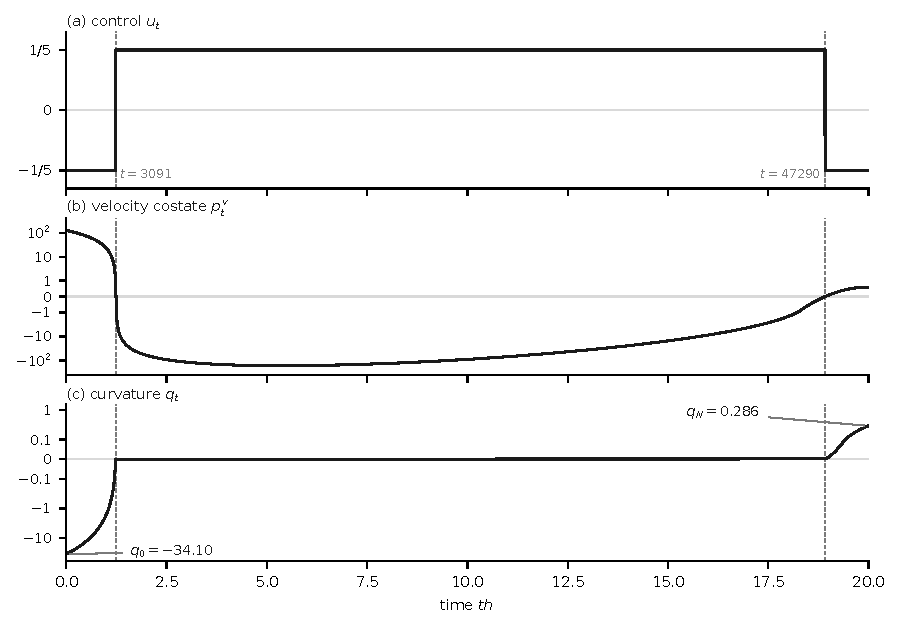
\includegraphics[width=0.85\textwidth]{fig-optcdeg2-calibration}
\caption{Split data of the \inst{optcdeg2} certificate against time $th$.
(a)~Control $u_t$ of the certified trajectory.
(b)~Velocity costate $p^v_t$; it is positive on both arcs with $u=-\frac15$.
(c)~Curvature $q_t$ of the split functions; it is zero on the middle arc and at both switching stages (dashed lines, $t=3091$ and $t=47290$).
Panels (b) and (c) use a symmetric logarithmic scale, linear near~0.
Data: the stored binary64 split data.}
\label{fig:optcdeg2-calibration}
\end{figure}

\begin{proof}[Proof of \cref{thm:optcdeg2-bound}]
Apply \cref{lem:optcdeg2-krotov} with the functions \eqref{eq:optcdeg2-S} and the intervals $V_t$ of \cref{lem:optcdeg2-enclosure}.
For $1\le t\le N-1$, \cref{lem:optcdeg2-stage} applies because $A>0$ at every stage, which the computation checks exactly.
It reduces $m_t$ to the minimization of two polynomials of degree at most $4$ over $V_t$; the third term never arises, because at every stage either $K_2\le0$ or a computed superset of the vertex set is empty.
Polynomials of degree at most $2$ are minimized in closed form.
For the 11,596 quartics, an exact Sturm sequence of $G'$ isolates its distinct real roots in $(\alpha,\beta)$, after an exact check that $G'(\alpha)G'(\beta)\ne0$.
For each root at which $G'$ changes sign from negative to positive, a bracket with $G'(l)<0<G'(r)$ is checked exactly, with floating-point roots used only as seeds (7,785 brackets; no bisection fallback and no root of even multiplicity was needed).
\Cref{lem:optcdeg2-quartic}, with $M_k$ the sum of the absolute coefficients of $G''$ times powers of $\max(|l_k|,|r_k|)$ (in the shifted variable $v-\bar v_t$), then gives a rational $\tilde m_t\le m_t$; the largest slack $M_k(r_k-l_k)^2$ is \sci{9.5}{-29}.
The end terms are explicit: $m_0$ is the minimum of a quadratic in $u$ over $U$ (about $1014.99647$), and $m_N=-(p^y_N)^2/(4w)-\tfrac12q_N\bar v_N^2=-(p^y_N)^2/(2h)$ because $\bar v_N=0$ (about $-1.86\cdot10^{-4}$).
Rounding $m_0$, every $\tilde m_t$ and $m_N$ down to the grid $2^{-200}$ and summing exactly gives a rational $B\le\vstar$ with $B\ge293.87607509587509237940$, the rigorous evaluation in \cref{thm:optcdeg2-bound}; its truncated display is $293.87607509587509237$.
All arithmetic is in Python integers and \texttt{Fraction}.
With the upper bound of \cref{prop:optcdeg2-point}, $\gapabs\le\sci{8.98}{-16}$ and $\gaprel\le\sci{3.06}{-18}$.
\end{proof}

The computation also checks the reduction of \cref{lem:optcdeg2-stage} against the definition of $\rho_t$, exactly, at three points $(v,u)$ in each of 115 stages, among them the seven stages around each switch.

Two further checks support the exact code and are not part of the proof.
A separately written sampling search over 197 stages found no point below the computed stage minimum (best values within \sci{2.8}{-29} of it).
Along the certified trajectory rounded to $2^{-300}$ at each step (near-feasible, not exactly feasible), every stage residual is at least its computed minimum, and the differences sum to $8.978\cdot10^{-16}$, the gap between $B$ and the upper bound of \cref{prop:optcdeg2-point}; stage 3091 accounts for about \sci{8.9777}{-16}, stage 47290 for about \sci{4.08}{-20} and every other stage for at most \sci{7.2}{-25}, the two stages with fractional control, where $p^v_{t+1}$ is small but not zero (\sci{7.6}{-12} and $-\sci{9.7}{-16}$).
The verification principle is classical (\cref{sec:split-framework}); the model-specific function and its exact check are the contribution.

\begin{certbox}[Certificate for \cref{thm:optcdeg2-bound}]
\certitem{Inputs}{OSIL file (SHA-256 \texttt{6a9bcd91}); split data (\texttt{08311d33}).}
\certitem{Computation}{$V_t$ on the grid $2^{-110}$; 11,596 quartic pieces by exact Sturm isolation; floors on the grid $2^{-200}$ summed exactly; \arith{E}.}
\certitem{Data reading}{exact decimals, asserted by the reader; a separately written reader and an exact comparison with the GAMS text confirm every row, bound and objective term.}
\certitem{Implementations}{the second code (exact) certifies the displayed bound; the first code, in binary64 intervals (\arith{F}, 162 geometric cells per stage, refined by bisection), certifies the weaker $293.8760750958728$, each stage bound at least \sci{3.6}{-19} below the exact one.}
\certitem{Evidence level}{\evid{stored}.}
\certitem{Replay}{Tier~1; 6\,s and 19\,s (enclosure and stage minima; 16 to 18\,s for the latter in other runs); 8\,s for the interval code.}
\end{certbox}

% ---------------------------------------------------------------------------
\subsubsection{\inst{optcdeg2}: the exactly feasible point}\label{app:optcdeg2-point}

\begin{proposition}[an exactly feasible point]\label{prop:optcdeg2-point}
Let $u_t=-\tfrac15$ for $t\le3090$ and $t\ge47291$, $u_t=\tfrac15$ for $3092\le t\le47289$, $u_{3091}=1506828432880435/2^{55}\approx0.041823$, and let $u_{47290}=\sigma$ be free.
Let $y_t(\sigma),v_t(\sigma)$ be defined by the rows of \eqref{eq:optcdeg2-model} from $y_0=10$, $v_0=0$.
For a rational $\tilde\sigma\approx0.0951284142971001$, there is $\sigma^*\in[\tilde\sigma-10^{-60},\tilde\sigma+10^{-60}]$ such that the resulting point is exactly feasible, and its objective is at most $293.87607509587509328$.
\end{proposition}

\begin{proof}
For every $\sigma$, all rows hold by construction, and $y_0=10$, $v_0=0$.
All controls lie in $U$ for $\sigma$ in the bracket.
The function $\sigma\mapsto v_N(\sigma)$ is a polynomial, hence continuous.
An interval simulation of the rows in integer arithmetic, with all quantities scaled by $2^{320}$ and rounded by floor and ceiling, gives $v_N<0$ at the left end of the bracket and $v_N>0$ at the right end (about $\mp3.8\cdot10^{-64}$).
Over the whole bracket it gives $v_t(\sigma)\ge-0.8316$ for $1\le t\le N-1$ and encloses the objective in an interval of width below \sci{4.8}{-64} whose upper end is $293.8760750958750932772142114247080159340995594910\ldots$.
By the intermediate value theorem, some $\sigma^*$ in the bracket gives $v_N=0$; the point is then exactly feasible, and its objective lies in the enclosure.
\end{proof}

The control of the certified point is $\pm\tfrac15$ except at stages 3091 and 47290; we claim this structure only for the certified point, not for every minimizer.
Our floating-point KKT point violates rows by up to \sci{8.9}{-16}, and its objective $293.87607509588105$ lies at least \sci{5.95}{-12} above the upper bound of \cref{prop:optcdeg2-point}; this says nothing about attainability.

\begin{certbox}[Certificate for \cref{prop:optcdeg2-point}]
\certitem{Inputs}{OSIL file (SHA-256 \texttt{6a9bcd91}); control vector (binary64, \texttt{8206c29d}).}
\certitem{Computation}{interval simulation of all rows over the bracket on the grid $2^{-320}$; sign change of $v_N$; bounds; objective enclosure; \arith{E}.}
\certitem{Data reading}{exact decimals, asserted as rationals.}
\certitem{Implementations}{the integer code certifies the displayed upper bound, which therefore does not depend on \texttt{mpmath}; a separately written \texttt{mpmath} code (\arith{I}, 200 bits, bracket of half-width $10^{-40}$) certifies the same display.}
\certitem{Evidence level}{\evid{stored}.}
\certitem{Replay}{Tier~1; 1.5\,s (integer code) and 9\,s (\texttt{mpmath} code).}
\end{certbox}

% ---------------------------------------------------------------------------
\subsubsection{\inst{optcdeg2}: MINOTAUR's report}\label{app:optcdeg2-minotaur}

\Cref{sec:solvers-invalid} proves \cref{prop:minotaur-optcdeg2} from \cref{prop:optcdeg2-point}, and \cref{app:solvers-published} compares the files and the log.
According to the log, the report occurs in the first presolve, before MINOTAUR's quadratic handler assigns default bounds to unbounded variables, so such default bounds play no role; the cause of the report is unknown, and we attribute no defect to MINOTAUR.

% Plan: development/outline.md, section 6, item B.3.
% Round-1 revision (adjudication G5): one certificate box per result, the
% verification record merged into the boxes.
\subsection{The \inst{camshape} instances}\label{app:camshape}

This subsection proves \cref{thm:camshape-opt}, \cref{lem:camshape-sturm,lem:camshape-envelope} and \cref{prop:camshape-deficit}, and it determines the exact optima of the four rounded QPLIB copies used in \cref{prop:qplib-copies}.

\subsubsection{Model and data}\label{app:camshape-model}

The instances come from problem~4 of COPS~2.0 \citep{dolan2001-benchmarking-optimization-software-with-cops}.
MINLPLib's \inst{camshape100}, \inst{camshape200}, \inst{camshape400} and \inst{camshape800} are scalar forms of the GAMS model library model \texttt{camshape} \citep{library2026-cops-and-gams-source-models}, negated to a minimization.
Their model is~\eqref{eq:camshape-problem} of \cref{sec:other-camshape}, with the radii $r_j = \texttt{x}\langle j\rangle$ at the angles $j\Delta\theta$ and the slope variables $d_i = \texttt{x}\langle n+i\rangle$, all continuous; the COPS radii $r_0 = 1$ and $r_{n+1} = 2$ are constants, so $G_1$ reads $-r_1 + c\,r_2 - r_1 r_2 \le 0$, and $d_1$ is free.
The rows are $G_j = \texttt{e}\langle j\rangle$ ($2 \le j \le n-1$), $G_1 = \texttt{e}\langle n\rangle$, $G_n = \texttt{e}\langle n+1\rangle$, $H = \texttt{e}\langle n+2\rangle$ and $D_i = \texttt{e}\langle n+2+i\rangle$.
$G_1,\dots,G_n$ and $H$ are the COPS convexity condition $2\cos(\Delta\theta)\,r_{j-1}r_{j+1} \le r_j(r_{j-1}+r_{j+1})$ for $j = 1,\dots,n+1$ (with $r_{n+2} = r_n$), which says that the point $(r_j, j\Delta\theta)$ lies on or outside the chord through its neighbours.
The bound $\bar u$ is the same condition at $j = 0$ (with $r_{-1} = r_0 = 1$), and $\ell$ and $\alpha$ come from the curvature condition.
The GAMS source does not bound $d_1$, so MINLPLib omits the COPS curvature condition $|r_2 - r_1| \le \alpha$; it is slack at the optimum (\cref{app:camshape-proof}).
\Cref{tab:camshape-constants} lists the stored decimals, which approximate the values given in \cref{sec:other-camshape}; the proofs use only the stored decimals.
In every file $c_H = c$, and $c_2 = 2c$ except for $n = 400$ ($c_2 - 2c = -10^{-14}$).

\begin{table}[ht]
\centering
\small
\caption{Constants of the stored \inst{camshape} models (OSIL decimals; the \texttt{.gms} files are identical).}
\label{tab:camshape-constants}
\begin{tabular}{@{}lllll@{}}
\toprule
 & $n = 100$ & $n = 200$ & $n = 400$ & $n = 800$ \\
\midrule
$c_0$ & 0.0314159265358979 & 0.015707963267949 & 0.00785398163397448 & 0.00392699081698724 \\
$c = c_H$ & 1.99984519984971 & 1.99996091355262 & 1.99999017956722 & 1.99999753875636 \\
$c_2$ & 3.99969039969942 & 3.99992182710524 & 3.99998035913443 & 3.99999507751272 \\
$\bar u$ & 1.00015482411709 & 1.00003908797519 & 1.00000982052922 & 1.0000024612497 \\
$\ell$ & 1.98133707334501 & 1.99062211148182 & 1.99529936261308 & 1.99764674707596 \\
$\alpha$ & 0.0186629266549889 & 0.00937788851817849 & 0.0047006373869174 & 0.0023532529240373 \\
\bottomrule
\end{tabular}
\end{table}

All radii are positive on the feasible set, because the lower bounds are $1$ and $\ell > 0$.
Dividing $G_1$ by $r_1r_2$ and $G_j$ by $r_{j-1}r_jr_{j+1}$ therefore turns $G_1,\dots,G_{n-1}$ into the rows $e_j(u) \ge 0$ ($1 \le j \le n-1$) of \cref{sec:other-camshape}, which are linear in $u_j = 1/r_j$, with $u_0 = 1$.
Since the objective decreases in every radius, the problem asks for the largest feasible radii.

\subsubsection{Recurrences, finite checks and the optimal value}\label{app:camshape-proof}

We state the objects and checks of \cref{sec:other-camshape} for arbitrary rational constants $c_0, c, c_2, c_H, \bar u, \ell, \alpha$ in a model of the form~\eqref{eq:camshape-problem}; the MINLPLib files and the QPLIB copies are instances.

\begin{definition}[comparison sequence and envelope]\label{def:camshape-envelope}
In exact rational arithmetic, let $U_0 = 1$, $U_1 = c$, $U_{m+1} = c\,U_m - U_{m-1}$ (so $U_m$ is the Chebyshev polynomial of the second kind at $c/2$), and $S_0 = 1$, $S_1 = 1/\bar u$, $S_{j+1} = c\,S_j - S_{j-1}$ for $1 \le j \le n-1$.
Let $R_j = 1/S_j$ if $S_j > 0$ and $R_j = +\infty$ otherwise, $b_1 = \bar u$, $b_j = 2$ for $j \ge 2$, and $B_j = \min(R_j, b_j)$.
The envelope is $E_1 = B_1$ and $E_j = \min_{2 \le k \le n}(B_k + \alpha|j-k|)$ for $2 \le j \le n$; put $d^E_i = E_{i+1} - E_i$ and $v_n = -c_0\sum_{j=1}^n E_j$.
The finite checks are:
(K1) $U_m \ge 0$ for $0 \le m \le n-1$;
(K2) $0 < S_j \le 1$ for $1 \le j \le n$;
(K3) $E_{n-1} = E_n = 2$;
(K4) $\bar u \le 1 + \alpha$;
(K5) $c_0 > 0$, $1 \le \bar u \le 2$, $0 < c < 2$, $c_2 \le 4$ and $0 < \ell \le 2$;
(K6) $c_H \le 2$.
\end{definition}

Since $R_1 = \bar u = b_1$, $E_1 = \bar u$; (K4) and (K5) give $\alpha \ge \bar u - 1 \ge 0$.
For $\alpha \ge 0$ the envelope is a forward pass $F_2 = B_2$, $F_j = \min(B_j, F_{j-1} + \alpha)$ followed by a backward pass $E_n = F_n$, $E_j = \min(F_j, E_{j+1} + \alpha)$, so all quantities cost $O(n)$ rational operations.

\begin{lemma}[Green's function of the second difference]\label{lem:camshape-green}
Let $c \in \R$, let $U_m$ be defined from $c$ as in \cref{def:camshape-envelope}, let $N \ge 1$, and let $u_0,\dots,u_N$ and $s_0,\dots,s_N$ be real with $u_0 = s_0$ and $s_{j+1} = c\,s_j - s_{j-1}$ for $1 \le j \le N-1$.
Put $e_j = u_{j-1} - c\,u_j + u_{j+1}$ for $1 \le j \le N-1$.
Then for $1 \le j \le N$
\begin{equation}\label{eq:camshape-green}
u_j - s_j = U_{j-1}\,(u_1 - s_1) + \sum_{k=1}^{j-1} U_{j-1-k}\, e_k .
\end{equation}
If moreover $U_m \ge 0$ for $0 \le m \le N-1$, $u_1 \ge s_1$ and $e_k \ge -\beta$ for all $k$, with $\beta \ge 0$, then $u_j \ge s_j - \beta W_j$ for $0 \le j \le N$, where $W_0 = W_1 = 0$ and $W_j = \sum_{m=0}^{j-2} U_m$.
\end{lemma}

\begin{proof}
Put $z_j = u_j - s_j$.
Then $z_0 = 0$ and $z_{j+1} = c\,z_j - z_{j-1} + e_j$ for $1 \le j \le N-1$.
Formula~\eqref{eq:camshape-green} holds for $j = 1$ and $j = 2$ ($z_2 = c\,z_1 + e_1 = U_1 z_1 + U_0 e_1$).
If it holds for $j-1$ and $j$, where $2 \le j \le N-1$, then
\[
z_{j+1} = (c\,U_{j-1} - U_{j-2})\,z_1 + \sum_{k=1}^{j-2}(c\,U_{j-1-k} - U_{j-2-k})\,e_k + c\,U_0\,e_{j-1} + e_j = U_j z_1 + \sum_{k=1}^{j} U_{j-k}\,e_k ,
\]
which is~\eqref{eq:camshape-green} for $j+1$; the indices of $U$ that occur are at most $N-1$.
Under the additional hypotheses every term is at least $-\beta U_{j-1-k}$ or nonnegative, and $\sum_{k=1}^{j-1}U_{j-1-k} = W_j$.
\end{proof}

\begin{proof}[Proof of \cref{lem:camshape-sturm}]
Apply \cref{lem:camshape-green} with the given $N \le n$, $s = S$ and $\beta = 0$; $S$ satisfies the recurrence for $1 \le j \le N-1$.
The formula uses only $u_0 = 1 = S_0$; the inequality uses in addition (K1), $u_1 \ge S_1$ and $e_k(u) \ge 0$.
\end{proof}

The numbers $U_{j-1-k}$ are the Green's function of the second-difference operator with initial data at $0$ and $1$.
For $0 < c < 2$, $U_m = \sin((m+1)\varphi)/\sin\varphi$ with $\varphi = \arccos(c/2)$, so (K1) holds exactly when $n\varphi \le \pi$: the discrete form of disconjugacy \citep[see][for the discrete Sturm--Liouville theory]{bohner1996-linear-hamiltonian-difference-systems-disconjugacy}.
For the stored constants $n\varphi$ is close to $0.4\pi$; the computation checks (K1) directly.

\begin{lemma}[min-plus envelope]\label{lem:camshape-minplus}
If $r \in \R^n$ satisfies $r_j \le B_j$ for all $j$ and $|r_{j+1} - r_j| \le \alpha$ for $2 \le j \le n-1$, then $r \le E$.
\end{lemma}

\begin{proof}
$r_1 \le B_1 = E_1$.
For $j, k \ge 2$ every consecutive pair between $j$ and $k$ is slope-constrained, so $r_j \le r_k + \alpha|j-k| \le B_k + \alpha|j-k|$; minimize over $k$.
\end{proof}

\begin{lemma}[the envelope point is feasible]\label{lem:camshape-feasible}
If (K2)--(K6) hold, then $(E, d^E)$ is feasible for~\eqref{eq:camshape-problem}.
\end{lemma}

\begin{proof}
\emph{Bounds and linear rows.}
By (K2) and (K5), $R_k \ge 1$ and $b_k \ge 1$, so $B_k \ge 1$ and $E_j \ge 1$ (as $\alpha \ge 0$); also $E_j \le B_j \le b_j$, $E_1 = \bar u$, and $E_n = 2 \ge \ell$ by (K3) and (K5).
The rows $D_i$ hold by definition of $d^E$.
On $\{2,\dots,n\}$, $E$ is a minimum of $\alpha$-Lipschitz functions, so $|d^E_i| \le \alpha$ for $i \ge 2$.

\emph{Rows $H$ and $G_n$.}
With $E_n = 2$, $H$ reads $4c_H - 8 \le 0$, which holds since $c_H \le 2$, and $G_n$ reads $(c_2 - 2)E_{n-1} - 4 \le 2\max(c_2 - 2, 0) - 4 \le 0$ since $1 \le E_{n-1} \le 2$ and $c_2 \le 4$.

\emph{Rows $G_1,\dots,G_{n-1}$.}
They are equivalent to $e_j(w) \ge 0$ for $w_j = 1/E_j$, $w_0 = 1$, and $E \le R$ gives $w \ge S$.
Fix $1 \le j \le n-1$.
If $E_j = R_j$, then $w_j = S_j$ and $e_j(w) \ge S_{j-1} - cS_j + S_{j+1} = 0$.
Otherwise $j \ge 2$, and we show $E_{j-1} + E_{j+1} \le 2E_j$.
If $E_j = B_j$, then $E_j = b_j = 2 \ge E_k$ for all $k$ (recall $E_1 = \bar u \le 2$).
If $E_j < B_j$, then $E_j = B_k + \alpha|j-k|$ for some $k \ge 2$, $k \ne j$.
For $k < j$, $E_{j-1} \le B_k + \alpha(j-1-k) = E_j - \alpha$ and $E_{j+1} \le E_j + \alpha$ (Lipschitz).
For $k > j$, $E_{j+1} \le E_j - \alpha$ likewise, and $E_{j-1} \le E_j + \alpha$: by the Lipschitz property if $j \ge 3$, and for $j = 2$ because $E_1 = \bar u \le 1 + \alpha \le E_2 + \alpha$ by (K4).
By the inequality between arithmetic and harmonic means, $w_{j-1} + w_{j+1} \ge 4/(E_{j-1} + E_{j+1}) \ge 2/E_j = 2w_j$, so $e_j(w) \ge (2 - c)\,w_j > 0$.
\end{proof}

\Cref{lem:camshape-envelope} consists of \cref{lem:camshape-minplus,lem:camshape-feasible}.

\begin{proposition}[optimal value for general constants]\label{prop:camshape-general}
Consider a model of the form~\eqref{eq:camshape-problem} with rational constants.
\begin{enumerate}
\item[(a)] If (K1) holds and $c_0, \bar u, \ell > 0$, then every feasible $(r,d)$ satisfies $r \le E$, and hence $f(r,d) \ge v_n$, where $f$ is the objective.
\item[(b)] If (K2)--(K6) hold, then $(E, d^E)$ is feasible and $f(E, d^E) = v_n$.
\item[(c)] Under both sets of hypotheses, $v_n$ is the optimal value, $(E, d^E)$ is the only optimal solution, and $E$ is the componentwise greatest feasible radius vector; so $(E, d^E)$ also maximizes every componentwise nondecreasing function of $r$ over the feasible set.
\end{enumerate}
\end{proposition}

\begin{proof}
(a) The bounds give $r_j \ge 1$ for $j < n$ and $r_n \ge \ell > 0$.
With $u = 1/r$ and $u_0 = 1$, the rows $G_1,\dots,G_{n-1}$ give $e_j(u) \ge 0$, and $r_1 \le \bar u$ gives $u_1 \ge S_1$.
\Cref{lem:camshape-green} and (K1) give $u \ge S$, so $r_j \le R_j$ when $S_j > 0$, and with $r_j \le b_j$ we get $r \le B$.
The rows $D_j$ and $|d_j| \le \alpha$ give $|r_{j+1} - r_j| \le \alpha$ for $j \ge 2$, and \cref{lem:camshape-minplus} gives $r \le E$.
Since $c_0 > 0$, $f(r,d) \ge -c_0\sum_j E_j = v_n$.
(b) is \cref{lem:camshape-feasible}.
(c) By (a) and (b) the bound $v_n$ is attained.
If $f(r,d) = v_n$, then $\sum_j r_j = \sum_j E_j$ and $r \le E$, so $r = E$, and the rows $D_i$ give $d = d^E$.
\end{proof}

Part (a) uses only the rows $G_1,\dots,G_{n-1}$, the upper bounds, positivity and the slope rows for $j \ge 2$; the rows $G_n$, $H$, $D_1$ and the values of $c_2$ and $\ell$ (beyond $\ell > 0$) do not enter.

\begin{proof}[Proof of \cref{thm:camshape-opt}]
For each $n$ we read the constants of \cref{tab:camshape-constants} from the OSIL file as exact rationals, assert that the file has the form~\eqref{eq:camshape-problem}, and evaluate (K1)--(K6) and $v_n$ in exact rational arithmetic.
All checks pass, and \cref{prop:camshape-general}(c) gives the claims.
\Cref{tab:camshape-values} shows the floor and ceiling of the rational $v_n$ (for $n = 100$ its denominator has 28,165 digits); no rounding enters before the final display.
\end{proof}

\begin{table}[ht]
\centering
\small
\caption{Exact optima of the \inst{camshape} instances (attained, so $\gapabs = 0$) and the structure of $E$. Floor and ceiling of $v_n$ at 14 decimals; phases $E_j = R_j$ (contact), $E_j = E_{j-1} + \alpha$ (maximal slope) and $E_j = 2$; number of rows $G_j$ active at $E$.}
\label{tab:camshape-values}
\begin{tabular}{@{}rllrrrr@{}}
\toprule
$n$ & floor of $v_n$ & ceiling of $v_n$ & contact & max.\ slope & $E_j = 2$ & active rows \\
\midrule
100 & $-4.28414712174675$ & $-4.28414712174674$ & 1--64 & 65--94 & 95--100 & 63 \\
200 & $-4.27850023299273$ & $-4.27850023299272$ & 1--128 & 129--187 & 188--200 & 127 \\
400 & $-4.27568847892555$ & $-4.27568847892554$ & 1--256 & 257--374 & 375--400 & 255 \\
800 & $-4.27427414195420$ & $-4.27427414195419$ & 1--513 & 514--749 & 750--800 & 512 \\
\bottomrule
\end{tabular}
\end{table}

For $0 < c < 2$, $S_j = A\cos(j\varphi) + A'\sin(j\varphi)$, so the points with polar coordinates $(R_j, j\varphi)$ lie on one straight line; for the unrounded COPS constants it extends the last chord of the base circle.
In the cam picture, \cref{lem:camshape-sturm} says that a discretely convex arc starting on the base circle cannot pass outside this line.
The exact computation shows the three phases of \cref{tab:camshape-values}: $E$ follows the line up to the last index $m$ with $R_m - R_{m-1} \le \alpha$, then $E_j = \min(R_m + \alpha(j-m), 2)$.
The omitted COPS condition is slack: $|E_2 - E_1| \le 3.10\cdot10^{-4}$, $7.82\cdot10^{-5}$, $1.97\cdot10^{-5}$ and $4.93\cdot10^{-6}$ for the four sizes, far below $\alpha$.

\begin{certbox}[Certificate for \cref{thm:camshape-opt}]
\certitem{Inputs}{OSIL files (SHA-256 \texttt{9e17da72}, \texttt{76d6141d}, \texttt{a53174a4}, \texttt{d0692d0f}).}
\certitem{Computation}{(K1)--(K6), the rational $v_n$ and every row and bound at $(E,d^E)$; \arith{E}; no floating point or branching.}
\certitem{Data reading}{exact, by three separately written readers (two match a template, one evaluates every row generically and checks the case split of \cref{lem:camshape-feasible} row by row).}
\certitem{Implementations}{three separately written codes, two exact (printing $v_n$ to 20 and 30 digits) and one in fixed point with directed rounding at scale $10^{-120}$, agree on $v_n$ to all printed digits; all find zero violation at $(E,d^E)$, the third for $n=100$ and $200$ only.}
\certitem{Evidence level}{\evid{hand}+\evid{stored}.}
\certitem{Replay}{Tier~1; 8\,s for all four sizes (6\,min and under 2\,s for the other codes).}
\end{certbox}

\begin{remark}[sensitivity to the constants]\label{rem:camshape-robust}
The certificate is monotone in the constants: for $u > 0$ the rows $e_j(u) \ge 0$ become stronger as $c$ grows, the bounds on $r_1$ and on the slopes become stronger as $\bar u$ and $\alpha$ shrink, and $f$ decreases as $c_0$ grows.
Write $E(c, \bar u, \alpha)$ for the envelope built from these three constants.
Every feasible point of a model of the form~\eqref{eq:camshape-problem} with $\ell > 0$, $c \ge c^-$, $\bar u \le \bar u^+$, $\alpha \le \alpha^+$ and $0 < c_0 \le c_0^+$ satisfies the relaxed rows with the corner constants $(c^-, \bar u^+, \alpha^+)$; if (K1) holds at $c^-$, the proof of \cref{prop:camshape-general}(a) bounds the optimal value from below by $-c_0^+\sum_j E_j(c^-, \bar u^+, \alpha^+)$.
Conversely, suppose that the corner envelope $E^+ = E(c^+, \bar u^-, \alpha^-)$ satisfies every row and bound of the model with the corner constants and has $E^+_{n-1} = E^+_n = 2$.
A model with $c \le c^+$, $\bar u \ge \bar u^-$, $\alpha \ge \alpha^-$, $c_0 \ge c_0^- > 0$, $c_2 \le 4$, $c_H \le 2$ and $\ell \le 2$ has weaker rows $G_1, \dots, G_{n-1}$, bound on $r_1$ and slope bounds than the corner model, and its rows $G_n$ and $H$ and its bounds on $r_n$ hold at $E^+$ as in the proof of \cref{lem:camshape-feasible}; so $(E^+, d^{E^+})$ is feasible for it, and its optimal value is at most $-c_0^-\sum_j E^+_j$.
For $c^\pm$, $\bar u^\pm$, $\alpha^\pm$ and $c_0^\pm$ at distance $10^{-14}$ from the stored constants, we checked (K1) at $c^-$ and the hypotheses on $E^+$ in exact arithmetic, by evaluating every row and bound at $E^+$.
With the corner sums, this shows that every model of the form~\eqref{eq:camshape-problem} whose seven constants each differ from the stored ones by at most $10^{-14}$ has an optimal value within $5.9\cdot10^{-11}$, $2.3\cdot10^{-10}$, $9.0\cdot10^{-10}$ and $3.6\cdot10^{-9}$ of $v_n$ for $n = 100, 200, 400, 800$; a second implementation reproduced the endpoints for $n = 100$ and $800$ and for two copies of \cref{app:camshape-copies}.
This concerns perturbed models of the same structure; it does not extend the exact values of \cref{thm:camshape-opt} to other readings of the data.
\end{remark}

\subsubsection{Tolerance-feasible points: the deficit bound}\label{app:camshape-deficit}

Let $0 \le \varepsilon < 1$, and call a point $\varepsilon$-feasible if every row and bound of~\eqref{eq:camshape-problem} is violated by at most $\varepsilon$ (\cref{def:sem-feasible}); the objective is evaluated exactly.
Put $\beta_\varepsilon = \varepsilon/(1-\varepsilon)^3$ and define $S^\varepsilon$ by $S^\varepsilon_0 = 1$, $S^\varepsilon_1 = 1/(\bar u + \varepsilon)$ and the recurrence of $S$; $R^\varepsilon_j = 1/(S^\varepsilon_j - \beta_\varepsilon W_j)$ if this denominator is positive and $+\infty$ otherwise; caps $b^\varepsilon_1 = \bar u + \varepsilon$ and $b^\varepsilon_j = 2 + \varepsilon$; $B^\varepsilon = \min(R^\varepsilon, b^\varepsilon)$; and the envelope $E^\varepsilon$ of \cref{def:camshape-envelope} with $B^\varepsilon$ and slope $\alpha + 2\varepsilon$.
Set $D_n(\varepsilon) = c_0\sum_j(E^\varepsilon_j - E_j)$, an explicit bound, rational when $\varepsilon$ is rational, with $D_n(0) = 0$ and $v_n - D_n(\varepsilon) = -c_0\sum_j E^\varepsilon_j$.

\begin{proof}[Proof of \cref{prop:camshape-deficit}]
Let $(r,d)$ be $\varepsilon$-feasible.
All lower bounds in~\eqref{eq:camshape-problem} are at least $1$ (in all four files $\ell \ge 1$), so $r_j \ge 1 - \varepsilon > 0$.
Dividing $G_j$ ($2 \le j \le n-1$) by $r_{j-1}r_jr_{j+1} \ge (1-\varepsilon)^3$ and $G_1$ by $r_1r_2 \ge (1-\varepsilon)^2$ gives $e_j(u) \ge -\beta_\varepsilon$ for $u = 1/r$, and $r_1 \le \bar u + \varepsilon$ gives $u_1 \ge S^\varepsilon_1$.
\Cref{lem:camshape-green} with $s = S^\varepsilon$, $\beta = \beta_\varepsilon$ and (K1), which holds for the four files by \cref{thm:camshape-opt}, gives $u_j \ge S^\varepsilon_j - \beta_\varepsilon W_j$, so $r \le B^\varepsilon$.
For $i \ge 2$, $|d_i| \le \alpha + \varepsilon$ and $|r_i - r_{i+1} + d_i| \le \varepsilon$ give $|r_{i+1} - r_i| \le \alpha + 2\varepsilon$.
\Cref{lem:camshape-minplus} with slope $\alpha + 2\varepsilon$ gives $r \le E^\varepsilon$, hence $f(r,d) \ge v_n - D_n(\varepsilon)$.
\end{proof}

The computation evaluates the construction exactly and rounds each $R^\varepsilon_j$ up to a fine dyadic grid, which keeps an upper bound on $D_n(\varepsilon)$.
Two separately written implementations agree on every value in \cref{tab:camshape-deficit}, and a third reproduces those it recomputed.
For the tabulated $\varepsilon \le 10^{-8}$ the ratio $D_n(\varepsilon)/(n^2\varepsilon)$ is at most $0.605$, and it is smaller for larger $\varepsilon$ (on \inst{QPLIB_3177}, $D(10^{-6}) \approx 0.43\,n^2\varepsilon$).
$D_n(\varepsilon)$ is a proved upper bound, not the worst case: the explicit $\varepsilon$-feasible points of the last column, which violate every $G_j$ by $\varepsilon$ and use the caps $2 + \varepsilon$ and the slopes $\alpha + 2\varepsilon$, reach about 87\% of it (numerical evidence).
MINLPLib's points p2 for \inst{camshape400} and \inst{camshape800} violate row $G_1$ by $3.0\cdot10^{-10}$, and 360 and 722 rows by more than $10^{-12}$, most by about $10^{-10}$; \cref{sec:other-camshape} gives their deficits, and \cref{app:solvers-points} compares the points returned in our runs with $D_n$.

\begin{table}[ht]
\centering
\small
\caption{Upper bounds on the deficit of $\varepsilon$-feasible points (\cref{prop:camshape-deficit}) and their ratio to $n^2\varepsilon$, rounded up; fraction of $D_n(\varepsilon)$ reached by explicit $\varepsilon$-feasible points built in floating point (numerical evidence, rounded down).}
\label{tab:camshape-deficit}
\begin{tabular}{@{}rrlrr@{}}
\toprule
$n$ & $\varepsilon$ & $D_n(\varepsilon) \le$ & $D_n(\varepsilon)/(n^2\varepsilon)$ & reached \\
\midrule
100 & $10^{-10}$ & $6.05\cdot10^{-7}$ & 0.605 & 87.3\% \\
100 & $10^{-8}$ & $6.05\cdot10^{-5}$ & 0.605 & 87.3\% \\
200 & $10^{-10}$ & $2.36\cdot10^{-6}$ & 0.589 & 87.3\% \\
400 & $10^{-10}$ & $9.35\cdot10^{-6}$ & 0.585 & 87.3\% \\
400 & $3\cdot10^{-10}$ & $2.81\cdot10^{-5}$ & 0.585 & 87.3\% \\
800 & $3\cdot10^{-10}$ & $1.13\cdot10^{-4}$ & 0.587 & 87.2\% \\
\bottomrule
\end{tabular}
\end{table}

\subsubsection{The rounded QPLIB copies}\label{app:camshape-copies}

QPLIB contains the four models as \inst{QPLIB_2738}, \inst{QPLIB_2480}, \inst{QPLIB_2703} and \inst{QPLIB_3177} \citep{furini2018-qplib-a-library-of-quadratic,cache2026-qplib-pages-and-rounded-camshape}, with another variable order and constants rounded to 8--10 digits (for example $c = 1.9998452$ for $n = 100$).
They are different models, so \cref{thm:camshape-opt} does not apply to them, but \cref{prop:camshape-general} does.

\begin{proposition}[exact optima of the QPLIB copies]\label{prop:camshape-copies}
Read with exact decimals, the \texttt{.gms} files of the four copies have the form~\eqref{eq:camshape-problem}, and (K1)--(K6) hold.
Hence each copy's optimal value is the rational $-c_0\sum_j E_j$ of its own constants, attained at its own envelope point, with the values and shifts of \cref{tab:camshape-copies}.
QPLIB's reference points \citep{furini2026-qplib-official-solution-point-records} for \inst{QPLIB_2703} and \inst{QPLIB_3177} violate row $G_1$ by $3.0\cdot10^{-10}$ and lie at least $8.15\cdot10^{-6}$ and $3.27\cdot10^{-5}$ below their copies' optima; the one for \inst{QPLIB_2738} violates rows by up to $2.0\cdot10^{-14}$ and lies more than $5.8\cdot10^{-14}$ below; the one for \inst{QPLIB_2480} violates rows by up to $2.2\cdot10^{-14}$ and lies about $1.5\cdot10^{-12}$ above.
\end{proposition}

\begin{proof}
The structure and the checks are verified in exact rational arithmetic, and \cref{prop:camshape-general}(c) gives the optima; the remaining claims follow by exact evaluation of each point in its own copy and exact subtraction.
\end{proof}

\begin{table}[ht]
\centering
\small
\caption{Exact optima of the rounded QPLIB copies (floor and ceiling at 16 decimals), shift above the MINLPLib optimum $v_n$ (rounded down), and position of QPLIB's reference point.}
\label{tab:camshape-copies}
\begin{tabular}{@{}lllll@{}}
\toprule
copy & floor of optimum & ceiling of optimum & shift $\ge$ & reference point \\
\midrule
\inst{QPLIB_2738} & $-4.2841462678046117$ & $-4.2841462678046116$ & $8.539\cdot10^{-7}$ & ${>}\,5.8\cdot10^{-14}$ below \\
\inst{QPLIB_2480} & $-4.2784904096736786$ & $-4.2784904096736785$ & $9.823\cdot10^{-6}$ & about $1.5\cdot10^{-12}$ above \\
\inst{QPLIB_2703} & $-4.2756507125126530$ & $-4.2756507125126529$ & $3.776\cdot10^{-5}$ & $\ge 8.15\cdot10^{-6}$ below \\
\inst{QPLIB_3177} & $-4.2741871514717434$ & $-4.2741871514717433$ & $8.699\cdot10^{-5}$ & $\ge 3.27\cdot10^{-5}$ below \\
\bottomrule
\end{tabular}
\end{table}

\begin{certbox}[Certificate for \cref{prop:camshape-copies}]
\certitem{Inputs}{QPLIB \texttt{.gms} copies (SHA-256 \texttt{b30f2827} for 2738, \texttt{2ca3dde5} for 2480, \texttt{0ac46c15} for 2703, \texttt{4d0e595f} for 3177); reference points \texttt{1d903458}, \texttt{18a8e5bf}, \texttt{7052af94}, \texttt{115ae675}.}
\certitem{Computation}{structure assertions; (K1)--(K6), envelope and optimum; every row and bound at the envelope and reference points; \arith{E}.}
\certitem{Data reading}{exact decimals.}
\certitem{Implementations}{two separately written GAMS parsers, the first checking every row at the envelope point and the second applying \cref{prop:camshape-general}, print identical 16-decimal floors; an earlier code for the lower bounds agrees.}
\certitem{Evidence level}{\evid{hand}+\evid{stored}.}
\certitem{Replay}{Tier~1; under 2\,s for the second parser, which also evaluates the reference points; about 10\,min for the first on the four copies and the four MINLPLib files together, and about 5\,min for its evaluation of the reference points.}
\end{certbox}

All four copies round $c$ up, which tightens every convexity row, and the net effect of all roundings raises the optimum in each case, by about $2\cdot10^{-7}$ to $2\cdot10^{-5}$ relative; the MINLPLib optima are not feasible for the copies.
The deficit construction of \cref{app:camshape-deficit}, applied to the copies with the same exact arithmetic and upward rounding, shows that every point of \inst{QPLIB_2738} with violations at most $2.5\cdot10^{-8}$ has objective at least $-4.2842974$, and every point of \inst{QPLIB_3177} with violations at most $8\cdot10^{-9}$ has objective at least $-4.2771732$ (both rounded down).
Both values lie above $-4.284301$ and $-4.2773$, which exceed every number within one unit of the last displayed digit of ANTIGONE's $-4.284302$ and MINOTAUR's $-4.2774$, so reaching these reported values needs larger violations (\cref{prop:qplib-copies}).

The listed and QPLIB points were evaluated exactly by two or three implementations each.
The ingredients are classical (polar convexity, discrete Sturm comparison, the greatest Lipschitz minorant on a path); what is new is their exact application to these stored models.

% Plan: development/outline.md, section 6, item B.4.
% Round-1 revision (adjudication G5): one certificate box per result, the
% verification record merged into the boxes.
\subsection{The \inst{chain} and \inst{catmix} instances}\label{app:chain}

This subsection proves \cref{thm:chain-bound,thm:catmix-bound}, whose certificates \cref{sec:split-richer} outlines; both families are trapezoidal discretizations of optimal control problems from COPS~2.0 \citep{dolan2001-benchmarking-optimization-software-with-cops}.

\subsubsection{The \inst{chain} model}\label{app:chain-model}

COPS~2.0 (problem~3) seeks the shape $x(t)$ of a chain of length $4$ between $(0,1)$ and $(1,3)$ that minimizes $\int_0^1 x\sqrt{1+x'^2}\,dt$ subject to $\int_0^1 \sqrt{1+x'^2}\,dt = 4$, written as a control problem with $u = x'$ and discretized by the trapezoidal rule on $N$ intervals.
MINLPLib's \inst{chain}$N$, $N\in\{50,100,200,400\}$, are the scalar forms of the GAMS model library model \texttt{chain} \citep{library2026-cops-and-gams-source-models}.
With $h = 1/N$ and $\eta = h/2$ the model is
\begin{equation}\label{eq:chain-model}
\begin{aligned}
\min\quad & f(x,u) = \eta \textstyle\sum_{i=0}^{N-1} \bigl( x_i\sqrt{1+u_i^2} + x_{i+1}\sqrt{1+u_{i+1}^2} \bigr)\\
\text{s.t.}\quad & x_{i+1} - x_i - \eta\,(u_i + u_{i+1}) = 0 \qquad (0 \le i \le N-1),\\
& \eta \textstyle\sum_{i=0}^{N-1} \bigl( \sqrt{1+u_i^2} + \sqrt{1+u_{i+1}^2} \bigr) = 4,\\
& x_0 = 1,\quad x_N = 3,\quad \text{all other variables free.}
\end{aligned}
\end{equation}
The OSIL files have $2N+2$ variables and $N+1$ rows; the decimal $\eta$ is exactly $1/(2N)$, and the objective constant is $0$.
No variable has finite bounds apart from the two fixed end values, so spatial branch and bound starts from an unbounded box.

\subsubsection{\texorpdfstring{\inst{chain}}{chain}: reduction to two end values}\label{app:chain-reduction}

\begin{lemma}[polyline form]\label{lem:chain-polyline}
Let $(x,u)$ satisfy the $N$ linear rows of~\eqref{eq:chain-model}.
Put $z_i = x_i - \eta u_i$ for $0 \le i \le N$ and $z_{N+1} = x_N + \eta u_N$.
Then $x_i = (z_i + z_{i+1})/2$ and $u_i = (z_{i+1} - z_i)/h$ for $0 \le i \le N$, and $(x,u) \mapsto z$ is a bijection from the solution set of the linear rows onto $\R^{N+2}$.
If moreover $x_0 = 1$ and $x_N = 3$, then $z_0 = 2 - z_1$ and $z_{N+1} = 6 - z_N$.
With
\[
\lambda_0 = \sqrt{\eta^2 + (z_1 - 1)^2},\qquad \lambda_N = \sqrt{\eta^2 + (3 - z_N)^2}
\]
and $\lambda_k = \sqrt{h^2 + (z_{k+1} - z_k)^2}$ for $1 \le k \le N-1$, the length row is equivalent to $\lambda_0 + \lambda_N + \sum_{k=1}^{N-1}\lambda_k = 4$, and
\begin{equation}\label{eq:chain-pieces}
f(x,u) = \lambda_0 + 3\lambda_N + \sum_{k=1}^{N-1} \lambda_k\, \frac{z_k + z_{k+1}}{2}.
\end{equation}
\end{lemma}

\begin{proof}
Row $i$ reads $x_{i+1} - \eta u_{i+1} = x_i + \eta u_i$, that is, $z_{i+1} = x_i + \eta u_i$ for $0 \le i \le N-1$; for $i = N$ this is the definition of $z_{N+1}$.
Adding and subtracting $z_i = x_i - \eta u_i$ and $z_{i+1} = x_i + \eta u_i$ gives $x_i$ and $u_i$.
Conversely, for any $z \in \R^{N+2}$ these formulas give $x_{i+1} - x_i = (z_{i+2} - z_i)/2 = \eta(u_i + u_{i+1})$, so the map is onto, and it is injective by construction.
The fixed values give $z_0 + z_1 = 2$ and $z_N + z_{N+1} = 6$.
Put $m_i = \sqrt{h^2 + (z_{i+1} - z_i)^2}$; then $\eta\sqrt{1+u_i^2} = m_i/2$.
The trapezoidal sums weight index $i$ by $\omega_0 = \omega_N = 1$ and $\omega_i = 2$ otherwise, so the length row reads $m_0/2 + \sum_{i=1}^{N-1}m_i + m_N/2 = 4$, and $f = x_0m_0/2 + \sum_{i=1}^{N-1} x_im_i + x_Nm_N/2$.
Finally $m_0 = 2\lambda_0$ because $z_1 - z_0 = 2(z_1 - 1)$, and $m_N = 2\lambda_N$ likewise.
\end{proof}

Geometrically, the points $A = (0,1)$, $Q_k = ((k - \tfrac12)h, z_k)$ for $1 \le k \le N$, and $B = (1,3)$ form a polyline over a fixed horizontal mesh, with end pieces $AQ_1$ and $Q_NB$ of lengths $\lambda_0$ and $\lambda_N$ and interior pieces $Q_kQ_{k+1}$ of lengths $\lambda_k$.
We write $\ell = 4 - \lambda_0 - \lambda_N$ for the interior length; it is a function of the end values $(z_1, z_N)$.

\begin{lemma}[summation by parts]\label{lem:chain-summation}
Let $z_1,\dots,z_N$, $\lambda_1,\dots,\lambda_{N-1}$ and $V$ be real numbers.
Put $v_1 = V$, $v_{k+1} = v_k + \lambda_k$ and $\bar v_k = (v_k + v_{k+1})/2$.
Then
\[
\sum_{k=1}^{N-1} \lambda_k\,\frac{z_k + z_{k+1}}{2} = v_N z_N - v_1 z_1 - \sum_{k=1}^{N-1} \bar v_k\,(z_{k+1} - z_k).
\]
\end{lemma}

\begin{proof}
For each $k$, $v_{k+1}z_{k+1} - v_k z_k = \bar v_k (z_{k+1} - z_k) + (v_{k+1} - v_k)(z_k + z_{k+1})/2$, by expanding both sides.
Sum over $k$.
\end{proof}

\begin{lemma}[discrete catenary inequality]\label{lem:chain-calibration}
Let $h > 0$ and $H > 0$.
Put $\tau = \operatorname{asinh}(h/(2H))$,
\[
G_H(v) = \tfrac12\bigl( v\sqrt{H^2 + v^2} + H^2 \operatorname{asinh}(v/H) \bigr)\qquad\text{and}\qquad c_H = 2\,G_H(h/2),
\]
so that $G_H'(v) = \sqrt{H^2 + v^2}$.
Then for all real $a, b$ with $b - a \ge h$,
\begin{equation}\label{eq:chain-calibration}
\frac{|a+b|}{2}\,\sqrt{(b-a)^2 - h^2} \;\le\; G_H(b) - G_H(a) - c_H,
\end{equation}
with equality if and only if $\operatorname{asinh}(b/H) - \operatorname{asinh}(a/H) = 2\tau$.
\end{lemma}

\begin{proof}
Both sides are homogeneous of degree $2$ in $(a, b, h, H)$, and $\tau$ is invariant under common scaling, so we may take $H = 1$; write $G = G_1$ and $c_1$ for $c_H$ at $H = 1$.
Write $a = \sinh\varphi_a$, $b = \sinh\varphi_b$, $S = (\varphi_a + \varphi_b)/2$, $D = (\varphi_b - \varphi_a)/2$, $s = |\sinh S|$ and $X = \sinh D\cosh D$.
Since $b - a \ge h > 0$, $D > 0$.
From $G(\sinh\varphi) = \tfrac14\sinh 2\varphi + \tfrac12\varphi$ and the addition formulas,
\[
G(b) - G(a) = D + (1 + 2s^2)X,\qquad c_1 = \tau + \sinh\tau\cosh\tau,\qquad \frac{a+b}{2} = \sinh S\cosh D,
\]
and, because $(b-a)/2 = \cosh S\sinh D$ and $h/2 = \sinh\tau$,
\[
\frac{(b-a)^2 - h^2}{4} = Y := (1 + s^2)\sinh^2 D - \sinh^2\tau \ge 0 .
\]
So~\eqref{eq:chain-calibration} is equivalent to
\[
\Xi := D - \tau - \sinh\tau\cosh\tau + (1 + 2s^2)X - 2s\cosh D\,\sqrt{Y} \;\ge\; 0 .
\]
For $p, q \ge 0$ and $t > 0$ we have $2\sqrt{pq} = pt + q/t - (\sqrt{pt} - \sqrt{q/t})^2$.
With $p = s^2\cosh^2 D$, $q = Y$ and $t = \tanh D$ this gives $pt = s^2 X$ and $q/t = (1+s^2)X - \sinh^2\tau\coth D$, hence
\[
2s\cosh D\,\sqrt{Y} = (1 + 2s^2)X - \sinh^2\tau\coth D - \bigl(\sqrt{pt} - \sqrt{q/t}\bigr)^2 .
\]
Therefore $\Xi = \psi(D) + (\sqrt{pt} - \sqrt{q/t})^2 \ge \psi(D)$ with $\psi(D) = D - \tau - \sinh\tau\cosh\tau + \sinh^2\tau\coth D$.
Now $\psi(\tau) = 0$ and $\psi'(D) = 1 - \sinh^2\tau/\sinh^2 D$, which is negative for $0 < D < \tau$ and positive for $D > \tau$.
So $\psi \ge 0$ on $(0,\infty)$, with equality only at $D = \tau$.
The condition $pt = q/t$ is equivalent to $X = \sinh^2\tau\coth D$, that is, to $\sinh^2 D = \sinh^2\tau$, so at $D = \tau$ the square vanishes as well.
Hence equality holds in~\eqref{eq:chain-calibration} exactly when $D = \tau$, that is, when $\operatorname{asinh} b - \operatorname{asinh} a = 2\tau$.
\end{proof}

\begin{proposition}[end-value bound]\label{prop:chain-endvalue}
Let $N \ge 2$, let $(x,u)$ be an exactly feasible point of~\eqref{eq:chain-model}, and let $z_1, z_N, \lambda_0, \lambda_N$ and $\ell = 4 - \lambda_0 - \lambda_N$ be as above.
Then for every $V \in \R$ and every $H > 0$,
\begin{equation}\label{eq:chain-BN}
f(x,u) \;\ge\; B_N(z_1, z_N; V, H) := \lambda_0 + 3\lambda_N + (V + \ell)\,z_N - V z_1 - G_H(V + \ell) + G_H(V) + (N-1)\,c_H ,
\end{equation}
where $G_H$ and $c_H$ are as in \cref{lem:chain-calibration} with $h = 1/N$.
In particular $V$ and $H$ may be chosen as functions of $(z_1, z_N)$.
\end{proposition}

\begin{proof}
By \cref{lem:chain-polyline}, $\ell = \sum_{k=1}^{N-1}\lambda_k$ and $\lambda_k \ge h$.
Apply \cref{lem:chain-summation} with this $V$; then $v_N = V + \ell$.
Since $|z_{k+1} - z_k| = \sqrt{\lambda_k^2 - h^2}$ and $v_{k+1} - v_k = \lambda_k \ge h$, \cref{lem:chain-calibration} with $a = v_k$ and $b = v_{k+1}$ gives
\[
-\bar v_k\,(z_{k+1} - z_k) \;\ge\; -\frac{|v_k + v_{k+1}|}{2}\sqrt{(v_{k+1} - v_k)^2 - h^2} \;\ge\; -\bigl( G_H(v_{k+1}) - G_H(v_k) - c_H \bigr).
\]
Summing over $k = 1,\dots,N-1$ telescopes to $-G_H(V + \ell) + G_H(V) + (N-1)c_H$.
Insert this into \cref{lem:chain-summation} and~\eqref{eq:chain-pieces}.
\end{proof}

The bound uses no box on the interior heights; it holds for every exactly feasible point.
In the lifted state (height, cumulative length) of \cref{sec:split-richer}, with stage dynamics $v_{k+1}=v_k+\lambda_k$, the functions $\varphi_k(z,v)=G_H(v)-vz-k\,c_H$ form a split in the sense of \cref{lem:split-bound}: by \cref{lem:chain-summation,lem:chain-calibration}, the interior stage residual $\lambda_k(z_k+z_{k+1})/2+\varphi_k(z_{k+1},v_{k+1})-\varphi_{k-1}(z_k,v_k)$ equals $G_H(v_{k+1})-G_H(v_k)-c_H-\bar v_k(z_{k+1}-z_k)\ge0$, with equality exactly on discrete catenary pieces.
The end pieces and the end values form one two-dimensional window, which the case split of \cref{lem:split-bound}(c) covers by boxes.

\begin{lemma}[end window]\label{lem:chain-window}
Every exactly feasible point satisfies $(z_1, z_N) \in \Omega_N$, the set of pairs with
\[
|z_1 - 1| \le 3 + \eta,\qquad |z_N - 3| \le 3 + \eta,\qquad \ell(z_1, z_N) \ge \sqrt{(1-h)^2 + (z_N - z_1)^2} .
\]
\end{lemma}

\begin{proof}
Each interior piece has horizontal length $h$, so $\ell \ge (N-1)h = 1 - h$; also $\lambda_N \ge \eta$.
Hence $\lambda_0 = 4 - \ell - \lambda_N \le 3 + h - \eta = 3 + \eta$, and $|z_1 - 1| \le \lambda_0$.
The bound on $z_N$ follows in the same way.
The interior polyline runs from $Q_1$ to $Q_N$ over a horizontal span of $1 - h$, so its length $\ell$ is at least the length of the chord.
\end{proof}

The next result is not needed for the validity of any bound; it shows that the reduction to the end values loses nothing, which is why the computation below can certify any target slightly below the optimal value.

\begin{proposition}[discrete Weierstrass theorem]\label{prop:chain-weierstrass}
Let $N \ge 3$, and let $(z_1, z_N)$ satisfy the chord condition strictly: $\ell > \sqrt{(1-h)^2 + (z_N - z_1)^2}$ with $\ell = 4 - \lambda_0 - \lambda_N$.
\begin{enumerate}
\item[(i)] There are $H^* > 0$ and $\varphi_m \in \R$ with $2H^*\sinh((N-1)\tau^*) = \sqrt{\ell^2 - (z_N - z_1)^2}$, where $\tau^* = \operatorname{asinh}(\eta/H^*)$, and $\tanh\varphi_m = (z_N - z_1)/\ell$. Put $V^* = H^*\sinh(\varphi_m - (N-1)\tau^*)$.
\item[(ii)] The chain that starts at $z_1$ and has interior slopes $(z_{k+1} - z_k)/h = \sinh\bigl(\varphi_m - (N-1)\tau^* + (2k-1)\tau^*\bigr)$ for $1 \le k \le N-1$ ends at $z_N$ and has interior length $\ell$. Together with the end pieces it defines an exactly feasible point, which we call the discrete catenary with end values $(z_1, z_N)$.
\item[(iii)] Its objective value equals $B_N(z_1, z_N; V^*, H^*)$. Hence $\max_{V\in\R,\,H>0} B_N(z_1, z_N; V, H)$ equals the minimum of $f$ over the feasible points with end values $(z_1, z_N)$, and both are attained.
\item[(iv)] The discrete catenary is the only feasible point with end values $(z_1, z_N)$ that attains this minimum.
\end{enumerate}
\end{proposition}

\begin{proof}
(i) Write $n = N - 1 \ge 2$ and $g(H) = 2H\sinh(n\operatorname{asinh}(\eta/H))$.
The function $g$ is continuous on $(0,\infty)$.
As $H \to \infty$, $g(H) \to 2n\eta = 1 - h$; as $H \to 0^+$, $g(H)$ behaves like $(2\eta)^n H^{1-n}$ and tends to $+\infty$.
The strict chord condition says that the target $\sqrt{\ell^2 - (z_N - z_1)^2}$ exceeds $1 - h$, so the intermediate value theorem gives $H^*$.
The strict chord condition also gives $|z_N - z_1| < \ell$, so $\varphi_m$ exists.

(ii) Write $\tau = \tau^*$, $H = H^*$ and $\theta_k = \varphi_m - n\tau + (2k-1)\tau$, so that the $\theta_k$ are symmetric about $\varphi_m$.
Then $\sum_{k=1}^{n}\sinh\theta_k = \sinh\varphi_m\,\sinh(n\tau)/\sinh\tau$ and $\sum_{k=1}^{n}\cosh\theta_k = \cosh\varphi_m\,\sinh(n\tau)/\sinh\tau$.
Since $h = 2\eta = 2H\sinh\tau$, the rise is $h\sum_k \sinh\theta_k = 2H\sinh(n\tau)\sinh\varphi_m = z_N - z_1$, and the interior length is $\sum_k \sqrt{h^2 + h^2\sinh^2\theta_k} = h\sum_k\cosh\theta_k = 2H\sinh(n\tau)\cosh\varphi_m = \ell$, by the equations in (i).
The end pieces depend only on $(z_1, z_N)$, so the length row holds, and \cref{lem:chain-polyline} turns $z$ into an exactly feasible $(x,u)$.

(iii) Put $v_k = H\sinh(\varphi_m - n\tau + 2(k-1)\tau)$ for $1 \le k \le N$.
Then $v_1 = V^*$, $v_{k+1} - v_k = 2H\cosh\theta_k\sinh\tau = h\cosh\theta_k = \lambda_k$, and $\operatorname{asinh}(v_{k+1}/H) - \operatorname{asinh}(v_k/H) = 2\tau$, so \cref{lem:chain-calibration} holds with equality for every $k$.
Also $\bar v_k = H\sinh\theta_k\cosh\tau$ has the sign of $z_{k+1} - z_k = h\sinh\theta_k$, so the first inequality in the proof of \cref{prop:chain-endvalue} is an equality as well.
Hence $f = B_N(z_1, z_N; V^*, H^*)$.
By \cref{prop:chain-endvalue}, $B_N(z_1, z_N; V, H) \le f(y)$ for every $(V,H)$ and every feasible $y$ with these end values; so the maximum over $(V,H)$ and the minimum over the slice are both attained, at $(V^*, H^*)$ and at the discrete catenary, and they are equal.

(iv) Let $y$ be feasible with these end values and $f(y) = B_N(z_1, z_N; V^*, H^*)$.
Then every inequality in the proof of \cref{prop:chain-endvalue}, with $(V,H) = (V^*,H^*)$, holds with equality.
Equality in \cref{lem:chain-calibration} for every $k$ determines $v_2, \dots, v_N$ recursively from $v_1 = V^*$, hence every $\lambda_k$ and every $|z_{k+1} - z_k|$.
Equality in the first inequality fixes the sign of $z_{k+1} - z_k$ whenever $\bar v_k \ne 0$; when $\bar v_k = 0$ the increment is $0$ for both points.
So $y$ has the increments of the discrete catenary and coincides with it.
\end{proof}

\begin{remark}[the boundary of the window]\label{rem:chain-boundary}
If $\ell$ equals the chord, the only feasible interior is the straight one.
Such points are limits of feasible points that satisfy the chord condition strictly.
Indeed, in the coordinates $(z_1,\dots,z_N)$ the feasible set is the level set $\{g = 4\}$ of the total length $g = \lambda_0 + \lambda_N + \sum_k\lambda_k$.
The gradient of $g$ vanishes only if the whole polyline from $A$ to $B$ is straight, which would give length $|AB| = \sqrt5 < 4$; so the feasible set is a smooth manifold of dimension $N - 1 \ge 2$.
The feasible points with a straight interior are determined by $(z_1, z_N)$ subject to one equation whose gradient does not vanish for the same reason, so they form a curve, which has empty interior in that manifold.
Since $f$ is continuous, the optimal value of~\eqref{eq:chain-model} equals the infimum of $\max_{V,H} B_N$ over the end pairs that satisfy the chord condition strictly.
\end{remark}

\subsubsection{\texorpdfstring{\inst{chain}}{chain}: the computation and the proof of \texorpdfstring{\cref{thm:chain-bound}}{the theorem}}\label{app:chain-bnb}

By \cref{prop:chain-endvalue,lem:chain-window}, every exactly feasible point satisfies $f \ge B_N(z_1, z_N; V, H)$ for any choice of $V$ and $H > 0$ that may depend on its end values, and its end values lie in $\Omega_N$.
The computer-assisted step is a two-dimensional interval branch and bound over $(z_1, z_N)$ with a target $\Lcert_N$.
It produces a finite set of boxes that covers a root box containing the box of \cref{lem:chain-window}.
Every leaf box either is proved disjoint from $\Omega_N$, because interval enclosures show that $\ell$ lies below the chord on the whole box (the upper end of $\ell$ is negative, or its square lies below a lower bound of the smallest squared chord over the box), or carries constants $(V_b, H_b)$ with $H_b > 0$ and a rigorous lower bound of $B_N(\cdot\,; V_b, H_b)$ over the box that is at least $\Lcert_N$.
The lower bound on a box is the larger of the natural interval extension of~\eqref{eq:chain-BN} and a first-order mean-value form around the box centre, with an interval enclosure of the gradient over the box; the form is valid because $B_N$ is continuously differentiable on $\R^2$ ($\lambda_0, \lambda_N \ge \eta > 0$) and the expansion point lies in the box.
The constants $(V_b, H_b)$ are floating-point solutions of the equations of \cref{prop:chain-weierstrass}(i) at the box centre; validity does not depend on how they are chosen.

\begin{proof}[Proof of \cref{thm:chain-bound}]
Let $(x,u)$ be exactly feasible.
By \cref{lem:chain-window} its end values $(z_1, z_N)$ lie in $\Omega_N$, which lies in the root box; since the leaves cover the root box, $(z_1, z_N)$ lies in a leaf box, and that box cannot be one proved disjoint from $\Omega_N$.
By \cref{prop:chain-endvalue} with that box's constants, $f(x,u) \ge B_N(z_1, z_N; V_b, H_b) \ge \Lcert_N$.
The branch-and-bound runs described next check, for each $N$, that the leaves cover the root box and that every leaf satisfies one of the two conditions, with no unresolved box.
Hence $\vstar \ge \Lcert_N$, where $\Lcert_N$ is the binary64 target, whose safe display (rounded down) is in \cref{tab:chain-bnb}.
\end{proof}

Both codes evaluate $\operatorname{asinh}(x) = \log(x + \sqrt{x^2+1})$ for $x \ge 0$ and extend it by oddness and monotonicity, also for intervals that contain $0$, and convert binary64 values to \texttt{mpmath} exactly.
The first code works at 40 digits on the root box $[-2-h, 4+h]\times[-h, 6+h]$, the second at 30 digits on the box of \cref{lem:chain-window} enlarged by $10^{-9}$.
The target $\Lcert_N$ is a KKT objective value minus $10^{-14}$, computed in binary64 (the first code starts from a 25-digit KKT value, the second from a 50-digit evaluation at the binary64-rounded KKT point; both give the same four doubles).
The bound $B_N$ at the end values of the KKT points, with the multipliers of \cref{prop:chain-weierstrass}, equals the KKT objective in all 25 stored digits, so the gaps of about $10^{-14}$ come from the chosen target, not from slack in the certificate.

\begin{table}[ht]
\centering
\small
\caption{The \inst{chain} lower bounds and the branch-and-bound runs. $\Lcert_N$ is the certified binary64 target, displayed rounded down. Boxes: all boxes processed, of which the stated number were proved disjoint from $\Omega_N$; no box remained unresolved. Times are wall-clock seconds of the original runs on one thread of a shared machine and are indicative only.}
\label{tab:chain-bnb}
\begin{tabular}{@{}rlrrrr@{}}
\toprule
$N$ & $\Lcert_N$ (display) & \multicolumn{2}{c}{first code} & \multicolumn{2}{c}{second code} \\
\cmidrule(lr){3-4}\cmidrule(l){5-6}
 & & boxes (disjoint) & time & boxes (disjoint) & time \\
\midrule
50 & 5.0722614939828627 & 11,121 (61) & 13 s & 36,689 (36) & 50 s \\
100 & 5.0697846107387505 & 15,329 (53) & 18 s & 52,955 (39) & 79 s \\
200 & 5.0689173417931616 & 21,057 (64) & 25 s & 75,385 (33) & 122 s \\
400 & 5.068621694604009 & 27,843 (62) & 34 s & 104,945 (36) & 154 s \\
\bottomrule
\end{tabular}
\end{table}

\begin{certbox}[Certificate for \cref{thm:chain-bound}]
\certitem{Inputs}{OSIL files (SHA-256 \texttt{f6b2b409}, \texttt{45cb3020}, \texttt{634acc62}, \texttt{7cd93486}).}
\certitem{Computation}{interval branch and bound over $(z_1,z_N)$; \arith{I} (\texttt{mpmath}~1.3.0, outward rounding for $+,-,\times,\div$, powers, $\sqrt{\ }$, $\log$).}
\certitem{Data reading}{outward enclosure; the step $1/(2N)$ and the structure of the file checked exactly; three separately written readers agree on the model.}
\certitem{Implementations}{the first and the second code certify the same four doubles; both round outward throughout, the first after a one-line fix of its disjointness test (it squared one interval end without directed rounding), which reproduced identical certificates for all four $N$.}
\certitem{Evidence level}{\evid{rerun}: the search trees are not stored.}
\certitem{Replay}{Tier~1; under 4\,min per instance and code; a rerun from a clean checkout reproduced every certified value bit for bit.}
\end{certbox}

\paragraph{Exactly feasible points.}
The gap bounds of \cref{thm:chain-bound} use the exactly feasible points of \cref{app:points}, whose coordinates lie in a real quadratic field $\Q(\sqrt{R_N})$ (\cref{lem:pts-chain}); the upper ends of their objective enclosures are the values $\Uprim$ of \cref{tab:closures}.
At the 10 decimals of the \texttt{.solu} file, MINLPLib's listed primal values for \inst{chain100}, \inst{chain200} and \inst{chain400} exceed the objective values of our points by at least $1.5\cdot10^{-10}$; the page display $5.0686217$ of \inst{chain400} is not optimal to its printed digits.

\subsubsection{The \inst{catmix} model}\label{app:catmix-model}

COPS~2.0 problem~14 maximizes the yield $1 - x_1(1) - x_2(1)$ of a catalyst mixing process, $x_1' = u(10x_2 - x_1)$, $x_2' = u(x_1 - 10x_2) - (1-u)x_2$, $x(0) = (1,0)$, $u(t)\in[0,1]$; COPS describes the continuous problem as bang--singular--bang.
MINLPLib's \inst{catmix}$N$, $N\in\{100,200,400,800\}$, are trapezoidal discretizations from the GAMS model library model \texttt{catmix} \citep{library2026-cops-and-gams-source-models}.
Let $a = 1/(2N)$ and
\[
P(u) = \begin{pmatrix} 1 + a u & -10 a u\\ -a u & 1 + a + c\,u \end{pmatrix},\qquad
Q(u) = \begin{pmatrix} 1 - a u & 10 a u\\ a u & 1 - a - c\,u \end{pmatrix}.
\]
The model has controls $u_0,\dots,u_N \in [0,1]$ and states $x_i = (x_{1,i}, x_{2,i}) \in \R^2$, and reads
\begin{equation}\label{eq:catmix-model}
\min\ J = x_{1,N} + x_{2,N} - 1\quad\text{s.t.}\quad P(u_{i+1})\,x_{i+1} = Q(u_i)\,x_i\ \ (0 \le i \le N-1),\quad x_0 = (1,0),
\end{equation}
with all other states free; the $-1$ is the objective constant in the OSIL file.
The files have $3N+3$ variables and $2N$ bilinear equality rows.
We have $Q(u) = 2I - P(u)$, so $P(u)$ and $Q(u)$ commute.

The coefficient $c$ differs between the two source forms.
The GAMS text gives $c = 9a$ exactly (from $-(1-u)x_2 - 10ux_2$), while the OSIL file stores binary64 products: $4.5000000000000005\cdot10^{-2}$, $2.2500000000000003\cdot10^{-2}$, $1.1250000000000001\cdot10^{-2}$ and $5.625000000000001\cdot10^{-3}$.
Hence $c - 9a$ equals $5\cdot10^{-18}$, $3\cdot10^{-18}$, $10^{-18}$ and $10^{-18}$, all positive.
All other coefficients agree exactly.
Our certificates are for the OSIL values; \cref{prop:catmix-transport} transfers the lower bounds to $c = 9a$.
COPS~3.0 uses a three-stage collocation scheme for this problem, which is a different model; none of our results transfers to it.

Each instance page reports a single dual bound, by LINDO (\cref{tab:closures}); the one for \inst{catmix800}, $-1.48896963$, lies below the trivial bound $J \ge -1$ of \cref{lem:catmix-reduction}.

\subsubsection{\texorpdfstring{\inst{catmix}}{catmix}: a dynamic-programming lower bound}\label{app:catmix-dp}

\begin{lemma}[nonnegativity]\label{lem:catmix-nonneg}
Let $0 < a \le 1/10$ and $9a \le c \le 1 - a$; this covers the four OSIL values and $c = 9a$.
Then for all $u \in [0,1]$, $\det P(u) \ge 1 + a$, and the adjugate $\operatorname{adj}P(u)$ and $Q(u)$ are entrywise nonnegative.
Hence $P(u)^{-1} \ge 0$ and $M(u) := Q(u)P(u)^{-1} \ge 0$ entrywise.
\end{lemma}

\begin{proof}
$\det P(u) - (1+a) = u\,[a(1+a) + c + (ac - 10a^2)u]$.
For $u \in [0,1]$ the bracket is at least $a + a^2 + c + \min(0, ac - 10a^2) \ge a + a^2 + 9a + 9a^2 - 10a^2 > 0$, using $c \ge 9a$.
Next, $\operatorname{adj}P(u) = \begin{pmatrix} 1 + a + c u & 10 a u\\ a u & 1 + a u\end{pmatrix} \ge 0$.
The entries of $Q(u)$ are $1 - au \ge 1 - a > 0$, $10au \ge 0$, $au \ge 0$ and $1 - a - cu \ge 1 - a - c \ge 0$.
\end{proof}

\begin{lemma}[reduction to the controls]\label{lem:catmix-reduction}
Fix $u \in [0,1]^{N+1}$.
The rows of~\eqref{eq:catmix-model} have a unique solution $x(u)$, so every $u$ defines exactly one feasible point, and $\vstar = \min_u J(u)$.
Put $y_i = Q(u_i)x_i$ for $0 \le i \le N-1$.
Then $y_0 = (1 - au_0, au_0)^\top$, $y_i = M(u_i)\,y_{i-1}$ for $1 \le i \le N-1$, $x_{i+1} = P(u_{i+1})^{-1}y_i$, and
\[
J(u) + 1 = \mathbb{1}^\top P(u_N)^{-1} M(u_{N-1}) \cdots M(u_1)\, Q(u_0)\, x_0 .
\]
All $y_i$ and $x_i$ lie in the cone $K = \R^2_+$; in particular $J \ge -1$.
\end{lemma}

\begin{proof}
Row $i$ reads $P(u_{i+1})x_{i+1} = y_i$, and $P(u_{i+1})$ is invertible by \cref{lem:catmix-nonneg}; then $y_{i+1} = Q(u_{i+1})P(u_{i+1})^{-1}y_i$.
The states are free, so any $u$ gives a feasible point; the minimum exists because $J$ is continuous on the compact set $[0,1]^{N+1}$.
Nonnegativity follows from \cref{lem:catmix-nonneg} and $x_0 \ge 0$.
\end{proof}

Each control enters exactly one factor, $Q(u_0)$, $M(u_1), \dots, M(u_{N-1})$ or $P(u_N)^{-1}$, so the optimal value is described exactly by a backward recursion over independent controls; the certificate computes lower bounds of its value functions, not the functions themselves.

\begin{lemma}[value functions]\label{lem:catmix-value}
On $K$ define $V_{N-1}(y) = \min_{u\in[0,1]} \mathbb{1}^\top P(u)^{-1}y$ and $V_{i-1}(y) = \min_{u\in[0,1]} V_i(M(u)y)$ for $i = N-1, \dots, 1$.
Then:
\begin{enumerate}
\item[(i)] $\vstar + 1 = \min_{u\in[0,1]} V_0(Q(u)x_0)$;
\item[(ii)] each $V_i$ is concave, positively homogeneous of degree $1$ and nonnegative on $K$;
\item[(iii)] each $V_i$ is superadditive: $V_i(y + y') \ge V_i(y) + V_i(y')$ for $y, y' \in K$.
\end{enumerate}
\end{lemma}

\begin{proof}
Unrolling the recursion gives $V_i(y) = \min \kappa(u)^\top y$ over $(u_{i+1},\dots,u_N) \in [0,1]^{N-i}$, with $\kappa(u)^\top = \mathbb{1}^\top P(u_N)^{-1}M(u_{N-1})\cdots M(u_{i+1}) \ge 0$; the minimum is attained because $\kappa$ is continuous.
A pointwise minimum of linear functions with nonnegative coefficients is concave, positively homogeneous and nonnegative on $K$.
Superadditivity follows from $V_i(y + y') = 2V_i((y+y')/2) \ge V_i(y) + V_i(y')$.
Part (i) follows from \cref{lem:catmix-reduction}.
\end{proof}

By homogeneity each $V_i$ is determined by its values on the rays $r(\theta) = (1-\theta, \theta)^\top$, $\theta \in [0,1]$.
For $y \in K\setminus\{0\}$ write $\rho(y) = y_1 + y_2$ and $\theta(y) = y_2/\rho(y)$.

\begin{lemma}[chord minorant]\label{lem:catmix-chord}
Let $V$ be positively homogeneous and superadditive on $K$.
Let $0 = \theta_0 < \theta_1 < \dots < \theta_R = 1$, $r_k = r(\theta_k)$, and let $w_k \le V(r_k)$ for all $k$.
Define $W(0) = 0$ and, for $y \in K\setminus\{0\}$ with $\theta(y) \in [\theta_k, \theta_{k+1}]$,
\[
W(y) = \rho(y)\,\bigl[w_k + \sigma_k(\theta(y) - \theta_k)\bigr],\qquad \sigma_k = \frac{w_{k+1} - w_k}{\theta_{k+1} - \theta_k}.
\]
Then $W$ is well defined, linear on each cone $\{y : \theta(y) \in [\theta_k, \theta_{k+1}]\}$, and $W \le V$ on $K$.
\end{lemma}

\begin{proof}
At a shared ray both formulas give $\rho(y)w_k$, and on cone $k$, $W(y) = (w_k - \sigma_k\theta_k)\,y_1 + (w_k + \sigma_k(1 - \theta_k))\,y_2$.
Write $y = s\,r_k + t\,r_{k+1}$ with $s = \rho(y)(\theta_{k+1} - \theta(y))/(\theta_{k+1} - \theta_k) \ge 0$ and $t = \rho(y)(\theta(y) - \theta_k)/(\theta_{k+1} - \theta_k) \ge 0$; then $W(y) = s\,w_k + t\,w_{k+1}$.
Superadditivity and homogeneity give $V(y) \ge s\,V(r_k) + t\,V(r_{k+1}) \ge s\,w_k + t\,w_{k+1}$.
\end{proof}

\begin{lemma}[dynamic-programming lower bound]\label{lem:catmix-dp}
For each $i = 0, \dots, N-1$ let $\Theta^{(i)}$ be a grid in $[0,1]$ containing $0$ and $1$, with rays $r^{(i)}_j$ and numbers $w^{(i)}_j$, and let $W^{(i)}$ be the chord function of \cref{lem:catmix-chord} for $(\Theta^{(i)}, \max(w^{(i)}, 0))$.
Suppose that
\begin{align*}
\text{(T)}\quad & w^{(N-1)}_j \le \min_{u\in[0,1]} \mathbb{1}^\top P(u)^{-1} r^{(N-1)}_j \quad\text{for all } j,\\
\text{(S)}\quad & w^{(i-1)}_j \le \min_{u\in[0,1]} W^{(i)}\bigl(M(u)\,r^{(i-1)}_j\bigr) \quad\text{for all } j \text{ and } i = N-1, \dots, 1,\\
\text{(I)}\quad & \omega \le \min_{u\in[0,1]} W^{(0)}\bigl(Q(u)\,x_0\bigr).
\end{align*}
Then $\vstar \ge \omega - 1$.
\end{lemma}

\begin{proof}
We show by downward induction that $\max(w^{(i)}_j, 0) \le V_i(r^{(i)}_j)$ for all $j$ and that $W^{(i)} \le V_i$ on $K$.
For $i = N-1$, (T) gives $w^{(N-1)}_j \le V_{N-1}(r^{(N-1)}_j)$, and $V_{N-1} \ge 0$ (\cref{lem:catmix-value}), so clipping at $0$ keeps the inequality; \cref{lem:catmix-chord} gives $W^{(N-1)} \le V_{N-1}$.
For the step, $M(u)r^{(i-1)}_j \in K$, so (S) gives $w^{(i-1)}_j \le \min_u V_i(M(u)r^{(i-1)}_j) = V_{i-1}(r^{(i-1)}_j)$; clip and apply \cref{lem:catmix-chord} again.
Finally (I) and $Q(u)x_0 \in K$ give $\omega \le \min_u V_0(Q(u)x_0) = \vstar + 1$ by \cref{lem:catmix-value}(i).
\end{proof}

\Cref{lem:catmix-dp} is the instance of \cref{lem:split-minorant} for cone-valued linear dynamics.
Each $W^{(i)}$ is a valid minorant because the true value function is concave and positively homogeneous; the computed $W^{(i)}$ need not be concave, so the bound is not an instance of \cref{lem:split-bound}, and it is not exact.
We do not claim that the discrete optimum chatters; our best feasible points do.

\subsubsection{\texorpdfstring{\inst{catmix}}{catmix}: the computation and the proof of \texorpdfstring{\cref{thm:catmix-bound}}{the theorem}}\label{app:catmix-computation}

For each stage and output ray $r$, the function to be minimized is $u \mapsto W^{(i)}(M(u)r) = W^{(i)}(n(u))/D(u)$, where $n(u) = Q(u)\operatorname{adj}P(u)\,r$ has quadratic entries and $D(u) = \det P(u) \ge 1 + a$ is quadratic; this uses positive homogeneity of $W^{(i)}$.
On cone $k$ the function equals $p_k(u)/D(u)$ with $p_k = w_k\,\rho(n) + \sigma_k\,g_k(n)$ and $g_k(y) = (1-\theta_k)\,y_2 - \theta_k\,y_1$, again quadratic in $u$.
The implementation of record checks (S) for every ray as follows.
\begin{enumerate}
\item It cuts $[0,1]$ at $0$, at $1$ and at floating-point approximations of the preimages of the cone boundaries, with small intervals of half-width $10^{-9}$ around the latter.
\item On each interval it verifies a range of cones $[k_{\mathrm{lo}}, k_{\mathrm{hi}}]$ rigorously, from the signs $g_{k_{\mathrm{lo}}}(n(u)) \ge 0$ and $g_{k_{\mathrm{hi}}+1}(n(u)) \le 0$, widening the range until both are proved; then $n(u)$ lies in one of these cones for every $u$ in the interval.
\item It bounds each pair (interval, cone) either by $\bigl(\min\rho(n)/\max D\bigr)\cdot\min(w_k, w_{k+1})$, which is valid because $w \ge 0$, or by one exact Dinkelbach step: for a floating-point $t$, a rigorous lower bound $m$ on the minimum of $p_k - tD$ over the interval gives $p_k/D \ge t + m/D_{\min}$ if $m < 0$ and $p_k/D \ge t + m/D_{\max}$ otherwise.
\item It sets the new value $w^{(i-1)}_j$ to the minimum over all pairs.
\end{enumerate}
Minima of quadratics are bounded from the lower ends of the coefficient intervals, which is valid because $u \ge 0$, and include the vertex whenever it may lie in the interval.
The terminal condition (T) is checked by the same Dinkelbach step for $\mathbb{1}^\top\operatorname{adj}P(u)\,r/D(u)$, and (I) with $Q(u)x_0$ and $D = 1$; the reported bound is $\omega - 1$ rounded down to a binary64 number.
Floating-point computations decide only where to cut and which bound to use, never validity; a square root only places cuts.
The coefficients of the stage polynomials are exact rationals derived from the decimal strings, with $P\operatorname{adj}P = \det P\cdot I$ asserted, and the grid rays are dyadic with at most 30 fractional bits, so $1 - \theta_k$ and differences of grid points are exact.

The record grids are dyadic: a base grid with spacing $2^{-16}$ to $2^{-13}$ on $[0,13/128)$ and $2^{-7}$ on $[13/128,1]$, refined by bands on the singular arc and, at each stage, by a window of up to 601 rays around the $\theta$-trajectory of a good feasible point, with 2,629 to 9,131 rays per stage on average; any grid gives a valid bound.


\begin{proof}[Proof of \cref{thm:catmix-bound}]
For each $N$ the record run computes grids and numbers $w^{(i)}_j \ge 0$ that satisfy (T), (S) and (I) of \cref{lem:catmix-dp}, by the rigorous per-ray bounds described above, and returns $\Lcert_N$, a binary64 number at most $\omega - 1$.
\Cref{lem:catmix-dp} gives $\vstar \ge \omega - 1 \ge \Lcert_N$.
The displayed bounds are $\Lcert_N$ rounded down (\cref{tab:closures}).
With the exactly feasible points of \cref{app:points} (binary64 controls whose states are computed in exact rational arithmetic by \cref{lem:catmix-reduction}), the gaps are at most $1.85\cdot10^{-13}$, $1.90\cdot10^{-11}$, $6.81\cdot10^{-11}$ and $1.49\cdot10^{-10}$.
\end{proof}

These points improve MINLPLib's listed primal values by at least $2.2\cdot10^{-8}$.

\begin{certbox}[Certificate for \cref{thm:catmix-bound}]
\certitem{Inputs}{OSIL files (SHA-256 \texttt{9f5b5bae}, \texttt{9194135d}, \texttt{3dfc4d7f}, \texttt{40b572a4}); grid arguments; binary64 controls of the primal points.}
\certitem{Computation}{dual: per ray and control interval, a proved cone range and Dinkelbach bounds; \arith{F} (IEEE binary64, \cref{hyp:fp-ieee}, $+,-,\times,\div$ with one outward \texttt{nextafter} step each; no library function). Primal: states in \arith{E}.}
\certitem{Data reading}{exact rationals, enclosed by outward binary64 intervals.}
\certitem{Implementations}{the displayed bounds come from the second code (for $N = 400$ and $800$ through a separate driver with its own grid construction and grid-validity assertions, which calls its stage routines unchanged); the first code, a per-ray interval branch and bound with mean-value and second-order Taylor bounds on the chord pieces and a Lipschitz bound across many cones, certifies bounds lower by at most \sci{3.7}{-10} and, on identical test inputs for $N=100$ (all 99 stages on a 324-ray grid and 40 stages on a $2^{-21}$-band grid), agrees with the second per stage within \sci{9.44}{-15}. Three exact evaluations confirm the primal points.}
\certitem{Evidence level}{dual \evid{rerun} (the per-stage values $w^{(i)}$ are not stored); primal \evid{stored} (exact rational state evaluation).}
\certitem{Replay}{Tier~2 for the replay of the displayed bounds: 20.2 to 46.1\,min per instance (clean-checkout runs, which reproduced every certified value bit for bit). The first code, which certifies the weaker bounds, took 1,049 to 4,602\,s per instance, which is Tier~3 for \inst{catmix800} (4,602\,s).}
\end{certbox}

\paragraph{Where the gap comes from.}
The next lemma is not needed for validity; it shows that the losses of the computation add up over the stages without amplification.

\begin{lemma}[losses add up]\label{lem:catmix-losses}
Let $9a \le c \le 1 - a$.
For $u \in [0,1]$, $\mathbb{1}^\top M(u) \le \mathbb{1}^\top$ entrywise, so $\rho(M(u)y) \le \rho(y)$ for $y \in K$.
Suppose the numbers of \cref{lem:catmix-dp} satisfy (T), (S) and (I) with slack at most $\gamma_T$, $\gamma_i$ and $\gamma_I$, that is, $w^{(N-1)}_j \ge \min_u \mathbb{1}^\top P(u)^{-1}r^{(N-1)}_j - \gamma_T$, $w^{(i-1)}_j \ge \min_u W^{(i)}(M(u)r^{(i-1)}_j) - \gamma_i$ and $\omega \ge \min_u W^{(0)}(Q(u)x_0) - \gamma_I$.
Let $\epsilon_i$ be the interpolation error of $V_i$ on $\Theta^{(i)}$: the supremum over $y \in K$ with $\rho(y) = 1$ of $V_i(y)$ minus the chord interpolant of the exact values $V_i(r^{(i)}_k)$.
Then
\[
\vstar - (\omega - 1) \;\le\; \gamma_T + \sum_{i=1}^{N-1}\gamma_i + \gamma_I + \sum_{i=0}^{N-1}\epsilon_i .
\]
\end{lemma}

\begin{proof}
With $e_2 = (0,1)^\top$, a direct computation gives $\mathbb{1}^\top Q(u) = \mathbb{1}^\top P(u) - 2\bigl(a - (10a - c)u\bigr)e_2^\top$, hence $\mathbb{1}^\top M(u) = \mathbb{1}^\top - 2\bigl(a - (10a-c)u\bigr)\,e_2^\top P(u)^{-1}$.
Here $e_2^\top P(u)^{-1} \ge 0$ by \cref{lem:catmix-nonneg}, and $a - (10a - c)u \ge \min(a, c - 9a) \ge 0$; this proves the first claim.
Let $\Gamma_i = \max_k \bigl(V_i(r^{(i)}_k) - \max(w^{(i)}_k, 0)\bigr) \ge 0$.
For $y$ with $\rho(y) = 1$ in cone $k$, write $y = s\,r_k + t\,r_{k+1}$ with $s + t = 1$; then $V_i(y) - W^{(i)}(y) \le \epsilon_i + s\,\Gamma_i + t\,\Gamma_i = \epsilon_i + \Gamma_i$, and by homogeneity $V_i - W^{(i)} \le (\epsilon_i + \Gamma_i)\,\rho$ on $K$.
For a grid ray $r$ of stage $i-1$, let $u'$ minimize $W^{(i)}(M(u)r)$ over $[0,1]$; a minimizer exists because $W^{(i)}$ is continuous on $K$.
Then $V_{i-1}(r) - \max(w^{(i-1)}(r), 0) \le V_i(M(u')r) - W^{(i)}(M(u')r) + \gamma_i \le (\epsilon_i + \Gamma_i)\,\rho(M(u')r) + \gamma_i \le \epsilon_i + \Gamma_i + \gamma_i$, so $\Gamma_{i-1} \le \Gamma_i + \epsilon_i + \gamma_i$.
The terminal cost is linear in $y$ for fixed $u$ and is minimized directly on each ray, so $\Gamma_{N-1} \le \gamma_T$.
At the initial stage, $\rho(Q(u)x_0) = 1$, so with $u'$ minimizing $W^{(0)}(Q(u)x_0)$ we get $\vstar + 1 \le V_0(Q(u')x_0) \le \omega + \gamma_I + \epsilon_0 + \Gamma_0$.
Unrolling the recursion for $\Gamma$ gives the claim.
\end{proof}

The interpolation error is of second order in the grid spacing where $V_i$ is twice differentiable in $\theta$, and of first order, on one cone only, at a kink of $V_i$.
In runs on coarser grids almost all of the loss accumulated on the singular arc (numerical evidence), which is why the record grids refine a band there and a window around the trajectory of a good feasible point.

\subsubsection{\texorpdfstring{\inst{catmix}}{catmix}: the exact-coefficient model}\label{app:catmix-transport}

\begin{proposition}[transport to $c = 9a$]\label{prop:catmix-transport}
Fix $u \in [0,1]^{N+1}$ and let $9a \le c' \le c \le 1 - a$.
Then $J_{c'}(u) \ge J_c(u)$, where $J_c$ denotes the objective of~\eqref{eq:catmix-model} with coefficient $c$.
Hence $\vstar_{9a} \ge \vstar_{c_N} \ge \Lcert_N$: every certified lower bound for the OSIL model also holds for the model of the GAMS text, in which $c = 9a$.
\end{proposition}

\begin{proof}
Write $E_{22} = e_2 e_2^\top$.
Then $P_{c'}(u) = P_c(u) - (c - c')u\,E_{22}$ and $Q_{c'}(u) = Q_c(u) + (c - c')u\,E_{22}$.
By the resolvent identity, $P_{c'}^{-1} - P_c^{-1} = (c - c')u\,P_{c'}^{-1}E_{22}P_c^{-1} \ge 0$, because both inverses are nonnegative (\cref{lem:catmix-nonneg}).
So $P_{c'}^{-1} \ge P_c^{-1} \ge 0$ and $Q_{c'} \ge Q_c \ge 0$, hence $M_{c'} \ge M_c \ge 0$ entrywise.
The vector $Q(u_0)x_0 = (1 - au_0, au_0)^\top$ does not depend on $c$.
By \cref{lem:catmix-reduction}, $J + 1$ is a product of entrywise nonnegative factors, each of which is entrywise nondecreasing as $c$ decreases; so $J_{c'}(u) \ge J_c(u)$.
Taking minima over $u$ gives $\vstar_{c'} \ge \vstar_c$, and $c_N - 9a > 0$ for all four files.
\end{proof}

Under $c = 9a$ the exact objectives of our feasible points are higher than under the OSIL coefficient by about $1.2\cdot10^{-17}$, $1.4\cdot10^{-17}$, $9.5\cdot10^{-18}$ and $1.9\cdot10^{-17}$ (exact rational evaluation by two separately written codes).
For the exact-coefficient model the gaps are therefore at most $1.86\cdot10^{-13}$, $1.90\cdot10^{-11}$, $6.81\cdot10^{-11}$ and $1.49\cdot10^{-10}$.

\subsubsection{Checks of the proofs and prior work}\label{app:chain-prior}

The proofs of \cref{lem:chain-polyline,lem:chain-calibration,prop:chain-endvalue} were read in at least two separate agent sessions, their identities were checked by computer algebra, and the stage inequality was tested at 40 and 50 digits on random and catenary chains, with no violation beyond rounding.
The proof of \cref{prop:chain-weierstrass} was read in one separate session and tested at 50 digits on constructed catenaries for $N = 3, 7, 50$ and on perturbed chains.
The proofs of \crefrange{lem:catmix-reduction}{lem:catmix-dp} were read in at least two separate agent sessions; those of \cref{lem:catmix-nonneg,lem:catmix-losses,prop:catmix-transport}, written later, in one.
The inequalities $\det P \ge 1+a$, $M \ge 0$, $\mathbb{1}^\top M \le \mathbb{1}^\top$ and $M_{9a} \ge M_{c_N}$ were checked in exact rational arithmetic at random rational $u$, and the objectives under both coefficients exactly.

The sufficiency theory of the continuous catenary through Weierstrass fields is classical \citep[see][for a discussion and a variant]{denzler1999-catenaria-verathe-true-catenary}; \cref{lem:chain-calibration} and \cref{prop:chain-weierstrass} are discrete analogues for the COPS transcription, which we did not find stated elsewhere in our search.
The \inst{catmix} bound is a relaxed dynamic program in the sense of \citet{lincoln2006-relaxing-dynamic-programming}, with piecewise-linear lower interpolation of concave, positively homogeneous value functions, which is standard in spirit; the global methods for continuous-time dynamic optimization that we know of \citep[for example][]{chachuat2005-global-mixed-integer-dynamic-optimization} treat the continuous problems, and we found none applied to these discretizations.

% Plan: development/outline.md, section 6, item B.5 (hvycrash, ex6_2_5,
% ex6_2_7, etamac, pricing050, pindyck).
% Round-1 revision (adjudication G5): one certificate box per result, the
% verification record merged into the boxes; Gibbs second-order bound stated
% with proof (G5-03).
\subsection{The six small instances}\label{app:small}

This subsection gives the models, the full proofs and the computations behind
\cref{prop:hvycrash-identity,thm:ex62-bounds,thm:pricing-bound,thm:etamac-bound,thm:pindyck-bound,cor:pindyck-unique}, which \cref{sec:other} states.
At the level of $10^{-14}$ and below, the stored decimals differ from the source models (the \inst{ex6_2_7} constants, the \inst{etamac} exponents, the \inst{pricing050} coefficients $g_{ij}$ and the \inst{pindyck} constant $k$; each is given below), so our enclosures need not contain the optimal values of the source models.
For each instance at least two separately written OSIL readers agree on the model.

% ---------------------------------------------------------------------------
\subsubsection{\inst{hvycrash}}\label{app:small-hvycrash}

\paragraph{Model.}
\Cref{sec:other-hvycrash} displays the rows and the objective; in the OSIL file, for $k=1,\dots,50$,
$\theta_k=x_k$ and $\theta_0=x_{101}$ (all in $[0,6.2831854]$), $c_k=x_{50+k}\in[0.08,0.417]$, and the free variables are $r_k=x_{101+k}$ and $s_k=x_{202-k}$;
the rows $\text{acc}_k$, $\text{alg}_k$, $\text{dyn}_k$ are $e_{3k-2}$, $e_{3k-1}$, $e_{3k}$, and the objective is $x_{152}=s_{50}$.
A check verified, symbolically and in exact rationals, the two identities used in the proof of \cref{prop:hvycrash-identity},
\[
\text{acc}_k=s_{k-1}-s_k-h-h\,r_k\,\text{alg}_k,\qquad
\text{dyn}_k=0.1(\theta_{k-1}-\theta_k)+\frac{h\,(A(c_k)+1)}{r_k^2}+\frac{h\,\text{alg}_k}{r_k},
\]
for all 50 stages, where each row name stands for its left side.

\paragraph{Numbers in the existence proof.}
With $c_k=0.08$, $A(0.08)=1000/149$, $D(0.08)=24149771/1250000000$ and
$\kappa=10h(A(0.08)+1)D(0.08)=81381972927/12500000000000<0.006511$.
The Taylor series of the cosine at $2.6$ alternates, and its terms decrease in absolute value from the second term on;
so the partial sum through $x^{12}$, which ends with a positive term, is an upper bound, and in exact rationals it gives $\cos2.6\le-0.8568815<-0.85$.
Then $50\kappa/0.85<0.3830$, so every angle of the backward recursion lies in $[3-0.3830,\,3]\subset[2.6,3]$;
the recursion gives $\theta_0=2.6565078758\ldots$ and $\max_k\cos\theta_k<-0.88$.
Hence every angle lies in $[0,6.2831854]$, every $c_k=0.08$ is at its lower bound, and $r_k$ and $s_k$ are free, so the witness satisfies every bound.
The witness is defined by the recursion, not by a decimal vector.

\begin{certbox}[Certificate for \cref{prop:hvycrash-identity}]
\certitem{Inputs}{OSIL file (SHA-256 \texttt{27a0a05a}).}
\certitem{Computation}{none needed; checks: identities in \arith{E}; all 150 rows and the bounds at two witnesses, 60-digit \arith{I}.}
\certitem{Data reading}{exact; row structure, including the signs of the linear parts, matched by three codes with two separately written readers.}
\certitem{Implementations}{written proof; two codes checked the first witness, and the second code proved a second witness ($c_k=0.417$, $\theta_{50}=4.2$, all $\theta_k\in[2.1653,4.2]$) in the same way.}
\certitem{Evidence level}{\evid{hand}.}
\certitem{Replay}{Tier~1; under 1\,s.}
\end{certbox}

\begin{remark}[Tolerance-feasible values]\label{rem:hvycrash-tolerance}
Under a positive tolerance any stage can be dropped as in \cref{sec:other-hvycrash}, by letting $r_k\to\infty$: then $\text{alg}_k$ and $\text{dyn}_k$ hold up to small residuals and the increment of $s$ vanishes, so tolerance-feasible points can reach values near $-0.2185+jh$ for $j=1,\dots,50$.
The COCONUT record lists the value $-0.1573199996$ with ``infeas = 14.00'' \citep{coconut2026-globallib-gams-coconut-and-minlplib}, close to $-0.2185+14h$; we did not reconstruct that point.

The identity also limits how far below $-0.2185$ tolerance-feasible points can lie.
Write $q_k=\cos\theta_k/(D(c_k)r_k^2)$, so that $\text{acc}_k$ adds $h\,q_k$ to $s$.
If every row may be violated by $\tau>0$, then $\text{alg}_k=-(1+q_k)/r_k$ gives $|1+q_k|\le\tau|r_k|$.
Since $D\ge0.0162079$, $|q_k|\le1/(0.0162079\,r_k^2)$, so $q_k<-1$ requires $|r_k|<1/\sqrt{0.0162079}<7.86$, and then $q_k\ge-1-7.86\tau$.
Summing $\text{acc}_k$ over the 50 stages, every $\tau$-feasible point has objective at least $-0.2185(1+7.86\tau)-50\tau$.
\end{remark}

% ---------------------------------------------------------------------------
\subsubsection{\inst{ex6_2_5} and \inst{ex6_2_7}}\label{app:small-ex62}

\paragraph{Models.}
In the notation of \cref{sec:other-dense}, $n_{ip}$ is the amount of component $i\in\{1,2,3\}$ in phase $p\in\{1,2,3\}$, with bounds $10^{-7}\le n_{ip}\le b_i$; the only rows are the three mass balances $\sum_p n_{ip}=b_i$, and $f(n)=\sum_{p}G_p(n_{\cdot p})$ with $n_{\cdot p}=(n_{1p},n_{2p},n_{3p})$.
In \inst{ex6_2_7} (ethylene glycol, lauryl alcohol, nitromethane) the three phases are liquid with the same UNIQUAC function, $b=(0.4,0.1,0.5)$ and $T:=\sum_ib_i=1$.
In \inst{ex6_2_5} (sec-butyl alcohol, di-sec-butyl ether, water) two liquid phases share a UNIQUAC function, $b=(40.30707,5.14979,54.54314)$, $T=100$, and the third phase is an ideal vapour with
\[
G_3(n)=\sum_i n_i\Bigl(\ln\frac{n_i}{\sum_k n_k}+0.156969560191053\Bigr).
\]
The OSIL objective is the expanded GAMS-Convert form of UNIQUAC (26 terms per phase in \inst{ex6_2_7}); the source models are Test Problems 5 and 7 of Chapter~6 of \citet{floudas1999-handbook-of-test-problems-in}.
After logarithms of quotients are split, each $G_p$ is a finite sum of \emph{linear atoms} $\alpha^\top n_{\cdot p}$
and \emph{log atoms} $(\ell^\top n_{\cdot p})\ln(m^\top n_{\cdot p})$ with $m\ge0$, $m\neq0$, so that $m^\top n_{\cdot p}>0$ for $n_{\cdot p}>0$.
No term mixes phases.
For each phase define the \emph{residual vector} $\rho_p:=\sum\ell$, the sum over the log atoms of $G_p$.
For the stored decimals, read as exact rationals,
\[
\rho_p=\bigl(0,\,0,\,\tfrac{1}{20000000000000}\bigr)\ \text{(each phase of \inst{ex6_2_7})},\qquad \rho_p=0\ \text{(each phase of \inst{ex6_2_5})}.
\]
The \inst{ex6_2_7} residual comes from three constants of the third component:
$8.73945638067505+1.868-10.607456380675=\sci{5}{-14}$.
Three separately written codes (a rule-based analysis of the expression trees, a symbolic identity check, and a pattern-matching decomposition that merges atoms with the same logarithm argument exactly) derived these atom decompositions and residuals and confirmed that the phase functions named equal above are identical expressions.

\begin{lemma}[Scaling identity]\label{lem:ex62-scaling}
For every $t>0$ and $n\in\R^3$ with $n>0$, $G_p(tn)=t\,G_p(n)+t\ln t\,\langle \rho_p,n\rangle$.
\end{lemma}

\begin{proof}
Linear atoms are homogeneous of degree one.
For a log atom, $m^\top n>0$ gives
\[
(\ell^\top tn)\ln(m^\top tn)=t\,(\ell^\top n)\ln(m^\top n)+t\ln t\,(\ell^\top n).
\]
Summing over the atoms gives the identity.
\end{proof}

\begin{lemma}[Ideal phase]\label{lem:ex62-ideal}
Let $G(y)=\sum_i y_i(\ln y_i+c)$ on $\{y>0:\sum_iy_i=1\}$, and let $\lambda\in\R^3$.
Then $G(y)-\lambda^\top y\ge-\ln\sum_ie^{\lambda_i-c}$.
\end{lemma}

\begin{proof}
Put $Z=\sum_ie^{\lambda_i-c}$ and $\pi_i=e^{\lambda_i-c}/Z$.
Then $G(y)-\lambda^\top y=\sum_iy_i\ln(y_i/\pi_i)-\ln Z\ge-\ln Z$ by Gibbs' inequality.
\end{proof}

On the simplex the vapour function of \inst{ex6_2_5} equals $\sum_i y_i(\ln y_i+0.156969560191053)$, because $\sum_k y_k=1$.

\begin{proposition}[Mass-balance Lagrangian]\label{prop:ex62-dual}
Let $\varepsilon=10^{-7}/T$ and $\Delta_\varepsilon=\{y\in\R^3:y_i\ge\varepsilon,\ \sum_iy_i=1\}$.
Let $\lambda\in\R^3$ be arbitrary, and let $m_p\le\inf_{y\in\Delta_\varepsilon}\bigl(G_p(y)-\lambda^\top y\bigr)$ for $p=1,2,3$.
If $\rho_p\ge0$ componentwise for every $p$, then every exactly feasible $n$ satisfies
\begin{equation}\label{eq:ex62-bound}
f(n)\ \ge\ \lambda^\top b+\sum_{p=1}^{3}\Bigl(\min(0,\,T m_p)-\frac{\max_i \rho_{p,i}}{e}\Bigr).
\end{equation}
\end{proposition}

\begin{proof}
The mass balances give $\sum_p\lambda^\top n_{\cdot p}=\lambda^\top b$, hence
$f(n)=\lambda^\top b+\sum_p\bigl(G_p(n_{\cdot p})-\lambda^\top n_{\cdot p}\bigr)$.
Fix $p$ and let $t=\sum_in_{ip}$ and $y=n_{\cdot p}/t$.
All amounts are at least $10^{-7}$, so $t>0$, and $n_{ip}\le\sum_qn_{iq}=b_i$ gives $t\le T$.
Hence $y_i\ge10^{-7}/t\ge\varepsilon$ and $y\in\Delta_\varepsilon$.
By \cref{lem:ex62-scaling},
$G_p(n_{\cdot p})-\lambda^\top n_{\cdot p}=t\bigl(G_p(y)-\lambda^\top y\bigr)+t\ln t\,\langle \rho_p,y\rangle$.
The first term is at least $t\,m_p\ge\min(0,Tm_p)$ because $0<t\le T$.
In the second term $\langle \rho_p,y\rangle\in[0,\max_i\rho_{p,i}]$ and $t\ln t\ge-1/e$, so the term is at least $-\max_i\rho_{p,i}/e$.
\end{proof}

The proof uses neither the upper bounds $n_{ip}\le b_i$ nor any property of $\lambda$.
If $\lambda$ are the chemical potentials of a stable equilibrium, $G_p(y)-\lambda^\top y$ is the classical tangent-plane distance of phase $p$, which is nonnegative on the simplex and vanishes at the equilibrium compositions; this is why the bounds $m_p$ below are close to $0$.

\paragraph{Computation.}
The multipliers are decimals with 20 significant digits, from a tangent-plane linear program on a grid of the simplex followed by a 60-digit Newton solve of the 12-equation KKT system;
how $\lambda$ was found does not affect validity.
\begin{align*}
\text{\inst{ex6_2_7}:}\quad \lambda_1&=-0.23993666802341555716, & \lambda_2&=-0.54068374800661316808,\\
\lambda_3&=-0.021609146907096643708, & \lambda^\top b&=-0.160847615463575861526;\\
\text{\inst{ex6_2_5}:}\quad \lambda_1&=-0.92114611232187116319, & \lambda_2&=-2.2777893037791928146,\\
\lambda_3&=-0.40139310690864392314, & \lambda^\top b&=-70.7520778334477055803539469 .
\end{align*}
The second code bounds $m_p$ by a two-dimensional interval branch and bound in the coordinates $(y_1,y_2)$, with $y_3=1-y_1-y_2$ enclosed on each box and clipped to $[y_{\min},1]$.
The domain is $[y_{\min},1-2y_{\min}]^2\cap\{y_1+y_2\le1-y_{\min}\}$ with $y_{\min}=\sci{9.9}{-8}$ (\inst{ex6_2_7}) and $\sci{9.9}{-10}$ (\inst{ex6_2_5}), slightly below $\varepsilon$, so the domain contains $\Delta_\varepsilon$.
A box is discarded without bounding only if the exact test $\underline{y}_1+\underline{y}_2>1-y_{\min}$ shows that it misses the domain.
Write $\psi(y_1,y_2)$ for $G_p(y)-\lambda^\top y$ with $y_3=1-y_1-y_2$.
On each box the lower bound is the best of the natural interval extension, the mean-value form at a feasible centre $c$, and the following second-order form.
Let $[\underline H,\overline H]$ be an interval enclosure of the Hessian of $\psi$ over the box, and put $a=\underline H_{11}$, $d=\underline H_{22}$,
\[
Q^-=\begin{pmatrix}a&\underline H_{12}\\ \underline H_{12}&d\end{pmatrix},\qquad Q^+=\begin{pmatrix}a&\overline H_{12}\\ \overline H_{12}&d\end{pmatrix}.
\]
For every displacement $z$ and every symmetric $H$ in the enclosure, $z^\top Hz$ is at least the smaller of $z^\top Q^-z$ and $z^\top Q^+z$: the diagonal terms are bounded below independently, since $z_i^2\ge0$, and the off-diagonal term $2H_{12}z_1z_2$ is linear in $H_{12}$, so it is minimal at an endpoint.
By Taylor's theorem, with the Hessian at a point of the segment from $c$ to $c+z$, every $c+z$ in the box satisfies $\psi(c+z)\ge\psi(c)+\nabla\psi(c)^\top z+\tfrac12\min(z^\top Q^-z,\,z^\top Q^+z)$.
When $Q^-$ and $Q^+$ are positive definite, the smaller of the two unconstrained quadratic minima, $\psi(c)-\tfrac12\max_\pm\nabla\psi(c)^\top(Q^\pm)^{-1}\nabla\psi(c)$, is therefore a valid lower bound on the box; otherwise the quadratic term with the lower diagonal ends is enclosed over the box in interval arithmetic.
The code evaluates these closed-form minima in outward-rounded mpmath interval arithmetic, with interval enclosures of $\psi(c)$ and $\nabla\psi(c)$.
A box is fathomed when its lower bound is at least $-\tau$, so $m_p=-\tau$ is valid.
The arithmetic is mpmath interval arithmetic with 53-bit boxes and 40-digit centre values, applied to symbolic derivatives of the OSIL trees.
For \inst{ex6_2_7}, $\tau=\sci{6}{-15}$ (42{,}111 boxes, one run for the phase function shared by the three phases);
for \inst{ex6_2_5}, $\tau=10^{-17}$ (131{,}111 boxes for the liquid function), and for the vapour phase \cref{lem:ex62-ideal} gives $m_3\ge\sci{6.978}{-22}>0$, so its term in \eqref{eq:ex62-bound} is $0$.
The assembly of \eqref{eq:ex62-bound} is exact rational arithmetic, with a rational lower bound on $e$:
\begin{align*}
\text{\inst{ex6_2_7}:}\quad & \lambda^\top b-3\cdot\sci{6}{-15}-3\cdot\sci{5}{-14}/e\ >\ -0.16084761546364905,\\
\text{\inst{ex6_2_5}:}\quad & \lambda^\top b-2\cdot100\cdot10^{-17}=-70.7520778334477075803539469\\
&\hphantom{\lambda^\top b-2\cdot100\cdot10^{-17}}>-70.75207783344770759.
\end{align*}
The right sides are the displayed values of $\Lcert$.
In the \inst{ex6_2_7} bound the residual term $3\cdot\sci{5}{-14}/e$ contributes $\sci{5.52}{-14}$, more than the final gap.

\paragraph{Why $\lambda^\top b$ alone is not a bound.}
For neither instance is $\lambda^\top b$ a valid dual bound: the exactly feasible points below lie \sci{2.5}{-14} (\inst{ex6_2_7}) and \sci{1.3}{-20} (\inst{ex6_2_5}) below it.
For \inst{ex6_2_7} the reason is the residual $\rho_p$:
with this $\lambda$ the tangent-plane distance has a local minimum of about $\sci{-4.19}{-15}$, so no $\tau$ below about \sci{4.19}{-15} can be certified, and a run with $\tau=10^{-17}$ failed as expected.
For \inst{ex6_2_5} the reason is the rounding of $\lambda$: the local minima of the liquid distance are about $\sci{-1.24}{-22}$ and $\sci{-1.38}{-21}$.

\paragraph{Exactly feasible points.}
Each point is rational: the amounts of two phases are 20-digit decimals of the KKT amounts, and the third phase is $b$ minus their sum, computed exactly.
The three rows then hold exactly, and all bounds were checked exactly.
The objectives were enclosed twice:
by mpmath interval arithmetic, and by a separate evaluation, without any library function, in rational interval arithmetic in which each logarithm is enclosed by its $\operatorname{atanh}$ series with a remainder bound and outward rounding to $2^{-400}$.
The second evaluation gives
\begin{align*}
f(n^\star_{\text{\inst{ex6_2_7}}})&\in[-0.1608476154636008615244708,\ -0.1608476154636008615244707],\\
f(n^\star_{\text{\inst{ex6_2_5}}})&\in[-70.7520778334477055803671221,\ -70.7520778334477055803671220].
\end{align*}

\paragraph{Proof of \cref{thm:ex62-bounds}.}
The residual vectors are nonnegative, so \cref{prop:ex62-dual} applies with the multipliers and tangent-plane minima above and gives the two values of $\Lcert$.
The rational points above are exactly feasible, and the upper ends of their objective enclosures give
$\Uprim=-0.16084761546360086$ and $\Uprim=-70.75207783344770558$ (rounded up).
From the certificate ends, $\gapabs\le\sci{4.82}{-14}$ for \inst{ex6_2_7} and $\gapabs\le\sci{2.00}{-15}$ for \inst{ex6_2_5}, that is $\gaprel\le\sci{3.00}{-13}$ and $\gaprel\le\sci{2.83}{-17}$.
For \inst{ex6_2_5} the printed displays differ by $\sci{2.01}{-15}$, slightly more than the gap cell, which uses the certificate ends (\cref{tab:closures}).
\hfill$\square$

\begin{certbox}[Certificate for \cref{thm:ex62-bounds}]
\certitem{Inputs}{OSIL files (SHA-256 \texttt{eed48057}, \texttt{c7f7cd37}); 20-digit multipliers; rational primal points.}
\certitem{Computation}{boxes \arith{I} ($\log$); assembly \arith{E}; primal rows \arith{E}, objectives \arith{I} and library-free rational intervals.}
\certitem{Data reading}{exact, then outward in the interval steps.}
\certitem{Implementations}{displayed bounds from the second code. The first code (binary64 intervals widened by one ulp per operation, its own rigorous logarithm, other coordinates and splitting rule, $\tau=10^{-11}$) certifies the weaker $-0.16084761549352554$ (\inst{ex6_2_7}) and $-70.752077836333563$ (\inst{ex6_2_5}). A third separately written code (mpmath intervals and exact rationals, own OSIL reader, closed-form derivatives) proves convexity windows around the local minimizers of the tangent-plane distance, excludes the rest of the simplex by interval branch and bound and certifies slightly stronger bounds; a separate agent session read it and reran \inst{ex6_2_7}; two of its consistency assertions are incomplete (the sign of $\rho_p$ and the form of the vapour function), and the other two codes establish both properties. Two evaluations enclose the primal objectives.}
\certitem{Evidence level}{\evid{rerun} (the search trees are not stored).}
\certitem{Replay}{Tier~1; 258\,s and 77\,s (198\,s and 63\,s for the third code).}
\end{certbox}

% ---------------------------------------------------------------------------
\subsubsection{\inst{etamac}}\label{app:small-etamac}

\paragraph{Model.}
The instance is the GAMS Model Library model \texttt{etamac}, an energy--economy model after the ETA-MACRO model of \citet{manne1977-eta-macro-a-model-of}.
It has 97 variables and 70 rows: 60 linear equalities, 9 nonlinear equalities and 1 linear inequality.
There are nine periods $t=1,\dots,9$.
We write $K,K\!N,Y,Y\!N,C,I,E\!C$ for capital, new capital, output, new output, consumption, investment and energy cost,
and $L,E,L\!N,E\!N$ for the two priced inputs of the second nest and their new vintages (our labels).
Put $g=4.91287681$ and $\delta=0.8153726976$.
The objective is $\min f=-\sum_t\beta_t\ln C_t$ with decimal weights $\beta_t>0$.
The linear rows are
\begin{gather*}
K\!N_t=g\,I_{t-1},\qquad K_t=\delta K_{t-1}+K\!N_t,\qquad Y_t=\delta Y_{t-1}+Y\!N_t\qquad(t\ge2),\\
L_1=L\!N_1+2.038431744,\qquad L_t=\delta L_{t-1}+L\!N_t\qquad(t\ge2),\\
E_1=E\!N_1+40.76863488,\qquad E_t=\delta E_{t-1}+E\!N_t\qquad(t\ge2),\\
1000\,E\!C_t=c^L_tL_t+c^E_tE_t\ \ (c^L_t,c^E_t>0),\qquad Y_t=C_t+I_t+E\!C_t,\qquad 0.07\,K_9\le I_9 .
\end{gather*}
The production rows are $Y\!N_t=\Phi_t(K\!N_t,L\!N_t,E\!N_t)$ for $t\ge2$ and $Y_1=3.4653339648+\Phi_1(L\!N_1,E\!N_1)$, where
\[
\Phi_t=\bigl(a_t\,K\!N_t^{-p_1}+b\,L\!N_t^{-p_2}E\!N_t^{-p_3}\bigr)^{-q},\qquad
\Phi_1=\bigl(c_0+b\,L\!N_1^{-p_2}E\!N_1^{-p_3}\bigr)^{-q},
\]
with $a_t\in[0.330,0.821]$ and
\begin{gather*}
p_1=0.342222222222222,\quad p_2=0.427777777777778,\quad p_3=0.794444444444445,\\
q=0.818181818181818,\quad b=0.306708090151268,\quad c_0=0.612508399277048.
\end{gather*}
$K_1=12.32657617084$ is fixed, $E\!C_t$ is free, and every other variable has a positive lower bound and no upper bound.

The objective is convex and all other rows are linear, so if every $\Phi_t$ were concave, relaxing the production equalities to ``$\le$'' would give a convex program (\cref{sec:other-convex}).
The stored exponents, however, are 15-digit roundings of $0.28\cdot11/9$, $0.35\cdot11/9$, $0.65\cdot11/9$ and $9/11$.
In exact rationals $p_1q=0.2799999999999997559\ldots$, and the degree of the Cobb--Douglas aggregate $L\!N^{p_2q}E\!N^{p_3q}$ is
\[
s:=(p_2+p_3)\,q=1+\frac{207070707070707}{5\cdot10^{29}}\approx1+\sci{4.14}{-16}.
\]
So $\Phi_t$ is not concave on the positive orthant, and the certificate must repair this.

\begin{lemma}[A box from the rows]\label{lem:etamac-box}
There are rationals $lo_j\le hi_j$ such that every exactly feasible point lies in $\mathcal B=\prod_j[lo_j,hi_j]$.
The $lo_j$ are the OSIL lower bounds, and $lo=(c^L_t\,lo_{L_t}+c^E_t\,lo_{E_t})/1000$ for $E\!C_t$.
\end{lemma}

\begin{proof}
The upper ends follow by a forward recursion over $t$, each step using one row and bounds already established:
$Y_1\le3.4653339648+c_0^{-q}$, since the bracket of $\Phi_1$ is at least $c_0$ and $x\mapsto x^{-q}$ is decreasing;
$I_t\le Y_t-lo_{C_t}-lo_{E\!C_t}$ from $Y_t=C_t+I_t+E\!C_t$;
$K\!N_{t+1}=g\,I_t$;
$Y\!N_{t+1}\le a_{t+1}^{-q}K\!N_{t+1}^{p_1q}$, by dropping the positive $L\!N$--$E\!N$ term inside $\Phi_{t+1}$;
$Y_{t+1}=\delta Y_t+Y\!N_{t+1}$;
and the bounds of $C$, $E\!C$, $L$, $E$, $L\!N$, $E\!N$ and $K$ from the linear rows with positive coefficients.
The recursion is evaluated in outward-rounded interval arithmetic.
\end{proof}

The largest upper end is $2062.83$ ($E_9$); for example $Y_1\le4.959$ and $Y_9\le26.73$.

\begin{lemma}[Concave majorant]\label{lem:etamac-majorant}
Let $w=L\!N^{p_2/(p_2+p_3)}E\!N^{p_3/(p_2+p_3)}$, $W\ge\max_{\mathcal B}w$ and $\kappa\ge\max(1,W^{s-1})$.
Define
\[
\tilde\Phi_t=\bigl(a_t\,K\!N^{-p_1}+b\,\kappa^{-1/q}L\!N^{-p_2/s}E\!N^{-p_3/s}\bigr)^{-q},
\]
and $\tilde\Phi_1$ likewise with $c_0$ in place of $a_tKN^{-p_1}$.
Then (a) $\tilde\Phi_t$ is concave and nondecreasing on the positive orthant, and (b) $\Phi_t\le\tilde\Phi_t$ on $\mathcal B$.
\end{lemma}

\begin{proof}
For $\alpha,\beta>0$, $M(u,v)=(\alpha u^{-1/q}+\beta v^{-1/q})^{-q}$ is a positive multiple of a weighted power mean with exponent $-1/q<1$,
hence concave and nondecreasing in $(u,v)$ on the positive orthant.
Put $u=K\!N^{p_1q}$.
Then $u^{-1/q}=K\!N^{-p_1}$, $(w^s)^{-1/q}=L\!N^{-p_2}E\!N^{-p_3}$ and $(\kappa w)^{-1/q}=\kappa^{-1/q}L\!N^{-p_2/s}E\!N^{-p_3/s}$,
so $\Phi_t=M(u,w^s)$ and $\tilde\Phi_t=M(u,\kappa w)$ with $\alpha=a_t$, $\beta=b$.
The function $u$ is concave because $0<p_1q<1$, and $w$ is concave because it is a Cobb--Douglas function with exponents summing to one.
A concave function that is nondecreasing in each argument, composed with concave functions, is concave; this gives (a).
For (b), $s>1$ and $0<w\le W$ give $w^s=w\cdot w^{s-1}\le\kappa w$, and $M$ is nondecreasing in $v$.
For $\tilde\Phi_1$ the first argument is replaced by a constant.
\end{proof}

Let $R$ be the problem obtained from \inst{etamac} by adding $x\in\mathcal B$ and replacing $Y\!N_t=\Phi_t$ by $Y\!N_t\le\tilde\Phi_t$ ($t\ge2$) and the row for $Y_1$ by $Y_1\le3.4653339648+\tilde\Phi_1$.
By \cref{lem:etamac-box,lem:etamac-majorant}(b), every exactly feasible point of \inst{etamac} is feasible for $R$,
and by \cref{lem:etamac-majorant}(a), $R$ is a convex program.

\begin{proposition}[Tangent-plane bound]\label{prop:etamac-tangent}
Let $h(x)=0$ collect the 60 linear equalities, $\tilde g(x)\le0$ the 9 relaxed production rows and $g_{70}(x)\le0$ the terminal row.
For any $\nu\in\R^{60}$, any $\mu\in\R^{10}$ with $\mu\ge0$ and any $\hat x\in\mathcal B$, put $l=f+\nu^\top h+\mu^\top(\tilde g,g_{70})$.
Then every exactly feasible $x$ satisfies
\[
f(x)\ \ge\ l(\hat x)+\sum_j\ \min_{\xi\in[lo_j,hi_j]}\ \partial_jl(\hat x)\,(\xi-\hat x_j).
\]
\end{proposition}

\begin{proof}
A feasible $x$ lies in $\mathcal B$ and in $R$, so $h(x)=0$, $\tilde g(x)\le0$ and $g_{70}(x)\le0$; with $\mu\ge0$ this gives $f(x)\ge l(x)$.
On a neighbourhood of $\mathcal B$ (all variables except $E\!C$ are positive there, and $E\!C$ enters linearly) $l$ is convex and differentiable:
$f$ is convex, $h$ and $g_{70}$ are affine, $\tilde g$ is convex by \cref{lem:etamac-majorant}(a), and $\mu\ge0$.
Hence $l(x)\ge l(\hat x)+\nabla l(\hat x)^\top(x-\hat x)$, and minimizing the right side coordinatewise over $\mathcal B$ gives the claim.
\end{proof}

\paragraph{Computation and proof of \cref{thm:etamac-bound}.}
The second code matched all 70 rows, the 97 bounds and the objective to templates built from an explicit map of variable roles.
It computed $\mathcal B$ by \cref{lem:etamac-box}, $W=1015.6000321087411$ (the maximum over $t$ of $w$ at the upper ends of $L\!N_t$ and $E\!N_t$),
$W^{s-1}\le1+\sci{2.8672}{-15}$ and $\kappa=1.000000000000004$.
The point $\hat x$ and the multipliers $(\nu,\mu)$ come from a local solve of $R$ followed by a 50-digit Newton solve of the KKT system of $R$ (residual \sci{2.7}{-48}), rounded to 30 digits.
The multipliers $\mu$ are positive (the smallest is $0.277935$, checked on the decimal strings), and every component of $\hat x$ that is not fixed lies at least $0.047$ above its lower bound.
The value $l(\hat x)$ and the gradient $\nabla l(\hat x)$ are evaluated in 40-digit mpmath interval arithmetic from symbolic expressions with exact rational data.
The largest gradient component of a variable that is not fixed is \sci{4.9}{-31};
the component for the fixed $K_1$ is $0.00496$ and multiplies a range of width zero.
\Cref{prop:etamac-tangent} then gives $f\ge-15.2946756433680921685$ (rounded down), displayed as $\Lcert=-15.29467564336809217$.

The exactly feasible point is defined from the first code's saved 17-digit decisions $I_1,\dots,I_8$, $L\!N_t$ and $E\!N_t$ by forward definitions (\cref{prop:pts-triangular}):
$I_9:=0.07\,K_9$, so the terminal row is active, and every other variable is defined by the row that determines it from earlier ones.
The rows therefore hold as real identities.
Interval evaluation at 40 or more digits, in one implementation, shows that every nonfixed variable satisfies its finite bounds with margin at least $0.047$ and that $K_1$ equals its fixed value exactly,
and encloses the objective in an interval of width below $10^{-44}$ with upper end $-15.29467564336808959198\ldots$, displayed as $\Uprim=-15.29467564336808959$.
The certified gap is $\gapabs\le\sci{2.58}{-15}$ (exact value $\sci{2.5765}{-15}$), and $\gaprel\le\sci{1.69}{-16}$.
\hfill$\square$

The certified bound differs from $l(\hat x)$ only by the gradient term; we did not separate the contributions of $\kappa$, of the degree excess $s-1$ and of the suboptimality of the point to the remaining gap.

\begin{certbox}[Certificate for \cref{thm:etamac-bound}]
\certitem{Inputs}{OSIL file (SHA-256 \texttt{6716cc88}); 30-digit KKT point and multipliers; 17-digit primal decisions.}
\certitem{Computation}{$\mathcal B$, $\kappa$, $l(\hat x)$ and $\nabla l(\hat x)$ at 40 digits, \arith{I} ($\exp$, $\log$); primal point \arith{I}.}
\certitem{Data reading}{exponents exact; other data exact or outward; rows, bounds and objective matched to templates.}
\certitem{Implementations}{the second code certifies the displayed bound (a later separate agent session read it line by line and found no error); the first code, linearized at the KKT point of the unrelaxed model with the cruder $W=2022.06$, certifies the weaker $-15.294675643368096$; primal enclosure by one code.}
\certitem{Evidence level}{\evid{stored}.}
\certitem{Replay}{Tier~1; 22\,s (27\,s for the first code).}
\end{certbox}

% ---------------------------------------------------------------------------
\subsubsection{\inst{pricing050}}\label{app:small-pricing}

\paragraph{Model.}
The instance is a continuous version of the pricing model of Davarnia and van Hoeve with 50 products.
It maximizes, so in this subsection the dual bound $\Lcert$ is an upper bound and the directions of \cref{sec:semantics-display} are reversed.
\Cref{sec:other-dense} displays the problem; its rows are e2--e6, and its data are
integers $c_j\in\{0,\dots,20\}$ (46 of them positive), one-decimal coefficients $a_{ij}<0$, exponents $p_{ij}\in\{1,2,3\}$ (78, 94 and 77 terms) and
$r=(-500,-651,-615,-788,-984)$.
The coefficients $g_{ij}$ are $-0.1$, $-1.0000000000000002\mathrm{e}{-2}$ and $-1.0000000000000002\mathrm{e}{-3}$ for $p_{ij}=1,2,3$:
the last two are the shortest round-trip decimals of the binary64 products $\fl(0.1\cdot0.1)$ and $\fl(0.1^3)$, and the model uses these decimals exactly.
Integer powers are exact, also at $x_j=0$ (\cref{sec:semantics-model}).

Write $\mathrm{row}_i(x)=\sum_ja_{ij}x_j\exp(g_{ij}x_j^{p_{ij}})$ and
$F_j(\xi)=c_j\xi+\sum_i\mu_ia_{ij}\,\xi\,e^{g_{ij}\xi^{p_{ij}}}$.

\begin{proof}[Proof of \eqref{eq:pricing-lagrangian}]
Let $\mu\in\R^5$ with $\mu\ge0$, and let $x$ be exactly feasible.
Then $\mu_i(\mathrm{row}_i(x)-r_i)\le0$ for every $i$, so
$c^\top x\ge c^\top x+\sum_i\mu_i(\mathrm{row}_i(x)-r_i)=\sum_jF_j(x_j)-\mu^\top r\ge\sum_j\min_{\xi\in[0,10]}F_j(\xi)-\mu^\top r$.
Multiplying by $-1$ gives \eqref{eq:pricing-lagrangian}.
\end{proof}

\paragraph{Computation and proof of \cref{thm:pricing-bound}.}
The multipliers are
\[\mu_{e5}=3.0489011208166370021,\qquad\mu_{e6}=2.1677509642745686136,\qquad\mu_{e2}=\mu_{e3}=\mu_{e4}=0;\]
exactly, $\mu^\top r=-4535.6010320496854734372$.
The second code partitions each $[0,10]$ into pieces on which interval arithmetic proves $F_j'>0$, $F_j'<0$ or $F_j''<0$, or proves $F_j''>0$ on a piece of width below $10^{-7}$ and then uses an exact quadratic bound (2{,}406 pieces in total), and obtains $\sum_j\min F_j\ge-2721.771953597712415687255$.
A separate check computes a 50-digit stationary point of each $F_j$, proves $F_j''>0$ on a window around it (so $F_j\ge F_j(\hat\xi)-F_j'(\hat\xi)^2/(2\underline{F_j''})$ there), and excludes the rest of $[0,10]$ by interval branch and bound (247 boxes), obtaining $\sum_j\min F_j\ge-2721.77195359771241568725405377$.
Then \eqref{eq:pricing-lagrangian} gives $-c^\top x\le-1813.82907845197305774994594623$, displayed rounded up as $\Lcert=-1813.8290784519730577$.

The exactly feasible point is the first code's saved KKT point with 17 significant digits, in which $x_{11}$ was raised by \sci{1.27}{-15}.
All bounds hold exactly, and interval evaluation shows that rows e5 and e6 hold with slack at least \sci{3.4958}{-15} and \sci{3.9173}{-15}, and rows e2--e4 with slack above $76$.
Two separately written implementations, each with its own OSIL reader, check this point and find the same slacks and the same exact objective: the earlier separate check of the certificate box below and the separate check above, whose session had not read the earlier check.
Because the $c_j$ are integers and the point is decimal, its objective is exactly $\Uprim=-1813.8290784519730769$.
So $\gapabs\le\sci{1.92}{-14}$ (exact value $\sci{1.9150}{-14}$) and $\gaprel\le\sci{1.06}{-17}$.
\hfill$\square$

\begin{certbox}[Certificate for \cref{thm:pricing-bound}]
\certitem{Inputs}{OSIL file (SHA-256 \texttt{56d3e00f}); 20-digit multipliers; 17-digit primal point.}
\certitem{Computation}{50 univariate minima \arith{I} ($\exp$); assembly \arith{E}; row slacks \arith{I}, objective \arith{E}.}
\certitem{Data reading}{exact, then outward in the interval steps.}
\certitem{Implementations}{the second code and a separate check reproduce the displayed bound; an earlier separate check with its own reader differs from the separate check by about \sci{2}{-27}; the first code (interval branch and bound, 16{,}960 boxes) certifies a weaker one; the primal point is checked by the earlier separate check and by the separate check, two separately written codes.}
\certitem{Evidence level}{\evid{stored}.}
\certitem{Replay}{Tier~1; 28\,s (3\,s for the separate check).}
\end{certbox}

% ---------------------------------------------------------------------------
\subsubsection{\inst{pindyck}}\label{app:small-pindyck}

\paragraph{Model.}
The instance is the GAMS Model Library model \texttt{pindyck} (OPEC pricing and extraction, after \citealp{pindyck1978-gains-to-producers-from-the}).
It has 116 variables, $7\cdot16$ per-period variables plus four fixed initial states, and 96 equality rows.
For $t=1,\dots,16$, with prices $p_t$,
\begin{gather*}
td_t=0.87\,td_{t-1}-0.13\,p_t+c_t,\qquad s_t=0.75\,s_{t-1}+1.02^{-k\,cs_t}\,(1.1+0.1\,p_t),\qquad cs_t=cs_{t-1}+s_t,\\
d_t=td_t-s_t,\qquad R_t=R_{t-1}-d_t,\qquad \pi_t=(p_t-250/R_t)\,d_t,
\end{gather*}
with $td_0=18$, $s_0=6.5$, $cs_0=0$, $R_0=500$, exogenous decimals $c_t$ increasing from $3.3$ to $3.87553375330505$, and $k=0.142857142857143$.
The objective is $\min-\sum_t\delta_t\pi_t$, where $\delta_t$ are the 15-digit decimals of $1.05^{-(t-1)}$.
All variables except $\pi_t$ are nonnegative.
Write $K=k\ln1.02>0$, so that $1.02^{-k\,cs_t}=e^{-K\,cs_t}$.

\begin{lemma}[Reduction to prices]\label{lem:pindyck-reduction}
For every $p\in\R^{16}$ with $p\ge0$ the recursions have a unique solution $td(p),s(p),cs(p),d(p),R(p)$, and where every $R_t(p)\ne0$ the rows also determine $\pi(p)$.
Let $P=\{p\ge0:d_t(p)\ge0\ \forall t\}$.
Every exactly feasible point has prices in $P$ and objective $-J(p)$, where $J(p)=\sum_t\delta_t\,d_t(p)\,(p_t-250/R_t(p))$.
\end{lemma}

\begin{proof}
Given $p$ and the states of period $t-1$, the supply row reads $\psi(s):=s-a-b\,e^{-Ks}=0$ with $a=0.75\,s_{t-1}$ and $b=(1.1+0.1\,p_t)\,e^{-K\,cs_{t-1}}>0$.
The function $\psi$ is continuous and strictly increasing with limits $\mp\infty$, so it has exactly one root.
The other rows define the remaining states explicitly.
A feasible point satisfies $d_t\ge0$ and $R_t\neq0$, and its objective is $-J(p)$.
The set $P$ drops the sign conditions on $td$, $s$, $cs$ and $R$, so it contains the prices of every feasible point; this is the safe direction for a lower bound.
\end{proof}

So it suffices to bound $J$ from above on $P$.
Sampled Hessians of $J$ are negative definite, but $P$ is not known to be convex, and interval Hessians computed entry by entry over the price box lose the correlations between entries.
The certificate therefore proves strong concavity on a polytope $G\supseteq P$ through an explicit map from per-period quantities to the Hessian.

\begin{lemma}[A polytope containing $P$]\label{lem:pindyck-polytope}
Let $\alpha_t=td_t(0)$, let $CSH_t\ge\sup_{p\in P}cs_t(p)$, and let $e_{t}^{\mathrm{lo}}\le\exp(-K\,CSH_t)$ be rationals.
For $j\le t$ put $W_{tj}=0.13\cdot0.87^{t-j}+0.1\cdot0.75^{t-j}e_j^{\mathrm{lo}}$ and
$\gamma_t=\alpha_t-6.5\cdot0.75^t-1.1\sum_{j\le t}0.75^{t-j}e_j^{\mathrm{lo}}$.
Let $\underline W\le W$ and $\bar\gamma\ge\gamma$ entrywise, and $G=\{p\ge0:\underline Wp\le\bar\gamma\}$.
Then $P\subseteq G$.
\end{lemma}

\begin{proof}
For $p\in P$, $e^{-K\,cs_t}\ge e_t^{\mathrm{lo}}$, so by induction
$s_t\ge\ell_t(p):=6.5\cdot0.75^t+\sum_{j\le t}0.75^{t-j}(1.1+0.1\,p_j)\,e_j^{\mathrm{lo}}$.
The condition $d_t\ge0$ gives $td_t(p)\ge s_t\ge\ell_t(p)$.
Since $td_t(p)=\alpha_t-0.13\sum_{j\le t}0.87^{t-j}p_j$, this is $(Wp)_t\le\gamma_t$.
Rounding is safe because $p\ge0$.
\end{proof}

The bounds $CSH_t$ come from six rounds of linear programs in $(p,s)$ whose feasible sets contain $(p,s(p))$ for every $p\in P$:
the supply row is relaxed by enclosing $e^{-K\,cs_t}$ between its values at the current bounds of $cs_t$,
and the programs use $s_t\le td_t(p)$, $p_t\le\alpha_t/0.13$ and $s_t\le\alpha_t$, which hold on $P$.
The first round starts from $cs_t\in[0,\sum_{j\le t}\alpha_j]$.
Each optimal value is certified by weak duality in exact rational arithmetic with finite variable bounds; the LP solver only proposes multipliers \citep{neumaier2004-safe-bounds-in-linear-and}.
The result is $CSH_{16}=169.273$.
On $G$ the prices satisfy $p_t\le\bar p_t:=\bar\gamma_t/\underline W_{tt}$, with $\bar p_t$ between $57.41$ and $126.15$.

\begin{lemma}[State ranges over $G$]\label{lem:pindyck-ranges}
There is a box $\Theta\subset\R^{112}$ that contains $\theta(p)$ for every $p\in G$, where $\theta$ is defined in \cref{lem:pindyck-hessian}.
On $G$ every $R_t$ is at least $192.5$.
\end{lemma}

\begin{proof}
Linear programs over $G$ in the variables $(p,s,\omega,z)$, where $\omega_t$ stands for $e^{-K\,cs_t}$ and $z_t$ for $p_t\omega_t$, contain $(p,s(p),\omega(p),z(p))$ for every $p\in G$.
They use the exact supply equation $s_t=0.75\,s_{t-1}+1.1\,\omega_t+0.1\,z_t$,
five tangent lines below and one secant above the convex function $c\mapsto e^{-Kc}$ on the current range of $cs_t$ (each line proved valid on that range in interval arithmetic),
the McCormick inequalities for $z_t=p_t\omega_t$,
and finite bounds on all variables, for example $s_t\le0.75\,s_{t-1}+1.1+0.1\,\bar p_t$ because $\omega_t\le1$.
Seven rounds, each certified by exact weak duality, give $cs_{16}\in[71.1,158.8]$; further certified programs give the ranges of $s_t$, $d_t$ and $R_t$,
for example $R_{16}\in[192.5,500.9]$ and $d_{16}\in[-3.16,23.48]$ ($d_t$ may be negative on $G$).
Interval arithmetic on these ranges gives $\Theta$.
\end{proof}

\begin{lemma}[Hessian map]\label{lem:pindyck-hessian}
For $p$ in a neighbourhood of $G$ put
$E_t=e^{-K\,cs_{t-1}}$, $\beta_t=(1.1+0.1\,p_t)E_t$, $\phi_t=e^{-K s_t}$, $u_t=p_t-250/R_t$,
$\theta_t=(\beta_t,E_t,\phi_t,d_t,u_t,R_t^{-2},R_t^{-3})$,
$\iota_t=1/(1+K\beta_t\phi_t)$, $\chi_t=\phi_t\iota_t$ and $\Gamma_t=\nabla cs_{t-1}$, with $\mathbf e_t$ the $t$-th unit vector.
Then $\nabla^2J(p)=\Psi(\theta(p))$, where $\Psi$ is given by the recursion
\begin{align*}
\nabla b_t&=0.1\,E_t\mathbf e_t-K\beta_t\Gamma_t,\\
\nabla^2b_t&=\beta_t\bigl(K^2\Gamma_t\Gamma_t^\top-K\nabla^2cs_{t-1}\bigr)-0.1\,K E_t\bigl(\mathbf e_t\Gamma_t^\top+\Gamma_t\mathbf e_t^\top\bigr),\\
\nabla s_t&=0.75\,\iota_t\nabla s_{t-1}+\chi_t\nabla b_t,\\
\nabla^2s_t&=0.75\,\iota_t\nabla^2s_{t-1}+\chi_t\nabla^2b_t-K\chi_t\bigl(\nabla b_t\nabla s_t^\top+\nabla s_t\nabla b_t^\top\bigr)+K^2\beta_t\chi_t\nabla s_t\nabla s_t^\top,\\
\nabla cs_t&=\nabla cs_{t-1}+\nabla s_t,\quad \nabla^2cs_t=\nabla^2cs_{t-1}+\nabla^2s_t,\quad
\nabla td_t=-0.13\textstyle\sum_{j\le t}0.87^{t-j}\mathbf e_j,\\
\nabla d_t&=\nabla td_t-\nabla s_t,\quad \nabla^2d_t=-\nabla^2s_t,\quad \nabla R_t=\nabla R_{t-1}-\nabla d_t,\quad \nabla^2R_t=\nabla^2R_{t-1}-\nabla^2d_t,\\
\nabla u_t&=\mathbf e_t+250R_t^{-2}\nabla R_t,\quad \nabla^2u_t=250\bigl(R_t^{-2}\nabla^2R_t-2R_t^{-3}\nabla R_t\nabla R_t^\top\bigr),\\
\nabla^2J&=\textstyle\sum_t\delta_t\bigl(u_t\nabla^2d_t+d_t\nabla^2u_t+\nabla d_t\nabla u_t^\top+\nabla u_t\nabla d_t^\top\bigr),
\end{align*}
started from $\nabla s_0=\nabla cs_0=\nabla R_0=0$ and zero Hessians.
\end{lemma}

\begin{proof}
The supply row is $s_t=a_t+b_t\phi_t$ with $a_t=0.75\,s_{t-1}$, $b_t=\beta_t$ and $\phi_t=e^{-Ks_t}$.
Differentiating once gives $(1+Kb_t\phi_t)\nabla s_t=\nabla a_t+\phi_t\nabla b_t$, which is the formula for $\nabla s_t$.
Differentiating $(1+Kb_t\phi_t)\,\partial_is_t=\partial_ia_t+\phi_t\,\partial_ib_t$ with respect to $p_j$ and using $\partial_j\phi_t=-K\phi_t\,\partial_js_t$ gives
\[
(1+Kb_t\phi_t)\,\partial_{ij}s_t=\partial_{ij}a_t+\phi_t\,\partial_{ij}b_t-K\phi_t\bigl(\partial_ib_t\,\partial_js_t+\partial_jb_t\,\partial_is_t\bigr)+K^2b_t\phi_t\,\partial_is_t\,\partial_js_t,
\]
which is the formula for $\nabla^2s_t$.
With $\nabla E_t=-KE_t\Gamma_t$, the product rule gives $\nabla b_t$ and $\nabla^2b_t$; the remaining lines are the product rule and linearity.
The functions are $C^2$ near $G$ by the implicit function theorem, since $1+Kb_t\phi_t>0$, and because $R_t\ge192.5>0$ on $G$ (\cref{lem:pindyck-ranges}).
\end{proof}

The recursion was derived twice without computer algebra, in the sessions that wrote the first and the second code; the implicit step was also checked symbolically,
and $\Psi$ agrees with 50-digit finite-difference Hessians at 12 points of $G$ to \sci{1.7}{-16}; the recursion as a whole has no computer-algebra proof.

\begin{lemma}[Matrix test]\label{lem:pindyck-matrix}
Let $\Theta'$ be a box, and suppose that for every $\theta\in\Theta'$,
$\Psi(\theta)=C+\sum_{k=1}^m\varepsilon_kA_k+E$ with $\varepsilon\in[-1,1]^m$, symmetric matrices $C$, $A_k$, $E$ (where $\varepsilon$ and $E$ may depend on $\theta$), and $|E|\le\bar E$ entrywise for a fixed matrix $\bar E$.
If $X_k\succeq\pm A_k$ for all $k$, $\bar\rho\ge\rho(\bar E)$ and $-C-\sum_kX_k-(\bar\rho+\mu)I\succ0$, then $\Psi(\theta)\preceq-\mu I$ on $\Theta'$.
\end{lemma}

\begin{proof}
For $|\varepsilon_k|\le1$, $X_k-\varepsilon_kA_k=\tfrac12(1+\varepsilon_k)(X_k-A_k)+\tfrac12(1-\varepsilon_k)(X_k+A_k)\succeq0$.
For a unit vector $v$, $v^\top Ev\le|v|^\top|E|\,|v|\le\rho(|E|)\le\rho(\bar E)\le\bar\rho$, by the Perron--Frobenius monotonicity of the spectral radius on nonnegative matrices.
Hence $\Psi\preceq C+\sum_kX_k+\bar\rho I\prec-\mu I$.
\end{proof}

In the computation, $X_k=V|\Lambda|V^\top+\eta_kI$, where $A_k\approx V\Lambda V^\top$ is a floating-point eigendecomposition and $\eta_k\ge\|A_k-V\Lambda V^\top\|_\infty$ is computed rigorously;
then $X_k\mp A_k=V(|\Lambda|\mp\Lambda)V^\top+\bigl(\eta_kI\mp(A_k-V\Lambda V^\top)\bigr)\succeq0$ for any real $V$.
The bound $\bar\rho$ comes from a Collatz--Wielandt quotient, and positive definiteness from an $LDL^\top$ factorization without pivoting.
The affine form of $\Psi$ over $\Theta'$ comes from first-order Taylor (affine) arithmetic with one noise symbol per component of $\theta$.

\begin{theorem}[Strong concavity on $G$]\label{thm:pindyck-concave}
$\nabla^2J(p)\preceq-10^{-3}I$ for every $p\in G$.
\end{theorem}

\begin{proof}
By \cref{lem:pindyck-ranges,lem:pindyck-hessian}, $\nabla^2J(p)=\Psi(\theta(p))$ with $\theta(p)\in\Theta$.
\Cref{lem:pindyck-matrix} with $\mu=10^{-3}$ holds on every leaf of a finite partition of $\Theta$, proved by computer in two ways:
\begin{itemize}
\item the first code: 9 leaves, after bisecting $u_{16}$ once, $u_{15}$ twice, $\beta_{13}$ three times and $\beta_{12}$ twice;
affine models with binary64 coefficients and an analytically derived rounding allowance per operation; $LDL^\top$ in outward-rounded interval arithmetic;
\item the second code: 6 leaves on the hull of both codes' boxes $\Theta$;
affine arithmetic with interval coefficients and one \texttt{nextafter} step per binary64 operation; $LDL^\top$ in exact rational arithmetic.
The second code also passed the first code's 9 leaves.
\end{itemize}
Coverage of $\Theta$ by each partition was checked exactly.
\end{proof}

\paragraph{Proof of \cref{thm:pindyck-bound}.}
Let $p^*$ be the archived price vector with 17 significant digits, and let $g=\nabla J(p^*)$.
The point $p^*$ is the price vector of the exactly feasible point below, and it lies in the interior of $G$ (the smallest slack of $\underline Wp\le\bar\gamma$, computed exactly, is about $6.4376$, and $\min_tp^*_t>9.4$).
For $p\in P\subseteq G$ the segment $[p^*,p]$ lies in the convex set $G$, so Taylor's formula with integral remainder and \cref{thm:pindyck-concave} give
\begin{equation}\label{eq:pindyck-sc}
J(p)\ \le\ J(p^*)+g^\top(p-p^*)-\tfrac{\mu}{2}\|p-p^*\|_2^2\ \le\ J(p^*)+\frac{\|g\|_2^2}{2\mu},\qquad\mu=10^{-3},
\end{equation}
where the second step completes the square.
The second code's interval Newton enclosures at $p^*$ give $J(p^*)\in[J^-,J^+]$ with $J^+-J^-\le\sci{1.4}{-46}$,
\[
J^+=1170.48628543608856208757742506928802541\ldots,
\]
and $\|g\|_2^2\le\sci{3.39889}{-32}$, hence $\|g\|_2^2/(2\mu)\le\sci{1.69945}{-29}$.
By \cref{lem:pindyck-reduction}, every exactly feasible point has objective at least $-J^+-\sci{1.69945}{-29}$, which rounds down to
\[
\Lcert=-1170.486285436088562087577425069306 .
\]
The objective of the exactly feasible point is at most $-J^-$, which rounds up to
\[
\Uprim=-1170.486285436088562087577425069288 .
\]
So $\gapabs\le\sci{1.70}{-29}$ and $\gaprel\le\sci{1.46}{-32}$.
The first code's enclosures ($|\partial J/\partial p_t(p^*)|\le\sci{8.01}{-17}$ for all $t$, enclosure width of $J(p^*)$ about \sci{4.9}{-30}) give the same statement with $\gapabs<\sci{6}{-29}$, since $16\cdot(\sci{8.01}{-17})^2/(2\mu)<\sci{5.14}{-29}$.
Dropping the quadratic term in \eqref{eq:pindyck-sc} and using $0\le p_t\le\bar p_t$ on $G$ gives the weaker bound $-1170.4862854360886163932$ ($\gapabs\le\sci{5.44}{-14}$), which both codes certify.
\hfill$\square$

\paragraph{Proof of \cref{cor:pindyck-unique}.}
The set $P$ is nonempty ($p^*\in P$) and compact (closed, and bounded because $P\subseteq G$), and $J$ is continuous on $G$, so a maximizer $\hat p$ of $J$ on $P$ exists.
By \eqref{eq:pindyck-sc}, $J(\hat p)\ge J(p^*)$ forces $\tfrac{\mu}{2}\|\hat p-p^*\|_2^2\le\|g\|_2\|\hat p-p^*\|_2$, so $\|\hat p-p^*\|_2\le\varrho:=2\|g\|_2/\mu\le\sci{3.7}{-13}$.
The ball $B_\varrho(p^*)$ of radius $\varrho$ around $p^*$ lies in $P$.
Indeed, each row of $\underline W$ has 1-norm at most $\sum_k0.13\cdot0.87^k+\sum_k0.1\cdot0.75^k\le1.4$, so $B_\varrho(p^*)\subseteq G$ by the slack $6.4376$ and $\min_tp^*_t>9.4$.
On $G$, $\iota_t,\phi_t,E_t\in(0,1]$ and $\beta_t\le1.1+0.1\cdot126.15<13.72$, so the recursion of \cref{lem:pindyck-hessian} gives
$\|\nabla s_t\|_1\le a_t$ with $a_0=0$ and $a_t=0.75\,a_{t-1}+0.1+13.72K\sum_{j<t}a_j$; this yields $a_t<1.34$ for all $t\le16$.
With $\|\nabla td_t\|_1\le0.13\sum_k0.87^k<1$ we get $\|\nabla d_t\|_2\le\|\nabla d_t\|_1<2.34$ on $G$, so on $B_\varrho(p^*)$
$d_t\ge d_t(p^*)-2.34\,\varrho>5.4>0$, using $\min_td_t(p^*)=5.437$.
Hence every maximizer $\hat p$ satisfies $\hat p>0$ and $d_t(\hat p)>0$ for all $t$; by continuity it lies in the interior of $P$, so $\nabla J(\hat p)=0$.
For any other $p\in P$, \cref{thm:pindyck-concave} along $[\hat p,p]\subseteq G$ gives $J(p)\le J(\hat p)-\tfrac{\mu}{2}\|p-\hat p\|_2^2<J(\hat p)$, so $\hat p$ is the unique maximizer of $J$ on $P$.

It remains to return to the model.
Let $\hat x$ consist of the prices $\hat p$ and the states given by the recursions of \cref{lem:pindyck-reduction}.
Its states are nonnegative: $s_t,cs_t>0$ because $s_0>0$ and every supply increment is positive, $d_t(\hat p)>0$, $td_t=d_t+s_t>0$, and $R_t\ge192.5$ by \cref{lem:pindyck-ranges}.
So $\hat x$ is exactly feasible, and its objective $-J(\hat p)=-\max_PJ$ is at most the objective of every exactly feasible point (\cref{lem:pindyck-reduction}); hence $\hat x$ is a minimizer.
If $x$ is any minimizer, its prices $p$ lie in $P$ and satisfy $J(p)=J(\hat p)$, so $p=\hat p$, and the recursions then give $x=\hat x$.
\hfill$\square$

\paragraph{Exactly feasible point.}
The prices are $p^*$; every other variable is defined by the recursion of \cref{lem:pindyck-reduction}.
Each implicit $s_t$ is enclosed by a verified interval inclusion: a fixed-point inclusion $T(X)\subseteq X$ in the first code and an interval Newton step in the second.
The point satisfies $\min_td_t=5.437$, $\min_tR_t=350.3$ and $\min_ttd_t=13.99$, so every bound holds.
The decimal vector that approximates the point violates rows by about \sci{8}{-28} and is not itself exactly feasible.

\begin{certbox}[Certificate for \cref{thm:pindyck-bound,cor:pindyck-unique}]
\certitem{Inputs}{OSIL file (SHA-256 \texttt{c7b3b5e4}); LP multipliers; leaf partitions of $\Theta$; 17-digit prices $p^*$.}
\certitem{Computation}{exact LP certificates; matrix test per leaf, \arith{F} and \arith{I}; exact coverage; $J(p^*)$ and $\|g\|_2^2$ in \arith{I}; bound \arith{E}; primal states \arith{I}.}
\certitem{Data reading}{exact or outward; LP and eigenvalue solvers only propose multipliers and vectors.}
\certitem{Implementations}{concavity proved by two separately written codes; the first assumes binary64 round to nearest with an analytically derived rounding allowance per operation, the second \cref{hyp:fp-ieee} with one \texttt{nextafter} step per operation. Displayed bound from the second code's enclosures, a slightly weaker one from the first's; primal point by two codes.}
\certitem{Evidence level}{\evid{stored}.}
\certitem{Replay}{Tier~1; 19\,s and 322\,s for the two concavity proofs.}
\end{certbox}

% Plan: development/outline.md, section 6, item B.6.
\subsection{The \inst{powerflow} instances}\label{app:powerflow}

This subsection completes the proofs of \cref{thm:pf-0030p,thm:pf-0039} and records the data behind them, in the notation of \cref{sec:other-convex}.
Bus numbers are MATPOWER's \citep{zimmerman2011-matpower-steady-state-operations-planning}; OSIL variable names appear only where they identify a row or a variable.

% ---------------------------------------------------------------------------
\subsubsection{Models and provenance}\label{app:powerflow-models}

The three instances minimize generation cost in per unit on a 100~MVA base subject to the AC power-flow equations, bus voltage limits, generator limits and apparent-power limits of the lines.
For each branch $(k,m)$ the model has the four oriented flows $P_{km},Q_{km},P_{mk},Q_{mk}$, and each generator $g$ has outputs $P_g,Q_g$; together these form the vector $y$.
In the polar models a branch with series admittance $g_{km}+\mathrm{i}\,b_{km}$ and total charging $b^c_{km}$ has the flow rows
\begin{align*}
P_{km}&=g_{km}v_k^2-v_kv_m\bigl(g_{km}\cos\theta_{km}+b_{km}\sin\theta_{km}\bigr),\\
Q_{km}&=-\bigl(b_{km}+b^c_{km}/2\bigr)v_k^2-v_kv_m\bigl(g_{km}\sin\theta_{km}-b_{km}\cos\theta_{km}\bigr),
\end{align*}
with $\theta_{km}=\theta_k-\theta_m$; the stored models have no taps, no phase shifters and no bus shunts.
The other rows are the active and reactive balances at every bus, the thermal rows $P_{km}^2+Q_{km}^2\le\bar s_{km}^2$ at both ends of every branch,
the voltage limits, the generator limits, the reference row, and in the polar models the angle-difference rows $-0.26\le\theta_k-\theta_m\le0.26$ for both orientations of every branch.
All OSIL variables are continuous and free; every bound is written as a row.
Rows with a single variable become boxes on $y$: the 12 generator boxes and four flows fixed by balance rows at buses with one branch in \inst{powerflow0030p} ($x_{48}=0$, $x_{100}=-0.035$, $x_{130}=0$, $x_{182}=-0.023$), and the 20 generator boxes in the 39-bus models.
\Cref{tab:pf-models} gives the sizes.

\begin{table}[ht]
\centering
\footnotesize
\setlength{\tabcolsep}{4pt}
\caption{The stored \inst{powerflow} models (OSIL). Voltage limits are written on $v_k$ in the polar models and on $e_k^2+f_k^2$ in \inst{powerflow0039r}.}
\label{tab:pf-models}
\begin{tabular}{@{}llll@{}}
\toprule
 & \inst{powerflow0030p} & \inst{powerflow0039p} & \inst{powerflow0039r} \\
\midrule
formulation & polar & polar & rectangular \\
variables / rows & 236 / 555 & 282 / 657 & 282 / 473 \\
buses / branches / generators & 30 / 41 / 6 & 39 / 46 / 10 & 39 / 46 / 10 \\
flow / thermal / balance rows & 164 / 82 / 60 & 184 / 92 / 78 & 184 / 92 / 78 \\
angle-difference rows & 164 & 184 & none \\
voltage limits & $[0.95,1.05]$, 5 buses $[0.95,1.10]$ & $[0.94,1.06]$ & $[0.94,1.06]$ \\
$\bar V^2:=\sum_k\bar v_k^2$ & 33.6125 & 43.8204 & 43.8204 \\
objective & $\sum_g(c_{2,g}P_g^2+c_{1,g}P_g)$ & $2+\sum_g(100P_g^2+30P_g)$ & same \\
OSIL SHA-256 & \texttt{5c4b386b} & \texttt{0a27073f} & \texttt{d8ba3132} \\
\bottomrule
\end{tabular}
\end{table}

\paragraph{Provenance.}
The stored models differ from MATPOWER's case30 and case39 \citep{matpower2026-minlplib-power-flow-and-water}.
\inst{powerflow0030p} omits the two bus shunts of case30 (0.19~MVAr at bus~5 and 0.04~MVAr at bus~24);
a local solve of case30 with its shunts gives the floating-point value $576.8923368$, below our dual bound, so our bound does not apply to case30.
\inst{powerflow0039p} and \inst{powerflow0039r} drop the tap ratios of 11 of the 12 tapped branches of case39 (the twelfth has ratio 1);
the stored models' optimal value is near $41869.05$, whereas \citet{ghaddar2016-optimal-power-flow-as-a} report the floating-point global optimum $41864.18$ for tapped case39.
The angle limit is $0.26$, not $\pi/12$.
The rectangular twin \inst{powerflow0030r} has the same data up to rounding in the 15th--16th significant digit and no angle rows; no bound transfers between the two files without a perturbation argument, and we make no claim for it.
Our 50-digit evaluation of the decimal \texttt{.sol} values of MINLPLib's listed points p1 ($576.8934135$, $41869.05151$ and $41869.05151$; missing entries set to $0$) gives largest row violations $\sci{2.13}{-13}$, $\sci{1.18}{-12}$ and $\sci{7.91}{-12}$, which need not agree with the violations that MINLPLib lists.

% ---------------------------------------------------------------------------
\subsubsection{The relaxation and the dual bound}\label{app:powerflow-dual}

With $x=(e_1,f_1,\dots,e_n,f_n)$, $W_{kk}=e_k^2+f_k^2$, $w^R_{km}=e_ke_m+f_kf_m$ and $w^I_{km}=f_ke_m-e_kf_m$, the substitution $e_k=v_k\cos\theta_k$, $f_k=v_k\sin\theta_k$ gives $v_k^2=W_{kk}$, $v_kv_m\cos\theta_{km}=w^R_{km}$ and $v_kv_m\sin\theta_{km}=w^I_{km}$ for all real $v$ and $\theta$.
This turns the flow rows into the identities $y_r=x^\top Q_rx$ with rational symmetric $Q_r$ of the relaxation $\mathcal Q$ of \cref{sec:other-convex} (in \inst{powerflow0039r} the rows already have this form); $\mathcal Q$ also keeps the balance and thermal rows, the boxes on $y$ and the voltage rows $\underline v_k^2\le W_{kk}\le\bar v_k^2$.
For the polar models let $\mathcal Q^\angle$ be $\mathcal Q$ with, for each angle row on $\theta_p-\theta_q$, the two rows $w^I_{pq}\le t^+w^R_{pq}$ and $w^I_{pq}\ge t^-w^R_{pq}$, where $t^\pm$ are rationals with $t^+\ge\tan0.26$ and $t^-\le\tan(-0.26)$.

\begin{lemma}[$\mathcal Q$ is a relaxation]\label{lem:pf-relaxation}
Let $(v,\theta,y)$ be an exactly feasible point of a polar model and put $e_k=v_k\cos\theta_k$, $f_k=v_k\sin\theta_k$.
Then $(x,y)\in\mathcal Q^\angle\subseteq\mathcal Q$, with the same cost.
Every exactly feasible point $(e,f,y)$ of \inst{powerflow0039r} lies in $\mathcal Q$.
\end{lemma}

\begin{proof}
The identities above hold for all real $(v,\theta)$, so every OSIL flow expression equals $x^\top Q_rx$ with the same rational coefficients.
Since $\underline v_k\ge0$, the voltage limits imply $\underline v_k^2\le v_k^2=W_{kk}\le\bar v_k^2$.
For an angle row on $\delta=\theta_p-\theta_q\in[-0.26,0.26]\subset(-\pi/2,\pi/2)$ we have $w^R_{pq}=v_pv_q\cos\delta\ge0$ and $w^I_{pq}=w^R_{pq}\tan\delta$;
since $\tan$ is increasing, $t^-w^R_{pq}\le\tan(-0.26)\,w^R_{pq}\le w^I_{pq}\le\tan(0.26)\,w^R_{pq}\le t^+w^R_{pq}$.
The balance, thermal and box rows are unchanged, dropping rows only enlarges the set, and the cost depends on $y$ alone.
\end{proof}

The rationals $t^\pm$ are a 40-digit value of $\tan(\pm0.26)$ shifted outward by $10^{-35}$; 300-bit interval arithmetic (margin \sci{1.0}{-35}) and exact bounds from alternating series both confirm them.
Only the stored \inst{powerflow0039p} certificate uses $\mathcal Q^\angle$, and \cref{rem:pf-anglefree} removes even that use.

The proof of \cref{prop:pf-duality} in \cref{sec:other-convex} applies verbatim to $\mathcal Q^\angle$ and to the leaf relaxations $\mathcal Q_i$ below, because their extra rows have the form $\mathrm{lb}_r\le h_r(x,y)\le\mathrm{ub}_r$ with $h_r$ quadratic in $x$ and affine in $y$.
Two details complete it.
For a boxed $y$ with $\sigma_y>0$ the minimum of $\sigma_yt^2+\kappa_yt$ over $[l_y,u_y]$ is attained at the projection of $-\kappa_y/(2\sigma_y)$ onto the box, and for $\sigma_y=0$ at an end point; for an unboxed $y$ with $\sigma_y=\kappa_y=0$ the term is $0$.
Negative parts of computed inequality multipliers are set to $0$, which keeps $\mu^\pm\ge0$; the bound $\beta(w,\varepsilon)$ depends only on $(w,\varepsilon)$, and stored binary64 multipliers are dyadic rationals that convert exactly.

\begin{lemma}[Exact test for positive semidefiniteness]\label{lem:pf-psd}
Let $M\in\Q^{d\times d}$ be symmetric.
Process the indices in order.
If the current pivot $M_{11}$ is positive, replace $M$ by the Schur complement $M'=M_{2:d,2:d}-M_{2:d,1}M_{1,2:d}/M_{11}$;
if it is negative, stop: $M\not\succeq0$;
if it is zero and its row is nonzero, stop: $M\not\succeq0$;
if it is zero and its row is zero, delete the index.
Then $M\succeq0$ if and only if the procedure never stops, and $M\succ0$ if and only if every pivot is positive.
\end{lemma}

\begin{proof}
If $M_{11}>0$, then $M=L\,\mathrm{diag}(M_{11},M')\,L^\top$ with $L$ unit lower triangular, so $M\succeq0$ if and only if $M'\succeq0$, and likewise for $\succ$.
If $M_{11}<0$, then $\mathbf e_1^\top M\mathbf e_1<0$.
If $M_{11}=0$ and $M_{1j}\ne0$, the principal minor on $\{1,j\}$ equals $-M_{1j}^2<0$.
If row 1 is zero, $M=0\oplus M'$.
Induction on $d$ completes the proof; all operations are exact in $\Q$.
\end{proof}

A third check (\cref{app:powerflow-verification}) uses a floating-point Cholesky factor $\tilde R$ with the exact residual $E=A(w)+\varepsilon I-\tilde R^\top\tilde R$ and a Gershgorin bound on $\lambda_{\min}(E)$, which proves $A(w)+(\varepsilon+\eta)I\succeq0$ at a cost of $\eta\bar V^2$, essentially the device of \citet{oustry2022-certified-and-accurate-sdp-bounds}.

\begin{proposition}[Double eigenvalues]\label{prop:pf-double}
Let $J=\mathrm{diag}(J_2,\dots,J_2)$ with $J_2=\bigl(\begin{smallmatrix}0&-1\\1&0\end{smallmatrix}\bigr)$.
Every matrix $Q_r$ of $\mathcal Q$, $\mathcal Q^\angle$ and $\mathcal Q_i$ commutes with $J$, so for every $w$:
(a) every eigenvalue of $A(w)$ has even multiplicity;
(b) if $A(w)\succeq0$ and $\beta(w,0)$ equals the cost at a point $(x^*,y^*)$ of the relaxation, then $A(w)x^*=A(w)Jx^*=0$, so the kernel of $A(w)$ has dimension at least two.
\end{proposition}

\begin{proof}
In the $2\times2$ block structure of $x$, the form $W_{kk}$ contributes the block $I_2$ at $(k,k)$, $w^R_{km}$ contributes $\tfrac12I_2$ at $(k,m)$ and $(m,k)$, and $w^I_{km}=x_k^\top J_2x_m$ contributes $\tfrac12J_2$ at $(k,m)$ and $-\tfrac12J_2$ at $(m,k)$.
Every row matrix is a combination of these blocks, and $I_2$ and $J_2$ commute with $J_2$, so $Q_rJ=JQ_r$; this is the real form of a Hermitian matrix.
For \inst{powerflow0039r} we also checked in exact arithmetic that all 262 quadratic rows commute with $J$.
(a) If $A u=\lambda u$, then $A(Ju)=\lambda Ju$, so each eigenspace $E_\lambda$ is invariant under $J$; since $(J|_{E_\lambda})^2=-I$, $\det(J|_{E_\lambda})^2=(-1)^{\dim E_\lambda}$ forces $\dim E_\lambda$ to be even.
(b) Equality in the proof of \cref{prop:pf-duality} with $\varepsilon=0$ forces $x^{*\top}A(w)x^*=0$, hence $A(w)x^*=0$ because $A(w)\succeq0$, and $A(w)Jx^*=JA(w)x^*=0$.
The vectors $x^*$ and $Jx^*$ are orthogonal because $J$ is skew-symmetric, and nonzero because every $W_{kk}\ge\underline v_k^2>0$.
\end{proof}

At a relaxation that is tight up to the gap, nearly optimal multipliers therefore give a double eigenvalue near zero, and rounding them can move it to a double eigenvalue of either sign:
50-digit computations give $\sci{+4.0011}{-9}$ (twice) for the \inst{powerflow0030p} multipliers, $\sci{-1.0943}{-9}$ (twice) at the decisive leaf of \inst{powerflow0039p} and about $\sci{-6.07}{-10}$ at that of \inst{powerflow0039r}.
A shift $\varepsilon$ absorbs a negative pair at a cost of $\varepsilon\bar V^2$.
The shifts are a choice of the stored certificates, not a necessity: the stored 39-bus certificates use $\varepsilon=10^{-8}$ (\inst{powerflow0039p}) and $\varepsilon=10^{-9}$ (\inst{powerflow0039r}) at their decisive leaves, and \cref{rem:pf-anglefree} gives multipliers for \inst{powerflow0039p} that need none.
Paired zero eigenvalues were also observed by \citet{lavaei2012-zero-duality-gap-in-optimal}.

\begin{corollary}[The Shor relaxation of \inst{powerflow0030p} is tight]\label{cor:pf-shor}
Let $\mathrm{Shor}(\mathcal Q)$ be the relaxation obtained from $\mathcal Q$ by replacing $xx^\top$ with a symmetric matrix $X\succeq0$ in every row.
For \inst{powerflow0030p}, its optimal value lies in $[576.8934122988004,\,576.8934134704]$, so it is within $\sci{1.18}{-6}$ (relative $\sci{2.04}{-9}$) of $\vstar(\model)$.
\end{corollary}

\begin{proof}
For $(X,y)$ feasible, adding the multiplier terms as in \cref{prop:pf-duality} gives a cost of at least $c(w)+\sum_y(\sigma_yy^2+\kappa_yy)+\langle A(w),X\rangle$, and $\langle A(w)+\varepsilon I,X\rangle\ge0$ because both matrices are positive semidefinite.
The lifted voltage rows give $\operatorname{tr}X\le\bar V^2$, so the cost is at least $\beta(w,\varepsilon)$.
With the certificate of \cref{thm:pf-0030p}, $\beta\le\mathrm{val}(\mathrm{Shor}(\mathcal Q))\le\mathrm{val}(\mathcal Q)\le\vstar(\model)\le\Uprim$.
\end{proof}

For the 39-bus models only lower bounds on $\mathrm{val}(\mathrm{Shor}(\mathcal Q))$ are rigorous.
Accurate re-solves of the root SDP certified by \cref{prop:pf-duality} give $41867.77970311977$ (\inst{powerflow0039p}, $\varepsilon=10^{-9}$) and $41867.77970316397$ (\inst{powerflow0039r}, $\varepsilon=0$), about $1.27$ below $\Uprim$.
That the Shor relaxation itself leaves a gap of this size is a numerical observation: we computed no rigorous upper bound on its value, and the solver's primal value for \inst{powerflow0039r}, $41867.779703029$, lies \sci{1.3}{-7} below the certified root bound, so it is not an upper bound either.

% ---------------------------------------------------------------------------
\subsubsection{Proof of \texorpdfstring{\cref{thm:pf-0030p}}{the 30-bus theorem}}\label{app:powerflow-0030p}

The certificate is \cref{prop:pf-duality} on $\mathcal Q$ with $\varepsilon=0$ and the stored multipliers (archived file with SHA-256 prefix \texttt{63cf1e21}) on its 332 rows (164 flow, 82 thermal, 56 balance and 30 voltage rows) and the 16 boxes on the 176 entries of $y$.
In exact rational arithmetic: $\sigma_y\ge0$ for all $y$; every unboxed $y$ with $\sigma_y=0$ has $\kappa_y=0$, so no multiplier needs adjustment;
and $A(w)$ is positive definite by \cref{lem:pf-psd} (60 positive pivots, the smallest $\sci{9.865}{-8}$) and by Bareiss elimination (60 positive leading minors).
The bound is the rational
\[
\beta=576.89341229880046984915963178\ldots,
\]
truncated to $\Lcert=576.8934122988004$.
A fresh solve of the dual SDP on the archived software stack gives only $576.8905424271796$, so the certificate is the stored multiplier file, and verification is replay, not regeneration.
\hfill$\square$

% ---------------------------------------------------------------------------
\subsubsection{Proof of \texorpdfstring{\cref{thm:pf-0039}}{the 39-bus theorem}}\label{app:powerflow-0039}

\paragraph{Leaf data.}
Bus~30 of case39 is joined only to bus~2 by the step-up transformer 2--30, which in MATPOWER has $r=0$, $x=0.0181$, no charging and tap $1.025$; the stored models drop the tap.
So the branch is a pure series susceptance $b_{30,2}=-b$ with
\[
b:=-b_{30,2}=\frac{69060773480663}{1250000000000}=55.2486187845304,
\]
the 15-digit rounding of $1/0.0181$.
Bus~30 has no load and one generator with $P_g\in[0,10.4]$ and $Q_g\in[1.4,4]$ (MATPOWER's 1040~MW, 140~MVAr and 400~MVAr).
In the OSIL files of \inst{powerflow0039p} and \inst{powerflow0039r}, bus~30 has $(v_{30},\theta_{30})=(x_{30},x_{253})$ and $(e_{30},f_{30})=(x_{214},x_{253})$, bus~2 has $(v_2,\theta_2)=(x_2,x_{225})$ and $(e_2,f_2)=(x_{186},x_{225})$, and in both $P_g=x_{263}$ and $Q_g=x_{273}$.
The balance rows at bus~30 are e581: $x_{103}-x_{263}=0$ and e591: $x_{195}-x_{273}=0$ in \inst{powerflow0039p}, and e397: $x_{64}-x_{263}=0$ and e407: $x_{156}-x_{273}=0$ in \inst{powerflow0039r}.
The flow rows of the branch give $P_{30\to2}=s\,b\,w^I_{30,2}$ with $s=+1$ in \inst{powerflow0039p} and $s=-1$ in \inst{powerflow0039r} (whose rows use the sign convention $f=-v\sin\theta$), and $Q_{30\to2}=b\,(W_{30,30}-w^R_{30,2})$;
the two balance rows at bus~30 give $P_{30\to2}=P_g$ and $Q_{30\to2}=Q_g$.
This is all that the proof of \cref{lem:pf-leaf} uses; the checking code asserts the leaf structure (the four flow forms, $b>0$ and the balance rows with zero constant) in exact arithmetic.

\begin{lemma}[leaf identity]\label{lem:pf-leaf}
Every point of $\mathcal Q$ for \inst{powerflow0039p} or \inst{powerflow0039r} satisfies
$W_{2,2}=F(P_g,Q_g,W_{30,30}):=W_{30,30}-2Q_g/b+(P_g^2+Q_g^2)/(b^2W_{30,30})$.
\end{lemma}

\begin{proof}
By the leaf data, $P_g=s\,b\,w^I_{30,2}$ and $Q_g=b\,(W_{30,30}-w^R_{30,2})$, and the voltage rows give $W_{30,30}\ge0.94^2>0$.
Lagrange's identity $W_{2,2}W_{30,30}=(w^R_{30,2})^2+(w^I_{30,2})^2$ with $w^R_{30,2}=W_{30,30}-Q_g/b$ and $(w^I_{30,2})^2=P_g^2/b^2$, divided by $W_{30,30}$, gives the claim.
\end{proof}

\begin{lemma}[vertex planes]\label{lem:pf-planes}
$F$ is convex on $\R\times\R\times(0,\infty)$; if an affine $H$ satisfies $H\ge F$ at the eight vertices of a box in this set, then $H\ge F$ on the box.
\end{lemma}

\begin{proof}
$(p^2+q^2)/w$ is the perspective of $p^2+q^2$, hence convex for $w>0$, and the other terms of $F$ are affine.
So $H-F$ is concave, and it is nonnegative at the vertices of the box, hence at every convex combination of them, that is, on the box.
\end{proof}

\paragraph{Why the cut is needed.}
The Shor relaxation keeps only $W_{2,2}W_{30,30}\ge(w^R_{30,2})^2+(w^I_{30,2})^2$, that is $W_{2,2}\ge F(P_g,Q_g,W_{30,30})$ (\cref{lem:pf-leaf}).
On a box with $P_g\in[p_1,p_2]$, an affine $H\ge F$ exceeds $F$ by up to $(P_g-p_1)(p_2-P_g)/(b^2W_{30,30})$ in the $P_g$ direction;
over the root interval $[0,10.4]$ this is about $\sci{7.2}{-3}$ at $P_g=6.714$, $W_{30,30}=1.1236$.
Branching on $(P_g,Q_g,W_{30,30})$ shrinks this error.

\paragraph{Proof.}
Let $B_0=[0,\tfrac{52}{5}]\times[\tfrac75,4]\times[\tfrac{2209}{2500},\tfrac{2809}{2500}]$ in the coordinates $(P_g,Q_g,W_{30,30})$, and let $B_1,\dots,B_m$ be the stored leaf boxes, $m=6$ (\inst{powerflow0039p}) and $m=9$ (\inst{powerflow0039r}); archived files with SHA-256 prefixes \texttt{8af24081} and \texttt{09e1a62a}.
For leaf $i$ let $\mathcal H_i$ be the four affine functions stored for it, and let $\mathcal Q_i$ be $\mathcal Q$ with
$(P_g,Q_g)$ boxed to the first two factors of $B_i$, the row $\omega_i^-\le W_{30,30}\le\omega_i^+$, where $[\omega_i^-,\omega_i^+]$ is the third factor of $B_i$, and one row $W_{2,2}-H(P_g,Q_g,W_{30,30})\le0$ for each $H\in\mathcal H_i$.
The following are checked in exact arithmetic:
\begin{enumerate}
\item[(a)] $B_1\cup\dots\cup B_m=B_0$;
\item[(b)] every $H\in\mathcal H_i$ satisfies $H\ge F$ at the eight vertices of $B_i$;
\item[(c)] for each $i$, the stored multipliers of leaf $i$ satisfy the hypotheses of \cref{prop:pf-duality} on $\mathcal Q_i$ (for \inst{powerflow0039p}, on $\mathcal Q_i^\angle$, which is $\mathcal Q_i$ with the angle rows of $\mathcal Q^\angle$) with the stored rational shift $\varepsilon_i\ge0$, and give a bound $\beta_i$.
\end{enumerate}
Let $(x,y)$ be the image of an exactly feasible point (\cref{lem:pf-relaxation}).
The boxes on $y$ and the voltage rows put $(P_g,Q_g,W_{30,30})$ in $B_0$, so by (a) in some $B_i$.
By \cref{lem:pf-leaf}, $W_{2,2}=F(P_g,Q_g,W_{30,30})$, and by (b) and \cref{lem:pf-planes}, $F\le H$ on $B_i$ for every $H\in\mathcal H_i$.
So $(x,y)\in\mathcal Q_i$, and for \inst{powerflow0039p} also $(x,y)\in\mathcal Q_i^\angle$ because $(x,y)\in\mathcal Q^\angle$ (\cref{lem:pf-relaxation}); by (c) its cost is at least $\beta_i\ge\min_j\beta_j$.
The leaf boxes are closed, so points on shared faces are covered; overlaps would be harmless.
\hfill$\square$

\paragraph{Computation.}
Each $\mathcal H_i$ consists of the four facets of the concave envelope of $F$ over the vertices of $B_i$:
on each face $W_{30,30}=\mathrm{const}$ the function $F$ is separable in $(P_g,Q_g)$, so its four vertex values are coplanar, and on every leaf two of the planes pass through four vertices and two through five.
Coverage (a) was checked by volume and pairwise disjointness of interiors, and separately by grids of cells (16 cells for \inst{powerflow0039p} and 45 for \inst{powerflow0039r}, each inside exactly one leaf).
The search that produced the leaves stores, for each node, the larger of its parent's bound and its own certificate; the theorem uses only each leaf's own certificate, and every leaf stores its own multipliers.
The exact minima over the leaves are
\begin{align*}
\text{\inst{powerflow0039p}:}\quad &41869.0514848501403285788486\ldots\ \ge\ 41869051484850140/10^{12},\\
\text{\inst{powerflow0039r}:}\quad &41869.0514832724339667485968\ldots\ \ge\ 41869051483272433/10^{12},
\end{align*}
truncated to the displays $41869.05148485014$ and $41869.05148327243$.
The minimum is attained at the leaf that contains the exactly feasible point; every other leaf exceeds it by at least \sci{3.0}{-3} (\inst{powerflow0039p}) and \sci{2.6}{-5} (\inst{powerflow0039r}).
The decisive leaves, in the coordinates $(P_g,Q_g,W_{30,30})$, are
\begin{align*}
\text{\inst{powerflow0039p}:}\quad &\bigl[\tfrac{3024409}{450773},\tfrac{449605480}{66644851}\bigr]\times\bigl[\tfrac75,\tfrac{83}{50}\bigr]\times\bigl[\tfrac{2749}{2500},\tfrac{2809}{2500}\bigr],\\
\text{\inst{powerflow0039r}:}\quad &\bigl[\tfrac{1327418}{197845},\tfrac{5938456}{884431}\bigr]\times\bigl[\tfrac75,\tfrac{713}{500}\bigr]\times\bigl[\tfrac{2803}{2500},\tfrac{2809}{2500}\bigr],
\end{align*}
and their stored shifts $\varepsilon=10^{-8}$ and $10^{-9}$ cost at most $\sci{4.4}{-7}$ and $\sci{4.4}{-8}$.
The exactly feasible points of \cref{app:powerflow-points} lie in these leaves:
at the \inst{powerflow0039p} point $P_g=41964029348667/6250000000000\approx6.71424$, $Q_g=7/5$ and $v_{30}=53/50$, and at the \inst{powerflow0039r} point $P_g\approx6.71424$, $Q_g=7/5$ and $W_{30,30}=1.1236$.

\begin{remark}[No trigonometric bound is needed]\label{rem:pf-anglefree}
The stored \inst{powerflow0039p} certificate uses $\mathcal Q^\angle$; its largest angle-row multiplier is \sci{2.3}{-7}.
Setting all angle-row multipliers to zero gives a certificate for $\mathcal Q_i$ itself that needs no shift:
the angle rows have $\mathrm{lb}_r=0$ and no $y$ terms, so $c$, $\kappa$ and $\sigma$ do not change, and on every leaf $A(w)$ is then positive definite with $\varepsilon=0$.
The minimum over the leaves becomes $41869.05148528834432858\ldots$, which exceeds the stated bound by the cost $10^{-8}\bar V^2$ of the stored shift.
Two separately written exact checks confirmed this: integer Bareiss elimination, and a separate reader and relaxation with a Cholesky factor, an exact residual and a Gershgorin bound (numerical smallest eigenvalues $\sci{4.29}{-9}$ to $\sci{5.80}{-8}$, decisive leaf $\sci{4.60}{-8}$).
So \cref{thm:pf-0039}, like \cref{thm:pf-0030p}, uses only the flow, balance, thermal and voltage rows, the boxes on $y$ and the leaf rows derived from them, and no bound on a trigonometric function enters any of the three dual proofs.
The stated value $41869.05148485014$ is the smaller value of the stored certificate.
\end{remark}

Cuts at bus~30 alone sufficed.
Buses 31, 32 and 35 are also joined to the network by a single lossless branch without charging, so an identity of the same form, with net injections in place of $P_g$ and $Q_g$, holds there; the certificate does not use it.

% ---------------------------------------------------------------------------
\subsubsection{Exactly feasible points}\label{app:powerflow-points}

Each point is defined by its certificate data, not by a decimal vector (\cref{sec:points}).
Some variables are fixed at exact rationals:
those fixed by single-variable rows (the reference angle or $f_{\mathrm{ref}}=0$, and fixed flows);
those at an active single-variable bound ($x_{29}=21/20$ in \inst{powerflow0030p};
in \inst{powerflow0039p}, $x_{30}$--$x_{36}$ and $x_{38}$ equal to $53/50$, five generator outputs at their upper bounds and $Q_g=x_{273}=7/5$;
in \inst{powerflow0039r}, the same six generator bounds);
and the remaining degrees of freedom, chosen by column-pivoted QR, at the decimals of the listed point p1.
The other variables solve a square system $S$ consisting of every equality row that does not fix a single variable and every active multi-variable inequality row, taken as an equality
(the line limits e208 and e211 in \inst{powerflow0030p}; the voltage rows e307--e313 and e315 at $e^2+f^2=1.06^2$ in \inst{powerflow0039r}; none in \inst{powerflow0039p}).
\Cref{thm:pts-krawczyk} applies with a stored 60-digit centre $c$ and radius $10^{-45}$:
the Krawczyk image lies in the interior of the box, and $\|I-CJ(X)\|_\infty\le\sci{1.930}{-12}$, $\sci{2.855}{-12}$ and $\sci{5.376}{-12}$, which gives existence and uniqueness in the box \citep{krawczyk1969-newton-algorithmen-zur-bestimmung-von,rump2010-verification-methods-rigorous-results-using}.
Every other row is checked either exactly (all its variables fixed) or by an interval enclosure over the box that lies strictly inside its bounds; the smallest such margins are \sci{4.30}{-4}, \sci{1.08}{-3} and \sci{2.29}{-3}.
\Cref{tab:pf-points} lists the sizes and the objective enclosures.
The first implementation (mpmath interval arithmetic at 80 digits, with $+$, $-$, $\times$, $\div$, $\sin$, $\cos$) and a separately written check (\cref{app:powerflow-verification}) each prove all three points; they agree in every printed digit.
The points are not feasible for binary64 data (\cref{rem:sem-readings}).

\begin{table}[ht]
\centering
\small
\caption{Exactly feasible points of the \inst{powerflow} models: free and fixed variables, rows in $S$, rows checked exactly and by intervals, and the upper end of the objective enclosure (enclosure width below $10^{-21}$), rounded up.}
\label{tab:pf-points}
\begin{tabular}{@{}llll@{}}
\toprule
instance & free / fixed & $S$ / exact / interval rows & $\Uprim$ \\
\midrule
\inst{powerflow0030p} & 222 / 14 & 222 / 23 / 310 & $576.8934134704$ \\
\inst{powerflow0039p} & 262 / 20 & 262 / 39 / 356 & $41869.0515113203$ \\
\inst{powerflow0039r} & 270 / 12 & 270 / 23 / 180 & $41869.0515113210$ \\
\bottomrule
\end{tabular}
\end{table}

% ---------------------------------------------------------------------------
\subsubsection{Certificate}\label{app:powerflow-verification}

\begin{certbox}[Certificate for \cref{thm:pf-0030p,thm:pf-0039}]
\certitem{Inputs}{OSIL files (SHA-256 prefixes \texttt{5c4b386b}, \texttt{0a27073f}, \texttt{d8ba3132}); multipliers (\texttt{63cf1e21}) and, for the 39-bus models, leaf boxes, planes, multipliers and shifts (\texttt{8af24081}, \texttt{09e1a62a}); the rationals $t^\pm$; centres and radii of the points.}
\certitem{Computation}{dual: $\beta$ by \cref{prop:pf-duality}, exact $LDL^\top$ (\cref{lem:pf-psd}), leaf coverage and vertex planes, all \arith{E}; floating point only proposes multipliers, Cholesky factors and Newton centres, so no floating-point error analysis enters a dual bound. Primal: Krawczyk proofs (\cref{thm:pts-krawczyk}) in \arith{I} and in dyadic intervals \arith{E}.}
\certitem{Data reading}{exact. The first and second implementations share one OSIL reader; a separately written reader and row builder reproduced every row of $\mathcal Q$ (and of $\mathcal Q^\angle$) exactly for all three files, the native and converted flow rows agree at 60 digits to $\sci{1.6}{-58}$, and the \texttt{.gms} files agree with the OSIL files term by term. The primal check has its own reader.}
\certitem{Implementations}{dual: the first implementation (exact pivoted $LDL^\top$; coverage by volume and disjointness) and the separately written second one (exact $LDL^\top$; polar conversion checked symbolically for the 164 and 184 flow rows) reproduce or exceed every bound; a third code (the separate reader, a 60-digit Cholesky factor with exact residual and Gershgorin bound, grid-cell coverage, planes by Cramer's rule) and integer Bareiss elimination with Sylvester's criterion confirm them, and three codes give the same rational $\beta$ for \inst{powerflow0030p}. Primal: the first implementation and a separately written check in dyadic intervals at $2^{-320}$, with $\sin$ and $\cos$ from Taylor series with a Lagrange remainder and its own preconditioner.}
\certitem{Evidence level}{\evid{hand} for the lemmas, \evid{stored} for the bounds and points.}
\certitem{Replay}{Tier~1: 4~s (\inst{powerflow0030p}); 78~s and 24~s from the stored leaves (\inst{powerflow0039p}, \inst{powerflow0039r}).}
\end{certbox}

\paragraph{Relation to prior work.}
\citet{lavaei2012-zero-duality-gap-in-optimal} note that zero-resistance transformers violate their exactness condition; the branch 2--30 at which the 39-bus certificates need the leaf cut is such a transformer.
We did not read the SDP-strengthening cuts of \citet{coffrin2017-strengthening-the-sdp-relaxation-of} or the valid inequalities and minor-based cuts of \citet{kocuk2016-inexactness-of-sdp-relaxation-and,kocuk2018-matrix-minor-reformulation-and-socp} (\cref{app:literature-unread}), so we do not compare the leaf cut with them.

% Plan: development/outline.md, section 6, item B.7 (eg_int_s, eg_disc_s,
% eg_disc2_s). Sources: development/dossiers/eg.md and eg.critique.md,
% development/decision-register.md (EG-01 to EG-18, SV-09), the audited rerun
% in development/eg-audit/out/, development/eg-lemma-A1.md and the separate
% review development/reviews/sol-eg-audit.md. Figure fig:eg-enclosures moved
% here from Section 5 (development/moves/m-other.md, item 1). Prior results
% of the instances are in D-literature.tex (tab:literature); the audited rerun
% (regenerated recordings, comparison with the original runs) is in
% F-eg-rounding.tex.
\subsection{The \inst{eg} instances}\label{app:eg}

This subsection gives the model, the bounding lemmas, the computations and the exactly feasible points behind \cref{thm:eg-bounds}, and proves it; the rounding-error analysis is in \cref{app:egrounding}.

\subsubsection{Model}\label{app:eg-model}

The three models come from ``Bram Schoonen's Model Collection'' and were added to MINLPLib in 2002 without a reference.
We found no document on their origin or meaning, so we describe their structure only.
Our claims concern the OSIL files with SHA-256 prefixes \texttt{a462a01b} (\inst{eg_int_s}), \texttt{5f21b8d7} (\inst{eg_disc_s}) and \texttt{8849e06b} (\inst{eg_disc2_s}).

Each model has seven decision variables $x=(x_1,\dots,x_7)$, a free objective variable $x_{\mathrm{obj}}$, 28 rows and 220 nonzeros, 196 of them nonlinear.
The decision variables enter only through $y=s\circ x$, with a fixed scaling $s\in\{1,\tfrac1{10}\}^7$ (\cref{tab:eg-instances}).
For $k=1,\dots,28$ the row functions are
\begin{equation}\label{eq:eg-row}
  g_k(x)=\sum_{m=1}^{97} a_{km}\exp\Bigl(\sum_{i=1}^{7}\gamma_{ki}\,(s_ix_i-z_{mi})^2\Bigr)+\sum_{i=1}^{7}\lambda_{ki}x_i ,
  \qquad \gamma_{ki}<0 .
\end{equation}
The OSIL file stores each term as a weight times seven factors $\exp(\gamma_{ki}(-z_{mi}+s_ix_i)^2)$, whose product is the exponential in \eqref{eq:eg-row}.
The linear coefficients $\lambda_{ki}$ are nonzero only in rows e25 and e26, where they read $-0.45\,y_3$ and $-0.45\,y_2$ (in \inst{eg_disc_s}: $-0.045\,x_3$ and $-0.045\,x_2$, the same functions).
The model is
\begin{equation}\label{eq:eg-model}
\begin{aligned}
  \min\;& x_{\mathrm{obj}}\\
  \text{s.t. }& x_{\mathrm{obj}}\ \ge\ c_k+g_k(x), && k=1,\dots,24 \quad(\text{rows e1--e24}),\\
  & g_{25}(x)\le -0.350268824,\quad g_{26}(x)\le -0.374014485, && \\
  & g_{27}(x)\ge -346.198237,\quad g_{28}(x)\le 53.8017630000004, && \\
  & x \text{ within its bounds, integrality as in \cref{tab:eg-instances}},
\end{aligned}
\end{equation}
where $g_{27}=g_{28}$ (rows e27 and e28 have identical data) and $c_k\in[1.291143688,\,13.56829208]$.
In $y$-coordinates the bounds are the same for all three models:
$y\in[0.3,0.6]\times[0.4,1]\times[0.4,1]\times[0.7,1.5]\times[1,2]\times[3,4]\times[2,5]$.
We write $h_k^+$ and $h_k^-$ for the right-hand sides of the side rows e25--e28 (with $h^-_{25}=h^-_{26}=h^-_{28}=-\infty$ and $h^+_{27}=+\infty$), $X_I$ for the set of points $x$ that satisfy the bounds, the integrality conditions and rows e25--e28 of instance $I$, and
\begin{equation}\label{eq:eg-phi}
  \Phi(x)=\max_{k\le 24}\bigl(c_k+g_k(x)\bigr).
\end{equation}

\begin{table}[ht]
\centering
\footnotesize
\caption{The three \inst{eg} models: integer variables, scaling $s$ in $y=s\circ x$, and the number of integer assignments.
Each model has 8 variables (including $x_{\mathrm{obj}}$), 28 rows and 220 nonzeros.}
\label{tab:eg-instances}
\begin{tabular}{@{}llll@{}}
\toprule
instance & integer variables & scaling $s$ & assignments\\
\midrule
\inst{eg_int_s} & $x_5\in\{1,2\}$, $x_6\in\{3,4\}$, $x_7\in\{2,\dots,5\}$ & $(1,1,1,1,1,1,1)$ & 16\\
\inst{eg_disc_s} & $x_1\in\{3,\dots,6\}$, $x_2,x_3\in\{4,\dots,10\}$, $x_4\in\{7,\dots,15\}$ & $(0.1,0.1,0.1,0.1,1,1,1)$ & 1,764\\
\inst{eg_disc2_s} & $x_5\in\{10,\dots,20\}$, $x_6\in\{30,\dots,40\}$, $x_7\in\{20,\dots,50\}$ & $(1,1,1,1,0.1,0.1,0.1)$ & 3,751\\
\bottomrule
\end{tabular}
\end{table}

All 28 rows use the same 97 centres $z_m$, and within a row the length scales $\gamma_{ki}$ do not depend on $m$.
Each row is therefore a Gaussian-kernel expansion on a common 97-point design; this is an observation about the stored data, not documented provenance.
The weights $a_{km}$ have both signs and cancel strongly.
The sums $\sum_m|a_{km}|$ range from 27.8 to 667.5 on the objective rows and reach 39{,}666.8 on e27 and e28.
At our point for \inst{eg_int_s} (\cref{app:eg-primal}) the active objective row e12 has $\sum_m|a_{km}e^{E_{km}}|=61.4$ against $|g_{12}|=7.115$, and the active side row e26 has 78.4 against a kernel part of $-0.0829$, where $E_{km}$ is the exponent of term $m$ (\cref{fig:eg-enclosures}b).
A bound that adds up the ranges of individual terms loses this cancellation.

\paragraph{Published values.}
The points of \cref{tab:eg-points} show that the best bounds recorded for Gurobi~13.0.0 in the public CAMINO data \citep{ghezzi2026-camino-benchmark-results-for-nonconvex} are invalid (\cref{prop:camino-eg}, proved in \cref{sec:solvers-invalid}; inputs in \cref{app:solvers-published}).
Two published values lie below our dual bounds and are therefore not attainable by any exactly feasible point (category~A, \cref{tab:claims}): the objective value 5.642100351878204 recorded for the S-B-MIQP method of CAMINO on \inst{eg_disc2_s}, and the objective value 6.4531031527 of the old GAMS World point of \inst{eg_int_s}, which violates row e12 by $\sci{6.37}{-9}$.

\subsubsection{Bounding lemmas}\label{app:eg-lemmas}

\begin{lemma}[minimax form]\label{lem:eg-minimax}
A point $(x,x_{\mathrm{obj}})$ is exactly feasible for $\model_I$ if and only if $x\in X_I$ and $x_{\mathrm{obj}}\ge\Phi(x)$.
Hence $\vstar(\model_I)=\inf\{\Phi(x):x\in X_I\}$.
\end{lemma}

\begin{proof}
The variable $x_{\mathrm{obj}}$ has no bounds and appears only in rows e1--e24, each time with coefficient 1; we checked this on the decompressed linear-coefficient block of the OSIL files.
Rows e1--e24 are exactly the inequalities $x_{\mathrm{obj}}\ge c_k+g_k(x)$.
The exponential is defined everywhere, so the domain rule of \cref{def:sem-model} imposes no further condition.
\end{proof}

We now fix one row and drop the row index $k$.
Let $c\in\R^7$ be a centre and $r\in\R^7_{\ge0}$ a vector of radii, and write $d=x-c$.
For $m=1,\dots,97$ and $i=1,\dots,7$ put
\begin{gather*}
  t_{mi}=s_ic_i-z_{mi},\qquad E_m=\sum_i\gamma_it_{mi}^2,\qquad w_m=a_me^{E_m},\qquad
  K_{1,i}=2\gamma_is_i,\qquad K_{D,i}=2\gamma_is_i^2,\\
  S_0=\sum_m w_m,\quad S_{1,i}=\sum_m w_mt_{mi},\quad S_{2,ij}=\sum_m w_mt_{mi}t_{mj},\quad T_{ijl}=\sum_m w_mt_{mi}t_{mj}t_{ml},\\
  G_0=S_0+\lambda\cdot c,\qquad \nabla_i=K_{1,i}S_{1,i}+\lambda_i,\qquad H_{ij}=K_{1,i}K_{1,j}S_{2,ij}+\delta_{ij}K_{D,i}S_0,\\
  \ell_m=\sum_i|K_{1,i}t_{mi}|\,r_i,\qquad q=\sum_i|\gamma_i|\,s_i^2r_i^2 .
\end{gather*}
The moments $S_0,S_1,S_2,T$ are signed sums over the 97 terms, so the cancellation among the weights is kept; only the remainder terms below are bounded in absolute value.
The two remainder functions are
\begin{equation*}
  R_2(\ell,q)=e^{\ell}\Bigl[\tfrac16(\ell+2q)^3+q(\ell+2q)\Bigr],\qquad
  R_4(\ell,q)=\tfrac1{24}e^{\ell}\Bigl[(\ell+2q)^4+12q(\ell+2q)^2+12q^2\Bigr].
\end{equation*}

\begin{lemma}[Taylor model with signed moments]\label{lem:eg-taylor}
For every $d$ with $|d_i|\le r_i$ for all $i$,
\begin{equation*}
  \Bigl|g(c+d)-G_0-\nabla\cdot d-\tfrac12d^\top Hd\Bigr|\le\min(P_2,P_3),
\end{equation*}
where
\begin{align*}
  P_2&=\sum_m|w_m|\,R_2(\ell_m,q),\\
  P_3&=\tfrac16\sum_{i,j,l}|K_{1,i}K_{1,j}K_{1,l}|\,|T_{ijl}|\,r_ir_jr_l+\Bigl(\sum_i|K_{1,i}S_{1,i}|\,r_i\Bigr)q+\sum_m|w_m|\,R_4(\ell_m,q).
\end{align*}
\end{lemma}

\begin{proof}
For term $m$ the exponent at $c+d$ is $\sum_i\gamma_i(t_{mi}+s_id_i)^2=E_m+L_m(d)+Q(d)$ with
$L_m(d)=\sum_iK_{1,i}t_{mi}d_i$ and $Q(d)=\sum_i\gamma_is_i^2d_i^2$; note that $Q$ does not depend on $m$ because $\gamma$ is common to the row.
For $|d_i|\le r_i$ we have $|L_m(d)|\le\ell_m$ and $-q\le Q(d)\le0$.
Fix $m$ and $d$, put $a=L_m(d)$, $b=Q(d)$, $\varphi(\tau)=\exp(\tau a+\tau^2b)$ and $p(\tau)=a+2b\tau$.
Differentiation gives
\begin{equation*}
  \varphi'=p\varphi,\quad \varphi''=(p^2+2b)\varphi,\quad \varphi'''=p(p^2+6b)\varphi,\quad \varphi''''=(p^4+12bp^2+12b^2)\varphi .
\end{equation*}
For $\tau\in[0,1]$ we have $|p|\le\ell_m+2q$ and, since $b\le0$, $0<\varphi(\tau)\le e^{\tau|a|}\le e^{\ell_m}$.
Taylor's theorem at $\tau=0$ with the Lagrange remainder therefore gives
\begin{align*}
  \varphi(1)&=1+a+b+\tfrac12a^2+\rho_2, & |\rho_2|&\le R_2(\ell_m,q),\\
  \varphi(1)&=1+a+b+\tfrac12a^2+\bigl(\tfrac16a^3+ab\bigr)+\rho_4, & |\rho_4|&\le R_4(\ell_m,q),
\end{align*}
using $\varphi'''(0)/6=a^3/6+ab$.
Now $g(c+d)=\sum_mw_m\varphi_m(1)+\lambda\cdot(c+d)$.
Summing the terms of order at most two over $m$ gives $G_0+\nabla\cdot d+\frac12d^\top Hd$, because
\begin{gather*}
  \sum_mw_mL_m(d)=\sum_iK_{1,i}S_{1,i}d_i,\qquad
  \sum_mw_mL_m(d)^2=\sum_{i,j}K_{1,i}K_{1,j}S_{2,ij}d_id_j,\\
  \sum_mw_mQ(d)=\tfrac12\sum_iK_{D,i}S_0d_i^2 .
\end{gather*}
This proves the bound $P_2$.
For $P_3$, the third-order part is
\begin{equation*}
  \sum_mw_m\bigl(\tfrac16L_m(d)^3+L_m(d)Q(d)\bigr)=\tfrac16\sum_{i,j,l}K_{1,i}K_{1,j}K_{1,l}T_{ijl}d_id_jd_l+\Bigl(\sum_iK_{1,i}S_{1,i}d_i\Bigr)Q(d),
\end{equation*}
whose absolute value is at most the first two terms of $P_3$; the remainders $\rho_4$ contribute at most the third.
\end{proof}

The first code uses a different valid remainder, $\ell q+\frac12q^2+\frac16(\ell+q)^3e^{\ell}$ at second order and an analogous fourth-order expression.
It follows from $e^u=1+u+\frac12u^2+\frac16u^3e^{\vartheta u}$ ($0<\vartheta<1$) with $u=L_m+Q$, since $u\le L_m\le\ell$ and $|u|\le\ell+q$.
Both programs use, row by row, the smaller of their second- and third-order totals.

\begin{lemma}[affine bounds]\label{lem:eg-affine}
Let $c$, $r$ and $P\ge\min(P_2,P_3)$ be as in \cref{lem:eg-taylor}.
Let $e_G\ge0$, $\beta\in\R^7$ and $e\in\R^7_{\ge0}$, and let $\hat G$ and matrices $H^-\le H\le H^+$ (elementwise) satisfy $|\hat G-G_0|\le e_G$ and $|\nabla_i-\beta_i|\le e_i$.
With $\bar H_{ij}=\max(|H^-_{ij}|,|H^+_{ij}|)$ put
\begin{equation*}
  Q_L=\tfrac12\sum_i\min(H^-_{ii},0)\,r_i^2-\sum_{i<j}\bar H_{ij}r_ir_j,\qquad
  Q_U=\tfrac12\sum_i\max(H^+_{ii},0)\,r_i^2+\sum_{i<j}\bar H_{ij}r_ir_j .
\end{equation*}
Then for every $d$ with $|d_i|\le r_i$,
\begin{equation*}
  \hat G-e_G-P+Q_L-e\cdot r+\beta\cdot d\ \le\ g(c+d)\ \le\ \hat G+e_G+P+Q_U+e\cdot r+\beta\cdot d .
\end{equation*}
\end{lemma}

\begin{proof}
Write $\frac12d^\top Hd=\frac12\sum_iH_{ii}d_i^2+\sum_{i<j}H_{ij}d_id_j$.
Since $H^-_{ii}\le H_{ii}$ and $d_i^2\le r_i^2$, the diagonal part is at least $\frac12\sum_i\min(H^-_{ii},0)r_i^2$, and each off-diagonal term is at least $-\bar H_{ij}r_ir_j$; the upper bound is symmetric.
Further $|\nabla\cdot d-\beta\cdot d|\le\sum_ie_i|d_i|\le e\cdot r$ and $|G_0-\hat G|\le e_G$.
Insert these bounds into \cref{lem:eg-taylor}.
\end{proof}

\begin{lemma}[natural enclosure]\label{lem:eg-natural}
Let $X=[lo,hi]\subset\R^7$ be a box.
For each $m$ and $i$, let $\theta^{\max}_{mi}$ and $\theta^{\min}_{mi}$ be the maximum and minimum of $\theta^2$ over the interval $[s_ilo_i-z_{mi},\,s_ihi_i-z_{mi}]$ (the minimum is 0 if the interval contains 0).
Then for every $x\in X$ the exponent of term $m$ lies in $[\sum_i\gamma_i\theta^{\max}_{mi},\ \sum_i\gamma_i\theta^{\min}_{mi}]$, term $m$ lies between $a_m$ times the exponentials of these two numbers, and $g(x)$ lies between the sums over $m$ of the term bounds plus the minimum and maximum of $\lambda\cdot x$ over $X$.
\end{lemma}

\begin{proof}
The exponent is a separable sum, $s_i>0$, every $\gamma_i$ is negative and the exponential is increasing.
\end{proof}

For a box $X$ with centre $c$, let every row $k$ satisfy, for all $x\in X$,
\begin{equation}\label{eq:eg-rowbounds}
  \max\bigl(aL_k+\beta_k\cdot(x-c),\,n^{\mathrm{lo}}_k\bigr)\ \le\ g_k(x)\ \le\ \min\bigl(aU_k+\beta_k\cdot(x-c),\,n^{\mathrm{hi}}_k\bigr),
\end{equation}
as provided by \cref{lem:eg-affine,lem:eg-natural}, and let $\underline g_k$ and $\overline g_k$ be the minimum and maximum of these bounds over $X$.

\begin{lemma}[box tests]\label{lem:eg-boxtests}
Let a box $X$ satisfy \eqref{eq:eg-rowbounds} and let $\theta\in\Q$.
Each of the following conditions implies that no $x\in X\cap X_I$ has $\Phi(x)<\theta$.
\begin{enumerate}
\item[(a)] (row test) $c_k+\underline g_k\ge\theta$ for some $k\le24$.
\item[(b)] (side test) $\underline g_k>h^+_k$ or $\overline g_k<h^-_k$ for some $k\ge25$; then $X\cap X_I=\emptyset$.
\item[(c)] (weak duality) There are $y\in\R^{24}_{\ge0}$ with $\sigma=\sum_ky_k>0$ and $z^+,z^-\in\R^{4}_{\ge0}$, with $z^\pm_k=0$ where $h^\pm_k$ is infinite, such that
\begin{multline*}
  \frac1\sigma\Bigl[\sum_{k\le24}y_k(c_k+aL_k)+\sum_{k\ge25}\bigl(z^+_k(aL_k-h^+_k)+z^-_k(h^-_k-aU_k)\bigr)\\
  +\min_{x\in X}\Bigl(\sum_{k\le24}y_k\beta_k+\sum_{k\ge25}(z^+_k-z^-_k)\beta_k\Bigr)\cdot(x-c)\Bigr]\ \ge\ \theta .
\end{multline*}
\item[(d)] (Farkas test) There are nonnegative multipliers on the affine functions $c_k+aL_k+\beta_k\cdot(x-c)-\theta$ ($k\le24$), $aL_k+\beta_k\cdot(x-c)-h^+_k$ and $h^-_k-aU_k-\beta_k\cdot(x-c)$ ($k\ge25$, finite right-hand sides) whose combination is positive on all of $X$.
\end{enumerate}
\end{lemma}

\begin{proof}
Let $x\in X\cap X_I$.
For $k\le24$ we have $\Phi(x)\ge c_k+g_k(x)\ge c_k+aL_k+\beta_k\cdot(x-c)$.
For $k\ge25$ the side rows give $aL_k+\beta_k\cdot(x-c)-h^+_k\le g_k(x)-h^+_k\le0$ and $h^-_k-aU_k-\beta_k\cdot(x-c)\le h^-_k-g_k(x)\le0$.
Conditions (a) and (b) follow at once.
For (c), multiply the first family by $y_k$ and the side-row inequalities by $z^\pm_k$ and add: $\sigma\Phi(x)$ is at least the bracket with $x$ in place of the minimum, hence at least $\sigma\theta$.
For (d), if $\Phi(x)<\theta$ then every listed affine function is nonpositive at $x$, and so is their nonnegative combination, which contradicts positivity on $X$.
\end{proof}

The multipliers in (c) and (d) may come from any source; in our programs an LP solver proposes them and the bound is then evaluated rigorously, so the LP solver is not trusted, as in the safe bounds of \citet{neumaier2004-safe-bounds-in-linear-and} and the reliable affine relaxations of \citet{ninin2015-a-reliable-affine-relaxation-method}.

\begin{lemma}[coverage]\label{lem:eg-cover}
Let $D_I$ be the set of points that satisfy the bounds and integrality conditions of $\model_I$.
Let $B_1,\dots,B_N$ be boxes whose union contains $D_I$, and suppose that every $B_j$ is covered by finitely many boxes, each of which satisfies \eqref{eq:eg-rowbounds} and passes one of the tests of \cref{lem:eg-boxtests} at the level $\theta$.
Then every exactly feasible point of $\model_I$ has $x_{\mathrm{obj}}\ge\theta$, that is, $\vstar(\model_I)\ge\theta$.
\end{lemma}

\begin{proof}
Let $(x,x_{\mathrm{obj}})\in\feas[\model_I]$.
By \cref{lem:eg-minimax}, $x\in X_I\subseteq D_I$ and $x_{\mathrm{obj}}\ge\Phi(x)$.
The point $x$ lies in some $B_j$ and in one of its covering boxes, whose test excludes $\Phi(x)<\theta$.
\end{proof}

Integer coordinates may be relaxed to intervals inside a box; this only enlarges the set that each test bounds.

\subsubsection{Computations}\label{app:eg-computation}

\paragraph{The first code: the search.}
The first code is a best-first branch and bound on the seven decision variables; it bisects continuous coordinates and splits integer intervals at integers.
On each box it computes affine bounds by \cref{lem:eg-taylor,lem:eg-affine}, intersects them with the natural enclosure on boxes wider than $1/16$ of the root box in some coordinate, runs two rounds of interval propagation on the affine rows including the objective cuts $c_k+aL_k+\beta_k\cdot(x-c)\le\theta$ (integer bounds are rounded inward), and applies the tests of \cref{lem:eg-boxtests} with LP multipliers from HiGHS.
Incumbents come from a local solve of the minimax problem with fixed integers, followed by a push into the interior of nearly active side rows.
The search stops when every box is closed at the cutoff $\theta=U'-10^{-9}\max(1,|U'_0|)$, where $U'$ is the interval upper bound of the incumbent and $U'_0$ that of the starting point.
Instance \inst{eg_disc_s} is searched in two parts, $x_4\in[7,11]$ and $x_4\in[12,15]$, and \inst{eg_disc2_s} in eight parts, $x_7\in[20,23],[24,27],\dots,[44,47],[48,50]$, numbered from 0.
The parts cover the integer ranges, and the best points of both instances lie in part~1.

The search runs in two arithmetic modes.
The \emph{interval mode} evaluates every bound in outward-rounded interval arithmetic (round to nearest, then one ulp outward per operation), encloses every decimal datum between two doubles and calls no library function in any bound: its exponential reduces the argument by multiples of $\ln2/64$, evaluates a degree-8 Taylor polynomial with a remainder bound of $10^{-25}$, and multiplies by a table of $2^{j/64}$ whose enclosures, like the $\ln2$ bracket, were checked in rational arithmetic.
The \emph{fast mode} evaluates the same bounds in floating point with an explicit error analysis and its own exponential, but takes integer powers from NumPy's library power function, for which no error bound is proved.
The interval mode ran on \inst{eg_int_s}, \inst{eg_disc_s} and part~1 of \inst{eg_disc2_s}, the fast mode on all parts.
\begin{remark}[validity of the search]\label{rem:eg-search}
At every moment of the search, every $x\in X_I$ lies in one of the following:
an open box whose key is at most $\Phi(x)$;
a box that was closed because its lower bound reached the cutoff in force at that time;
a region that propagation or the Farkas test removed because $\Phi$ exceeds the cutoff there;
or a box proved to contain no point of $X_I$.
The proof is by induction over the steps of the search.
Children lie in the reduced box, which keeps every point with $\Phi$ at most the cutoff; integer splits act on integral ends; and when the incumbent improves within an iteration, later boxes are closed against the new, lower cutoff.
The cutoffs decrease, so when no box is open at the end, every $x\in X_I$ has $\Phi(x)\ge U'_{\mathrm{fin}}-10^{-9}\max(1,|U'_0|)$, the final cutoff.
In the reported runs no box was open at the end.
Each run therefore certifies its final cutoff under \cref{hyp:fp-ieee} and the correctness of its code; validity does not need the incumbent to be feasible.
\end{remark}

\paragraph{The second code: the leaf re-certifier.}
The displayed dual bounds rest on a separately written program that uses the leaves of the recorded search trees, that is, the closed boxes and the regions removed by propagation, only as a proposed partition.
It computes the natural enclosure and the Taylor-model bounds in binary64 with explicit paddings, which \cref{lem:eg-padding} proves sufficient, and evaluates the tests of \cref{lem:eg-boxtests} in exact rational arithmetic on the resulting floats, the exact data $c_k$, $h^\pm_k$ and bounds, and an exact decimal target $\theta^*_I$.
The target equals the displayed $\Lcert$ for \inst{eg_int_s} and \inst{eg_disc2_s} and exceeds it by $10^{-15}$ for \inst{eg_disc_s}.
Its multipliers come from SciPy's HiGHS interface and are not trusted.
A box that passes no test is bisected (integer coordinates at integers), and the pieces are certified recursively up to depth 24.
\Cref{tab:eg-audit} gives the statistics of the audited rerun, and \cref{app:egrounding-run} describes that run and its comparison with the original runs.

\paragraph{Coverage.}
Two checks establish the hypothesis of \cref{lem:eg-cover}.
The first is bookkeeping on the recorded trees: the multiset of generated boxes equals the multiset of processed boxes, the children of every split box cover it, and no reduced box lies outside its parent.
The second uses only the leaf set and no tree data.
It proves recursively that the leaves inside a node box cover it: a node with one leaf must be contained in that leaf; otherwise the program finds a coordinate and a value $v$ such that every leaf of the node ends at or below $v$ (at or below $v-1$ for an integer coordinate) or starts at or above $v$, and it recurses on the two halves of the node box, whose union contains the node box (all of its integer points, for an integer coordinate).
All comparisons are exact.
Both checks passed for every part of every instance, and the root boxes contain the continuous box of the model and tile every integer range.
So the leaf partition is stored and its coverage is checked exactly; only the per-leaf certificates are recomputed.

\paragraph{Margins.}
Of the 1{,}114{,}361 leaves of \inst{eg_disc2_s}, 98{,}234 have margin $+\infty$ and 15 have a margin below $10^{-8}$; the smallest, in part~1, lies about two orders of magnitude above the floating-point error scale of the certificates.
The smallest margins of \inst{eg_int_s} (an LP test) and \inst{eg_disc_s} (a row test in part~1) do not: at the tightest \inst{eg_int_s} leaf the paddings of \cref{lem:eg-padding} add up to about $\sci{2.5}{-10}$, more than the margin.
These leaves are certified because \cref{lem:eg-padding} holds as proved.
A margin argument could not replace the lemma in any case, because it bounds what small rounding errors could do, not what a faulty function could do.

\paragraph{Evidence about the method.}
The following measurements are evidence, not part of any proof.
Without the LP test, the search on \inst{eg_int_s} did not close within 900~s; near the best point the LP bound combines row e12 with the side row e26 (multiplier 22.27), and no single row gives the bound there.
On 64 sampled boxes and the 24 objective rows of \inst{eg_int_s}, we compared the median gap between the sampled minimum of a row and its lower bound at relative box widths 0.3, 0.1, 0.03, 0.01 and 0.003 (\cref{fig:eg-enclosures}a).
Against the Taylor model of \cref{lem:eg-taylor}, this gap was 3.2, 19, 15, 7.1 and 2.9 times larger for the earlier enclosure (natural enclosure intersected with a mean-value form) and 3.2, 44, 112, 146 and 151 times larger for the natural enclosure of \cref{lem:eg-natural} alone, which sums term ranges.

\begin{figure}[t]
\centering
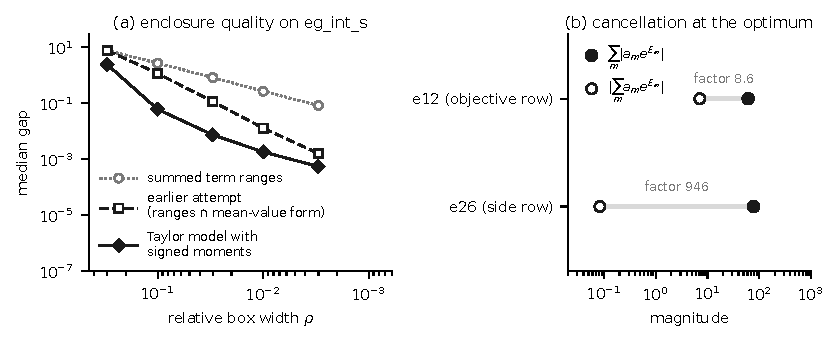
\includegraphics[width=\textwidth]{fig-eg-enclosures.pdf}
\caption{(a) Median gap between the sampled minimum of a row over a box and three lower bounds, against relative box width, over 64 boxes and 24 rows of \inst{eg_int_s} (numerical evidence). (b) Cancellation at our best point of \inst{eg_int_s}: sum of absolute values of the 97 kernel terms against the absolute value of their sum, for the active objective row e12 and the Gaussian part of the active side row e26.}
\label{fig:eg-enclosures}
\end{figure}

\subsubsection{Exactly feasible points}\label{app:eg-primal}

\Cref{tab:eg-points} lists the points.
The decision variables are the shortest round-trip decimal strings of binary64 search points, read as exact decimals, and $x_{\mathrm{obj}}$ is a 20-digit decimal obtained by rounding up a high-precision evaluation of $\Phi$.
The objective of the point is $x_{\mathrm{obj}}$ itself, so $\Uprim_I$ is this decimal; \cref{tab:closures} displays it rounded up.

\begin{table}[ht]
\centering
\footnotesize
\setlength{\tabcolsep}{3pt}
\caption{Exactly feasible points (decimal strings read as exact rationals).}
\label{tab:eg-points}
\begin{tabular}{@{}lll>{\raggedright\arraybackslash}p{6.5cm}@{}}
\toprule
instance & $x_{\mathrm{obj}}=\Uprim_I$ & integer coordinates & continuous coordinates\\
\midrule
\inst{eg_int_s} & 6.4531031593842274088 & $(x_5,x_6,x_7)=(2,4,3)$ & $(x_1,\dots,x_4)=(0.564219345763436$, $0.6468471890552644$, $1.0$, $0.9390699678023392)$\\
\inst{eg_disc_s} & 5.7605396164535106058 & $(x_1,\dots,x_4)=(3,10,8,12)$ & $(x_5,x_6,x_7)=(1.0800209145804143$, $3.485358811359775$, $2.2415838244871797)$\\
\inst{eg_disc2_s} & 5.6421005799711067563 & $(x_5,x_6,x_7)=(11,34,24)$ & $(x_1,\dots,x_4)=(0.339986187975027$, $1.0$, $0.7526242429543005$, $1.2370734367691458)$\\
\bottomrule
\end{tabular}
\end{table}

All bounds and integrality conditions hold exactly.
A library-free evaluation in dyadic interval arithmetic with its own OSIL reader (\cref{app:points-instances}) proves all 28 rows, with enclosure widths below $10^{-73}$, so the primal claims do not depend on mpmath; tests of its logarithm support, and do not replace, its alternating-series proof.
The smallest proved slacks of the objective rows, $\sci{5.57}{-20}$ (e12), $\sci{7.80}{-20}$ (e12) and $\sci{7.49}{-20}$ (e10), come from rounding $x_{\mathrm{obj}}$ up; the smallest side-row slacks are $\sci{1.49}{-11}$ (e26 of \inst{eg_int_s}, the row into whose interior the point was pushed), 0.140 and 0.123 (e25).

Under \cref{hyp:fp-ieee} and the correctness of the interval-mode implementation and its reader, the interval mode of the search proves the binary64 search points feasible with $\Phi$ at most $\Uprim'_I=6.4531031593862185$, $5.760539616455533$ and $5.642100579973559$.
Measured against these values the relative gaps are at most $\sci{1.00000008}{-9}$; against $\Uprim_I$ they are at most $\sci{9.997}{-10}$.
MINLPLib's listed points p1 of \inst{eg_int_s} and \inst{eg_disc_s} are feasible only within a tolerance: in a 60-digit evaluation, the first violates row e26 by $\sci{2.89}{-16}$ and, with its listed objective value, row e12 by $\sci{4.57}{-15}$, and the second violates row e12 by $\sci{1.66}{-14}$.
We do not use the listed points.

\subsubsection{Proof of \texorpdfstring{\cref{thm:eg-bounds}}{the eg theorem}}\label{app:eg-proof}

\begin{proof}[Proof of \cref{thm:eg-bounds}]
\emph{Dual bounds.}
Under the hypotheses of \cref{thm:eg-bounds}, \cref{thm:eg-trust} gives $\vstar(\model_I)\ge\theta^*_I\ge\Lcert_I$, from the coverage checks above, \cref{lem:eg-padding,lem:eg-boxtests,lem:eg-cover} and the audit.

\emph{Primal bounds.}
The points of \cref{tab:eg-points} are exactly feasible, and their objective values are $\Uprim_I$, so $\vstar(\model_I)\le\Uprim_I$.
The exact values of $\Lcert_I$ and $\Uprim_I$ give $\gapabs\le\sci{6.46}{-9}$, $\sci{5.76}{-9}$ and $\sci{5.64}{-9}$, and $\gaprel\le\sci{9.997}{-10}$ for all three.
\end{proof}

\Cref{tab:eg-matrix} records which certificate covers which part of each domain; the leaf re-certifier carries the displayed bounds.
The first implementation, the search that proposed the leaves, also certifies on its own, in outward-rounded interval arithmetic without library functions (its interval mode, under \cref{hyp:fp-ieee} and the correctness of its code), the bounds $6.4531031529331155383\ldots$ for \inst{eg_int_s} and $5.7605396106949937618\ldots$ for \inst{eg_disc_s}, and $5.6421005743314580627\ldots$ for the part of \inst{eg_disc2_s} with $x_7\in[24,27]$, all binary64 numbers above the displayed bounds.
The last holds under a side condition on its LP multipliers: that replay ran before a guard was added that rejects LP multiplier vectors whose objective weights do not have a positive sum, so it assumes that no such vector occurred.
LP duality makes these weights sum to 1, and the guarded rerun of the fast mode on that part saw a smallest sum of 0.9999999999999998, so we expect the condition to hold, but the replay did not log it.
The fast mode covers all parts but serves only as a cross-check, because its error analysis is not in paper form and it uses a library power function.
For parts 0 and 2--7 of \inst{eg_disc2_s}, a separately written outward-rounded interval certifier without library functions also re-certified 10{,}404 leaves (the 300 with the smallest margins, 1{,}000 random leaves and the 200 with the smallest lower bounds of each part; 117{,}214 pieces; no failure).

\begin{table}[ht]
\centering
\footnotesize
\setlength{\tabcolsep}{4pt}
\caption{Certificates by part of the domain.
``All'' means every leaf of the part.
Trust bases: leaf re-certifier with audit, \cref{thm:eg-trust}; interval mode, \cref{hyp:fp-ieee} and its code; fast mode, an unpublished error analysis and a library power function (cross-check only).
$^\dagger$Under the side condition on the LP multipliers stated in the text.}
\label{tab:eg-matrix}
\begin{tabular}{@{}lrllll@{}}
\toprule
part & leaves & re-certifier & interval mode & fast mode & interval sample\\
\midrule
\inst{eg_int_s} & 33{,}385 & all & complete & complete & ---\\
\inst{eg_disc_s}, $x_4\in[7,11]$ & 46{,}223 & all & complete & complete & ---\\
\inst{eg_disc_s}, $x_4\in[12,15]$ & 40{,}573 & all & complete & complete & ---\\
\inst{eg_disc2_s}, $x_7\in[24,27]$ & 135{,}317 & all & complete$^\dagger$ & complete & ---\\
\inst{eg_disc2_s}, other 7 parts & 979{,}044 & all & --- & complete & 10{,}404 leaves\\
\bottomrule
\end{tabular}
\end{table}

% Plan: development/outline.md, section 6, item B.8.
% Sources: development/dossiers/waterno2.md and waterno2.critique.md; run
% times as in Section 10 (R/publication/reproduction/water-audit/logs/
% vbb2_*.time: 63 runs, 26,809 s wall; certB re-bounding 214,979 CPU-s on a
% loaded machine, critique C2 for the unloaded estimate).
\subsection{The \inst{waterno2} instances}\label{app:waterno2}

The proof of \cref{thm:waterno2-bounds} combines a period Lagrangian (\cref{prop:waterno2-lagrangian}; \inst{waterno2_09}--\inst{waterno2_24}) or cellwise slopes (\cref{prop:waterno2-cells}; \inst{waterno2_06}) with a finite list of statements ``this period or pair problem has infimum at least~$b$'', each established by two separately written rigorous branch-and-bound codes (\cref{lem:waterno2-bb}).

\subsubsection{Model}\label{app:waterno2-model}

The network is n9p3a11 of \citet[Section~5.5]{huang2019-optimal-operation-of-water-supply}: the four pump-power coefficients of its Example~5.41 occur exactly $2T$ times in each file \inst{waterno2_T}.
Water flows from a source through station~A (3 pumps) into tank~1, through parallel stations B1 and B2 (2 pumps each) into tank~2, and through station~D (2 pumps) into tank~3, which serves the demand.
The pumps of a station share one speed and one head; \inst{waterno2_T} covers $T$ periods of one hour.

Periods are $t=0,\dots,T-1$, and $w:=(1800,720,1600)/3600=(\tfrac12,\tfrac15,\tfrac49)$ collects the tank areas divided by 3600.
In period~$t$, pump~$p$ of station~$S$ has an on/off variable $y_{t,p}$, a flow $q_{t,p}$, a head $\eta_{t,p}$ and a cost $\gamma_{t,p}$; station~$S$ has a flow $Q_{t,S}=\sum_{p\in S}q_{t,p}$ (with $Q_{t,B}=Q_{t,B1}+Q_{t,B2}$), a speed $\omega_{t,S}$ and a head $H_{t,S}$.
The tank levels at the start and end of the period are $s_t,e_t\in\R^3$, and $h_t$ is a copy of $Q_{t,A}$.
Every monomial ($q^2$, $q^3$, $\omega^2$, $\omega^3$, $q\omega$, $q\omega^2$, $q^2\omega$, $y\omega^3$, $Q^2$) is an auxiliary variable defined by an equality row, and a few redundant auxiliaries occur.
With the balance rows divided by 3600, the OSIL model reads
\begin{equation}\label{eq:waterno2-model}
\begin{aligned}
\min\ & \textstyle\sum_{t}\sum_{p}\gamma_{t,p}\\
\text{s.t. }& q^{\min}_S y_{t,p}\le q_{t,p}\le q^{\max}_S y_{t,p},\qquad y_{t,p_1(S)}\ge y_{t,p_2(S)}\ (\ge y_{t,p_3(S)}),\\
& \omega^{\min}_S\le\omega_{t,S}\le\min\{1,\ \omega^{\min}_S+(1-\omega^{\min}_S)\,y_{t,p_1(S)}\},\\
& \eta_{t,p}=a_S\omega_{t,S}^2+b_S\,q_{t,p}\omega_{t,S}+c_S\,q_{t,p}^2,\\
& -2000\,(1-y_{t,p})\le\eta_{t,p}-H_{t,S}\le M_S\,(1-y_{t,p}),\\
& H_{t,A}=s_{t,1}+11+5Q_{t,A}^2,\qquad H_{t,D}=s_{t,3}-s_{t,2}+13+5Q_{t,D}^2,\\
& H_{t,B}=\zeta_t-s_{t,1}-60+4Q_{t,B}^2,\qquad \zeta_t\ge s_{t,2}+90,\\
& \kappa_t\,\gamma_{t,p}\ge P_S(y_{t,p},\omega_{t,S},q_{t,p}),\qquad \gamma_{t,p}\le\bar\gamma_{S,t},\\
& w_1(e_{t,1}-s_{t,1})=Q_{t,A}-Q_{t,B},\qquad w_2(e_{t,2}-s_{t,2})=Q_{t,B}-Q_{t,D},\\
& w_3(e_{t,3}-s_{t,3})=Q_{t,D}-d_t,\qquad s_t,e_t\in[2,5]\times[2.5,5]\times[2,6],\qquad s_0=\sigma:=(3.5,\,4.1,\,4),\\
& s_{t+1}=e_t\ \ (t=0,\dots,T-2),\qquad \textstyle\sum_t h_t\ge r_T,
\end{aligned}
\end{equation}
where $p_1(S),p_2(S),\dots$ are the pumps of~$S$ in order, $P_S$ is a cubic power polynomial, $\kappa_t$ is a tariff factor and the demand $d_t$ is fixed by a single-variable row.
All station data are exact decimals; for station~D, which the proofs below use,
\[
[q^{\min},q^{\max}]=[0.24,0.58],\quad \omega^{\min}=0.7,\quad (a,b,c)=(34.92732674,\,2.03724124,\,-63.61644904).
\]
In \inst{waterno2_06} the periods differ only in the demands
\[
d=(0.296666667,\ 0.294444444,\ 0.283888889,\ 0.277222222,\ 0.293333333,\ 0.306944444).
\]
For every $T$ the right-hand side $r_T$ of the horizon row (\cref{sec:split-waterno2}) satisfies $r_T=\sum_t d_t$ exactly, for example $r_6=1.752499999$.
All five instances minimize, and every row is a polynomial of degree at most~3.

At a switched-off station the speed equals $\omega^{\min}_S$, and the square and cube variables sit at their lower bounds $(\omega^{\min}_S)^2$ and $(\omega^{\min}_S)^3$; under the decimal semantics of \cref{sec:semantics-model} these are identities.
For binary64 data the speed of a switched-off station is $\fl(\omega^{\min}_S)$, and $\fl(\omega^{\min}_S)^2<\fl((\omega^{\min}_S)^2)$ and $\fl(\omega^{\min}_S)^3<\fl((\omega^{\min}_S)^3)$ for $\omega^{\min}_S\in\{0.6,0.85,0.7\}$ (for $0.8$ both inequalities are reversed).
So under \reading{c} no point with station A, B2 or D switched off in some period is feasible.
Beyond this, we claim nothing for \reading{c}.
The cube residual of the $0.7$ station, $\fl(0.7)^3-\fl(0.343)<-9.2\cdot10^{-17}$, triggers the wrong SCIP results of \cref{sec:solvers-invalid}.

\subsubsection{Period structure and the period Lagrangian}\label{app:waterno2-lagrangian}

Write $x=(x_0,\dots,x_{T-1})$ with $x_t\in\R^{166}$ the variables of period~$t$, and $s_t(x_t)$, $e_t(x_t)$, $h_t(x_t)$ for its start levels, end levels and horizon copy.
Let $C_t(x_t)$ be the sum of the nine cost variables of period~$t$, and $X_t$ the set of $x_t$ that satisfy the 203 rows of period~$t$, the bounds of its variables and integrality.

\begin{lemma}[period structure]\label{lem:waterno2-structure}
In each model, every row other than the horizon row and the $3(T-1)$ link rows $s_{t+1,k}=e_{t,k}$ involves variables of one period only; each period has 166 variables (9 binary) and 203 rows, and the objective is $\sum_tC_t(x_t)$.
\end{lemma}

\begin{proof}
This is a finite property of the row--variable incidence.
Three separately written programs recover it for all five files; one orients each link row by the sign of the area coefficient and orders the periods along the chain of link rows.
In \inst{waterno2_06} the link rows are \texttt{e111}--\texttt{e125} and the horizon row is \texttt{e56}.
\end{proof}

The certificates also use valid boxes: if $I_t\subset\R^{166}$ is a box that contains $x_t$ for every $x\in\feas$, then $X'_t:=X_t\cap I_t$ can replace $X_t$ without changing the feasible set.
Each implementation below uses its own file of such boxes, proved by outward-rounded or exact feasibility-based and optimization-based bound tightening (FBBT, OBBT) on the model without the horizon row, which is a relaxation of~$\model$.

\begin{proposition}[period Lagrangian]\label{prop:waterno2-lagrangian}
Let $\lambda_0,\dots,\lambda_{T-2}\in\R^3$, $\mu\ge0$ and $\lambda_{-1}=\lambda_{T-1}=0$, and let
\[
\varphi_t(\lambda,\mu)=\inf\bigl\{C_t(x_t)+\lambda_{t-1}^{\top}s_t(x_t)-\lambda_t^{\top}e_t(x_t)-\mu\,h_t(x_t):\ x_t\in X'_t\bigr\}.
\]
Then $\vstar(\model)\ge\mu r_T+\sum_t\varphi_t(\lambda,\mu)\ge\mu r_T+\sum_tB_t$ for any numbers $B_t\le\varphi_t(\lambda,\mu)$.
\end{proposition}

\begin{proof}
Let $x\in\feas$ (if there is none, $\vstar=+\infty$).
The link rows give $\sum_{t\le T-2}\lambda_t^{\top}(s_{t+1}(x_{t+1})-e_t(x_t))=0$, and the horizon row with $\mu\ge0$ gives $\mu(r_T-\sum_th_t(x_t))\le0$.
Adding both to the objective and grouping by period,
$\sum_tC_t(x_t)\ge\mu r_T+\sum_t[C_t+\lambda_{t-1}^{\top}s_t-\lambda_t^{\top}e_t-\mu h_t](x_t)\ge\mu r_T+\sum_t\varphi_t(\lambda,\mu)$, since $x_t\in X'_t$ by \cref{lem:waterno2-structure}.
\end{proof}

Any binary64 multipliers with $\mu\ge0$, read as exact rationals, give a valid bound; ours came from a bundle method that used SCIP as an untrusted oracle.
No variable receives two Lagrangian terms, so every objective coefficient of a period problem is a binary64 number.

\begin{lemma}[the horizon row is a terminal-volume row]\label{lem:waterno2-horizon}
Every $x$ that satisfies the balance, copy, link and demand rows of \eqref{eq:waterno2-model} and the fixed initial levels $s_0=\sigma$ satisfies $\sum_th_t(x)-\sum_td_t=w^{\top}(e_{T-1}(x)-\sigma)$.
Since $r_T=\sum_td_t$, such an $x$ satisfies the horizon row if and only if $w^{\top}e_{T-1}\ge w^{\top}\sigma=\tfrac{3913}{900}$, that is, $1800\,e_{T-1,1}+720\,e_{T-1,2}+1600\,e_{T-1,3}\ge15652$.
\end{lemma}

\begin{proof}
After merging copies, the balance rows of period~$t$ read $w_1(e_{t,1}-s_{t,1})=h_t-Q_{t,B}$, $w_2(e_{t,2}-s_{t,2})=Q_{t,B}-Q_{t,D}$ and $w_3(e_{t,3}-s_{t,3})=Q_{t,D}-d_t$; their sum is $w^{\top}(e_t-s_t)=h_t-d_t$.
Summing over~$t$ with $s_{t+1}=e_t$ and $s_0=\sigma$ telescopes to the identity, and $w^{\top}\sigma=\tfrac12\cdot3.5+\tfrac15\cdot4.1+\tfrac49\cdot4=\tfrac{3913}{900}$.
\end{proof}

Three separate derivations checked the identity $r_T=\sum_td_t$ in exact arithmetic for all horizons.

\begin{remark}[folding the horizon multiplier]\label{rem:waterno2-folding}
For $x$ as in \cref{lem:waterno2-horizon} but without the link rows, $\mu(r_T-\sum_th_t)=\mu w^{\top}(\sigma-e_{T-1})+\sum_{t\le T-2}\mu w^{\top}(s_{t+1}-e_t)$.
A horizon multiplier thus shifts every link slope by $\mu w$ and adds a price on the final volume that is nonpositive under the terminal row; imposing the terminal row in the last period, setting $\mu=0$ and using the slopes $\lambda_t+\mu w$ gives a bound at least as large as \cref{prop:waterno2-lagrangian}.
\end{remark}

\subsubsection{Cells, slopes and a shortest path}\label{app:waterno2-cells}

A period's value is nonconvex in its boundary levels (heads depend on the start levels, and pumps switch with minimum flows), so under linear prices one period may end at one level vector while the next starts at another.
Cells with their own slope vectors make such jumps unprofitable.
Let $Y_l=\{e_l(x):x\in\feas\}\subset\R^3$ for $l=0,\dots,T-2$.

\begin{proposition}[cellwise slopes]\label{prop:waterno2-cells}
Assume:
(a) each $\mathcal P_l$ is a finite family of closed boxes (cells) with $Y_l\subseteq\bigcup\mathcal P_l$;
(b) each cell $D\in\mathcal P_l$ carries one vector $\lambda_{l,D}\in\R^3$;
(c) for every period~$t$ and pair $(D,D')\in\mathcal P_{t-1}\times\mathcal P_t$, the number $b_t(D,D')\in\R\cup\{+\infty\}$ satisfies $b_t(D,D')\le\varphi_t(D,D')$, where
\[
\varphi_t(D,D')=\inf\bigl\{C_t(x_t)+\lambda_{t-1,D}^{\top}s_t(x_t)-\lambda_{t,D'}^{\top}e_t(x_t):\ x_t\in X'_t,\ s_t(x_t)\in D,\ e_t(x_t)\in D'\bigr\},
\]
with the terminal row of \cref{lem:waterno2-horizon} added for $t=T-1$, $\inf\emptyset=+\infty$, no entry cell or term for $t=0$ and no exit cell or term for $t=T-1$.
Then $\vstar(\model)\ge V:=\min_{(D_0,\dots,D_{T-2})}\sum_{t=0}^{T-1}b_t(D_{t-1},D_t)$, the length of a shortest path in the layered graph with arc weights~$b_t$; if $V=+\infty$, then $\feas=\emptyset$.
\end{proposition}

\begin{proof}
Let $x\in\feas$.
By~(a) choose $D_l\in\mathcal P_l$ containing $e_l(x)=s_{l+1}(x)$, and let both periods adjacent to link~$l$ use it.
The link rows give $\sum_l\lambda_{l,D_l}^{\top}(s_{l+1}(x)-e_l(x))=0$, so
$\sum_tC_t(x_t)=\sum_t[C_t(x_t)+\lambda_{t-1,D_{t-1}}^{\top}s_t(x_t)-\lambda_{t,D_t}^{\top}e_t(x_t)]$.
Since $x_t\in X'_t$, $s_t(x_t)\in D_{t-1}$, $e_t(x_t)\in D_t$, and the terminal row holds by \cref{lem:waterno2-horizon}, the $t$-th term is at least $\varphi_t(D_{t-1},D_t)\ge b_t(D_{t-1},D_t)$; the sum is the length of a path, hence at least~$V$.
\end{proof}

This is the path case of \cref{prop:split-cellwise}: the exit term of period~$l$ and the entry term of period~$l+1$ use the same $\lambda_{l,D}$, so slopes may jump across cell faces but may not depend on the other cell of a pair.
With one cell per link and slopes $\lambda_t+\mu w$, the proposition is at least as strong as \cref{prop:waterno2-lagrangian} (\cref{rem:waterno2-folding}).
Lagrangian decomposition of multi-period pump scheduling is the subject of \citet{ghaddar2015-a-lagrangian-decomposition-approach-for}, which we could not read (\cref{app:literature}).
Pump scheduling has other global-optimization precedents, such as the polyhedral relaxations of \citet{tasseff2022-polyhedral-relaxations-for-optimal-pump}.
We claim no novelty for period decomposition or for cellwise slopes.

\begin{lemma}[reusing a bound after a slope change]\label{lem:waterno2-reuse}
Let $B_r\in\R\cup\{+\infty\}$ satisfy $B_r\le\inf\{C_t+a^{\top}s_t-a'^{\top}e_t:\ x_t\in X'_t,\ s_t\in A_{\mathrm{in}},\ e_t\in A_{\mathrm{out}}\}$ for boxes $A_{\mathrm{in}},A_{\mathrm{out}}$ and slopes $a,a'$ (with the terminal row if $t=T-1$).
If $D=[\ell,\upsilon]\subseteq A_{\mathrm{in}}$ and $D'=[\ell',\upsilon']\subseteq A_{\mathrm{out}}$ carry slopes $l=\lambda_{t-1,D}$ and $l'=\lambda_{t,D'}$, then
\[
\varphi_t(D,D')\ \ge\ B_r+\sum_{k=1}^3\min\{(l_k-a_k)\ell_k,\ (l_k-a_k)\upsilon_k\}+\sum_{k=1}^3\min\{-(l'_k-a'_k)\ell'_k,\ -(l'_k-a'_k)\upsilon'_k\},
\]
and $B_r=+\infty$ implies $\varphi_t(D,D')=+\infty$.
For $t=0$ the entry boxes, slopes and terms are absent, and for $t=T-1$ the exit ones.
\end{lemma}

\begin{proof}
The feasible set of $(D,D')$ is contained in that of $(A_{\mathrm{in}},A_{\mathrm{out}})$; on it the pair objective equals the record objective plus $(l-a)^{\top}s_t-(l'-a')^{\top}e_t$, whose minimum over a box is attained coordinatewise at end points.
\end{proof}

Condition~(a) needs ranges for the link levels; for \inst{waterno2_06} the next lemma derives them from the rows.

\begin{lemma}[level ranges at the links of \inst{waterno2_06}]\label{lem:waterno2-levels}
Every exactly feasible point of \inst{waterno2_06} satisfies
(a) $e_{0,3}\ge3.33249999925$, $e_{1,3}\ge2.67000000025$ and $e_{2,3}\ge2.03125$;
(b) $e_{0,3}\le5.6976271$; and
(c) $e_l\in[2,5]\times[2.5,5]\times[2,6]$ for every link~$l$.
\end{lemma}

\begin{proof}
Part~(c) is the OSIL box of the levels.
(a) The tank-3 balance gives $e_{t,3}=s_{t,3}+\tfrac94(Q_{t,D}-d_t)$ with $Q_{t,D}\ge0$.
From $s_{0,3}=4$ and $s_{t+1,3}=e_{t,3}$:
$e_{0,3}\ge4-\tfrac94\cdot0.296666667=3.33249999925$,
$e_{1,3}\ge3.33249999925-\tfrac94\cdot0.294444444=2.67000000025$ and
$e_{2,3}\ge2.67000000025-\tfrac94\cdot0.283888889=2.03125$.

(b) In period~0, $s_{0,2}=4.1$ and $s_{0,3}=4$ are fixed, so $H_{0,D}=12.9+5Q_{0,D}^2$.
The two D pumps share $\omega\in[0.7,1]$ and $H_{0,D}$, and for a running pump the big-$M$ rows force $\eta=H_{0,D}$, so its flow satisfies $c\,q^2+b\,\omega q+(a\omega^2-H_{0,D})=0$ with the station-D coefficients $a,b>0>c$ given above.
If the first pump is off, the symmetry row switches the second off and $Q_{0,D}=0$.
If exactly one runs, $Q_{0,D}=q\le0.58$.
If both run with different flows, these are the two roots of the quadratic, whose sum $-b\omega/c\le2.03724124/63.61644904<0.0321$ contradicts the minimum flows ($2\cdot0.24$).
If both run with the same flow~$q$, then $Q_{0,D}=2q$, $H_{0,D}=12.9+20q^2$ and, using $0\le\omega\le1$ and $q\ge0$,
$83.61644904\,q^2=a\omega^2+b\,q\omega-12.9\le22.02732674+2.03724124\,q$.
The quadratic $83.61644904\,q^2-2.03724124\,q-22.02732674$ is positive at $q=0.5255838$ and increasing beyond, so $Q_{0,D}=2q\le1.0511676$.
In all cases $e_{0,3}=4+\tfrac94(Q_{0,D}-0.296666667)\le5.69762709925$.
\end{proof}

Part~(b) uses the period-0 rows \texttt{e44}, \texttt{e50} (pump curves), \texttt{e75}, \texttt{e516} (station flow), \texttt{e81} (demand), \texttt{e105} (balance), \texttt{e168}, \texttt{e174}, \texttt{e222}, \texttt{e228} (flow ranges), \texttt{e240}, \texttt{e246}, \texttt{e264}, \texttt{e282}, \texttt{e720}, \texttt{e721} (head of~D), \texttt{e468} (speed), \texttt{e498} (symmetry), \texttt{e564}, \texttt{e570}, \texttt{e618}, \texttt{e624} (big-$M$), the monomial rows \texttt{e900}, \texttt{e901}, \texttt{e924}, \texttt{e925}, \texttt{e1170}, \texttt{e1172}, \texttt{e1174}, \texttt{e1175}, the fixed levels $\texttt{x254}=4.1$ and $\texttt{x266}=4$, and the bounds $0.7\le\texttt{x542}\le1$ of the speed; all arithmetic was checked in exact rationals.

\subsubsection{Rigorous bounds for the period and pair problems}\label{app:waterno2-bb}

With the monomials replaced by auxiliary variables, a period or pair problem minimizes a linear function $c^{\top}z$ over a set $S$ defined by polynomial rows of degree at most~3, bounds and integrality.

\begin{lemma}[branch-and-bound soundness]\label{lem:waterno2-bb}
Let $\tau\in\R$, and let $N$ be a finite list of boxes such that every $z\in S$ with $c^{\top}z<\tau$ lies in a box of~$N$, each $\beta\in N$ carrying a number $b(\beta)\le\inf\{c^{\top}z:z\in S\cap\beta\}$.
Then $\inf_Sc^{\top}z\ge\min\{\tau,\min_{\beta\in N}b(\beta)\}$ (with $\min\emptyset=+\infty$).
The hypothesis holds for $N=\{\beta_0\}$ with $\beta_0\supseteq S$ and is preserved by
(i) splitting a box into two closed boxes whose union is the box;
(ii) shrinking $\beta$ to a box containing $\{z\in S\cap\beta:c^{\top}z<\tau\}$, which covers outward-rounded FBBT, OBBT with or without the cutoff $c^{\top}z\le\tau$, and reduced-cost tightening; and
(iii) deleting $\beta$ when $b(\beta)\ge\tau$ or when $S\cap\beta=\emptyset$ is proved.
\end{lemma}

\begin{proof}
A point $z\in S$ has $c^{\top}z\ge\tau$ or lies in some $\beta\in N$, where $c^{\top}z\ge b(\beta)$; operations (i)--(iii) keep every $z\in S$ with $c^{\top}z<\tau$ in the union of the list.
\end{proof}

Both codes return $+\infty$ only when root propagation or root OBBT, both without cutoff, proves the root box infeasible, so that $S=\emptyset$; emptiness found inside the tree only closes a box.
Node bounds come from a linear relaxation on the box $[\ell,\upsilon]$: tangents and the secant of $w=x^2$; for $w=x^3$ with $x\ge0$, tangents $w\ge3p^2x-2p^3$ ($p\ge0$; $x^3-3p^2x+2p^3=(x-p)^2(x+2p)$) and the secant $w\le(\ell^2+\ell\upsilon+\upsilon^2)x-\ell\upsilon(\ell+\upsilon)$ (the difference is $(x-\ell)(x-\upsilon)(x+\ell+\upsilon)\le0$); and McCormick inequalities for products, including binary times continuous.
For relaxation rows $A_Iz\le b_I$, $A_Ez=b_E$ and any $y$ with $y_I\ge0$,
\begin{equation}\label{eq:waterno2-safe}
\min\{c^{\top}z:\ A_Iz\le b_I,\ A_Ez=b_E,\ \ell\le z\le\upsilon\}\ \ge\ -y^{\top}b+\sum_j\min\{(c+A^{\top}y)_j\ell_j,\ (c+A^{\top}y)_j\upsilon_j\},
\end{equation}
because $c^{\top}z\ge c^{\top}z+y^{\top}(Az-b)$ for every feasible~$z$ \citep{neumaier2004-safe-bounds-in-linear-and}.
HiGHS supplies~$y$; a poor~$y$ only weakens the bound.

The first implementation (code~P) was written together with the certificates.
It encloses every decimal in $[\mathrm{down}(v),\mathrm{up}(v)]$, propagates in binary64 with one \texttt{nextafter} step outward per operation and a padding of $10^{-12}\sum|\text{terms}|$ for every sum of $n\le9000$ terms (which exceeds $\gamma_{n-1}\sum|\text{terms}|$), evaluates \eqref{eq:waterno2-safe} with outward-rounded interval coefficients, and also uses reduced-cost tightening and root OBBT with cutoff.
The second (code~V) was written later, in separate agent sessions, reads exact rationals and evaluates \eqref{eq:waterno2-safe} in exact rational arithmetic.
Its two variants share the model builder, relaxation and node bound: V$_{\mathrm{ex}}$ propagates in exact rational arithmetic, and V$_{\mathrm{fl}}$, whose propagation a later session added, in binary64 with one outward step per $\times$, $\div$ and $\sqrt{\ }$, sums by Python's correctly rounded \texttt{math.fsum} plus two steps, and cubes and cube roots checked exactly.
V$_{\mathrm{fl}}$'s propagation agreed with V$_{\mathrm{ex}}$'s in 3,000 compared passes and was read by a separate agent session, but it is not proved correct.

\subsubsection{Proof of \texorpdfstring{\cref{thm:waterno2-bounds}}{the waterno2 theorem}}\label{app:waterno2-proof}

\emph{$T\in\{9,12,18,24\}$.}
The archive stores binary64 multipliers $\lambda$ and $\mu\ge0$ and one number $B_t$ per period.
For each of the 63 periods, code~P and code~V$_{\mathrm{fl}}$ each established $B_t\le\varphi_t(\lambda,\mu)$ by \cref{lem:waterno2-bb} with target~$B_t$ and their own valid boxes.
\Cref{prop:waterno2-lagrangian} gives $\vstar\ge\mu r_T+\sum_tB_t$, evaluated in exact rational arithmetic by three implementations (\cref{tab:waterno2-values}).

\emph{$T=6$.}
The certificate applies \cref{prop:waterno2-cells} with $\mu=0$ and the terminal row in period~5.
For links $l=0,\dots,4$, split trees partition root boxes $[2,5]\times[2.5,5]\times J_l$ into $228$, $154$, $148$, $153$ and $240$ cells, with $J_0=[3.3324999992334576,\ 5.936197237759838]$, $J_1=[2.6700000002022537,\ 6]$, $J_2=[2.0312499999222715,\ 6]$ and $J_3=J_4=[2,6]$ (binary64 end points).
By \cref{lem:waterno2-levels} each root box contains~$Y_l$.
The leaves lie in the root, have pairwise disjoint interiors and total volume equal to the root's (checked exactly), so their union is a closed subset of the root of full measure, hence the whole root box, and~(a) holds.
Each leaf carries one binary64 slope vector, used by both adjacent periods ($101$, $130$, $135$, $139$ and $174$ distinct vectors per link), so~(b) holds.
The archive stores $77{,}249$ records (a period, two boxes, two slope vectors and a claimed bound $B_r$ in the sense of \cref{lem:waterno2-reuse}), of which $49{,}315$ are used.
For each of the $117{,}736$ leaf pairs, $b_t(D,D')$ is the largest bound \cref{lem:waterno2-reuse} gives over the records of period~$t$ whose boxes contain $D$ and~$D'$, so~(c) holds given the record statements.
The table has $79{,}919$ finite pair bounds ($52{,}826$ with a nonzero correction) and $37{,}817$ pairs proved empty.
Code~P and code~V$_{\mathrm{fl}}$ each established every one of the $49{,}315$ record statements.
The shortest path, computed in exact rational arithmetic and recomputed by two further implementations, is $V=39157472136693483/2^{47}=278.2305737745\ldots$.

\emph{Primal values.}
The values~$\Uprim$ in \cref{tab:unclosed} are objective values of exactly feasible points whose coordinates lie in~$\Q$ or in one quadratic field each; three exact checkers decide every row, bound and integrality requirement (\cref{app:points}).
The \inst{waterno2_06} point is MINLPLib's listed point~p4 made exactly feasible; the other four points are ours and improve the listed primal values by at least $8.58$, $29.53$, $245.65$ and $368.92$.
Since $0<\Lcert<\Uprim$, $\gaprel=(\Uprim-\Lcert)/\Lcert$.
\qed

\begin{table}[t]
\centering\small
\caption{Exact values of the \inst{waterno2} dual bounds and their displays (rounded down): $V$ of \cref{prop:waterno2-cells} for \inst{waterno2_06}, and $\mu r_T+\sum_tB_t$ of \cref{prop:waterno2-lagrangian} otherwise. Nodes: branch-and-bound nodes of code~P over all periods.}
\label{tab:waterno2-values}
\begin{tabular}{@{}llll@{}}
\toprule
instance & exact value & display & computed statements\\
\midrule
\inst{waterno2_06} & $39157472136693483/2^{47}$ & $278.230573$ & $49{,}315$ records\\
\inst{waterno2_09} & $3627661341387654598825371/(2^{42}\cdot10^{9})$ & $824.834692$ & 9 periods, $108{,}519$ nodes\\
\inst{waterno2_12} & $9190837775594918144252281/(2^{42}\cdot10^{9})$ & $2089.754565$ & 12 periods, $140{,}952$ nodes\\
\inst{waterno2_18} & $5267563083146225483626937/(2^{40}\cdot10^{9})$ & $4790.820715$ & 18 periods, $381{,}084$ nodes\\
\inst{waterno2_24} & $115688878681251187594323079/(2^{44}\cdot10^{9})$ & $6576.151388$ & 24 periods, $525{,}224$ nodes\\
\bottomrule
\end{tabular}
\end{table}

The intermediate \inst{waterno2_06} bound $272.584700$ of \cref{tab:unclosed} used one slope vector per link and $113$--$162$ cells per link.
Cells were then refined where the minimizing path jumped inside a cell, and slopes were tuned from small LPs over pools of SCIP points; these heuristics affect only the strength of the bound.

\subsubsection{Verification, trust base and regeneration}\label{app:waterno2-verification}

The two lines are separately written in the sense of \cref{sec:semantics-protocol}: code~V neither imports nor runs code~P in its checks.
The session that wrote V$_{\mathrm{fl}}$ imported code~P once, read-only, to compare the period objectives coefficient by coefficient; no certified value uses that comparison.
Code~P has its own model builder and valid boxes, which an exact FBBT/OBBT run of the second line reproduced or improved, while V$_{\mathrm{ex}}$ and V$_{\mathrm{fl}}$ share the second line's builder, relaxation and node bound.
A wrong value would require an error in both lines on the same statement, or in a shared component: the OSIL reader, rational arithmetic, IEEE binary64 arithmetic with correctly rounded square roots and \texttt{nextafter} (\cref{hyp:fp-ieee}), and, for V$_{\mathrm{fl}}$, Python's correctly rounded \texttt{math.fsum} (a further checking-program assumption, not part of \cref{hyp:fp-ieee}).
No library transcendental enters, since every row is polynomial.
SCIP and HiGHS supply only hints (multipliers, targets, slope proposals, dual vectors, branching points); no SCIP value enters a bound.
Necessary conditions hold: the exactly feasible points satisfy every file of valid boxes; at these points each of the 69 period-Lagrangian objectives is at least its~$B_t$, and each \inst{waterno2_06} period value is at least the pair bound of the leaves that contain the point; and the second line rejected deliberately unattainable targets.

The search trees are not stored, so the period and record statements can be re-established only by rerunning the searches; for fixed targets and a fixed software stack the searches are deterministic (identical status, bound and node count in repeated runs).
A checker for stored leaf certificates would have to re-verify every tightening step, so its cost is uncertain; we did not build one.
Regeneration derives each period target anew from time-limited SCIP runs and proves it with code~P; for \inst{waterno2_18} and \inst{waterno2_24} it gave slightly lower, also valid values (\cref{app:repro-regen}), and the values of \cref{thm:waterno2-bounds} rest on the original code-P run and the V$_{\mathrm{fl}}$ recheck at the stored targets.

\begin{certbox}[Certificate for \cref{thm:waterno2-bounds}]
\certitem{Inputs}{OSIL SHA-256 prefixes \texttt{3b0b316d7a9f} (06), \texttt{015932376b18} (09), \texttt{add485a67c22} (12), \texttt{968ff496844d} (18), \texttt{91d2612f435c} (24); multipliers and period bounds (09--24); split trees, leaf slopes and 77,249 records (06); valid-box files of both lines.}
\certitem{Computation}{63 period statements and 49,315 record statements by branch and bound (\cref{lem:waterno2-bb}), code~P in \arith{F} and code~V with \arith{E} node bounds; sums, cover check, corrections and shortest path in \arith{E}.}
\certitem{Data reading}{code~P: outward enclosure of each decimal; code~V: exact rationals; one shared OSIL reader, reproduced exactly by a separately written parser; the polynomial rows built by both codes equal an exact parse of the GAMS form, which separate exact parsers find identical to the OSIL form for all five instances.}
\certitem{Implementations}{code~P established every period and record statement. Second line: V$_{\mathrm{ex}}$ with its own valid boxes certified the six period statements of the \inst{waterno2_06} period Lagrangian ($263.735099$) at the same values; V$_{\mathrm{fl}}$ with its own valid boxes certified all 63 period statements of 09--24 (exact sums identical) and, with a separate driver and terminal row, the 49,315 used records of 06 (33,899 certified, 15,416 proved empty, among them all 12,298 with $B_r=+\infty$; none failed) and the 556 leaf pairs corrected by \cref{lem:waterno2-reuse}, at the leaf slopes (436 certified, 120 empty). Either line yields every displayed value. Sums, cover check, corrections and shortest path by the exact code and two further exact codes, with identical rationals.}
\certitem{Evidence level}{\evid{hand} for \cref{prop:waterno2-lagrangian,prop:waterno2-cells} and the lemmas; \evid{rerun} for the period and record statements.}
\certitem{Replay}{Tier~1 for the combination steps (seconds); for the period statements of 09--24 (7.4\,h in all, V$_{\mathrm{fl}}$), Tier~2 for 09 and 12 (35 and 49\,min) and Tier~3 for 18 and 24 (2.5 and 3.5\,h); Tier~3 for the record statements of 06 (about 60 CPU-hours on a loaded machine); \cref{app:repro}.}
\end{certbox}

% Plan: development/outline.md, section 6, item B.9.
% Sources: development/dossiers/ann-kan.md and ann-kan.critique.md;
% development/reviews/sol-kan-rigexp.md; ANN replay and verification times
% from R/publication/reproduction/network/logs/ann.*.time (replay user
% times 1,860 + 5,180 s; verification 1,159 + 5,234 + 924 s on two
% processes, 70.7 min elapsed), as in Section 10.
\subsection{\inst{ann_cumene_tanh} and the Kolmogorov--Arnold network (KAN) instances}\label{app:annkan}

Both families embed trained networks whose variables are determined by a few inputs, so the dual bounds come from branch and bound over the inputs.
\Cref{app:annkan-ann,app:annkan-ann-bb,app:annkan-ann-verif} prove \cref{thm:ann-bound}, and \cref{app:annkan-kan,app:annkan-kan-infeasible,app:annkan-kan-enclosure} prove \cref{prop:kan-infeasible,thm:kan-enclosure}.

\subsubsection{The model \texorpdfstring{\inst{ann_cumene_tanh}}{ann\_cumene\_tanh}}\label{app:annkan-ann}

The instance comes from \citet[Section~5.4]{schweidtmann2019-deterministic-global-optimization-with-artificial}: the operating point of a cumene process is optimized on a hybrid model of 14 multilayer perceptrons with tanh activations.
MINLPLib added it in 2021 in the source's full-space formulation.
It has 794 continuous variables and 790 rows (789 equalities) and minimizes \texttt{objvar}, the negative profit.
The inputs $u=(x_{723},\dots,x_{727})$ range over the box $\mathcal U=[360,390]\times[0.37,1]\times[1.31,1.97]\times[0.85,0.99]\times[0.2,1.2]$, and the inequality row \texttt{e789} is the purity requirement $x_{772}\ge0.999$.

In a suitable order, 529 linear rows and 250 rows $x_v=\tanh(x_s)$ each contain exactly one new variable, which enters linearly with a nonzero constant coefficient or as the left side of a tanh row.
They determine 779 variables as explicit functions $x(u)$, of which 722 have finite bounds, among them the training domain $[-1,1]$ of 70 normalized network inputs.
The remaining ten variables are free except \texttt{objvar} (bounds $\pm10^{20}$) and occur only in \texttt{e749}, \texttt{e750}, \texttt{e782}--\texttt{e788} and the objective row \texttt{e790}.
Rows \texttt{e782}--\texttt{e786} read $x_{746}x_w=\Pi_w$ for $w=x_{787},\dots,x_{791}$, with $\Pi_w$ quadratic in determined variables; \texttt{e787} reads $x_{765}x_{772}+x_{766}x_{792}=x_{760}x_{763}$ and \texttt{e788} reads $x_{792}+x_{793}=1$; and \texttt{e790} writes \texttt{objvar} as $c_0=10619.965999999999$ plus six linear terms in determined variables plus multiples of $x_{746}x_w$, $x_{766}x_{792}$ and $x_{766}x_{793}$.
Substituting the products gives
\[
\begin{aligned}
f(u)={}&c_0+\textstyle\sum_{j\in J}a_jx_j(u)+\sum_wc_w\Pi_w(x(u))\\
&+c_{92}\bigl(x_{760}x_{763}-x_{765}x_{772}\bigr)(u)+c_{93}\bigl(x_{766}-x_{760}x_{763}+x_{765}x_{772}\bigr)(u),
\end{aligned}
\]
and we bound $f$ over
\[
\Omega:=\bigl\{u\in\mathcal U:\ \ell_v\le x_v(u)\le\upsilon_v\ \text{for all 722 bounded determined }v,\ \ x_{772}(u)\ge0.999\bigr\}.
\]

\begin{lemma}[reduction]\label{lem:ann-reduction}
If $x$ is an exactly feasible point of \inst{ann_cumene_tanh} and $u=(x_{723},\dots,x_{727})$, then $u\in\Omega$, the determined coordinates of $x$ equal $x(u)$, and $\texttt{objvar}=f(u)$.
Hence $\vstar(\model_{\mathrm{ann}})\ge\inf_\Omega f$.
\end{lemma}

\begin{proof}
The forward rows determine the coordinates of~$x$ one by one, so they equal $x(u)$, and their bounds and \texttt{e789} are the constraints of~$\Omega$.
Rows \texttt{e782}--\texttt{e786} give $x_{746}x_w=\Pi_w(x(u))$, row \texttt{e787} gives $x_{766}x_{792}=x_{760}x_{763}-x_{765}x_{772}$, and row \texttt{e788} multiplied by $x_{766}$ gives $x_{766}x_{793}=x_{766}-x_{766}x_{792}$; substituting into \texttt{e790} yields $\texttt{objvar}=f(u)$.
No division is used, so points where $x_{746}$ or $x_{766}$ vanishes are covered.
\end{proof}

$\Omega$ drops \texttt{e749}, \texttt{e750}, the solvability of the product rows and the bound on \texttt{objvar}, so it may be larger than the projection of the feasible set.
MINLPLib's \inst{ann_cumene_exp} replaces $-\tanh(x_s)$ in each tanh row by $2/(\exp(2x_s)+1)-1$ and moves the constant into the row bounds; an exact comparison of the OSIL files shows that all other data coincide.
Since $\exp(2x_s)+1>0$, both models have the same feasible points and objective values, so \cref{thm:ann-bound} and the primal point hold verbatim for \inst{ann_cumene_exp}.
\Cref{app:literature} compares $\Omega$ with the reduced-space formulation of the source.

\subsubsection{Branch and bound over the inputs}\label{app:annkan-ann-bb}

The search starts from the outward binary64 enclosure of~$\mathcal U$.
It prunes a box~$Q$, bisects it at a binary64 point of one coordinate, or shrinks it by interval propagation to $Q_{\mathrm{red}}$ and records the removed part as at most ten slab boxes, so that $Q$ is the union of $Q_{\mathrm{red}}$ and the slabs.
It ran for 1800\,s from $\mathcal U$, and then for 5400\,s from the 111,474 boxes left open.

\begin{lemma}[covering]\label{lem:ann-cover}
$\mathcal U$ is contained in the union of $1{,}644{,}110$ pruned regions (pruned boxes and slabs: $212{,}092+66{,}403$ in the first run and $899{,}981+465{,}634$ in the second) and the $208{,}223$ unsplit leaf boxes left open by the second run (its open boxes).
\end{lemma}

\begin{proof}
By induction over the search tree: every operation replaces a box by boxes whose union contains it, and the second run starts from all open boxes of the first.
\end{proof}

A replay driver written in a later agent session, using the first implementation's bounding routines, reproduced every log line and both saved frontiers of the two runs bit for bit and extracted the pruned regions; the region volumes add up to the start volume to 12 digits, and each of 4000 random points lies in exactly one region.
The covering argument trusts this reconstruction.

Two implementations bound $f$ on the regions, both by the following three lemmas: the first was written together with the search, the second later, in a separate agent session that also read the first in full (\cref{app:annkan-ann-verif}).
On a region~$Q$, with binary64 vectors $m$ and $\rho>0$ such that $Q\subseteq\{m+\operatorname{diag}(\rho)\xi:\ \xi\in[-1,1]^5\}$, the bound uses affine forms in $N=255$ noise symbols: five for the inputs and one per tanh neuron, shared by all variables downstream of that neuron \citep{stolfi2003-an-introduction-to-affine-arithmetic,messine2002-extensions-of-affine-arithmetic-application}.

\begin{lemma}[tanh enclosure]\label{lem:ann-tanh}
Let $[l,t]$ be an interval, $\alpha\in[0,1]$ and $g(s)=\tanh(s)-\alpha s$.
Finitely many values of $\tanh$ and $\tanh'$ at $l$, $t$, $0$ and tangent points give $g_{\min},g_{\max}$ with $g([l,t])\subseteq[g_{\min},g_{\max}]$; with $\beta=(g_{\min}+g_{\max})/2$ and $\varrho=(g_{\max}-g_{\min})/2$, $|\tanh(s)-\alpha s-\beta|\le\varrho$ on $[l,t]$.
\end{lemma}

\begin{proof}
Since $\tanh''=-2\tanh\operatorname{sech}^2$, $g$ is convex on $(-\infty,0]$ and concave on $[0,\infty)$; split $[l,t]$ at~$0$ and take the hull of the ranges.
On a convex piece the maximum of~$g$ is at an end point, and the tangent $g(p)+g'(p)(s-p)$ at any $p$ of the piece is a minorant whose minimum is at an end point; on a concave piece the roles are exchanged.
If $\alpha\le\min\{\tanh'(l),\tanh'(t)\}=\min_{[l,t]}\tanh'$, then $g$ is nondecreasing and $g([l,t])=[g(l),g(t)]$.
\end{proof}

The first implementation computes $g_{\min}$ and $g_{\max}$ as in this proof.
The second splits $[l,t]$ at $0$ and near the stationary points of~$g$, places the extremes at end points where $g'=\operatorname{sech}^2-\alpha$ has a proved constant sign, and otherwise uses the enclosure $[\tanh(l)-\alpha t,\ \tanh(t)-\alpha l]$, which is valid because $\alpha\ge0$.

\begin{lemma}[affine forms with shared noise symbols]\label{lem:ann-affine}
There are reals $C_v$, vectors $A_v\in\R^N$ and radii $r_v\ge0$ for every determined variable~$v$ and for $v=f$, and a map $\xi:Q\to[-1,1]^N$, such that $|x_v(u)-C_v-A_v^{\top}\xi(u)|\le r_v$ and $|f(u)-C_f-A_f^{\top}\xi(u)|\le r_f$ for all $u\in Q$.
\end{lemma}

\begin{proof}
Put $\xi_i(u)=(u_i-m_i)/\rho_i$ for $i\le5$ and proceed in the forward order.
A linear row $x_v=\sum_kw_kx_k+b$ gives $C_v=\sum_kw_kC_k+b$, $A_v=\sum_kw_kA_k$ and $r_v=\sum_k|w_k|r_k$.
For tanh neuron~$n$ with argument $x_s$, the interval $[C_s-\|A_s\|_1-r_s,\ C_s+\|A_s\|_1+r_s]$ contains $x_s(Q)$, and \cref{lem:ann-tanh} gives $\alpha_n,\beta_n,\varrho_n$ on it.
Define $\xi_{5+n}(u)=(\tanh(x_s(u))-\alpha_nx_s(u)-\beta_n)/\varrho_n\in[-1,1]$ (or $0$ if $\varrho_n=0$); then $C_v=\alpha_nC_s+\beta_n$, $A_v=\alpha_nA_s+\varrho_n\mathbf e_{5+n}$ and $r_v=|\alpha_n|r_s$.
This is well defined because the form of $x_s$ was built before symbol $5+n$ existed, so $(A_s)_{5+n}=0$.
A product of two forms satisfies $(C_p+A_p^{\top}\xi\pm r_p)(C_q+A_q^{\top}\xi\pm r_q)\subseteq C_pC_q+(C_pA_q+C_qA_p)^{\top}\xi\pm\bigl(|C_p|r_q+|C_q|r_p+(\|A_p\|_1+r_p)(\|A_q\|_1+r_q)\bigr)$, which gives the form of~$f$.
\end{proof}

The second implementation uses the sharper split $(A_p^{\top}\xi)(A_q^{\top}\xi)=\tfrac12\sum_iA_{p,i}A_{q,i}+\nu$ with $|\nu|\le\|A_p\|_1\|A_q\|_1-\tfrac12\sum_i|A_{p,i}A_{q,i}|$, valid since $\xi_i^2\in[0,1]$.
Shared symbols let the linearization errors of a neuron cancel where its output enters several variables (on boxes of relative width $10^{-3}$ near the best known point, median gaps to the best known value of $0.0866$ against $0.294$ with one remainder per variable and $2.06$ for interval and mean-value forms; numerical evidence).

\begin{lemma}[weak duality over the cube]\label{lem:ann-duality}
Write the constraints of $\Omega$ as $\sigma_j(x_{v_j}(u)-b_j)\ge0$ with $\sigma_j=\pm1$.
For every $\mu\ge0$ and $u\in Q\cap\Omega$,
\[
f(u)\ \ge\ \Phi(\mu):=C_f-r_f-\sum_j\mu_j\bigl(\sigma_j(C_{v_j}-b_j)+r_{v_j}\bigr)-\Bigl\|A_f-\sum_j\mu_j\sigma_jA_{v_j}\Bigr\|_1,
\]
and if $\sum_j\mu_j(\sigma_j(C_{v_j}-b_j)+r_{v_j})+\|\sum_j\mu_j\sigma_jA_{v_j}\|_1<0$ for some $\mu\ge0$, then $Q\cap\Omega=\emptyset$.
\end{lemma}

\begin{proof}
By \cref{lem:ann-affine}, $0\le\sigma_j(x_{v_j}-b_j)\le\sigma_j(C_{v_j}-b_j)+\sigma_jA_{v_j}^{\top}\xi+r_{v_j}$ and $f\ge C_f+A_f^{\top}\xi-r_f$.
Subtracting the $\mu$-weighted constraint terms gives $f\ge C_f-r_f-\sum_j\mu_j(\sigma_j(C_{v_j}-b_j)+r_{v_j})+(A_f-\sum_j\mu_j\sigma_jA_{v_j})^{\top}\xi\ge\Phi(\mu)$, since $|\xi_i|\le1$.
The second claim follows in the same way from $0\le\sum_j\mu_j\sigma_j(x_{v_j}-b_j)$.
\end{proof}

So $\mu$ may come from any untrusted LP solver; rigor comes only from evaluating $\Phi(\mu)$ with outward rounding \citep{neumaier2004-safe-bounds-in-linear-and}, and dropping constraints only weakens the bound.
We claim no novelty for the method: \citet{ninin2015-a-reliable-affine-relaxation-method} obtain rigorous bounds and infeasibility certificates in this way from reliable affine relaxations within interval branch and bound (see also \citealp{figueiredo1997-fast-interval-branch-and-bound,berz2009-rigorous-global-search-using-taylor}).
Recent interval solvers combine such affine relaxations with Taylor-based ones \citep{araya2025-hybridizing-two-linear-relaxation-techniques}.
Specific here are the reduced space, one shared symbol for each of the 250 tanh neurons, the explicit rounding analysis and a partition re-certified by a second code.

\begin{proof}[Proof of \cref{thm:ann-bound}]
Let $\Lcert^*=-7447080719734483\cdot2^{-41}$.
By \cref{lem:ann-reduction,lem:ann-cover} it suffices to show $f\ge\Lcert^*$ on $Q\cap\Omega$ for each of the $1{,}852{,}333$ regions~$Q$, and the second implementation proves this for every region.
It computes the forms of \cref{lem:ann-affine} without clipping, collects every constraint of $\Omega$ that the affine range can violate, takes $\mu$ from an LP over all $N$ symbols (elastic if infeasible), and evaluates $\Phi(\mu)$ and the emptiness test of \cref{lem:ann-duality} in outward-rounded interval arithmetic.
If neither $\Phi(\mu)\ge\Lcert^*$ nor emptiness is proved, it bisects the region along its relatively widest input, with at most 4000 nodes per region.
Every region succeeded, after subdivision for 1,512 regions of the first run (at most 223 nodes), 173 of the second (at most 21 nodes) and 5 open boxes (at most 3 nodes).
A NaN bound counts as ``not proved''.
Hence $f\ge\Lcert^*$ on~$\Omega$, and $\vstar\ge\Lcert^*\ge-3386.5403$.
\end{proof}

The first implementation proved the same regions with its own bound: the forms of \cref{lem:ann-affine}, also with one lumped remainder per variable, \cref{lem:ann-duality} with $\mu$ supported on at most three constraints, interval passes on wide boxes, clipping of forms that is valid at feasible points, and an objective cut that removes only points with $f>\Uprim_{\mathrm{inc}}$, the incumbent value.
Its certified value is the minimum of the closed-region bounds ($-3379.985488216472$), the least open-box bound ($\Lcert^*$) and $\Uprim_{\mathrm{inc}}$, which is valid whether or not $\Uprim_{\mathrm{inc}}$ is attained.
So every region has two proofs, and $\Lcert^*$ is valid if either implementation is correct, given the covering.

\subsubsection{Arithmetic, verification and the remaining gap}\label{app:annkan-ann-verif}

Both implementations use IEEE binary64 arithmetic with \texttt{nextafter} steps in the default floating-point environment (\cref{hyp:fp-ieee}).
The first bounds every rounding error by $\gamma_n=n\uround/(1-n\uround)$, valid for any summation order and with or without fused multiply-add, and inflates radii by $1+\gamma_{2k+20}$.
The second adds a relative slack $\tau=10^{-12}$ per operation, at least 30 times the $\gamma_n$ of any sum it forms ($n\le260$), applied to sums of absolute values; the slack also covers the rounding of the decimal constants, which it uses as correctly rounded binary64 values.
Neither trusts a library transcendental: $\tanh(s)=\operatorname{sign}(s)(1-2/(e^{2|s|}+1))$ with $\exp$ enclosed from $+,-,\times,\div$, by a 64-entry table of $\exp(j\ln2/64)$ and a degree-8 Taylor polynomial (remainder at most $10^{-25}$) in the first, and by its own reduction and a degree-22 Taylor polynomial (remainder at most $10^{-30}$) in the second.
Their constants (enclosures of $\ln2$, table entries, remainder bounds) were checked in exact rational arithmetic.

\begin{remark}[saturated neurons]\label{rem:ann-saturation}
For $|z|\ge300$ both implementations return $[1,1]$ (or $[-1,-1]$) for $\tanh(z)$, which misses the true value by less than $2e^{-600}<6\cdot10^{-261}$.
Such a value $T$ enters only outward-rounded operations ($T-\alpha s$, $1-T\cdot T$, $wT$), and each outward step moves the result end by at least a quarter unit in the last place.
For $T-p$ with $p=\alpha s\ge0$ enclosed outward, the slack at $p$ or at $1-p$ is at least $2^{-55}$, since $\max\{p,|1-p|\}\ge\tfrac12$; for $wT$ it is at least $2^{-55}|w|$; and $1-T\cdot T$ yields an interval containing $[-2^{-52},2^{-53}]\ni\operatorname{sech}^2(z)$.
So every derived enclosure remains valid.
The second implementation copied this idiom from the first, so in this detail the two are not separately written; the argument covers both.
\end{remark}

The second implementation does not import the first, but the session that wrote it also read the first in full (and found no rigor error), and the second copied one idiom of the first (\cref{rem:ann-saturation}); so the second is not separately written in the sense of \cref{sec:semantics-protocol}, and \cref{thm:ann-bound} has the status proved, not verified.
The trust base of $\Lcert^*$ is \cref{hyp:fp-ieee}, the model reading (two decoders and a reader checked against a separately written one; certificate box below), the covering as produced by the search and extracted by the replay (which runs the first implementation's bounding routines), and the correctness of either bounding implementation.
The search tree is not stored, but both runs replay deterministically by saved node counts, and the replay regenerates the region lists of the re-certification, which were not archived; the 208,223 open boxes can also be re-certified directly from the stored frontier.

The exactly feasible point of \cref{app:points} has an objective enclosure of width below $3\cdot10^{-89}$ in exact rational interval arithmetic, so $\Uprim\le-3379.9823940$, $\gapabs\le6.56$ and $\gaprel\le0.195\%$ ($0.194\%$ relative to the dual bound).
MINLPLib lists no dual bound for \inst{ann_cumene_tanh}; for \inst{ann_cumene_exp}, SCIP and LINDO list floating-point dual bounds equal to the listed point (\cref{app:literature}), and our bound is weaker.
Our point, also exactly feasible for \inst{ann_cumene_exp}, lies at least $7.17\cdot10^{-8}$ below their displayed value $-3379.982394$, less than half a unit in the last displayed digit; this is consistent with rounding of the display and says nothing about the underlying solver values.
At the best known point $x_{772}\ge0.999$ and $x_{647}\ge-1$ are active, and $f$ grows only quadratically along the remaining three-dimensional tangent space.
We interpret the remaining gap as consistent with a constrained cluster effect of first-order bounds along a large, nearly flat valley on $x_{772}=0.999$ \citep{kannan2017-the-cluster-problem-in-constrained}; this was not tested.

\begin{certbox}[Certificate for \cref{thm:ann-bound}]
\certitem{Inputs}{OSIL SHA-256 prefix \texttt{13a44f74762f}; code and settings of both search runs; the stored frontier of 208,223 open boxes.}
\certitem{Computation}{covering by the replayed search; per region, affine forms with 255 shared symbols and the outward-rounded bound of \cref{lem:ann-duality}; \arith{F}, with $\exp$ enclosed from $+,-,\times,\div$.}
\certitem{Data reading}{each decimal is read as an exact rational; the first implementation encloses it by a binary64 midpoint and radius (outward), the second uses its correctly rounded binary64 value, a rounding that its slack covers; two separately written decoders agree on the input box, the bounds that define~$\Omega$ and the 779 forward rows as exact rationals (objectives within $3.3\cdot10^{-47}$ at 20 random points, 50 digits); their shared OSIL reader is reproduced exactly by a separately written one.}
\certitem{Implementations}{each of the 1,852,333 regions proved by both; $\Lcert^*$ valid if either is correct, given the covering; the second does not import the first, but it copied one idiom of the first (\cref{rem:ann-saturation}), so it is not separately written (status proved).}
\certitem{Evidence level}{\evid{hand} for \cref{lem:ann-reduction,lem:ann-cover,lem:ann-tanh,lem:ann-affine,lem:ann-duality}; \evid{rerun} overall.}
\certitem{Replay}{Tier~3; search replay about 2\,h on one core; re-certification of all regions 2.0 CPU-hours, of the open boxes alone about 15 CPU-minutes.}
\end{certbox}

\subsubsection{The KAN instances and the relaxations \texorpdfstring{$\Rnet$ and $\RP$}{R and R\_P}}\label{app:annkan-kan}

The six instances in our set come from \citet{karia2025-deterministic-global-optimization-over-trained} (data in \citealp{karia2025-karia-et-al-zenodo-default}).
Each minimizes a trained Kolmogorov--Arnold network \citep{liu2024-kan-kolmogorov-arnold-networks} that approximates the Rosenbrock function in three (\texttt{r3}) or five (\texttt{r5}) dimensions, in the source's ``Default'' formulation; the counts in \cref{tab:kan-edges} match the source's data.
MINLPLib contains four further KAN instances, not among our 43, about which we claim nothing.

With $d$ inputs and $n$ hidden neurons, the network has edges $(i,j)$ from input~$i$ to neuron~$j$ and edges $(j,\mathrm{out})$.
Edge~$e$ carries $\phi_e(z)=w^{\mathrm s}_eS_e(z)+w^{\mathrm b}_e\operatorname{silu}(z)$, where $\operatorname{silu}(z)=z/(1+e^{-z})$ and $S_e=\sum_mc_{e,m}B_{e,m}$ is a cubic B-spline on a uniform grid extended by three knots on each side ($K=18$ knot intervals per edge for \texttt{r3}, $K=12$ for \texttt{r5}).
Neuron~$j$ computes $h_j=\beta_j+\sum_i\phi_{(i,j)}(u_i)$, the output is $y=\beta_0+\sum_j\phi_{(j,\mathrm{out})}(h_j)$, and the objective is $\theta_1y+\theta_0$ with $\theta_1\approx970.2$ (\texttt{r3}) or $1439.6$ (\texttt{r5}).
The encoding gives each edge its own argument variable $z_e$ (a copy of $u_i$ or $h_j$) and binaries $b_{e,1},\dots,b_{e,K}$ with a one-hot row; big-$M$ rows force $z_e\in I_{e,k}=[\mathrm{lo}_{e,k},\mathrm{hi}_{e,k}]$ when $b_{e,k}=1$.
Cox--de Boor rows, bilinear in binaries or lower-degree basis variables and $z_e$, define the basis variables of degrees 1--3; three partition-of-unity rows $\sum_mB_{e,m,p}=1$ ($p=1,2,3$), a spline-sum row, a SiLU row and an edge row follow, and copy, scaling, neuron-sum, output and objective rows complete the model.
Each scaling row maps an input to its Rosenbrock coordinate in $[-2.048,2.048]$.
The input class box $Z_i$ is the intersection of the bounds of $u_i$, its copies and its scaled copy, $Z=\prod_iZ_i$, and the hidden class box $H_j$ is the intersection of the bounds of $h_j$ and its copy.
Neighbouring big-$M$ intervals overlap by at most $7\cdot10^{-16}$ or leave gaps of at most $1.5\cdot10^{-15}$; all bounds below cover every admissible choice of intervals.

If $b_{e,\cdot}$ is the $k$-th unit vector, each Cox--de Boor row of~$e$, processed by degree, has exactly one unknown, which enters linearly with a nonzero constant coefficient.
So the rows fix every basis variable to a polynomial in $z_e$ with rational coefficients, and $\phi_e(z;k)=w^{\mathrm s}_eP_{e,k}(z)+w^{\mathrm b}_e\operatorname{silu}(z)$ with an exact rational cubic $P_{e,k}$, the model's piece.
For exact cubic B-splines on knots $t_0<\dots<t_K$, $\sum_mB_{m,p}=1$ on $[t_p,t_{K-p}]\supseteq[t_3,t_{K-3}]$, which contains the admissible arguments, so the partition rows are identities of the exact network; they fail in the stored models only because the recursion coefficients are 16-digit decimals (residual coefficients of order $10^{-17}$ to $10^{-15}$).

\begin{definition}[the relaxations $\Rnet$ and $\RP$]\label{def:kan-relaxations}
For a choice $k=(k_e)_e$ of one knot interval per edge, let $h_j(u,k)=\beta_j+\sum_i\phi_{(i,j)}(u_i;k_{(i,j)})$ and $F(u,k)=\theta_1\bigl(\beta_0+\sum_j\phi_{(j,\mathrm{out})}(h_j(u,k);k_{(j,\mathrm{out})})\bigr)+\theta_0$.
(a) $\Rnet$ is the set of pairs $(u,k)$ with $u\in Z$, $u_i\in I_{(i,j),k_{(i,j)}}$ for every edge $(i,j)$, and $h_j(u,k)\in H_j\cap I_{(j,\mathrm{out}),k_{(j,\mathrm{out})}}$ for every~$j$, with objective~$F$.
(b) $\RP$ is the set of points that satisfy every row, bound and integrality requirement of the OSIL model except the partition-of-unity rows, with the OSIL objective.
\end{definition}

$\Rnet$ is the reduced form of the OSIL model without the partition rows and without the bounds on basis, spline, edge-output and output variables (and an inactive SiLU bound); it allows different edges of one input to choose different intervals where big-$M$ intervals overlap.

\begin{lemma}[projection]\label{lem:kan-projection}
(a) Every $x\in\RP$ defines a pair $(u,k)\in\Rnet$, its inputs and one-hot choices, with $F(u,k)$ equal to the objective of~$x$; hence $\vstar(\Rnet)\le\vstar(\RP)$, where $\vstar$ denotes the infimum of the objective, as in \cref{def:sem-feasible}.
(b) If $\Rnet$ and $\RP$ are nonempty, both infima are attained.
\end{lemma}

\begin{proof}
(a) The one-hot rows and integrality give one interval $k_e$ per edge and the big-$M$ rows give $z_e\in I_{e,k_e}$; the copy rows identify $z_e$ with $u_i$ or $h_j$, whose copy bounds give $u\in Z$ and $h_j\in H_j$.
With $(u,k)$ fixed, each equality row other than the partition rows has, in a suitable order, one unknown entering linearly with a nonzero constant coefficient, so the rows determine every variable and the objective equals $F(u,k)$.
(b) For each of the finitely many~$k$, the inputs $u$ with $(u,k)\in\Rnet$ form a compact set, defined by non-strict inequalities between continuous functions on the compact~$Z$, and $F(\cdot,k)$ is continuous on it.
The same holds for the inputs of points of $\RP$ with fixed binaries, since every other variable is a continuous function of the inputs.
\end{proof}

\begin{table}[t]
\centering\small
\caption{The six KAN instances of our set. Network $[d,n,1]$; variables (binary) and rows of the OSIL model; edges; knot intervals per edge~$K$. Certifying edge: the edge argument used in the proof of \cref{prop:kan-infeasible}, with its input. Intervals: knot intervals that meet the input class box. Last column: layer-1 edges for which a separately written check found a complete certificate.}
\label{tab:kan-edges}
\begin{tabular}{@{}lllllllll@{}}
\toprule
instance & network & variables & rows & edges & $K$ & certifying edge & intervals & layer-1 edges\\
\midrule
\inst{kan_r3_h1_n4} & $[3,4,1]$ & 1129 (288) & 1478 & 16 & 18 & \texttt{x1076} (input 2) & 12 & 4 of 12\\
\inst{kan_r3_h1_n5} & $[3,5,1]$ & 1410 (360) & 1847 & 20 & 18 & \texttt{x1344} (input 2) & 12 & 5 of 15\\
\inst{kan_r3_h1_n9} & $[3,9,1]$ & 2534 (648) & 3323 & 36 & 18 & \texttt{x2416} (input 2) & 12 & 9 of 27\\
\inst{kan_r5_h1_n3} & $[5,3,1]$ & 838 (216) & 1121 & 18 & 12 & \texttt{x776} (input 1) & 6 & 15 of 15\\
\inst{kan_r5_h1_n5} & $[5,5,1]$ & 1392 (360) & 1867 & 30 & 12 & \texttt{x1292} (input 1) & 6 & 25 of 25\\
\inst{kan_r5_h1_n8} & $[5,8,1]$ & 2223 (576) & 2986 & 48 & 12 & \texttt{x2066} (input 1) & 6 & 40 of 40\\
\bottomrule
\end{tabular}
\end{table}

\subsubsection{Exact infeasibility of the OSIL models}\label{app:annkan-kan-infeasible}

\begin{proof}[Proof of \cref{prop:kan-infeasible}]
Fix the certifying edge $e^*$ of \cref{tab:kan-edges}, with argument~$z$ and input~$i$, and suppose $x$ is exactly feasible.
The one-hot row and integrality give a unique $k$ with $b_{e^*,k}=1$, the big-$M$ rows give $z\in I_{e^*,k}$, and the copy and scaling rows give $z\in Z_i$.
The Cox--de Boor rows of $e^*$ then fix every basis variable of $e^*$ to a polynomial $B^{(k)}_{m,p}(z)$ with rational coefficients, and the partition rows require $\rho^{(k)}_p(z):=\sum_mB^{(k)}_{m,p}(z)-1=0$ for $p=1,2,3$.
For every $k$ with $I_{e^*,k}\cap Z_i\ne\emptyset$, an exact computation over~$\Q$ shows that $\rho^{(k)}_1,\rho^{(k)}_2,\rho^{(k)}_3$ have no common zero in $I_{e^*,k}\cap Z_i$: one of them is a nonzero constant or has no root there (Sturm count), or the nonzero residuals have no common complex root (shown by a nonzero pairwise resultant or by a constant greatest common divisor; either test suffices).
The rows involved belong to $e^*$ alone, so this holds whatever the other edges choose.
\end{proof}

For \inst{kan_r5_h1_n3} and edge \texttt{x776}, the interval of binary \texttt{b6} allows $z\in[-0.5857759315175706,\allowbreak\,-0.0040155389917946]$.
With $\texttt{b6}=1$, the Cox--de Boor rows \texttt{e48} and \texttt{e49} give
\[
\begin{aligned}
x_{221}&=-0.006902393224744528-1.718920732397047\,z,\\
x_{222}&=\phantom{-}1.0069023932247445+1.718920732397047\,z,
\end{aligned}
\]
and the other degree-1 basis variables of the edge vanish.
The partition row \texttt{e77} requires $x_{221}+x_{222}=1$, but $\rho_1$ is the constant $1.0069023932247445-0.006902393224744528-1=-2.8\cdot10^{-17}$.
On the intervals of \texttt{b7}--\texttt{b9}, $\rho_1$ is again a nonzero constant; on that of \texttt{b4}, $\rho_1\equiv\rho_2\equiv0$ and $\rho_3$ has no root in the interval; on that of \texttt{b5}, $\rho_2$ and $\rho_3$ have no common root.
For \inst{kan_r5_h1_n5} and \inst{kan_r5_h1_n8} the bounds of the edge argument alone suffice; for the \texttt{r3} models one interval needs the bound of the scaled copy.
On the interval of binary \texttt{b22}, the first interval of \texttt{x1076} that meets~$Z_2$, $\rho_1\equiv0$, and $\rho_2$ and $\rho_3$ (rows \texttt{e197}, \texttt{e198}) are proportional linear polynomials with the common root $z=-1.7755611391195993$, the argument's own lower bound.
The scaling row $1.1829802422633118\,x_{1076}-x_{1077}=-0.041069570755708745$ and $x_{1077}\ge-2.048$ give $z\ge-1.765937837439145\ldots$, which excludes this root; the same holds for \texttt{x1344} and \texttt{x2416}.

The certificates were computed twice in exact rational arithmetic, in about a second per model: by a check with Sturm counts and pairwise resultants, confirmed by a separate greatest-common-divisor and root-isolation analysis, and by a separately written propagation over~$\Q$ that shares only the OSIL reader, which agrees exactly with a separately written reader on all six files.
So $\vstar=+\infty$ for the six OSIL models, and every number, including every listed dual bound, is a valid but vacuous dual bound for them.
The GAMS form was compared with the OSIL form only at sample points, so the statement concerns the OSIL decimals.

\subsubsection{The enclosure of \texorpdfstring{$\vstar(\RP)$}{v*(R\_P)}}\label{app:annkan-kan-enclosure}

The lower bound $\Lcert\le\vstar(\Rnet)$ comes from two branch-and-bound implementations over the input box~$Z$ of dimension 3 or~5: path~(I) was written later, in a separate agent session, with its own decoder, and path~(II) was written together with the original search.
Both start from the outward binary64 enclosure of~$Z$, decide admissibility of intervals with outward enclosures of the big-$M$ intervals, and give bounds that hold for every admissible choice of intervals at once.

\paragraph{Path~(I): the model's own pieces.}
Path~(I) bounds $F$ on a box $Q\subseteq Z$ by the largest of three bounds valid for all $(u,k)\in\Rnet$ with $u\in Q$: a natural interval enclosure with the hull over admissible pieces (Taylor ranges intersected with mean-value forms) and $h_j\cap H_j$; a second-order form around the centre with a reference piece, where exact bounds on $|P_{e,k}-P_{e,k_0}|$ penalize arguments that cross knots; and a third-order form, used only when the centre Hessian is proved positive definite by an exact rational $LDL^{\top}$ factorization.
It discards a box when its bound is at least $\Uprim_{\mathrm{inc}}-\mathrm{tol}$ with $\mathrm{tol}=4\cdot10^{-11}\max\{1,|\Uprim_{\mathrm{inc}}|\}$, recomputed as the incumbent value $\Uprim_{\mathrm{inc}}$ decreases, and returns $\Lcert_{\mathrm{ver}}=\min\{\Uprim_{\mathrm{inc}}-\mathrm{tol},\min_{\text{open}}\text{bound}\}$, rounded down.
This is valid because $x\mapsto x-r\max\{1,|x|\}$ is nondecreasing for $0\le r<1$, so every point of a box discarded earlier has $F\ge\Uprim_{\mathrm{inc}}-\mathrm{tol}$ at the end; NaN bounds are mapped to $-\infty$.

\paragraph{Path~(II): the exact-spline network.}
Path~(II) bounds the exact $C^2$ cubic spline network with the decoded knots and coefficients and subtracts a perturbation term.

\begin{lemma}[perturbation]\label{lem:kan-perturbation}
Let $\tilde\phi_e$, $\tilde h_j(u)$ and $\tilde f(u)$ be the edge functions, hidden values and objective of the exact spline network.
Let $\varepsilon_e\ge|P_{e,k}(z)-\tilde S_e(z)|$ for all admissible $k$ and $z\in I_{e,k}$ in the class box, where $\tilde S_e$ is the exact spline; put $\varepsilon^h_j=\sum_i|w^{\mathrm s}_{(i,j)}|\varepsilon_{(i,j)}$ and $\varepsilon^o_j=|w^{\mathrm s}_{(j,\mathrm{out})}|\varepsilon_{(j,\mathrm{out})}$; and let $\Lambda_j\ge|\tilde\phi'_{(j,\mathrm{out})}|$ on $H_j+[-\varepsilon^h_j,\varepsilon^h_j]$.
Then for every $(u,k)\in\Rnet$: $|h_j(u,k)-\tilde h_j(u)|\le\varepsilon^h_j$, $\tilde h_j(u)\in H_j+[-\varepsilon^h_j,\varepsilon^h_j]$, and $F(u,k)\ge\tilde f(u)-E$ with $E:=|\theta_1|\sum_j(\varepsilon^o_j+\Lambda_j\varepsilon^h_j)$.
\end{lemma}

\begin{proof}
The SiLU terms of model and exact edges coincide, so $|\phi_{(i,j)}(u_i;k)-\tilde\phi_{(i,j)}(u_i)|\le|w^{\mathrm s}_{(i,j)}|\varepsilon_{(i,j)}$; summing over~$i$ gives the first claim, and the second follows from $h_j(u,k)\in H_j$.
For the output edges, $|\phi_{(j,\mathrm{out})}(h_j;k)-\tilde\phi_{(j,\mathrm{out})}(\tilde h_j)|\le|\phi_{(j,\mathrm{out})}(h_j;k)-\tilde\phi_{(j,\mathrm{out})}(h_j)|+|\tilde\phi_{(j,\mathrm{out})}(h_j)-\tilde\phi_{(j,\mathrm{out})}(\tilde h_j)|\le\varepsilon^o_j+\Lambda_j\varepsilon^h_j$ by the mean value theorem, since the segment between $h_j$ and $\tilde h_j$ lies in $H_j+[-\varepsilon^h_j,\varepsilon^h_j]$.
Multiply by $|\theta_1|$ and sum.
\end{proof}

Hence $\vstar(\Rnet)\ge\inf\{\tilde f(u):u\in Z,\ \tilde h(u)\in H+[-\varepsilon^h,\varepsilon^h]\}-E\ge\Lcert_{\mathrm{ideal}}-E$, where $\Lcert_{\mathrm{ideal}}$ comes from a branch and bound on the exact network.
The $\varepsilon_e$ are computed in exact rational arithmetic, the $\Lambda_j$ by outward interval evaluation on 4000 cells covering the enlarged hidden boxes, and $E\le1.39\cdot10^{-10}$ for all six models.
This branch and bound uses natural, mean-value, second- and third-order forms and a monotonicity reduction, discards a box when its bound is at least $\Uprim_{\mathrm{inc}}-10^{-10}\max\{1,|f_{\mathrm{best}}|\}$ with $f_{\mathrm{best}}$ fixed by a local search, and returns the minimum of the discarded bounds, the open bounds and $\Uprim_{\mathrm{inc}}$.
The reported $\Lcert$ satisfies $\Lcert\le\Lcert_{\mathrm{ideal}}-E$ in exact arithmetic.
This path discards NaN bounds silently, so it assumes, without a check, that none occurred.
Its tolerance, $10^{-10}\cdot262.9\approx2.6\cdot10^{-8}$ for \inst{kan_r5_h1_n3}, explains the largest gap in \cref{tab:kan}.

\begin{proof}[Proof of \cref{thm:kan-enclosure}]
Path~(II) gives $\Lcert\le\Lcert_{\mathrm{ideal}}-E\le\vstar(\Rnet)$, and path~(I) gives $\Lcert<\Lcert_{\mathrm{ver}}\le\vstar(\Rnet)$ (\cref{tab:kan-rerun}); so $\Lcert$ is valid if either path is correct, given the shared components named below.
\Cref{lem:kan-projection} gives $\vstar(\Rnet)\le\vstar(\RP)$.
Finally $\vstar(\RP)\le\Uprim$, because $\Uprim$ is the upper end of an enclosure of the objective at a point of $\RP$ (\cref{app:points}).
\end{proof}

\begin{table}[t]
\centering\small
\caption{Path~(I) with the rigorous exponential. $\Lcert_{\mathrm{ver}}$: its bound, rounded down; the guarded runs give the same values bit for bit. Margin: $\Lcert_{\mathrm{ver}}-\Lcert$ for the reported $\Lcert$ of \cref{tab:kan}, rounded down. Change: $\Lcert_{\mathrm{ver}}$ minus that of the earlier run with the library exponential. Boxes: processed boxes of path~(I) and of path~(II).}
\label{tab:kan-rerun}
\begin{tabular}{@{}llllll@{}}
\toprule
instance & $\Lcert_{\mathrm{ver}}$ & margin & change & boxes (I) & boxes (II)\\
\midrule
\inst{kan_r3_h1_n4} & $0.002781237187850$ & $3.52\cdot10^{-11}$ & 0 & 26,353 & 4,499\\
\inst{kan_r3_h1_n5} & $-0.01104267944969$ & $7.20\cdot10^{-11}$ & 0 & 22,301 & 4,663\\
\inst{kan_r3_h1_n9} & $0.01296366002829$ & $6.48\cdot10^{-11}$ & 0 & 42,633 & 3,895\\
\inst{kan_r5_h1_n3} & $-262.8642258942$ & $1.50\cdot10^{-8}$ & $\approx-3.2\cdot10^{-12}$ & 1,648,095 & 2,855,508\\
\inst{kan_r5_h1_n5} & $0.2725832539233$ & $6.85\cdot10^{-11}$ & 0 & 709,937 & 85,991\\
\inst{kan_r5_h1_n8} & $0.06932786057952$ & $6.89\cdot10^{-11}$ & 0 & 615,673 & 96,998\\
\bottomrule
\end{tabular}
\end{table}

\paragraph{The exponential and the guarded quadratic routine.}
Path~(I) uses the exponential enclosure of path~(II): a 64-entry table, a degree-8 Taylor polynomial with remainder at most $10^{-25}$, one \texttt{nextafter} step per operation, exact scaling by powers of two, and constants checked in exact rational arithmetic.
A separate agent session read this exponential code, checked its constants and tested the enclosure at 19,916 arguments against 100-digit values.
Its quadratic lower-bound routine is guarded: every scalar quadratic calculation checks finite inputs and intermediates, ordered intervals, signed displacements $s_l\le0\le s_h$, and exact representability of $m/2$ by the test $2\operatorname{fl}(m/2)=m$, and the convex vertex location is enclosed by outward rounding.
If a check fails, the minimum over the endpoint slopes, the displacement endpoints and the admissible convex vertices is computed in exact rational arithmetic and rounded down; nonfinite or reversed interval data return $-\infty$.
The endpoint and vertex formulas, together with this fallback, give a lower bound even for subnormal inputs.
The guards close a gap in the original routine, which assumed that halving a binary64 curvature is exact and can return a value above the true minimum for a subnormal curvature.
All six complete guarded runs reproduced the values $\Lcert_{\mathrm{ver}}$ of \cref{tab:kan-rerun} bit for bit, with no open boxes, no guard failures and no fallbacks; each value strictly exceeds the reported $\Lcert$, comparing the exact stored numbers.

The trust base of path~(I) is \cref{hyp:fp-ieee}, the correctness of the OSIL reader and exact decoder, the interval and bounding implementation including these guards, the rigorous exponential enclosure and its rationally checked constants, the certified SiLU minimum constants, the exact rational positive-definite Hessian check, and the box covering and pruning performed by the search.
The guards do not replace the correctness premise for the remaining implementation or the components shared with path~(II).
The exponential enclosure, its interval core and the OSIL reader are shared by the two paths, so agreement does not remove those shared premises.
The shared code was read in full in at least two separate agent sessions, and the reader agrees exactly with a separately written one; so $\Lcert$ is valid if either path and the shared components are correct.
An earlier run of path~(I) with the library exponential, widened by a relative $2^{-50}$, also exceeds every reported $\Lcert$ without using the shared exponential, but rests on that accuracy assumption, which only sampling supports (\cref{tab:kan-rerun}, column ``change'').
Both paths need a lower bound on $\min\operatorname{silu}=-0.27846454276107\ldots$; the constants used were proved valid in exact rational arithmetic.
Neither code was read line by line by another session, and path~(I) was tested by sampling on five of the six models.
We report the weaker $\Lcert$ rather than $\Lcert_{\mathrm{ver}}$ because $\Lcert_{\mathrm{ver}}$ rests on path~(I) alone.

The points of $\RP$ and their exact checks are described in \cref{app:points}; their partition rows are violated by at most $2.5\cdot10^{-15}$.
For \inst{kan_r5_h1_n3}, \inst{kan_r5_h1_n5} and \inst{kan_r5_h1_n8}, $\Uprim$ lies below the listed primal value by at least $0.558$, $7.1\cdot10^{-5}$ and $0.291$; for the \texttt{r3} models the listed inputs give network values slightly below~$\Uprim$, so we claim no improvement there.

$\Lcert$ bounds exactly feasible points of $\Rnet$ and $\RP$ only.
If rows may be violated by $10^{-6}$, as under a typical solver feasibility tolerance, the objective can move by about $\theta_1\cdot10^{-6}\approx10^{-3}$, the scale by which the published zero-gap SCIP values for \inst{kan_r3_h1_n4} and \inst{kan_r3_h1_n5} lie below $\Lcert$ (\cref{prop:kan-scip}).

\begin{certbox}[Certificate for \cref{prop:kan-infeasible,thm:kan-enclosure}]
\certitem{Inputs}{OSIL SHA-256 prefixes \texttt{2991cd53706d} (r3\_n4), \texttt{203647dbe259} (r3\_n5), \texttt{267fc6596ea1} (r3\_n9), \texttt{75d599868615} (r5\_n3), \texttt{4288259a89d6} (r5\_n5), \texttt{595f66966d00} (r5\_n8); the point files of $\RP$; the guarded path~(I) source (SHA-256 prefix \texttt{e5783a24}) and its replay logs (\cref{app:repro-regen}).}
\certitem{Computation}{infeasibility: exact polynomial arithmetic over $\Q$ on one edge \arith{E}; enclosure: branch and bound over the inputs in \arith{F}, with $\exp$ enclosed from $+,-,\times,\div$; points of $\RP$ in exact rational interval arithmetic \arith{E}.}
\certitem{Data reading}{decimals read as exact rationals, enclosed by outward binary64 numbers where needed.}
\certitem{Implementations}{infeasibility: two separately written exact checks; $\Lcert$: the weaker of the two paths, valid if either branch-and-bound path is correct, given the shared exponential, interval core and reader; path~(II) assumes, without a check, that no NaN bound occurred; path~(I) with guarded quadratic bounds; $\Uprim$: two checkers.}
\certitem{Evidence level}{infeasibility \evid{hand} and \evid{stored}; enclosure \evid{hand} (\cref{lem:kan-projection,lem:kan-perturbation}) and \evid{rerun}.}
\certitem{Replay}{infeasibility: Tier~1; about a second per model. Enclosure: Tier~1 for the three \texttt{r3} models (path~(II) 22 to 24\,s, guarded path~(I) 23 to 59\,s per model); Tier~2 for the three \texttt{r5} models (path~(II) 87\,s to 18\,min, guarded path~(I) 12 to 20\,min wall per model, six concurrent processes).}
\end{certbox}

% Plan: development/outline.md, section 6, item B; round-2 adjudication G5-02
% (moves M1 and M2). Statements and proofs moved verbatim from the r3 sources:
% part (c) of prop:split-affine (sections/04-split.tex) with part (c) of its
% proof and the paragraph after the proof (sections/G-proofs-split.tex), and
% the last statement of prop:split-cellwise with the "Best constants" part of
% its proof and the remark on the cap (G-proofs-split.tex,
% app:splitproofs-cellwise).
\subsection{Two explanatory results on splits}\label{app:split-explanatory}

No certificate uses these results; they explain why the certificates choose their slopes as they do.
We use the path model, the stage residuals $F^\varphi_t$ and the split bounds $B(\varphi;K')$ of \cref{sec:split-framework}, and the conventions of \cref{app:splitproofs-setting}.

\begin{proposition}[forced slopes]\label{prop:split-forced}
Let $\varphi$ be an affine split as in \cref{prop:split-affine}, with slopes $\lambda_t$ and $\lambda_0=\lambda_N=0$.
Suppose $B(\varphi)=\vstar$, $\vstar$ is attained at $z^*$, and each $z^*_t$ is an interior point of $K_t$ at which $F_t$ is differentiable.
Then $\nabla F_t(z^*_t)+(\pi^R_t)^\top\lambda_t-(\pi^L_t)^\top\lambda_{t-1}=0$ for every $t$.
These equations determine $\lambda_1,\dots,\lambda_{N-1}$ one after the other from $z^*$.
\end{proposition}

\begin{proof}
By \cref{prop:split-affine}(b), $z^*_t$ minimizes $F^\varphi_t$ over $K_t$.
It is an interior point at which $F^\varphi_t$ is differentiable, so the gradient of $F^\varphi_t$ vanishes there; this is the stated equation.
Because $\pi^R_t$ selects distinct coordinates, the vector $(\pi^R_t)^\top\lambda_t$ carries $\lambda_{t,c}$ at the coordinate $i_c$ of $z_t$ that separator coordinate $c$ selects, and $0$ elsewhere.
The component $i_c$ of the equation for bag $t$ therefore gives $\lambda_{t,c}=-\partial F_t/\partial z_{t,i_c}(z^*_t)+\bigl[(\pi^L_t)^\top\lambda_{t-1}\bigr]_{i_c}$, which determines $\lambda_t$ from $\lambda_{t-1}$, starting from $\lambda_0=0$.
\end{proof}

Unrolled, the recursion says that the slope of a separator coordinate is minus the sum of the partial derivatives of the costs, at $z^*$, with respect to the copies of the same model variable in the bags up to that separator.
The Karush--Kuhn--Tucker conditions of the copy formulation at $z^*$, with all bags interior, are the same equations with the copy-row multipliers in place of $\lambda$, so the slopes of an exact affine split are those multipliers.
When $K_t$ contains equality rows such as discretized dynamics, its interior is empty and \cref{prop:split-forced} does not apply.
After these rows are eliminated, the same computation at a minimizer whose reduced stage problems are interior gives the discrete costate equations, as in the Lagrange form of Krotov's conditions \citep{krotov1967-sufficient-conditions-for-the-optimality}.

\begin{proposition}[best constants for cellwise slopes]\label{prop:split-cellwise-best}
In the setting of \cref{prop:split-cellwise}, suppose in addition that every $\mathcal P_t$ partitions $\R^{k_t}$, every $b_t$ equals the infimum on its right, and $\mathrm{SP}$ is finite.
Then $\mathrm{SP}$ is the largest value of $B(\varphi;K')$ over the cellwise-affine splits $\varphi_t(s)=\lambda_{t,D}^\top s+c_{t,D}$ ($s\in D\in\mathcal P_t$) with these slopes.
\end{proposition}

\begin{proof}
Below, the pair problem of $(D,D')$ at bag $t$ is the infimum on the right of the inequality that defines $b_t(D,D')$ in \cref{prop:split-cellwise}.
Because the cells partition the separator spaces, the sets $\{z\in K'_t:\pi^L_tz\in D,\ \pi^R_tz\in D'\}$ partition $K'_t$.
On each of them the stage residual of the cellwise-affine split equals the objective of the pair problem of $(D,D')$ plus $c_{t,D'}-c_{t-1,D}$, where $c_{0,\ast}=c_{N,\ast}=0$, and $b_t(D,D')$ is the value of that pair problem.
So the stage infimum is
\[
  m_t(c)=\min_{D\in\mathcal P_{t-1},\,D'\in\mathcal P_t}
  \bigl[b_t(D,D')+c_{t,D'}-c_{t-1,D}\bigr],
  \qquad B(\varphi;K')=\sum_{t=1}^Nm_t(c).
\]
Let $(D^*_t)$ be a shortest path.
Bounding each $m_t(c)$ by its value on the arc $(D^*_{t-1},D^*_t)$, the constants telescope and $B(\varphi;K')\le\mathrm{SP}$ for every choice of constants.

For equality we construct finite potentials.
Let $\dist_t(D)\in\R\cup\{+\infty\}$ be the shortest distance from $\ast$ in layer $0$ to $D$ in layer $t$, so $\dist_0(\ast)=0$, $\dist_N(\ast)=\mathrm{SP}$, and $\dist_t(D')\le \dist_{t-1}(D)+b_t(D,D')$ for all arcs.
Every $\dist_t(D)$ exceeds $-\infty$ because the graph is finite and no arc has length $-\infty$.
Prefixes of a shortest path are shortest, so $\dist_t(D^*_t)=\dist_{t-1}(D^*_{t-1})+b_t(D^*_{t-1},D^*_t)$.
Since $\mathrm{SP}<+\infty$, each layer has a finite arc; let $\beta_t$ be the smallest finite arc length in layer $t$.
Choose a real $C_0\ge0$ so large that $M_t=C_0+\sum_{s\le t}\beta_s$ satisfies $M_t\ge \dist_t(D^*_t)$ for $1\le t<N$ and $M_N\ge\mathrm{SP}$, and put
\[
  p_t(D)=\min\{\dist_t(D),M_t\}\in\R,\qquad c_{t,D}=-p_t(D)\qquad(1\le t<N).
\]
Then $p_0(\ast)=0$ because $C_0\ge0$.
\begin{itemize}
\item For $1\le t<N$ and every finite arc, $p_t(D')\le p_{t-1}(D)+b_t(D,D')$:
  if $p_{t-1}(D)=\dist_{t-1}(D)$, then $p_t(D')\le \dist_t(D')\le \dist_{t-1}(D)+b_t(D,D')$;
  otherwise $p_{t-1}(D)=M_{t-1}$ and $p_t(D')\le M_t=M_{t-1}+\beta_t\le M_{t-1}+b_t(D,D')$.
  So every reduced arc length $b_t(D,D')-p_t(D')+p_{t-1}(D)$ is nonnegative.
  On the arc $(D^*_{t-1},D^*_t)$ it is $0$, since $p_t(D^*_t)=\dist_t(D^*_t)$ for all $t<N$.
  Hence $m_t(c)=0$.
\item In the last layer, $m_N(c)=\min_D[b_N(D,\ast)+p_{N-1}(D)]$.
  Each term is at least $\mathrm{SP}$: either $b_N(D,\ast)+\dist_{N-1}(D)\ge \dist_N(\ast)$, or $b_N(D,\ast)+M_{N-1}\ge M_N\ge\mathrm{SP}$ for finite $b_N(D,\ast)$.
  The term for $D^*_{N-1}$ equals $\mathrm{SP}$.
\end{itemize}
So $B(\varphi;K')=0+\dots+0+\mathrm{SP}=\mathrm{SP}$.
\end{proof}

The cap $M_t$ is needed because a cell that no path from the left reaches has $\dist_t=+\infty$, and the choice $c_{t,D}=-\dist_t(D)$ would then not give a real-valued split.
The assumption that no pair bound equals $-\infty$ keeps the shortest-path recursion well defined.

% Plan: development/outline.md, section 6, item C. Proposition prop:pts-exact and
% Remark rem:lukvle10-seeds moved here from Section 6 (development/moves/m-points-audit.md,
% Moves 1-3); the waterno2 p4 violation from development/moves/m-results.md, Move 3.
% Round-2 revision (adjudication G6-01, G6-10): "the authors' code" -> "the first
% code"; implementation details that the certificate box or the family sections of
% S1 state are not repeated; test records to development/moves/r2-G6.md.
\section{Exactly feasible points}\label{app:points}

All statements below concern the stored OSIL model under \reading{b}; the claim register (\cref{app:repro-register}) names the checkers of each point.

\subsection{Proof of \texorpdfstring{\cref{thm:pts-krawczyk}}{the Krawczyk theorem}}\label{app:points-krawczyk}

\begin{proof}[Proof of \cref{thm:pts-krawczyk}]
Let $w_1,\dots,w_m>0$ be the widths of $X$, and write $|\mathbf{B}_{ij}|=\max\{|b|:b\in\mathbf{B}_{ij}\}$.

\emph{Step 1 (mean-value form).}
Let $u,z\in X$.
The box $X$ is convex, so the segment $[u,z]$ lies in $X$.
For each $i$, the mean value theorem applied to $s\mapsto G_i(u+s(z-u))$ on $[0,1]$ gives a point $\zeta_i\in[u,z]$ with $G_i(z)-G_i(u)=\nabla G_i(\zeta_i)^{\top}(z-u)$.
Let $M$ be the matrix whose $i$th row is $\nabla G_i(\zeta_i)^{\top}$.
Its entries satisfy $M_{ij}=\partial_jG_i(\zeta_i)\in\mathbf{A}_{ij}$, because $G'(\zeta_i)\in\mathbf{A}$.
An interval matrix contains every real matrix whose entries lie in its entries, so $M\in\mathbf{A}$, and
\begin{equation}\label{eq:pts-mvf}
G(z)=G(u)+M(z-u),\qquad M\in\mathbf{A}.
\end{equation}

\emph{Step 2 (existence).}
Define $T(z)=z-CG(z)$ for $z\in X$.
By \eqref{eq:pts-mvf} with $u=y$, $T(z)=y-CG(y)+(I-CM)(z-y)$ with $M\in\mathbf{A}$.
Here $G(y)\in\mathbf{v}$ and $I-CM\in\mathbf{B}$ by (b), so $T(z)\in K\subseteq X$ by (c).
The map $T$ is continuous and maps the nonempty, compact, convex set $X$ into itself.
By Brouwer's fixed-point theorem there is $z^*\in X$ with $T(z^*)=z^*$, that is, $CG(z^*)=0$, and $z^*=T(z^*)\in K$.

\emph{Step 3 (nonsingularity).}
Choose $M\in\mathbf{B}$ with $|M_{ij}|=|\mathbf{B}_{ij}|$ for all $i,j$ (an endpoint of each entry), and fix $v\in\mathbf{v}$.
As $z$ ranges over $X$, its coordinates range independently over intervals of widths $w_j$.
So the $i$th component of $y-Cv+M(z-y)$ ranges over a closed interval of width $\sum_j|\mathbf{B}_{ij}|w_j$.
By (c), the closed interval $K_i$ contains this interval and lies in the open interval $\operatorname{int}X_i$ of length $w_i$.
Hence $\sum_j|\mathbf{B}_{ij}|w_j<w_i$ for every $i$, and
\[
q:=\max_i\frac{1}{w_i}\sum_j|\mathbf{B}_{ij}|w_j<1 .
\]
Let $D=\operatorname{diag}(w)$ and $A\in\mathbf{A}$.
By (b), $I-CA\in\mathbf{B}$, so $|(I-CA)_{ij}|\le|\mathbf{B}_{ij}|$ and
$\|D^{-1}(I-CA)D\|_\infty=\max_i w_i^{-1}\sum_j|(I-CA)_{ij}|w_j\le q<1$.
A matrix $I-P$ with $\|P\|_\infty<1$ is nonsingular (Neumann series), so $D^{-1}CAD=I-D^{-1}(I-CA)D$ is nonsingular, and so are $CA$, $C$ and $A$.

\emph{Step 4 (zero and uniqueness).}
$C$ is nonsingular and $CG(z^*)=0$, so $G(z^*)=0$.
If also $G(z)=0$ for some $z\in X$, then \eqref{eq:pts-mvf} with $u=z^*$ gives $0=M(z-z^*)$ with $M\in\mathbf{A}$.
$M$ is nonsingular by step 3, so $z=z^*$.

\emph{Step 5 (feasibility).}
At $x^*=(\xi,z^*)$ every row $i\in E$ has body value $t_i$, which is one of its bounds (its right-hand side if it is an equality), so the row holds; its expressions are defined by (a).
By (d), every other row and every bound holds at $x^*\in\{\xi\}\times X$, the objective and every expression are defined there, and every integer variable is fixed at an integer.
Hence $x^*\in\feas$.
Finally $z^*\in K$, so $f(x^*)$ lies in every enclosure of $f$ over $\{\xi\}\times K$.
\end{proof}

The implementations store a box $X$ with decimal endpoints, compute $\mathbf{A}$ by forward-mode interval differentiation of the OSIL expression trees, evaluate $\mathbf{v}$, $\mathbf{B}$ and $K=y-C\mathbf{v}+\mathbf{B}(X-y)$ in outward-rounded interval arithmetic, and test $K\subseteq\operatorname{int}X$.
The matrix $C$, a binary64 approximate inverse of a midpoint Jacobian, is used as an exact rational matrix and needs no error analysis.
If the enclosures are computed over an outward-rounded box $X'\supseteq X$ and the computed $K$ lies in $\operatorname{int}X$, the theorem applied to $X'$ places the unique zero of $X'$ in $K\subseteq X$, because $\operatorname{int}X\subseteq\operatorname{int}X'$.
The midpoint--radius test of the audit is a special case (\cref{lem:audit-krawczyk}, whose proof gives the reduction).
Condition (d) also shows that an equality row outside $E$ can pass only if it is constant on $\{\xi\}\times X$, for example because all its variables are fixed; no equality row passes by accident.

\subsection{Points in quadratic fields; proofs of the other results of \texorpdfstring{\cref{sec:points}}{Section 6}}\label{app:points-props}

Explicit exact points (\cref{sec:points-constructions}) rest on the following proposition.

\begin{proposition}[Points in $\Q$ or $\Q(\sqrt D)$]\label{prop:pts-exact}
Let $D>0$ be a rational number that is not the square of a rational.
\begin{itemize}
\item[(a)] Every element of $\Q(\sqrt D)$ has a unique form $p+q\sqrt D$ with $p,q\in\Q$, and its sign is decidable.
If $pq\ge0$, it is the sign of whichever of $p$ and $q$ is nonzero, and the element is zero if and only if $p=q=0$.
If $pq<0$, it is the sign of $p$ when $p^2>q^2D$ and the sign of $q$ when $p^2<q^2D$, and $p^2=q^2D$ cannot occur.
\item[(b)] Let $x$ be a point with coordinates in $\Q(\sqrt D)$, and let every row and bound of $\model$ be built from the coordinates and rational constants by $+$, $-$, $\times$, $\div$, integer powers and \texttt{sqrt}.
Evaluate every expression exactly in $\Q(\sqrt D)$; at a \texttt{sqrt} node with argument $a$, use a given candidate $s\in\Q(\sqrt D)$ after checking $s\ge0$ and $s^2=a$.
If every check passes, every denominator is nonzero, every row and bound comparison holds by the sign test in (a), and every integer variable has an integer value, then $x\in\feas$.
If the objective is built in the same way, $f(x)$ is the computed element of $\Q(\sqrt D)$.
\end{itemize}
The same holds row by row when each row involves coordinates from $\Q$ and at most one field $\Q(\sqrt{D_k})$.
\end{proposition}

\begin{proof}
(a) If $p+q\sqrt D=p'+q'\sqrt D$ with $q\ne q'$, then $\sqrt D=(p-p')/(q'-q)$ would be rational; so $q=q'$ and $p=p'$.
If $p,q\ge0$, then $p+q\sqrt D\ge0$, with equality if and only if $p=q=0$; the case $p,q\le0$ is symmetric.
If $pq<0$, then $p$ and $-q\sqrt D$ have the same sign, so $p-q\sqrt D\neq0$ has the sign of $p$.
From $(p+q\sqrt D)(p-q\sqrt D)=p^2-q^2D$, the sign of $p+q\sqrt D$ is the sign of $p$ times the sign of $p^2-q^2D$: the sign of $p$ if $p^2>q^2D$, and the sign of $-p$, which is the sign of $q$, if $p^2<q^2D$.
Since $q\ne0$, the equality $p^2=q^2D$ would make $D=(p/q)^2$ a rational square.

(b) $\Q(\sqrt D)$ is a field, so $+$, $-$, $\times$, integer powers (repeated products) and division by nonzero elements are exact operations on the pairs $(p,q)$, and part (a) decides whether a denominator is zero.
At a \texttt{sqrt} node with argument $a$, the value is the unique nonnegative real whose square is $a$; if $s\ge0$ and $s^2=a$, then $a\ge0$ satisfies the domain rule and the node equals $s$.
Every row and bound comparison is a sign test of a difference in $\Q(\sqrt D)$, decided by (a).
If all tests pass and the integer variables have integer values, every row, bound and integrality requirement holds and every expression is defined, so $x\in\feas$.
If the objective is built from the same operations, its value is the computed element.
For the row-by-row version apply the argument to each row in its own field.
\end{proof}

\begin{proof}[Proof of \cref{prop:pts-triangular}]
We show by induction on $t$ that $z^*_0,\dots,z^*_t$ are defined and lie in $Z_0,\dots,Z_t$.
For $t=0$ this holds because $Z_0=\{z_0\}$.
If it holds for $t-1$, then $(z^*_0,\dots,z^*_{t-1})\in Z_0\times\dots\times Z_{t-1}\subseteq\mathcal{D}_t$, so $z^*_t=\varphi_t(z^*_0,\dots,z^*_{t-1})$ is defined, and it lies in $Z_t$ because $\varphi_t(Z_0\times\dots\times Z_{t-1})\subseteq Z_t$.
The rows in $R_t$ involve only $z_0,\dots,z_t$, so by the defining property of $\varphi_t$ they hold exactly at $z^*$, with all their expressions defined.
Hence $z^*\in Z$ satisfies every row in $R_1\cup\dots\cup R_T$.
Every other row and bound holds at all points of $Z$, hence at $z^*$, the objective is defined there, and every integer variable equals its integral singleton value, so $z^*\in\feas$.
Finally $f(z^*)$ lies in every enclosure of $f$ over $Z$.
\end{proof}

The proof makes the symbolic step explicit: each row of $R_t$ must be rewritten correctly as a definition $z_t=\varphi_t(z_{<t})$.
Evaluating the defining rows over the boxes afterwards gives enclosures that contain $0$; this is consistent with exact satisfaction but does not prove it.
The safeguard is that the separately written implementations re-derived every defining row from the OSIL file and obtained the same definitions.

\begin{proof}[Proof of \cref{prop:pts-lindemann}]
Among the rows of \inst{lnts}$N$ are, for $i=0,\dots,N-1$,
\begin{gather*}
vx_{i+1}-vx_i-50h(\cos\theta_i+\cos\theta_{i+1})=0,\qquad
vy_{i+1}-vy_i-50h(\sin\theta_i+\sin\theta_{i+1})=0,\\
py_{i+1}-py_i-\tfrac h2(vy_i+vy_{i+1})=0,
\end{gather*}
with the fixed values $vx_0=vy_0=py_0=0$, $vx_N=45$ and $py_N=5$ (\cref{app:lnts}).
Suppose that a feasible point has algebraic $\theta_0,\dots,\theta_N$ and $h$.
Summing the $vx$ rows gives $45=100h\sum_{j=0}^{N}w_j\cos\theta_j$ with $w_0=w_N=\tfrac12$ and $w_j=1$ otherwise.
Hence $h\ne0$ and $\sum_jw_j\cos\theta_j=q:=9/(20h)$, which is algebraic.
Let $\mathcal{A}=\{|\theta_j|:\theta_j\ne0\}$, let $c_a=\sum_{j:|\theta_j|=a}w_j>0$ for $a\in\mathcal{A}$, and let $c_0=\sum_{j:\theta_j=0}w_j\ge0$.
Since $\cos$ is even and $\cos a=(e^{ia}+e^{-ia})/2$,
\[
(c_0-q)\,e^{0}+\sum_{a\in\mathcal{A}}\tfrac{c_a}{2}\,e^{ia}+\sum_{a\in\mathcal{A}}\tfrac{c_a}{2}\,e^{-ia}=0 .
\]
The exponents $0$ and $\pm ia$ ($a\in\mathcal{A}$) are distinct algebraic numbers, and the coefficients are algebraic.
By the Lindemann--Weierstrass theorem in the form of \citet[Chapter~1]{baker1975-transcendental-number-theory}, $e^{\beta_1},\dots,e^{\beta_k}$ are linearly independent over the algebraic numbers whenever $\beta_1,\dots,\beta_k$ are distinct algebraic numbers; hence every coefficient vanishes.
Since $c_a>0$, the set $\mathcal{A}$ is empty, so every $\theta_j=0$.
Then the $vy$ rows give $vy_i=vy_0=0$ for all $i$, and the $py$ rows give $py_N=py_0=0\ne5$, a contradiction.
\end{proof}

\subsection{Constructions by instance}\label{app:points-instances}

For each family we state the point, how its feasibility is proved, how its objective is enclosed and which implementations prove it, summarizing where \cref{app:families} gives the construction in full; ``separately written'' has the meaning of \cref{sec:semantics-protocol}.
Unless stated otherwise, $\Uprim$ is the upper end of the objective enclosure rounded up, as in \cref{tab:points-all}.

\begin{proposition}[Exactly feasible points for the 13 closures]\label{prop:pts-former}
For each instance of \cref{tab:points}, the point defined below exists and lies in $\feas$, and its objective lies in an enclosure of the width shown there.
For \inst{dtoc5}, \inst{lukvle10}, the \inst{chain} instances and the \inst{powerflow} instances, the upper end of this enclosure, rounded up, is the value $\Uprim$ of \cref{tab:closures}.
For the \inst{lnts} instances, $\Uprim$ is the attained optimum of \cref{thm:lnts-opt}, and the points of this proposition are a second, strictly suboptimal witness.
\end{proposition}

\begin{certbox}[Certificate for \cref{prop:pts-former}]
\certitem{Inputs}{OSIL files of the 13 instances (SHA-256 prefixes in \cref{tab:sem-hashes}). Point data: the 40-digit \inst{lnts} controls with their boxes; the \inst{dtoc5} decimal point; the 640-decimal \inst{lukvle10} seeds; the \inst{chain} generators (20-decimal $t_i$, $R_N$, root order); the \inst{powerflow} fixed values, square systems and 60-digit centres.}
\certitem{Computation}{Krawczyk tests (\cref{thm:pts-krawczyk}) on systems of 3 (\inst{lnts}) and 222, 262 and 270 (\inst{powerflow}) equations, with enclosures of all other rows and of the objective; exact evaluation of every row in $\Q$ (\inst{dtoc5}) or $\Q(\sqrt{R_N})$ (\inst{chain}); a forward recursion with enclosures (\inst{lukvle10}). Arithmetic: \arith{I} (mpmath at 110, 750 and 80 digits) in the first implementation for \inst{lnts}, \inst{lukvle10} and \inst{powerflow}; \arith{E} for \inst{dtoc5} and \inst{chain} and in every second implementation.}
\certitem{Data reading}{exact decimals in every reader.}
\certitem{Implementations}{each point is proved by the first implementation and again by a separately written implementation with its own OSIL reader that uses only integers and rationals with explicit series remainders: dyadic intervals with alternating-series bounds for $\sin$ and $\cos$ (\inst{lnts}); \texttt{Fraction} arithmetic, plus a third exact reader (\inst{dtoc5}); integer fixed point with integer logarithm and exponential (\inst{lukvle10}); its own arithmetic in $\Q(\sqrt D)$ (\inst{chain}); dyadic intervals at $2^{-320}$ with Taylor bounds for $\sin$ and $\cos$ (\inst{powerflow}). Either implementation alone proves the claim.}
\certitem{Evidence level}{\evid{hand} (\cref{thm:pts-krawczyk,prop:pts-exact,prop:pts-triangular}) $+$ \evid{stored}.}
\certitem{Replay}{Tier~1; seconds to minutes per family (\cref{app:repro}).}
\end{certbox}

\paragraph{\inst{lnts50}--\inst{lnts400}.}
Each instance has two exactly feasible points.
The first, which gives $\Uprim$, is the attaining point of \cref{thm:lnts-opt}; its existence rests on the intermediate value theorem for a scalar root, and two integer-only implementations enclose its objective in exact rational arithmetic \arith{E}, with width below $\sci{1.11}{-91}$ (\cref{app:lnts}).
The second is the point of \cref{prop:pts-former}, a second, strictly suboptimal witness (\cref{rem:lnts-stored}).
Its controls $\theta_1,\dots,\theta_{N-1}$ are fixed at 40-digit decimal rationals that round the linear-tangent law.
Given $(\theta_0,\theta_N,h)$, the rows define $vx$, $vy$, $px$ and $py$ by $v_{i+1}=v_i+50h(\phi(\theta_i)+\phi(\theta_{i+1}))$ and $p_{i+1}=p_i+\tfrac h2(v_i+v_{i+1})$, with $(v,p,\phi)=(vx,px,\cos)$ or $(vy,py,\sin)$, starting from $0$.
Every row has coefficient $1$ on its next state, so all $4N$ rows hold identically (\cref{prop:pts-triangular}).
The fixed values that remain give $G(\theta_0,\theta_N,h)=(vx_N-45,\ vy_N,\ py_N-5)=0$; $px_N$ is free.
\Cref{thm:pts-krawczyk} with $m=3$ is applied on a box around a 75-digit centre with radius $10^{-50}$ in $\theta_0$ and $\theta_N$ and $10^{-52}$ in $h$, with the Jacobian obtained by forward-mode differentiation of the recursion and $C$ the inverse of the midpoint Jacobian.
On the box $|\theta_j|\le0.9523$ and $h>0$, so all bounds hold.
The first implementation uses mpmath intervals at 110 digits; the separately written one re-derived the elimination from the OSIL file and repeated the test in mpmath at 120 digits and in integer dyadic arithmetic.

\paragraph{\inst{dtoc5}.}
The model has the rows $-\tfrac{1}{50000}u_t+y_t-y_{t+1}+\tfrac{1}{12500}y_t^2=0$ (decimal strings \texttt{2e-5} and \texttt{8e-5}) for $t=0,\dots,49998$, the fixed value $y_0=1$ and no other bounds (\cref{app:dtoc5}).
The states $y_1,\dots,y_{49999}$ of a Newton solution polished at 50 digits are rounded to 30 decimals, and each control is \emph{defined} by its row, $u_t:=50000\,(y_t-y_{t+1})+4y_t^2$, a decimal with at most 60 places.
So every row holds identically, and the objective is an exact rational whose value gives $\Uprim$.
Exact checks with separate readers confirm every row, the fixed value $y_0=1$ and the objective: the first code's generic checker with a cross-check by another reader, a separately written implementation with its own reader, and a third exact reader.
As a negative control, adding $10^{-60}$ to one control makes exactly its row fail.

\paragraph{\inst{lukvle10}.}

\begin{remark}[Seeds for \inst{lukvle10}]\label{rem:lukvle10-seeds}
Every row of \inst{lukvle10} reads $-x_j+3x_{j+1}-2x_{j+2}-2x_{j+1}^2=-1$ ($j=0,\dots,997$), and all 1000 variables are free.
Row $j$ defines $x_{j+2}=(1-x_j+3x_{j+1}-2x_{j+1}^2)/2$, and the objective is defined at every real point, because its \texttt{power} nodes have exponents of the form $x_k^2+1>0$ (\cref{def:sem-model}).
Any two rational seeds $x_0,x_1$ therefore define a rational, exactly feasible point (\cref{prop:pts-triangular}).
The denominators roughly square at every step, so the point cannot usefully be printed.
Useful seeds must also be very precise.
At the fixed point $-1/\sqrt2$ of the recursion, its linearization has the eigenvalues $2.731$ and $0.183$, so seed errors grow by a factor of about $2.73^{998}\approx10^{435}$ along the chain.
In a floating-point experiment at 1500 digits, the 15-digit seeds of MINLPLib's listed point p5 drive $|x_j|$ above $10$ at index $40$.
Seeds that agree with a numerical local minimizer to 50--420 decimals give objective values between $352.89$ and $353.01$; seeds with 440 decimals give a value within $\sci{2}{-14}$ of the local minimizer's, and 460 or more decimals reproduce it to 20 digits.
Our seeds are the local minimizer's values rounded to 640 decimals; the seeds and the recursion define our point.
MINLPLib's listed point p5, whose rows hold to $\sci{3.48}{-15}$, evaluates about $\sci{5.1}{-13}$ above the objective of our point.
\end{remark}

The first implementation encloses all coordinates in mpmath intervals at 750 digits; the smallest $|x_k|$ is $0.26003$, so every \texttt{power} base $x_k^2$ is at least $0.0676$, and the objective is enclosed through $\exp(b\ln a)$ with positive bases $a$.
The objective enclosure gives $\Uprim=352.2380254064957$.
A further implementation on the first side uses integer fixed point with an $\operatorname{atanh}$-series logarithm and a Taylor exponential; the separately written one uses integer fixed point at $2^{-3400}$ with its own integer logarithm and exponential.
Both reproduce the enclosure, so the primal side of \inst{lukvle10} does not depend on mpmath.
The point agrees with the numerical local minimizer to about 205 digits.
This is evidence of local stationarity only; global optimality of the point is not proved.

\paragraph{\inst{chain50}--\inst{chain400}.}
The model has variables $x_0,\dots,x_N$ (heights) and $u_0,\dots,u_N$ (slopes), all free except $x_0=1$ and $x_N=3$, the rows $x_{i+1}-x_i-\eta(u_i+u_{i+1})=0$ for $i<N$, and the length row $\eta\sum_{i<N}(s_i+s_{i+1})=4$, where $\eta=1/(2N)$ and $s_i=\sqrt{1+u_i^2}$ are \texttt{sqrt} nodes.
Let $\omega_0=\omega_N=1$ and $\omega_i=2$ otherwise.

\begin{lemma}[Rational parametrization of \inst{chain}]\label{lem:pts-chain}
For $t\in\R^{N+1}$ with $t>0$, put $u_i=(t_i-t_i^{-1})/2$, let $x_0=1$ and define $x_1,\dots,x_N$ by the linear rows.
Then $s_i=(t_i+t_i^{-1})/2$ for every $i$, and $(x,u)$ is exactly feasible if and only if
\[
\sum_{i=0}^N\omega_it_i=12N\qquad\text{and}\qquad\sum_{i=0}^N\omega_i/t_i=4N .
\]
Every exactly feasible point arises in this way, from $t_i=u_i+\sqrt{1+u_i^2}$.
\end{lemma}

\begin{proof}
Put $\sigma_i=(t_i+t_i^{-1})/2$.
Then $\sigma_i>0$ and $\sigma_i^2-u_i^2=1$, so $\sigma_i=\sqrt{1+u_i^2}=s_i$.
Summing the linear rows gives $x_N=1+\eta\sum_{i<N}(u_i+u_{i+1})=1+\eta\sum_i\omega_iu_i$, so $x_N=3$ if and only if $\sum_i\omega_iu_i=4N$; the length row reads $\sum_i\omega_is_i=8N$.
Since $t_i=s_i+u_i$ and $t_i^{-1}=s_i-u_i$, these two conditions are equivalent to $\sum_i\omega_it_i=12N$ and $\sum_i\omega_i/t_i=4N$.
All other rows hold by the definition of $x$, and every expression is defined.
Conversely, for any real $u_i$, $t_i=u_i+\sqrt{1+u_i^2}>0$ satisfies $u_i=(t_i-t_i^{-1})/2$, and the linear rows determine $x$ from $x_0=1$.
\end{proof}

Starting from a floating-point local minimizer, we fix $t_i$ for $i\notin\{1,N-1\}$ at 20-decimal rationals.
With $\alpha=(12N-\sum'\omega_it_i)/2$ and $\beta=(4N-\sum'\omega_i/t_i)/2$, where $\sum'$ omits $i=1$ and $i=N-1$, the lemma requires $t_1+t_{N-1}=\alpha$ and $t_1^{-1}+t_{N-1}^{-1}=\beta$, that is, $t_1t_{N-1}=\alpha/\beta$.
So $t_1$ and $t_{N-1}$ are the roots of $T^2-\alpha T+\alpha/\beta$; we take $t_1$ to be the smaller root.
Both roots are positive because $\alpha>0$, $\alpha/\beta>0$ and the discriminant $\alpha^2-4\alpha/\beta$ is positive, as the checks verify.
Writing the discriminant as $n/d$ in lowest terms and $R_N=nd$, which is not a square, every coordinate lies in $\Q(\sqrt{R_N})$; $R_N$ has 1,928, 3,755, 7,323 and 14,507 digits.
Feasibility is decided by \cref{prop:pts-exact}: every row and both fixed values hold exactly in $\Q(\sqrt{R_N})$, and each \texttt{sqrt} node is accepted because the candidate $(t_i+t_i^{-1})/2$ is nonnegative and squares to $1+u_i^2$.
The objective is enclosed to 40 decimals with integer square roots.
The first code's build and verification scripts are separate programs, and the separately written implementation repeated every check.
SCIP's floating-point solution check accepts binary64 roundings of the points at feasibility tolerance $10^{-13}$ (evidence only).
For \inst{chain50}, the other root order also gives an exactly feasible point, with a much larger objective ($6.326$), so the root order is part of the definition.
We do not know whether a rational feasible point exists near the optimum.

\paragraph{\inst{powerflow0030p}, \inst{powerflow0039p}, \inst{powerflow0039r}.}
\Cref{app:powerflow-points} gives the construction and the two implementations.
Starting from MINLPLib's p1, rows with slack below $10^{-9}$ are treated as active; the active slacks are at most $\sci{6.8}{-13}$ and the next slacks at least $\sci{4.3}{-4}$.
Compared with the scheme of \citet{kearfott1998-on-proving-existence-of-feasible}, the fixed coordinates are exact rationals, active multi-variable inequality rows are imposed as equalities, and the box is far smaller (radius $10^{-45}$).
The free variables of the exact points differ from those of p1 by at most $\sci{1.4}{-14}$, $\sci{2.5}{-13}$ and $\sci{7.8}{-12}$, and their objectives exceed those of p1 by $\sci{2.87}{-12}$, $\sci{4.64}{-12}$ and $\sci{1.83}{-10}$.
SCIP's floating-point check accepts the centres rounded to binary64 at feasibility tolerance $10^{-9}$ (evidence only).

\paragraph{\inst{optcdeg2}.}
\Cref{prop:optcdeg2-point} gives the point and its proof (\cref{app:optcdeg2-point}): the controls are $\pm1/5$ on the three arcs, one switching control is a stored binary64 value, and the other is bracketed by the intermediate value theorem applied to the terminal condition $v_N=0$, in integer interval arithmetic and again, separately written, in mpmath.
The point concerns MINLPLib's coefficient $0.2$ in the velocity rows, not CUTEst's $0.05$ (\cref{app:optcdeg2-model}).

\paragraph{\inst{catmix100}--\inst{catmix800}.}
With $a=1/(2N)$ and the stored coefficient $c$, the rows of \eqref{eq:catmix-model} are $P(u_{i+1})x_{i+1}=Q(u_i)x_i$ for $i<N$, with $x_0=(1,0)$, free states and controls $u\in[0,1]^{N+1}$.
Since $\det P(u)\ge1+a$ for $u\in[0,1]$ (\cref{lem:catmix-nonneg}), any controls in $[0,1]$ define the states uniquely by $2\times2$ blocks, and every row holds exactly (\cref{prop:pts-triangular,lem:catmix-reduction}).
For binary64 controls the states and the objective $x_{1,N}+x_{2,N}-1$ are exact rationals, and $\Uprim$ is the exact objective rounded up.
We use the controls of the points computed by the first code for $N=100,200,400$ and those of the policy of the dual certificate for $N=800$.
For each $N$, at least two separately written implementations with their own readers computed the objective in exact rational arithmetic; one of them solves each pair of rows as a $2\times2$ linear system without using the structure of $P$ and $Q$.
For $N=400$ the first code's 60-digit mpmath interval simulation agrees.

\paragraph{\inst{camshape100}--\inst{camshape800}.}
The point is the envelope $E$ of \cref{lem:camshape-envelope} with the slope variables $d_i=E_{i+1}-E_i$; all coordinates are rationals computed by exact recurrences.
\Cref{lem:camshape-envelope}(b) proves feasibility, and two separately written exact implementations confirm it by evaluating every OSIL row and bound in rational arithmetic.
The objective equals $v_n$ exactly, so $\Uprim$ is the ceiling display of the exact optimum.
A binary64 rounding of $E$ violates rows by $\sci{2.8}{-16}$ to $\sci{4.8}{-16}$; the exact point is the witness.

\paragraph{The six small instances.}
\Cref{app:small} gives each construction and its proof.
The \inst{ex6_2_5} and \inst{ex6_2_7} points are rational, so their rows and bounds hold exactly; their objectives are enclosed in mpmath intervals and, without mpmath, in rational intervals.
The \inst{pricing050} point is a saved 17-digit point whose five rows hold, by mpmath interval evaluation in two separately written implementations with their own readers, with slack at least $\sci{3.49}{-15}$; its bounds hold exactly and its linear objective is exact.
The \inst{etamac} point is defined forward from saved 17-digit decisions (\cref{prop:pts-triangular}); mpmath intervals prove its bounds and enclose its objective.
The \inst{pindyck} point fixes the prices; each supply row $s-\hat a-\hat b\,e^{-Ks}=0$ with $\hat b>0$ and $K>0$ has a strictly increasing left side with limits $\mp\infty$, so it defines the supply uniquely, and a one-dimensional interval test in mpmath encloses it in two implementations (\cref{lem:pindyck-reduction}).
The \inst{hvycrash} point fixes $c_k=0.08$ and is defined backwards from $\theta_{50}=3$: the rows of stage $k$ give $r_k=(-\cos\theta_k/D(0.08))^{1/2}$, then $\theta_{k-1}$ and $s_k=-kh$, which are defined because every $\cos\theta_k<-0.85$; \cref{prop:hvycrash-identity} proves its feasibility in a written proof, two codes checked this witness in mpmath intervals and a third code a second witness.
The stored decimal vectors of the \inst{hvycrash}, \inst{etamac} and \inst{pindyck} points are not exactly feasible; the points are the real points defined by the recursions.

\paragraph{\inst{eg_int_s}, \inst{eg_disc_s}, \inst{eg_disc2_s}.}
\Cref{app:eg-primal} lists the points, their slacks and the tests of the exponential below.
All 28 rows are inequalities.
The objective variable, whose value is the objective, is a 20-digit decimal rounded up from a high-precision evaluation of the largest of the 24 right-hand sides; this rounding gives the smallest margins, $\sci{5.57}{-20}$, $\sci{7.80}{-20}$ and $\sci{7.49}{-20}$.
A library-free implementation with its own OSIL reader proves all 28 rows in dyadic intervals (integers times $2^{-256}$, with floor and ceiling rounding), bounding $\exp$ by the alternating Taylor series of $\exp(-y)$ for $0\le y\le2^{-8}$ followed by outward squaring.
A separate agent session reran this check, read it in full and confirmed the three points; its tests support, and do not replace, the alternating-series proof.
Two separately written mpmath interval implementations with their own readers give the same margins, and six perturbed copies of the \inst{eg_int_s} point are rejected.
MINLPLib's listed points p1 are not claimed to be feasible.

\paragraph{\inst{waterno2_06}--\inst{waterno2_24}.}
The construction starts from MINLPLib's p4 for \inst{waterno2_06} and from our own window-reoptimized points for the other four instances.
First, the binaries are fixed, the variables forced by single rows are pinned (an off pump has flow $0$ and minimal speed), and the big-M rows of running pumps become equalities.
Second, the flows of the running pumps of one station are aliased, because a shared speed and head force equal flows.
Third, the linear rows are solved exactly, with active level bounds and the horizon row imposed by a minimum-norm exact rational correction of the station flows; the largest correction per instance lies between $\sci{3.0}{-16}$ and $\sci{8.8}{-9}$.
Fourth, each running station's pump-curve row becomes a quadratic $Aw^2+Bw+C=0$ in its speed $w$ with rational coefficients; the speed is the root nearest the numerical speed, isolated in a rational interval of width $\sci{2}{-45}$ by a sign change, and written $w=(-B+\sigma\sqrt{B^2-4AC})/(2A)$ with the sign $\sigma$ fixed by that interval.
The points have 9, 18, 28, 48 and 63 such irrational speeds.
Finally, the cost variables are set to rational upper bounds of the power expressions on a $10^{-30}$ grid, so the objective is an exact rational.
Every coordinate lies in $\Q$ or in one quadratic field, and no row mixes two fields, so \cref{prop:pts-exact} decides every row, bound and integrality requirement exactly.
Three exact checkers ran: two of the first code, one over the quadratic fields and one that decides signs by comparing $p^2$ with $q^2D$, and a separately written evaluator over the multi-quadratic field $\Q(\sqrt{D_1},\dots,\sqrt{D_k})$ with its own reader, whose mutation tests reject perturbations of $10^{-30}$.
The \inst{waterno2_06} point lies within $\sci{3.1}{-13}$ of p4; it is MINLPLib's point made exact, not our own.
The point p4 itself violates row \texttt{e94} by $\sci{1.08}{-11}$.
The binary64 reading of these points is treated in \cref{app:waterno2-model}.

\paragraph{\inst{ann_cumene_tanh}.}
The five inputs are fixed at the rationals given by the 16-digit decimals of a computed point.
Every other variable is defined by one of the 789 equality rows, in an acyclic order, in which it is the only unknown and appears linearly with a nonzero coefficient: a constant, or, in rows \texttt{e749} and \texttt{e782}--\texttt{e787}, a previously defined variable ($x_{753}$, $x_{746}$ or $x_{766}$) whose enclosure excludes $0$ (\cref{prop:pts-triangular}).
The inequality row \texttt{e789} holds with margin $\sci{9.979}{-13}$, and the bounds of all 728 bounded variables hold.
The tightest are $x_{647}\ge-1$, with margin $\sci{1.25}{-12}$, and the saturated neurons $x_{650}$ and $x_{657}$, whose enclosures touch $\pm1$; this still proves their non-strict bounds.
The first implementation uses mpmath intervals at 60 digits; a separately written implementation with its own reader uses rational intervals with a Taylor exponential and Lagrange remainder, and its enclosures (width $\sci{2.8}{-89}$) lie inside those of the first.
The 30- and 40-digit decimal roundings of the point are not exactly feasible.

\paragraph{KAN instances.}
The points of the six KAN instances of our set lie in $\RP$, the OSIL model without the partition-of-unity rows (\cref{app:annkan-kan}), because the stored models have no exactly feasible point (\cref{prop:kan-infeasible}).
The inputs are fixed at the binary64 values of computed minimizers.
For each edge, the binary variable of the first knot interval whose big-M rows hold over the whole enclosure of the edge argument is set to $1$, so the one-hot rows hold exactly.
Every other equality row except the partition-of-unity rows defines one variable as in \cref{prop:pts-triangular}.
The big-M rows hold exactly in the first layer, where the arguments are rational, and by enclosures in the second, with smallest margins between $\sci{7.3}{-5}$ and $\sci{6.5}{-2}$ across the six instances; every OSIL variable bound holds, including the bounds that $\Rnet$ drops.
The first implementation uses mpmath intervals at 60 digits; a separately written implementation uses rational intervals and encloses each objective with width at most $\sci{3.2}{-89}$.
The values $\Uprim$ are those of \cref{tab:kan}.

\subsection{All 43 points}\label{app:points-table}

\Cref{tab:points-all}, generated from the number file of the archive (\cref{app:repro}), gives for each family the construction of its points and the arithmetic of their proofs.

% Generated by paper-open-minlplib/data/make_points_table.py from data/numbers.json.
% Do not edit by hand; rerun the script. Requires booktabs and array;
% \inst{} takes instance names with unescaped underscores (macros.tex).
\begin{table}[htbp]
\centering
\scriptsize
\setlength{\tabcolsep}{3pt}
\caption{The exactly feasible point of each instance family; the values $U$ are those of \cref{tab:closures,tab:unclosed,tab:kan}.
Construction (\cref{sec:points-constructions}): \emph{exact point}, explicit exact point; \emph{triangular}, triangular definitions; \emph{existence proof}, interval existence proof; \emph{interior point}, strictly interior point.
Arithmetic: tags of the first and of the separately written second proof (\arith{E} exact rational or algebraic, including integer and dyadic interval arithmetic; \arith{I} mpmath intervals).
No mpmath: a computer proof without mpmath exists.
\textsuperscript{a}Points of $\RP$; the stored models have no exactly feasible point (\cref{prop:kan-infeasible}).
\textsuperscript{b}The existence proof is a written proof (\cref{prop:hvycrash-identity}; evidence level \evid{hand}); the computer checks of the witnesses use mpmath.
\textsuperscript{c}Maximization: $U$ is the lower end, rounded down.}
\label{tab:points-all}
\begin{tabular}{@{}>{\raggedright\arraybackslash}p{3.0cm}>{\raggedright\arraybackslash}p{1.7cm}>{\raggedright\arraybackslash}p{5.2cm}>{\raggedright\arraybackslash}p{3.2cm}>{\raggedright\arraybackslash}p{1.4cm}@{}}
\toprule
instances & construction & point & arithmetic & no mpmath \\
\midrule
\inst{lnts50}--\inst{lnts400} & existence proof & attaining point of \cref{thm:lnts-opt} (scalar root); a second point by a Krawczyk test (\cref{tab:points}) & \arith{E}; \arith{E} & yes \\
\inst{dtoc5} & exact point & rational point: states rounded to 30 decimals, controls from the rows & \arith{E} (three readers) & yes \\
\inst{optcdeg2} & existence proof & controls $\pm1/5$ with one switching control fixed and one bracketed (intermediate value theorem) & \arith{E}; \arith{I} & yes \\
\inst{lukvle10} & triangular & seeds with 640 decimals, forward recursion (\cref{rem:lukvle10-seeds}) & \arith{I}; \arith{E} & yes \\
\inst{chain50}--\inst{chain400} & exact point & point in $\Q(\sqrt{R_N})$ (\cref{lem:pts-chain}) & \arith{E}; \arith{E} & yes \\
\inst{catmix100}--\inst{catmix400} & triangular & binary64 controls of a computed run, exact rational states & \arith{E}; \arith{E} & yes \\
\inst{catmix800} & triangular & binary64 controls of the dual certificate\textquoteright s policy, exact rational states & \arith{E}; \arith{E} & yes \\
\inst{camshape100}--\inst{camshape800} & exact point & rational envelope point (\cref{lem:camshape-envelope}) & \arith{E}; \arith{E} & yes \\
\inst{ex6_2_5}, \inst{ex6_2_7} & exact point & rational point; linear rows exact; objective enclosed & rows \arith{E}, objective \arith{I}; \arith{E} & yes \\
\inst{pricing050}\textsuperscript{c} & interior point & rational interior point (17 digits) & \arith{I} (two codes) & no \\
\inst{etamac} & triangular & 17-digit decisions, forward definitions & \arith{I} (one code) & no \\
\inst{pindyck} & existence proof & 17-digit prices; states by recursion, one-dimensional interval test per supply row & \arith{I} (two codes) & no \\
the three \inst{powerflow} instances & existence proof & Krawczyk test on an active-set square system near p1 & \arith{I}; \arith{E} & yes \\
\inst{hvycrash} & triangular & backward definitions from $\theta_{50}=3$ (\cref{prop:hvycrash-identity}) & written proof; \arith{I} (two codes for the first witness, a third for a second) & no\textsuperscript{b} \\
the three \inst{eg} instances & interior point & decimal point, objective variable rounded up; strictly interior rows & \arith{E}; \arith{I} & yes \\
\inst{waterno2_06} & exact point & MINLPLib\textquoteright s p4 made exact; rational or one quadratic field per row & \arith{E} (three checkers) & yes \\
\inst{waterno2_09}--\inst{waterno2_24} & exact point & algebraic point: rational or one quadratic field per row & \arith{E} (three checkers) & yes \\
\inst{ann_cumene_tanh} & triangular & rational inputs, forward definitions & \arith{I}; \arith{E} & yes \\
the six KAN instances\textsuperscript{a} & triangular & point of $\RP$: binary64 inputs, forward definitions & \arith{I}; \arith{E} & yes \\
\bottomrule
\end{tabular}
\end{table}


% Plan: development/outline.md, section 6, item D.
% Sources: the per-instance literature synthesis L2 of 2026-10-04 (literature/topics),
% with L1, corrected by the dossier critiques and the decision register
% (development/), and checked against the KB full texts and the research
% literature reports (control, small, network). Margins against our bounds are
% not repeated here; they are in the generated table tab:claims. The selection
% rules, the funnel table and the caveats of app:literature-funnel moved here from
% Section 3 (development/moves/m-results.md, Moves 1-2); the details on earlier
% benchmark checks from Section 7 (development/moves/m-points-audit.md, Move 9).
% Round-2 revision (adjudication G6-07, G6-10): the citation list of classical
% mechanisms moved here from Section 1.4 (r3 tar, 01-introduction.tex:128, all
% keys unchanged; move M7); IbexOpt documentation read on 2026-10-04 (IBEX 2.9,
% optim.html: "In the rigor mode, IbexOpt solves the original NLP, with strict
% equations"; default relaxation |h(x)| <= eps_h = 1e-8). The prior-status codes
% are defined once, in Section 3.4. Funnel recounts: three programs from at least
% two agent sessions (development/dossiers/pattern-theory.md section 2.3 and
% pattern-theory.critique.md:54; as in 03-results.tex, G2-03).
\section{Prior literature by instance}\label{app:literature}

The prior status in \cref{tab:closures} and the qualifiers of the contributions (\cref{sec:intro-contrib}) rest on the search for prior results described here, which also covers how the source models relate to the stored models and how the instances were selected.
A result concerns the \emph{same model} if it was obtained for the stored MINLPLib file or for an algebraically identical copy; rounded copies (as in QPLIB), other discretizations and other variants of a source model are named as such.
A \emph{floating-point closure} and a \emph{floating-point near-closure} are defined in \cref{sec:semantics-cert}; neither is a certificate in the sense of \cref{def:sem-certificate}.

\subsection{Search scope and date}\label{app:literature-scope}

The searches ran from 2026-10-01 to 2026-10-04, against the MINLPLib snapshot of \cref{sec:semantics-model} \citep{cache2026-minlplib-pages-for-43-target}.

\paragraph{Prior results for the 43 instances.}
For each instance, its family and its source model we read the library and benchmark records:
the MINLPLib instance and point pages, with earlier versions of several pages from the Internet Archive;
GLOBALLib, the GAMS Model Library and the COCONUT records \citep{coconut2026-globallib-gams-coconut-and-minlplib};
COPS~2.0 and~3.0 with the GAMS translations of the COPS models \citep{dolan2001-benchmarking-optimization-software-with-cops,dolan2004-benchmarking-optimization-software-with-cops-2,library2026-cops-and-gams-source-models};
the CUTE and CUTEst SIF files \citep{toint2013-cute-hvycrash-source-sif-files,luksan2026-cutest-source-forms-for-dtoc5};
QPLIB \citep{cache2026-qplib-pages-and-rounded-camshape,furini2026-qplib-official-solution-point-records};
the MATPOWER case files \citep{matpower2026-minlplib-power-flow-and-water};
Mittelmann's nonconvex QPLIB benchmark with its logs and seven archived versions from 2021 to 2025 \citep{mittelmann2026-continuous-non-convex-qplib-benchmark};
the CAMINO result data \citep{ghezzi2026-camino-benchmark-results-for-nonconvex};
and the KAN data set \citep{karia2025-karia-et-al-zenodo-default}.
In the literature we ran web and OpenAlex searches, in full text where available, for the instance, family and source-model names and for the names of the QPLIB copies; we followed the citations of the source papers and repeated the exact-name searches for publications from 2015 to 2026.

\paragraph{Benchmark checks and solver reliability.}
For the audit of \cref{sec:audit} and the solver findings of \cref{sec:solvers} we also searched for earlier checks of benchmark records and for reports of wrong solver results, and read these sources:
the MINLPLib~2 slides and article \citep{vigerske2014-towards-minlplib-2-0,vigerske2014-minlplib-2}, which state the rule of trusting a solver's dual bound only if at least two other solvers verify it;
PAVER \citep{bussieck2014-paver-2-0-an-open}, which marks a run as inconsistent if its bounds contradict known bounds;
\citet{neumaier2005-a-comparison-of-complete-global}, who checked that the best points used to judge solver claims were nearly feasible and announced rigorous existence proofs for nearby feasible points as future work;
the reports of wrong or inconsistent MINLP solver results of \citet{nowak2008-lago-a-heuristic-branch-and}, \citet{montanher2018-a-computational-study-of-global} and \citet{bestuzheva2025-global-optimization-of-mixed-integer}, and the Dagstuhl report \citep{bonami2018-designing-and-implementing-algorithms-for};
the MIPLIB checks \citep{koch2011-miplib-2010-mixed-integer-programming,gleixner2021-miplib-2017-data-driven-compilation} and the convex-MINLPLib certificates of \citet{halbig2024-computing-optimality-certificates-for-convex};
and recent work on certified or exactly checked MIP and MINLP results \citep{borst2024-certified-constraint-propagation-and-dual,szeider2026-vipr-certificate-construction-from-black,hoen2025-analyzing-the-numerical-correctness-of,belotti2025-solving-minlps-to-global-optimality,merx2026-from-computational-certification-to-exact,araya2025-hybridizing-two-linear-relaxation-techniques}.
\Cref{sec:intro-prior} summarizes them.
Within this search we found no earlier systematic screen of MINLPLib's listed per-solver dual bounds that refutes listed bounds by proving that an exactly feasible point exists below them.

\paragraph{Classical mechanisms.}
Every mechanism in our certificates is classical: Lagrangian decomposition \citep{geoffrion1972-generalized-benders-decomposition,karuppiah2008-a-lagrangean-based-branch-and,khajavirad2009-a-deterministic-lagrangian-based-global,cao2019-a-scalable-global-optimization-algorithm}, Krotov- and Mangasarian-type sufficiency and relaxed dynamic programming \citep{krotov1967-sufficient-conditions-for-the-optimality,mangasarian1966-sufficient-conditions-for-the-optimal,lincoln2006-relaxing-dynamic-programming}, LP formulations for polynomial optimization of bounded treewidth \citep{bienstock2018-lp-formulations-for-polynomial-optimization}, discrete Sturm comparison \citep{bohner1996-linear-hamiltonian-difference-systems-disconjugacy}, the Gibbs tangent-plane test \citep{mcdonald1995-global-optimization-for-the-phase-2,tessier2000-reliable-phase-stability-analysis-for}, hidden convexity \citep{xia2020-a-survey-of-hidden-convex}, SDP relaxations of optimal power flow \citep{lavaei2012-zero-duality-gap-in-optimal,molzahn2019-a-survey-of-relaxations-and}, Taylor models, affine arithmetic and safe per-box LP bounds \citep{neumaier2003-taylor-formsuse-and-limits,berz2009-rigorous-global-search-using-taylor,figueiredo1997-fast-interval-branch-and-bound,stolfi2003-an-introduction-to-affine-arithmetic,ninin2015-a-reliable-affine-relaxation-method}, interval existence tests \citep{krawczyk1969-newton-algorithmen-zur-bestimmung-von,kearfott1998-on-proving-existence-of-feasible,rump2010-verification-methods-rigorous-results-using} and rational PSD certificates \citep{peyrl2008-computing-sum-of-squares-decompositions}.
For rigorous interval solvers we also read the IbexOpt documentation \citep{ibex2026-ibexopt-ibex-documentation}: by default IbexOpt relaxes equality rows by a tolerance, and in its rigor mode it returns a box that is proved to contain a point satisfying the equalities exactly.

\paragraph{Reading rule and limits.}
Every prior result in \cref{tab:literature} was read in the text, table, data file or log of its source, not in a search snippet or an abstract; sources that we could not read are listed in \cref{app:literature-unread} and named only as unavailable.
Google Scholar and paywalled full text were not available to us, several other search services rate-limited our queries, and OpenAlex covers only part of the literature; results printed only in supplementary data, such as the CAMINO results, can be missed.
One relevant hit \citep{kosolap2019-global-optimization-of-the-general} was overlooked in a first pass and found in a later one, and one preprint \citep{cuesta2025-global-optimization-of-mixed-integer} was found only by a web search after the OpenAlex searches had missed it.
An unsuccessful search does not show that a result is new, so every novelty statement in this paper is limited to the search described here.

\subsection{Prior results by instance}\label{app:literature-table}

The second column of \cref{tab:literature} gives the prior status of \cref{sec:results-prior} for all 43 instances (\emph{fp near-closure}: a floating-point near-closure, \cref{sec:semantics-cert}); a result for a related model does not transfer rigorously to the stored model, and for an unread source we make no priority statement.
Within this search, for no instance did we find an earlier rigorous result of the kind proved here: a certificate for the 31 closures; rigorous dual bounds and exactly feasible points for the five \inst{waterno2} instances and \inst{ann_cumene_tanh}; and, for the six KAN instances of our set, a proof that the stored model has no exactly feasible point ($\RP$, whose optimal value \cref{thm:kan-enclosure} encloses, is our own construction).
For the closures with prior status fp closure, what is new is rigor: a certificate and an exactly feasible point.
\Cref{sec:results-prior} credits the floating-point and tolerance-level results by name, and \cref{tab:literature} gives their sources; where our certificates contradict a prior value, \cref{tab:claims} and \cref{sec:solvers} give the margin.

{\scriptsize
\setlength{\emergencystretch}{3em}
\setlength{\tabcolsep}{4pt}
\setlength{\LTcapwidth}{\textwidth}
\begin{longtable}{@{}p{2.4cm}>{\raggedright\arraybackslash}p{1.35cm}p{11.25cm}@{}}
\caption{Prior results by instance.
Status: prior status (\cref{app:literature-table}).
``As \inst{x}'': the entry of \inst{x} applies.
Margins against our bounds: \cref{tab:claims}.}
\label{tab:literature}\\
\toprule
instance & status & prior results, relation of the source to the stored model, evidence status \\
\midrule
\endfirsthead
\multicolumn{3}{@{}l}{\cref{tab:literature} (continued)}\\
\toprule
instance & status & prior results, relation of the source to the stored model, evidence status \\
\midrule
\endhead
\midrule
\multicolumn{3}{r@{}}{continued on the next page}\\
\endfoot
\bottomrule
\endlastfoot
\inst{lnts50} & fp closure &
Source: COPS~2.0 problem~9 (particle steering) through the GAMS Model Library \citep{dolan2001-benchmarking-optimization-software-with-cops,library2026-cops-and-gams-source-models}; COPS reports local values only.
\citet[Table~17]{go2026-parabolic-approximation-relaxation-for-minlp} report that Gurobi solved the original MINLPLib model in 5811.5\,s, a row that the publisher correction leaves unchanged \citep{go2026-publisher-correction-parabolic-approximation-relaxation}: a floating-point closure.
PARA prints a gap of 0.00\% \citep[Table~4]{go2026-clash-of-minlp-relaxations-piecewise}.
The listed point p1 is not exactly feasible; it lies below $\vstar$. \\
\inst{lnts100} & fp near-closure &
As \inst{lnts50} for the source.
Gurobi reached the 4\,h limit on the original model \citep[Table~17]{go2026-parabolic-approximation-relaxation-for-minlp}; PARA prints a gap of 0.00\% \citep[Table~4]{go2026-clash-of-minlp-relaxations-piecewise}, a floating-point dual bound. \\
\inst{lnts200} & fp near-closure & As \inst{lnts100}. \\
\inst{lnts400} & fp near-closure & As \inst{lnts100}, except that PARA prints 0.01\%. \\
\inst{dtoc5} & fp closure &
In Mittelmann's benchmark, MINOTAUR~0.4.1 reports the value 5.3897 as optimal for \inst{QPLIB_8585} \citep{mittelmann2026-continuous-non-convex-qplib-benchmark}, whose file equals the MINLPLib file apart from comment lines, the formatting of one option and the solve statement \citep{cache2026-qplib-pages-and-rounded-camshape}; the log states that default bounds were assumed for almost all variables.
Source: problem~5 of \citet{coleman1993-the-global-convergence-of-a}, with local values only, through CUTEst DTOC5 \citep{luksan2026-cutest-source-forms-for-dtoc5}, whose dynamics have the coefficient $h$ of $y_t^2$ where MINLPLib has $4h$ (\cref{app:dtoc5}).
For that source model, \citet{waki2006-sums-of-squares-and-semidefinite} report a numerically tight sparse SDP relaxation (preprint, Table~12; floating-point SDP solver, perturbed objective). \\
\inst{optcdeg2} & listed solve &
\inst{QPLIB_8803} equals the MINLPLib file apart from comment lines, the formatting of one option, the solve statement and one redundant declaration.
The December 2021 version of Mittelmann's benchmark lists MINOTAUR~0.2.1 as solving it in 1641\,s; value and log are no longer available.
MINOTAUR~0.4.1 reports infeasibility \citep{mittelmann2026-continuous-non-convex-qplib-benchmark}; if its \texttt{.nl} file encodes the \texttt{.gms} model, the report is invalid as recorded, cause unknown (\cref{prop:minotaur-optcdeg2}).
MINLPLib's Gurobi dual bound is valid; it equals the value of the listed point p2, a tolerance artifact.
Source: CUTEst OPTCDEG2 \citep{luksan2026-cutest-source-forms-for-dtoc5}, after Example~5.11 of \citet{murtagh1982-a-projected-lagrangian-algorithm-and} (not read), with the coefficient 0.05 where MINLPLib has 0.2 in the velocity rows; \citet{shafique2017-heuristic-global-optimization} gives a heuristic value for that form. \\
\inst{lukvle10} & none &
Source: CUTEst LUKVLE10 with $n=1000$ \citep{luksan2026-cutest-source-forms-for-dtoc5}, after \citet{luksan1999-test-problems-for-unconstrained-optimization}.
The SIF value 352.237 carries no optimality claim and lies below $\Lcert$.
MINLPLib lists local points and dual bounds that do not close the gap; the SCIP~8 suite report shows an infinite gap \citep{bestuzheva2021-the-scip-optimization-suite-8}. \\
\inst{camshape100} & fp closure &
Source: COPS~2.0 problem~4 through the GAMS Model Library \citep{dolan2001-benchmarking-optimization-software-with-cops,library2026-cops-and-gams-source-models}, without the COPS curvature condition $|r_2-r_1|\le\alpha$ (slack at the optimum) and with 15-digit constants; COPS reports local values only.
\citet[arXiv version, App.~B]{bestuzheva2025-global-optimization-of-mixed-integer} report that Octeract~4.5.1 solved the MINLPLib instance in 19.40\,s with gap and feasibility tolerances $10^{-6}$: a floating-point closure.
Octeract and ANTIGONE are listed as solving the copy \inst{QPLIB_2738}, whose constants are rounded to 8--10 digits \citep{mittelmann2026-continuous-non-convex-qplib-benchmark}; ANTIGONE's value is not attainable by an exactly feasible point of the copy (\cref{prop:qplib-copies}).
\citet{mattick2023-reinforcement-learning-for-node-selection} report nonzero gaps after 45\,s for all four sizes; \citet[Table~A.1]{smith2011-smith-thesis-coconut-table-a} lists best-known feasible values without a global claim. \\
\inst{camshape200} & related model &
As \inst{camshape100} for the source and the nonclosing results.
The January 2023 version of Mittelmann's benchmark lists Octeract as solving the rounded copy \inst{QPLIB_2480} in 6853\,s, without value or log.
The copy's exact optimum exceeds that of \inst{camshape200} by at least $\sci{9.82}{-6}$, more than $2\cdot10^{-6}$ relative (\cref{prop:camshape-copies}), so a closure of the copy to $10^{-6}$ relative is not one of \inst{camshape200}. \\
\inst{camshape400} & none &
As \inst{camshape100} for the source and the nonclosing results.
No version of Mittelmann's benchmark lists a solver as solving the copy \inst{QPLIB_2703}. \\
\inst{camshape800} & related model &
As \inst{camshape100} for the source and the nonclosing results.
Mittelmann's benchmark lists MINOTAUR as solving the rounded copy \inst{QPLIB_3177} from 2021 to 2026, in 2026 with the value $-4.2774$ \citep{mittelmann2026-continuous-non-convex-qplib-benchmark}.
No exactly feasible point of the copy attains this value, while MINOTAUR's implied dual bound is not contradicted (\cref{prop:qplib-copies}; assuming that MINOTAUR's \texttt{.nl} file encodes the \texttt{.gms} model).
We found no prior global result for \inst{camshape800} itself. \\
\inst{chain50} & none &
Source: COPS~2.0 problem~3 through the GAMS Model Library \citep{dolan2001-benchmarking-optimization-software-with-cops,library2026-cops-and-gams-source-models}; COPS~2.0 and~3.0 report local values only \citep{dolan2004-benchmarking-optimization-software-with-cops-2}.
The SCIP~8 suite report lists infinite gaps \citep{bestuzheva2021-the-scip-optimization-suite-8}.
\citet{gabrys2025-a-convex-optimization-approach-to} treat a different discrete chain, with fixed link lengths; \citet{griva2005-case-studies-in-optimization-catenary} remark that the parameterization used here does not seem to admit a convex model. \\
\inst{chain100},\newline \inst{chain200},\newline \inst{chain400} & none & As \inst{chain50}. \\
\inst{catmix100} & none &
Source: COPS~2.0 problem~14 (trapezoidal rule) through the GAMS Model Library \citep{dolan2001-benchmarking-optimization-software-with-cops,library2026-cops-and-gams-source-models}; COPS reports local values only, and COPS~3.0 uses collocation, a different model \citep{dolan2004-benchmarking-optimization-software-with-cops-2}.
The OSIL file prints the coefficient $c=9a$ of the GAMS text as a binary64 product; our lower bounds also hold for the GAMS value (\cref{prop:catmix-transport}).
The SCIP~8 suite report and \citet{mattick2023-reinforcement-learning-for-node-selection} show infinite gaps \citep{bestuzheva2021-the-scip-optimization-suite-8}. \\
\inst{catmix200},\newline \inst{catmix400},\newline \inst{catmix800} & none & As \inst{catmix100}. \\
\inst{ex6_2_5} & unread source &
Gibbs free-energy minimization (two UNIQUAC liquid phases and an ideal vapour phase) from the handbook of \citet{floudas1999-handbook-of-test-problems-in} (not read) through GLOBALLib \citep{coconut2026-globallib-gams-coconut-and-minlplib}.
The MINLPLib page cites \citet{mcdonald1997-glopeq-a-new-computational-tool} (not read); the readable paper of \citet{mcdonald1995-global-optimization-for-the-phase-2} reports $\varepsilon$-global results only for NRTL examples, so an earlier result for this instance is possible but unconfirmed.
Interval solvers did not close it \citep{ninin2010-optimisation-globale-basee-sur-l,trombettoni2011-inner-regions-and-interval-linearizations}, nor did the 600\,s runs of \citet{cuesta2025-global-optimization-of-mixed-integer}; the label ``GOpt'' for BARON in \citet{bertsimas2025-towards-a-practical-global-optimization} means a reported gap below 0.1\%.
\citet{kosolap2019-global-optimization-of-the-general} reports a value below $\Lcert$.
Interval phase-stability tests \citep{tessier2000-reliable-phase-stability-analysis-for} concern other systems. \\
\inst{ex6_2_7} & unread source &
As \inst{ex6_2_5} (here three UNIQUAC liquid phases), without Kosolap's value; MAiNGO did not close it within 8\,h \citep{najman2021-linearization-of-mccormick-relaxations-and}. \\
\inst{pricing050} & none &
Maximization; a continuous pricing model with 50 products, added to MINLPLib in 2024.
\citet{davarnia2021-strong-relaxations-for-continuous-nonlinear} reports, for a 50-product instance that is likely its source, a primal value 1813.3 and a decision-diagram bound 1663.7 (minimization form).
The identity of the two models is supported by evidence but not proved (the printed model lacks a price scaling); if they agree, 1813.3 lies below our certified minimum of the minimization form, which indicates a model or data discrepancy.
The instance is not in the test set of \citet{davarnia2026-a-graphical-framework-for-global}. \\
\inst{etamac} & none &
GAMS Model Library model after the ETA-MACRO model of \citet{manne1977-eta-macro-a-model-of} (not read).
Only local values are recorded \citep{coconut2026-globallib-gams-coconut-and-minlplib}; root-node studies do not close it \citep{tawarmalani2005-a-polyhedral-branch-and-cut,gleixner2017-three-enhancements-for-optimization-based}. \\
\inst{pindyck} & none &
GAMS Model Library model after \citet{pindyck1978-gains-to-producers-from-the} (not read).
The best COCONUT value belongs to a transcription without the factor $k\approx1/7$ in an exponent \citep{coconut2026-globallib-gams-coconut-and-minlplib}, so it is the value of a different model.
Root-node studies do not close it \citep{tawarmalani2005-a-polyhedral-branch-and-cut,gleixner2017-three-enhancements-for-optimization-based}. \\
\inst{hvycrash} & value only &
CUTE problem HVYCRASH at $N=50$ \citep{toint2013-cute-hvycrash-source-sif-files,bongartz1995-cute-constrained-and-unconstrained-testing}, after elimination of fixed and unused variables.
The SIF file records the value $-0.21850$ without $N$ and without proof; we credit the value to it.
Other studies are local runs, often at $N=1000$ \citep{gomes2007-a-sequential-quadratic-programming-algorithm,buchanan2008-techniques-for-solving-nonlinear-programming,omheni2014-methodes-primales-duales-regularisees-pour}.
Other published values (\citealp{coconut2026-globallib-gams-coconut-and-minlplib}; \citealp[Table~A.1]{smith2011-smith-thesis-coconut-table-a}) are not attainable, since the objective is constant on $\feas$ (\cref{prop:hvycrash-identity}). \\
\inst{powerflow0030p} & related model &
The twin \inst{powerflow0030r} (rectangular form, rounded data, no angle rows) is closed in floating point by ANTIGONE according to its MINLPLib page \citep{vigerske2026-minlplib-a-library-of-mixed}; this does not transfer rigorously.
The model is MATPOWER case30 without two bus shunts \citep{zimmerman2011-matpower-steady-state-operations-planning,matpower2026-minlplib-power-flow-and-water}.
With the shunts, SDP relaxations have printed gaps of 0.00\% \citep{coffrin2014-nesta-network-enabled-scalable-tools,bingane2019-tight-and-cheap-conic-relaxations}, and \citet{lavaei2012-zero-duality-gap-in-optimal} observe a numerically zero duality gap for an IEEE 30-bus system.
Certified SDP bounds exist for other cases \citep{oustry2022-certified-and-accurate-sdp-bounds}. \\
\inst{powerflow0039p} & related model &
MATPOWER case39 without its transformer tap ratios \citep{matpower2026-minlplib-power-flow-and-water}.
\citet{ghaddar2016-optimal-power-flow-as-a} solved the tapped case globally in floating point, and SDP gaps for it are near zero \citep{coffrin2014-nesta-network-enabled-scalable-tools,bingane2019-tight-and-cheap-conic-relaxations}.
In the search described in this supplement, we found no source treating this exact tap-free stored model. \\
\inst{powerflow0039r} & related model &
Rectangular form of the same model; as \inst{powerflow0039p}.
The SCIP~8 suite report shows nonzero gaps \citep{bestuzheva2021-the-scip-optimization-suite-8}. \\
\inst{eg_int_s} & fp closure &
The instance pages name ``Bram Schoonen's Model Collection''; we found no publication that defines the models.
\citet[Table~17]{go2026-parabolic-approximation-relaxation-for-minlp} report that SCIP~8.1 solved the original model in 9085.1\,s, a row that the correction leaves unchanged \citep{go2026-publisher-correction-parabolic-approximation-relaxation}: a floating-point closure.
In that table the columns headed primal and dual value are consistent with each other only when read in reverse order.
The best bound recorded for Gurobi~13.0.0 in the CAMINO data \citep{ghezzi2026-camino-benchmark-results-for-nonconvex} is invalid as recorded, cause unknown (\cref{prop:camino-eg}), and an archived GAMS World point lies below $\Lcert$.
\citet{cristofari2026-an-augmented-lagrangian-based-method} test a local method only. \\
\inst{eg_disc_s} & none &
As \inst{eg_int_s} for the source.
\citet{go2026-parabolic-approximation-relaxation-for-minlp} exclude SCIP's run for numerical or memory errors, and Gurobi reached the time limit.
The CAMINO bound recorded for Gurobi is invalid (\cref{prop:camino-eg}). \\
\inst{eg_disc2_s} & none &
As \inst{eg_disc_s}, except that SCIP's run was kept and reached the time limit.
In addition, the CAMINO objective recorded for S-B-MIQP lies below $\Lcert$. \\
\inst{waterno2_06} & unread source &
Network n9p3a11 of \citet[Sect.~5.5]{huang2019-optimal-operation-of-water-supply}.
MINLPLib cites \citet{huang2011-operative-planning-of-water-supply} (a Diplom thesis; not obtained) and \citet{gleixner2012-towards-globally-optimal-operation-of} (stationary problems on other networks).
In Huang's 2019 models the one- and two-period optima agree with those of \inst{waterno2_01} and \inst{waterno2_02} to the printed digits; his three-period optimum is incompatible with a listed point of \inst{waterno2_03}, so from three periods on the models differ or that value is wrong, and none of his runs with five or more periods closed.
\citet{ambrosio2015-mathematical-programming-techniques-in-water} know of no successful solution of the complete time-discretized problem; the SCIP~8 suite report shows large gaps \citep{bestuzheva2021-the-scip-optimization-suite-8}.
\citet{ghaddar2015-a-lagrangian-decomposition-approach-for} and a 2022 study of \inst{waterno2_04} were not read; we claim no priority for period decomposition. \\
\inst{waterno2_09},\newline \inst{waterno2_12},\newline \inst{waterno2_18},\newline \inst{waterno2_24} & unread source & As \inst{waterno2_06}. \\
\inst{ann_cumene_tanh} & related model &
Cumene model of \citet{schweidtmann2019-deterministic-global-optimization-with-artificial}: no method converged within $10^5$\,s (see also \citealp{schweidtmann2021-global-optimization-of-processes-through}).
Their reduced-space formulation is stated with one inequality, while our reduction (\cref{app:annkan}) keeps the 722 bounds of the determined variables, one of them active at the best known point; the source does not say whether its reduced-space runs enforced these bounds, so those runs may concern a relaxation.
The twin \inst{ann_cumene_exp} ($\tanh$ written with $\exp$) is closed in floating point by SCIP and LINDO according to its MINLPLib page \citep{vigerske2026-minlplib-a-library-of-mixed}; our bound is weaker.
\citet{gonzalez2026-nonconvex-robust-optimization-for-process} use a different network with seven inputs. \\
\inst{kan_r3_h1_n4},\newline \inst{kan_r3_h1_n5} & fp closure &
Source: \citet{karia2025-deterministic-global-optimization-over-trained}, data \citet{karia2025-karia-et-al-zenodo-default}; MINLPLib stores their default formulation.
Their SCIP~9.0.1 runs report zero-gap optima below our certified lower bound for $\Rnet$: tolerance artifacts (\cref{prop:kan-scip}).
The stored model has no exactly feasible point (\cref{prop:kan-infeasible}); our results concern $\RP$ and $\Rnet$. \\
\inst{kan_r3_h1_n9},\newline \inst{kan_r5_h1_n3},\newline \inst{kan_r5_h1_n8} & none &
Source as \inst{kan_r3_h1_n4}; all runs of that study reached the 7200\,s limit.
The stored model has no exactly feasible point (\cref{prop:kan-infeasible}). \\
\inst{kan_r5_h1_n5} & none &
As \inst{kan_r3_h1_n9}; in addition, a primal value reported for the ConvexHull formulation lies below our certified lower bound for $\Rnet$. \\
\end{longtable}
}

\subsection{Sources we could not read}\label{app:literature-unread}

The following sources may bear on the instances, but we could not read them.
The list is final for the search of \cref{app:literature-scope}, which ended on 2026-10-04.
We name these sources only as unavailable and draw no conclusion from them.
\begin{itemize}
\setlength{\itemsep}{0pt}
\item On \inst{ex6_2_5} and \inst{ex6_2_7} (prior status unread source): the GLOPEQ paper \citet{mcdonald1997-glopeq-a-new-computational-tool}, which the MINLPLib pages cite; \citet{mcdonald1994-decomposition-based-and-branch-and}; the handbook of \citet{floudas1999-handbook-of-test-problems-in}, the source of both instances; and the monograph of \citet{floudas2000-deterministic-global-optimization-theory-methods}.
  They may contain $\varepsilon$-global results for the two instances.
\item On the \inst{waterno2} instances (prior status unread source): the Diplom thesis \citet{huang2011-operative-planning-of-water-supply}, of which only the catalogue record was available and which may contain multi-period results for these models;
  \citet{karia2022-assessment-of-a-two-step}, with results on the four-period instance \inst{waterno2_04}, whose publisher site rejected our retrieval;
  and \citet{ghaddar2015-a-lagrangian-decomposition-approach-for}, which by its title applies Lagrangian decomposition to pump scheduling, the idea behind our period decomposition; we claim no priority for period decomposition.
\item Example~5.11 of \citet{murtagh1982-a-projected-lagrangian-algorithm-and}, the source of OPTCDEG2: the scan we retrieved yielded no text.
\item The full thesis of \citet{smith2011-smith-thesis-coconut-table-a} (only Table~A.1 was available), and the thesis of \citet{prudente2012-inviabilidade-em-metodos-de-lagrangiano} with local runs on HVYCRASH.
\item The logs behind the listed solves of Octeract on \inst{QPLIB_2480} (\inst{camshape200}) and MINOTAUR~0.2.1 on \inst{QPLIB_8803} (\inst{optcdeg2}), which are neither online nor archived; the COPS~3.0 source-model archive; a publication defining ``Bram Schoonen's Model Collection'' (the \inst{eg} instances); a 2025 conference abstract of the authors of \citet{karia2025-deterministic-global-optimization-over-trained}; and the first (2013) version of the report of \citet{hijazi2014-convex-quadratic-relaxations-of-nonlinear} on quadratic relaxations for power systems, which is not archived and could contain bounds for the models without shunts or taps.
\item The source documents of three models: the ETA-MACRO model of \citet{manne1977-eta-macro-a-model-of} for \inst{etamac}, the OPEC model of \citet{pindyck1978-gains-to-producers-from-the} for \inst{pindyck}, and the references in the HVYCRASH SIF file. We compared the stored models only with their GAMS or SIF sources.
\end{itemize}
Several sources were read as preprints or author manuscripts rather than in their published versions, and page locators refer to the version read (for example \citealp[slide 23, PDF p.~38]{vigerske2014-towards-minlplib-2-0}, and the author manuscript of \citealp[\S3.3, p.~23]{bestuzheva2025-global-optimization-of-mixed-integer}); among them are \citet{waki2006-sums-of-squares-and-semidefinite}, \citet{mcdonald1995-global-optimization-for-the-phase-2}, \citet{davarnia2021-strong-relaxations-for-continuous-nonlinear}, \citet{bertsimas2025-towards-a-practical-global-optimization}, \citet{schweidtmann2019-deterministic-global-optimization-with-artificial}, \citet{bingane2019-tight-and-cheap-conic-relaxations}, \citet{gleixner2012-towards-globally-optimal-operation-of}, \citet{bestuzheva2025-global-optimization-of-mixed-integer} and the CAMINO article, whose public data we used.
For the mechanisms, where we claim no novelty, the following related sources were not read either: \citet{arrow1970-public-investment-the-rate-of}, cited for Arrow-type sufficiency arguments; the interval-analysis monograph of \citet{hansen1992-global-optimization-using-interval-analysis}, to which \cref{sec:points} attributes the fixing of coordinates in existence tests; the Lagrangian view of Gibbs minimization of \citet{mitsos2007-a-dual-extremum-principle-in}; the valid inequalities and SDP strengthening for optimal power flow of \citet{kocuk2016-inexactness-of-sdp-relaxation-and,kocuk2018-matrix-minor-reformulation-and-socp} and of \citet{coffrin2017-strengthening-the-sdp-relaxation-of}; the dual decomposition of \citet{caroe1999-dual-decomposition-in-stochastic-integer}; and the variable-copy relaxation of \citet{berenguel2013-on-interval-branch-and-bound} for subfunctions that share variables.

\subsection{How the 43 instances were selected}\label{app:literature-funnel}

\Cref{sec:results-selection} summarizes the selection; this subsection gives its exact rules, for the listed data of the snapshot of \cref{sec:semantics-model}.
The \emph{best listed point} is the listed point with the best objective value among those with listed violation at most $10^{-8}$.
The \emph{instance-list gap} is the relative gap that MINLPLib's instance data record between the dual bound in the instance list (\cref{sec:semantics-model}) and the best known primal value; that bound equals the third-best single-solver entry up to display rounding (\cref{app:audit-screen}), and instances with fewer than three solver entries, such as the four \inst{catmix} instances, have none.

Our \emph{selection rule} is stricter than being listed as open (\cref{sec:semantics-model}), which all 43 instances are; we use it only for selection, and MINLPLib does not use it.
Let $d$ be the best listed dual bound and $p$ the objective value of the best listed point.
Set $g(p,d)=0$ if $p=d$; otherwise set $g(p,d)=\infty$ if $p$ and $d$ differ in sign or one of them is $0$, and $g(p,d)=|p-d|/\min(|p|,|d|)$ in all other cases.
An instance is \emph{open by our selection rule} if $g(p,d)>10^{-4}$, or if it has no listed point or no finite listed dual.
Two of our closures, \inst{camshape100} and \inst{lnts50}, are listed as open but are not open by our selection rule: their values of $g(p,d)$ are at most \sci{1.22}{-6} and \sci{3.9}{-5}.

The \emph{width rule} asks for a factor-incidence width of at most 16, or for a nonlinear-primal width of at most 6 together with at least 50 nonlinear variables.
The factor-incidence graph has a node for each variable, each row and each nonlinear additive term; a row is joined to its linear variables and its terms, and a term to its variables.
In the nonlinear-primal graph, two variables are adjacent if they occur in a common nonlinear term.
Both widths are upper bounds on treewidth from a min-degree elimination heuristic with a time limit; instances for which the heuristic returned no value count as not meeting the rule.
The rule reflects our search for exploitable sparse structure; it is a selection device, and we do not claim that small width made these instances hard or easy (\cref{sec:interpretation}).

\begin{table}[htbp]
\centering
\small
\caption{Selection funnel on the MINLPLib snapshot of \cref{sec:semantics-model}.
Rows 2 to 6 each keep the instances of the row above that meet one more condition; the conditions are defined in the text.
The funnel is a post hoc reconstruction, and 29 of 155 is not a solve rate.}
\label{tab:results-funnel}
\begin{tabular}{@{}lr@{}}
\toprule
step & instances \\
\midrule
MINLPLib instance pages in the snapshot & 1,633 \\
\quad flagged nonconvex by MINLPLib & 1,257 \\
\quad and without the solved mark (listed as open) & 596 \\
\quad and meeting the width rule & 360 \\
\quad and with an instance-list gap above $10^{-4}$ or infinite & 294 \\
\quad and open by our selection rule & 155 \\
\midrule
closed in the paper, among the 155 & 29 \\
other instances of the paper, among the 155 & 12 \\
closed in the paper, among the 294 but not the 155 & 2 \\
\bottomrule
\end{tabular}
\end{table}

The funnel is a post hoc reconstruction, and four caveats apply.
First, we chose our first 11 instances (\inst{camshape100}--\inst{camshape800}, \inst{lnts50}--\inst{lnts400}, \inst{dtoc5}, \inst{optcdeg2} and \inst{lukvle10}) before the rule was fixed, from a partial version of the width census.
They are families of constant width whose listed gaps grow with size (\inst{camshape}, \inst{lnts}), and very long chains with almost trivial dual bounds in the instance list (\inst{dtoc5}, \inst{optcdeg2}, \inst{lukvle10}).
All 11 lie among the 294, and 9 of them among the 155.
Second, we chose the other 32 instances from the remaining 146 of the 155, ranked by our judgment of how tractable and informative they were.
Hence ``29 of 155'' describes what a targeted effort achieved; it is not a solve rate and does not measure how hard the open instances are.
Third, the widths are heuristic upper bounds and can be loose.
The census splits a nonlinear expression into terms only at a top-level sum.
The objective of \inst{chain50}--\inst{chain400} is written as a constant times a sum, so the census treats it as one term and records a nonlinear-primal width bound of $2N+1$, where $N$ is the number of intervals; the nonlinear-primal graph of these models has width~1.
Fourth, no separate agent session read the census or the selection code; all counts in \cref{tab:results-funnel} reproduce with three programs, written in at least two separate agent sessions, from the saved pages and census data.

One instance, \inst{fct}, is nonconvex and listed as open but missing from the width census, because its MINLPLib page offers no OSIL file.
It is counted in the first three rows of \cref{tab:results-funnel}.
It has 11 variables and no dual bound in the instance list, and it would pass the next two steps, raising the fourth and fifth rows to 361 and 295.
Its value of $g(p,d)$ is $0$, so the count of 155 does not change.

% Plan: development/outline.md, section 6, item E. Lemma lem:audit-display,
% Propositions prop:spring-opt and prop:emfl-enclosure and Figure
% fig:audit-margins moved here from Section 7 (development/moves/m-points-audit.md).
% Round-2 revision (adjudication G6-01, G6-06, G6-10): S4.1 holds the aggregate
% statements folded out of Section 7.5 (move M5) and S4.4 the best listed primal
% value of spring (folded out of Section 7.4, move M4); run records of the clean-copy
% reruns moved to development/moves/r2-G6.md (for artifact/RUNS.md).
\section{Audit details}\label{app:audit}

All page data of the audit are from the snapshot of 2026-09-30 (\cref{sec:audit-screen}), and ``separately written'' has the meaning of \cref{sec:semantics-protocol}.

\subsection{Data, screen and classification}\label{app:audit-screen}

\paragraph{Pages and points.}
We cut the 1,633 stored instance pages before the embedded GAMS listing and parsed them into points (displayed value, listed violation, section, date) and per-solver dual bounds (value, solver, date).
1,366 instances minimize and 264 maximize; \inst{camcns}, \inst{gancns} and \inst{korcns} have no objective and were skipped, and \inst{fct}, which has a page but no OSIL file, is in no flagged pair.
Two separately written parsers agree on all 2,816 points, 11,086 bounds and 11,431 fields of the instance list.
Every number is kept as its displayed string, which has at most eight decimals, and read as an exact rational.
The 56 flagged points are MINLPLib's \texttt{.sol} files; as MINLPLib specifies, a variable missing from such a file is 0, and the entry of the objective variable is ignored when the OSIL form has eliminated it.

\paragraph{Screen.}
No point with a listed violation above $10^{-5}$ lies below any listed dual, so the violation filter of the screen (\cref{sec:audit-screen}) removes nothing.
We evaluated each flagged point in 40-digit arithmetic from the decimal strings of the OSIL and \texttt{.sol} files.
Each of the 56 points has a violation of at most $10^{-6}$ by this evaluation or a listed violation of at most $10^{-6}$.
The evaluated violations agree with the listed ones within a factor of about ten, or both are below $3\cdot10^{-10}$, with one large exception: \inst{nd_netgen-2000-3-4-b-a-ns_7} p2 is listed with $10^{-12}$ but violates a cone row by $1.70\cdot10^{-5}$; in binary64, the value of $s^2-t^2$ with $s,t\approx1.45\cdot10^{6}$ loses all its digits.
\paragraph{Classes.}
The classes of \cref{sec:audit-screen} are decided for each pair (bound $s$, flagged point $p$) with the margin $\dval{s}-\varphi_{\mathrm{hi}}$, where $[\varphi_{\mathrm{lo}},\varphi_{\mathrm{hi}}]$ encloses the objective value of an exactly feasible point proved to exist near $p$ (\cref{app:audit-existence}).
Class (ii) means $\dval{s}\le L$ for a rigorous lower bound $L$ on $\vstar$, class (ii$'$) means $\varphi_{\mathrm{lo}}\ge\dval{s}$, and class (iii) includes every pair whose existence proof failed; a class (i) bound is \emph{gross} if its margin also exceeds $10^{-6}|\dval{s}|$ and \emph{tolerance-scale} otherwise.
An (instance, solver) pair receives the strongest class over its flagged points, in the order (i), (i-r), (ii), (ii$'$), (iii).
The audit implementation drew the line between (i) and (i-r) at the slack $\rho(s)=\max\bigl(\tfrac12\dunit{s},\tfrac12\cdot10^{\lfloor\log_{10}|\dval{s}|\rfloor-9}\bigr)$, which equals $\tfrac12\dunit{s}$ for all 158 flagged pairs.
Both rules give the same classes, because no margin of a flagged pair lies between $0.44\,\dunit{s}$ and $1.115\,\dunit{s}$: the closest decisions are a class (i) margin of $1.115\,\dunit{s}$ ($2.23\rho(s)$) and a class (i-r) margin of $0.436\,\dunit{s}$ ($0.871\rho(s)$), both computed in exact rational arithmetic.
\Cref{tab:audit-classes} gives the counts by class and solver, and \cref{fig:audit-margins} the margins of all refuted and class (i-r) bounds.
The instances of each class are listed in \cref{tab:audit-pairs} (class (i)), \cref{tab:audit-ir} (class (i-r)), \cref{app:audit-emfl} (class (ii)) and the paragraph on undecided pairs below; the 63 bounds of class (ii$'$) concern \inst{alkyl}, \inst{elf}, \inst{hybriddynamic_fixedcc}, \inst{hybriddynamic_varcc}, \inst{squfl010-040persp}, \inst{squfl015-080persp}, \inst{squfl020-040persp}, \inst{squfl020-050persp}, \inst{squfl025-040persp}, \inst{squfl030-100persp} and \inst{squfl030-150persp}.

In ten of the 19 class (i) pairs, the invalid bound agrees, to all its displayed digits, with the value of a listed point that was added on or before the date of the bound and whose value lies above the proved objective value: \inst{glider100} (COUENNE and LINDO), \inst{methanol50}, the four \inst{sssd} instances, \inst{ghg_3veh} (ANTIGONE and BARON) and \inst{nd_netgen-2000-3-4-b-a-ns_7} (Gurobi).
The pages do not record how any bound was computed, and we draw no conclusion about the cause.

\begin{table}[t]
\centering\small
\caption{Classes of the 131 flagged (instance, solver) pairs, by solver (pages of 2026-09-30). Class (i): gross if the margin exceeds $10^{-6}|d|$, tolerance-scale otherwise. ``Bounds'': per-solver bounds of the solver on all 1,633 pages; the other nine solver labels (ALPHAECP, XPRESS, PQCR and six labels with 48 bounds together) have no flagged pair.}
\label{tab:audit-classes}
\begin{tabular}{@{}lrrrrrrrr@{}}
\toprule
 & & & \multicolumn{2}{c}{(i) invalid} & (i-r) invalid & (ii) proved & (ii$'$) not & (iii) \\
\cmidrule(lr){4-5}
solver & bounds & pairs & gross & tol. & as displayed & valid & refuted & undecided \\
\midrule
ANTIGONE & 1424 & 15 & 1 & 0 & 3 & 0 & 4 & 7 \\
AOA      & 11   & 4  & 0 & 0 & 0 & 0 & 0 & 4 \\
BARON    & 1485 & 21 & 1 & 0 & 2 & 4 & 10 & 4 \\
BONMIN   & 348  & 1  & 0 & 1 & 0 & 0 & 0 & 0 \\
COUENNE  & 1451 & 15 & 1 & 0 & 3 & 0 & 9 & 2 \\
CPLEX    & 389  & 9  & 0 & 1 & 0 & 0 & 8 & 0 \\
Gurobi   & 1073 & 10 & 0 & 1 & 0 & 0 & 9 & 0 \\
LINDO    & 1564 & 35 & 8 & 5 & 2 & 4 & 11 & 5 \\
SCIP     & 1565 & 20 & 0 & 0 & 2 & 4 & 11 & 3 \\
SHOT     & 1011 & 1  & 0 & 0 & 0 & 0 & 1 & 0 \\
\midrule
pairs    &      & 131 & 11 & 8 & 12 & 12 & 63 & 25 \\
instances &     & 46 & 9 & 6 & 4 & 4 & 11 & 12 \\
\bottomrule
\end{tabular}
\end{table}

\begin{figure}[t]
\centering
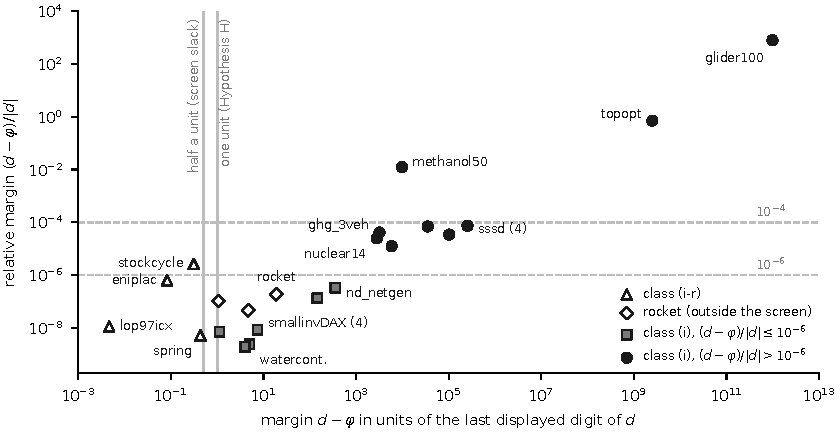
\includegraphics[width=\textwidth]{fig-audit-margins}
\caption{Margins $d-\varphi$ of the refuted listed dual bounds (class (i) and \inst{rocket}) and of the class (i-r) bounds, in units of the last displayed digit of $d=\dval{s}$ (horizontal) and relative to $|d|$ (vertical). $\varphi$ is the upper end of the objective enclosure at an exactly feasible point (for \inst{spring}, the proved optimum). Pairs with the same bound and point values are drawn once (19 class (i) pairs give 15 marks, 12 class (i-r) pairs give 4). Vertical lines: the slack of half a unit and the one unit of Hypothesis~H. Horizontal lines: MINLPLib's gap tolerance $10^{-6}$ and the common relative gap tolerance $10^{-4}$. Pages of 2026-09-30.}
\label{fig:audit-margins}
\end{figure}

\paragraph{Undecided pairs.}
Class (iii) mixes three situations.
For \inst{cecil_13}, \inst{hda}, \inst{heatexch_spec2} and the four \inst{rsyn} instances, the margin at the listed point is itself below half a display unit, so these pairs could at best become (i-r); the existence proofs failed on degenerate active sets or, for \inst{hda}, on a nonpolynomial active row over fixed variables.
For \inst{ex7_3_5}, \inst{ex8_2_1b}, \inst{sepasequ_complex} and \inst{sepasequ_convent}, Newton's method did not converge, the active set was degenerate, or one row could not be verified.
For \inst{oil} (\cref{sec:audit-limits}), the active equality system has 1,141 rows of rank 1,131 after all reductions, and its rows contain $\log_{10}$, $\ln$ and the power $0.8981$, so dependent rows can be removed only by a symbolic argument, which we did not attempt.
The listed violation of its point p2 is $4\cdot10^{-12}$ (our evaluation: $7.1\cdot10^{-11}$), and Gurobi lists the value of p2 as its own bound.

\paragraph{How MINLPLib aggregates.}
These are observations from the data, not documented rules.
The instance list shows a dual bound on 1,576 pages, exactly the pages with at least three per-solver entries when infeasibility claims (entries \texttt{inf}) count as entries.
Its 1,568 numeric values (the other eight are \texttt{inf}) equal, up to display rounding, the third-best per-solver entry with \texttt{inf} counted; with finite entries only, all but four match (\inst{ball_mk4_15}, \inst{chp_shorttermplan2c}, \inst{nuclear10a}, \inst{powerflow0057r}, each with one \texttt{inf} entry).
The 589 \texttt{=bestdual=} entries of \texttt{minlplib.solu} equal, for minimization, the smaller of the third-best entry and the lowest listed point value (for maximization, the larger of the third-best entry and the highest point value); 422 agree exactly and 167 within half a displayed unit.
This is consistent with the bold marking of the three best bounds \citep{vigerske2026-minlplib-documentation-database-snapshot-2026} and with the rule of \citet{vigerske2014-minlplib-2}.
We compared these aggregate values with the lower end of each proved objective enclosure, using one exactly feasible point per instance.
On the 15 class (i) instances and on \inst{rocket100}--\inst{rocket400}, the four \inst{emfl} instances, \inst{spring} and \inst{lop97icx}, neither the dual bound in the instance list nor the \texttt{=bestdual=} entry exceeds the lower end by more than display rounding.
On \inst{eniplac} and \inst{stockcycle}, the dual bound in the instance list is a six-digit (i-r) entry that exceeds a proved objective value by at least 0.083 and 0.31, which only the unproved rounding to six digits of \cref{app:audit-spring} explains; their \texttt{.solu} values are consistent with the proved points.
Otherwise the aggregate values agree with every proved point, and no solved mark is contradicted.

\begin{table}[t]
\centering\small
\caption{SHA-256 prefixes (12 hexadecimal digits) of the OSIL files used in \cref{sec:audit}, all identical to the live files at the refresh of 2026-10-02. Full hashes are in the archive.}
\label{tab:audit-inputs}
\begin{tabular}{@{}ll@{\qquad}ll@{}}
\toprule
instance & SHA-256 & instance & SHA-256 \\
\midrule
\inst{glider100} & \texttt{9eb2662396a8} & \inst{smallinvDAXr2b200-220} & \texttt{d401b1cdf468} \\
\inst{topopt-cantilever_60x40_50} & \texttt{64c5c8510630} & \inst{watercontamination0303} & \texttt{7fa81d273eea} \\
\inst{methanol50} & \texttt{7e64e24db3e0} & \inst{eniplac} & \texttt{95bcd431040f} \\
\inst{sssd20-04persp} & \texttt{b07166acea9a} & \inst{lop97icx} & \texttt{bdb9368cdb21} \\
\inst{sssd22-08persp} & \texttt{2912c22b8d99} & \inst{spring} & \texttt{9819238d7199} \\
\inst{sssd25-04persp} & \texttt{7954821c02c3} & \inst{stockcycle} & \texttt{ee74374e3d51} \\
\inst{sssd25-08persp} & \texttt{58fa3ae9a27b} & \inst{emfl050_3_3} & \texttt{697d84fb4974} \\
\inst{ghg_3veh} & \texttt{3831bb6b455d} & \inst{emfl050_5_5} & \texttt{501dd45c154f} \\
\inst{nuclear14} & \texttt{37644467e1df} & \inst{emfl100_3_3} & \texttt{730d7ee662cd} \\
\inst{nd_netgen-2000-3-4-b-a-ns_7} & \texttt{6f9b3bd97e56} & \inst{emfl100_5_5} & \texttt{eeddebe5ff1b} \\
\inst{smallinvDAXr1b150-165} & \texttt{593ae4de8591} & \inst{rocket100} & \texttt{fa26d3cbff49} \\
\inst{smallinvDAXr2b150-165} & \texttt{234295e83620} & \inst{rocket200} & \texttt{7b1892c4e946} \\
\inst{smallinvDAXr1b200-220} & \texttt{819f3a6a9f92} & \inst{rocket400} & \texttt{28b092a0fc0a} \\
\bottomrule
\end{tabular}
\end{table}

\subsection{The display hypothesis}\label{app:audit-hyp}

\begin{lemma}[when Hypothesis~H holds]\label{lem:audit-display}
Let $b\in\R$ be a reported dual bound and $s$ the string displayed for it, with $\dval{s}\neq0$.
\begin{enumerate}
\item[(a)] Suppose $\dval{s}$ arises from $b$ by finitely many steps, each a rounding (to nearest with any tie rule, or directed) or a truncation to an integer multiple of a power of ten.
Then $|b-\dval{s}|<\tfrac{10}{9}\dunit{s}$.
If at most one step changes the value, or if the last step that changes it rounds to nearest, Hypothesis~H holds.
\item[(b)] Suppose the site stores a binary64 number $b'$ with $|b'-b|\le 2^{-53}|b|$, rounds $b'$ to nearest at ten significant digits, stores the result in binary64, and displays it rounded to nearest at eight decimals without trailing zeros.
If $|\dval{s}|\le 6\cdot10^{7}$, Hypothesis~H holds.
\end{enumerate}
\end{lemma}

\begin{proof}
(a) Let $b_0=b$ and $b_k=R_k(b_{k-1})$ for $k=1,\dots,K$, where $R_k$ rounds or truncates to an integer multiple of a power of ten $w_k$, and $b_K=\dval{s}$.
Steps with $b_k=b_{k-1}$ can be dropped.
If none remains, $b=\dval{s}$ and Hypothesis~H holds because $\dunit{s}>0$.
Otherwise renumber the remaining steps $1,\dots,k$ with units $v_1,\dots,v_k$.
For $i\ge2$ the value $b_{i-1}$ is an integer multiple of $v_{i-1}$ but not of $v_i$, since otherwise step $i$ would not change it; as both units are powers of ten, $v_i>v_{i-1}$, and hence $v_i\le10^{i-k}v_k$.
A rounding or truncation to multiples of $v$ moves a number by less than $v$, and rounding to nearest by at most $v/2$.
Hence
\[
  |b-\dval{s}|\le\sum_{i=1}^{k}|b_i-b_{i-1}|<\sum_{i=1}^{k}v_i\le v_k\sum_{m\ge0}10^{-m}=\tfrac{10}{9}v_k .
\]
Since $\dval{s}=b_k$ is a nonzero integer multiple of $v_k$, $\dunit{s}\ge v_k$, which proves the first claim.
If $k=1$, then $|b-\dval{s}|<v_1\le\dunit{s}$.
If the last step rounds to nearest, then $|b-\dval{s}|<\tfrac12v_k+\sum_{i<k}v_i\le(\tfrac12+\tfrac19)v_k<\dunit{s}$.

(b) Since $\dval{s}\ne0$, also $b'\ne0$.
Let $e=\lfloor\log_{10}|b'|\rfloor$ and $v_1=10^{e-9}$, the unit of the tenth significant digit of $b'$; then $v_1>10^{-10}|b'|$.
Let $r$ be $b'$ rounded to nearest at $v_1$, let $r'=\fl(r)$, let $v_2=10^{-8}$, and let $\dval{s}$ be $r'$ rounded to nearest at $v_2$.
Then $|b'-r|\le v_1/2$, $|r-r'|\le2^{-53}|r|$ and $|r'-\dval{s}|\le v_2/2$.

\emph{Case $v_1\ge v_2$.}
Then $r$ is an integer multiple of $v_2$.
From $|r'|\le|\dval{s}|+v_2/2<2^{26}$ and the monotonicity of rounding, $|r|<2^{26}$, so the spacing of binary64 numbers near $r$ is at most $2^{-27}$ and $|r-r'|\le2^{-28}<v_2/2$.
The multiple of $v_2$ nearest to $r'$ is therefore $r$, so $\dval{s}=r$.
This is a nonzero integer multiple of $v_1$, hence $\dunit{s}\ge v_1$.
Finally $|b-\dval{s}|\le|b-b'|+|b'-r|\le2^{-53}|b|+v_1/2<v_1$, because $2^{-52}|b|\le2^{-52}|b'|/(1-2^{-53})<10^{-10}|b'|<v_1$.

\emph{Case $v_1<v_2$.}
Then $v_1\le v_2/10$, $e\le0$, $|b'|<10$, $|r|\le10$ and $|b|<10.1$.
Summing the four errors,
\[
  |b-\dval{s}|\le2^{-53}(|b|+|r|)+\tfrac{1}{20}v_2+\tfrac12v_2<v_2\le\dunit{s},
\]
where the last inequality holds because $\dval{s}$ is a nonzero integer multiple of $v_2$.
\end{proof}

The pages are consistent with rule (b): of the 13,847 finite values they display, 13,723 are fixed points of the rule ``round to ten significant digits, print at eight decimals, remove trailing zeros'', 122 others differ only in the sign of zero, and two show more digits than the rule allows.
The rule cannot be verified from the pages alone, which is why the refutations rest on the weaker Hypothesis~H.

\begin{remark}[why (b) needs a size condition]\label{rem:audit-fac1}
The page of \inst{fac1} shows $160912612.40000001$, the eight-decimal print of the binary64 number nearest to $160912612.4$.
For this string $\dunit{s}=10^{-8}$, while a reported number that rounds to $160912612.4$ at ten significant digits may differ from $\dval{s}$ by up to $0.05$; the condition $|\dval{s}|\le6\cdot10^{7}<2^{26}$ excludes such strings.
\end{remark}

\subsection{Existence certificates}\label{app:audit-existence}

\paragraph{The Krawczyk test in midpoint–radius form.}
Both implementations evaluate the following form of \cref{thm:pts-krawczyk}, whose hypotheses they check exactly.
Absolute values and inequalities of vectors and matrices are entrywise.

\begin{lemma}[midpoint–radius Krawczyk test]\label{lem:audit-krawczyk}
Let $G:\R^n\to\R^n$ be continuously differentiable on an open set containing the box $X=\{x:|x-\tilde x|\le r\}$ with $r>0$.
Suppose $|G(\tilde x)-G_c|\le G_r$, and for every $\xi\in X$ and every row $i$, $|\nabla G_i(\xi)^{\mathsf T}-(J_c)_{i,:}|\le(J_r)_{i,:}$.
Let $R\in\R^{n\times n}$ and
\[
  \beta:=|RG_c|+|R|G_r+|I-RJ_c|\,r+|R|\,J_r\,r .
\]
If $\beta<r$, then $G$ has exactly one zero in $X$.
\end{lemma}

\begin{proof}
Apply the first part of \cref{thm:pts-krawczyk}, whose proof (\cref{app:points-krawczyk}) uses only that $G$ is continuously differentiable on an open set containing $X$, with $y=\tilde x$, $C=R$, $\mathbf v=[G_c-G_r,G_c+G_r]$, $\mathbf A=[J_c-J_r,J_c+J_r]$ and $\mathbf B=[I-RJ_c-|R|J_r,\,I-RJ_c+|R|J_r]$.
Then $G(\tilde x)\in\mathbf v$, $G'(\xi)\in\mathbf A$ on $X$, and $I-RA\in\mathbf B$ for every $A\in\mathbf A$, since $|(I-RA)-(I-RJ_c)|\le|R|J_r$.
For $v\in\mathbf v$, $M\in\mathbf B$ and $x\in X$, $|\tilde x-Rv+M(x-\tilde x)-\tilde x|\le|RG_c|+|R|G_r+(|I-RJ_c|+|R|J_r)\,r=\beta$, so $K=[\tilde x-\beta,\tilde x+\beta]$ satisfies (c), and $K\subseteq\operatorname{int}X$ because $\beta<r$.
\end{proof}

\begin{corollary}[exactly feasible point]\label{cor:audit-box}
In a Krawczyk proof (\cref{sec:audit-existence}), let $E$ be the active rows, $x_N$ the fixed values of the nonbasic variables, and $G(x_B)=g_E(x_B,x_N)-t_E$, where $t_E$ holds each active row at its side.
Suppose \cref{lem:audit-krawczyk} applies on a box $X$ of basic values, every expression of the model is defined on $X\times\{x_N\}$, and
(i) every row outside $E$ satisfies its bounds on all of $X\times\{x_N\}$, where an equality row passes only if it is constant there and equal to its side;
(ii) $X$ lies within the bounds of the basic variables;
(iii) $x_N$ satisfies its bounds and integrality requirements exactly, and every integer variable is nonbasic.
Then the zero $x_B^\ast$ yields $x^\ast=(x_B^\ast,x_N)\in\feas$, and $f(x^\ast)$ lies in every enclosure of $f$ over $X\times\{x_N\}$.
\end{corollary}

\begin{proof}
$G(x_B^\ast)=0$ puts every active row at its side, (i) covers the other rows, and (ii) and (iii) cover bounds and integrality.
\end{proof}

The implementations accept an equality row outside $E$ only if it vanishes identically as a polynomial in the basic variables or its interval enclosure is a single point equal to its side; an enclosure of positive width never passes, so no equality is accepted by accident.
Enclosures of a division or a square root whose argument interval touches 0 abort the proof.
The class (i) and \inst{rocket} files use only sums, products, negation, division, squares, integer powers, $\exp$ and $\sqrt{\cdot}$.

\paragraph{Floating-point error terms.}
Both implementations compute $R$ as an approximate inverse in binary64 and evaluate the products in $\beta$ in binary64.
Let $\uround=2^{-53}$, $\eta=2^{-1074}$ and $\gamma_m=m\uround/(1-m\uround)$.

\begin{lemma}[rounding errors of matrix products]\label{lem:audit-fp}
Let $A\in\mathbb F^{n\times m}$ and $B\in\mathbb F^{m\times p}$ be binary64 matrices with $m\uround<\tfrac12$, and let $\widehat C$ be their product computed in binary64 with round to nearest, in any order of summation, with or without fused multiply–add, and without overflow.
Then $|\widehat C-AB|\le\gamma_m|A|\,|B|+m\eta$ entrywise.
\end{lemma}

\begin{proof}
Fix an entry $c=\sum_{i=1}^m a_ib_i$.
Each rounding of a product or of a fused multiply–add returns $z(1+\varepsilon)+\delta$ with $|\varepsilon|\le\uround$ and $|\delta|\le\eta/2$, and each rounding of a sum returns $z(1+\varepsilon)$, because sums are exact in the underflow range \citep[Section~2]{rump2010-verification-methods-rigorous-results-using}.
Following each term through the computation, $\hat c=\sum_i a_ib_i\theta_i+\sum_j\delta_j\theta'_j$, where each $\theta_i$ is a product of at most $m$ factors $1+\varepsilon$, each $\theta'_j$ of at most $m-1$ such factors, and there are at most $m$ terms $\delta_j$.
Hence $|\theta_i-1|\le\gamma_m$ and $|\theta'_j|\le1+\gamma_{m-1}\le2$, which gives the bound.
Without underflow this is the classical bound; see Theorem~2.1 of \citet{rump2010-verification-methods-rigorous-results-using}.
\end{proof}

The audit implementation computes $G(\tilde x)$ and the Jacobian over $X$ by forward-mode automatic differentiation in mpmath interval arithmetic at 40 digits, starting from the exact decimals, and converts the results outward to binary64 midpoint–radius pairs.
It bounds each product in $\beta$ by \cref{lem:audit-fp}, multiplies by $(1+10^{-6})^2$ to cover the roundings of the bound computations themselves (whose relative size is below $n\uround\approx4.4\cdot10^{-13}$ for $n\le4000$), and adds $10^{-300}$ per entry for underflow.
It encloses $F$ and the Jacobian over a box whose binary64 endpoints are moved outward by one unit in the last place, and it uses as $r_i$ the smaller distance from $\tilde x_i$ to the two endpoints, so the hypotheses of \cref{lem:audit-krawczyk} hold on a box inside the enclosed one.
The separately written implementation (checker V1 below) computes the same quantities in its own interval arithmetic with rational endpoints rounded outward to 200 bits: $+,-,\times,\div$ and integer powers are exact before rounding, square roots use integer square roots, and $\exp$ and $\log$ use mpmath at 90 digits, widened by a relative $10^{-60}$.
It bounds the binary64 products by \cref{lem:audit-fp} with a factor 2 on the error terms and explicit underflow terms $k\eta$, and multiplies the result by $1+10^{-12}$; its box has exact rational endpoints.
Inspection of the code confirmed both bound computations.

\paragraph{The proof methods in detail.}
The Krawczyk proof rounds and fixes the integer variables and puts continuous variables within $10^{-7}$ (relative) of a bound on it.
The active rows are all equality rows and the inequality rows that are violated or within $10^{-7}$ of a side, held at that side; rows with vanishing gradient in the free variables move to the box check.
A basis of $|E|$ continuous variables is chosen by QR factorization with column pivoting, favouring variables away from their bounds, and the other variables keep their exact decimals.
Newton's method (residuals at 40 digits) gives the centre of a box of relative radius $10^{-12}$, $10^{-10}$ or $10^{-8}$ for the Krawczyk test, and the box check of \cref{cor:audit-box} encloses every other row, exactly in the basic variables where the row is polynomial and by intervals otherwise, and the objective.
A basic variable that ends on a bound is fixed there and the attempt repeated.
The shifted Krawczyk proof first fixes, repeatedly, every continuous variable that a linear row determines alone; two linear programs (HiGHS) then give a direction that keeps the linearized equalities, strictly improves as many active inequalities and bounds as possible and changes the objective least, and a Krawczyk proof follows at a point moved along it by a distance $t$ that grows by factors of ten from three times the violation.
The linear programs only propose the point; the Krawczyk proof proves it.

The dedicated proofs end with an exact check of every row and bound of the OSIL model, except the one for \inst{topopt-cantilever_60x40_50}, which ends with the box check of the Krawczyk proof.
For \inst{watercontamination0303}, all rows are linear and the objective is quadratic; the 14 binaries are rounded, the 1,008 bounded source variables keep their decimals, and the other 106,200 variables follow exactly from equality rows with a single unknown (largest change $1.6\cdot10^{-13}$).
For \inst{nd_netgen-2000-3-4-b-a-ns_7}, the binaries are kept; the 74 flow-conservation rows are made to hold exactly by rational Gauss--Jordan elimination on flows strictly inside their bounds (largest change $2.1\cdot10^{-13}$; the two dependent rows hold exactly), then $u:=\max(u,cf^2)$ on each arc, and $s,t$ follow from their defining rows, so each rotated cone row $cf^2+s^2-t^2\le0$ holds.
For \inst{topopt-cantilever_60x40_50}, the binaries are kept and the stresses of void elements are exactly 0 in the listed points and stay 0, so their cone rows read $0\le0$; the 3,162 (p5) or 3,056 (p4) equality rows that involve the stresses of the 1,200 solid elements are linear, and a linear Krawczyk test on a QR basis of these stresses proves a unique solution in a box (largest ratio $\beta_i/r_i$ about 0.011 at relative radius $10^{-14}$); each cost variable $c_e$ is then set to the upper end of an interval enclosure of $\sum_k w_{e,k}^2$ over the box, so every solid cone row holds and the objective $\sum_ec_e$ is an exact rational.

\paragraph{The \inst{glider100} point.}
Point p2 of \inst{glider100}, an ``other point'' with listed violation $3\cdot10^{-8}$ (exact evaluation: $1.2\cdot10^{-7}$), has objective value about $-983842.26$.
The shifted Krawczyk proof moves it by $1.75\cdot10^{-10}$ (\cref{tab:audit-second}); V1 proves a nearby point with the altitude at node 1 fixed at its bound 0.
Both describe the same trajectory: 100 steps of about 621.6\,s, an altitude that drops to 0 at node 1, rises to about 64.6\,km and ends at 900\,m, and a vertical acceleration that changes sign at every node, so that the trapezoidal averages nearly cancel.
This period-2 mode of the discretization is feasible for the model as stored; its range of about 983.8\,km compares with 1.26\,km at the listed point p1.

\paragraph{Second implementations.}
Two checkers, written separately from the audit code and from each other in separate agent sessions, re-proved the 19 class (i) pairs.
Checker V1 has its own OSIL reader with exact fractions, the interval arithmetic and Krawczyk test described above, and its own exact certificates; it covered 14 pairs and re-fetched the OSIL files and points, which were byte-identical to ours.
Checker V2 has its own reader and uses exact rational constructions only; it covered the other five pairs and recomputed every count, margin and class from the data files.
Every second proof gives an exactly feasible point whose objective value is at most the audit's upper end $\varphi$ (\cref{tab:audit-second}; for \inst{watercontamination0303} the two exact values agree in all 16 digits shown), so every margin of \cref{tab:audit-pairs} holds under either implementation.

\begin{table}[t]
\centering\footnotesize
\setlength{\tabcolsep}{3pt}
\caption{Existence proofs of the 15 class (i) conflicts. $n$: size of the square system; ratio: largest $\beta_i/r_i$ of \cref{lem:audit-krawczyk} in the audit implementation. Audit proof: method of \cref{sec:audit-existence}. Second proof: checker and method. Last column: upper end of the objective enclosure of the second proof's exactly feasible point, rounded up, or its exact value truncated as marked by ``\dots''.}
\label{tab:audit-second}
\begin{tabular}{@{}>{\raggedright\arraybackslash}p{0.3\textwidth}>{\raggedright\arraybackslash}p{0.22\textwidth}>{\raggedright\arraybackslash}p{0.2\textwidth}l@{}}
\toprule
instance (point) & audit proof & second proof & second $\varphi$ \\
\midrule
\inst{glider100} (p2) & shifted Krawczyk, $n=1208$, ratio $1.0\cdot10^{-4}$ & V1, Krawczyk, $n=1209$ & $-983842.2577881223$ \\
\inst{topopt-cantilever_60x40_50} (p5) & dedicated, linear Krawczyk, ratio $0.011$ & V1, exact Gram system and Krawczyk & $10.33547427574701$ \\
\inst{methanol50} (p4) & Krawczyk, $n=1497$, ratio $2\cdot10^{-3}$ & V1, Krawczyk & $0.0079302187993$ \\
\inst{sssd20-04persp} (p3) & Krawczyk, $n\le16$ & V1, Krawczyk; V2, exact & $347691.41048398308\dots$ \\
\inst{sssd22-08persp} (p4) & Krawczyk, $n\le16$ & V2, exact & $508713.73101118680506\dots$ \\
\inst{sssd25-04persp} (p3) & Krawczyk, $n\le16$ & V2, exact & $300176.56366586825118\dots$ \\
\inst{sssd25-08persp} (p4) & Krawczyk, $n\le16$ & V2, exact & $472093.07796988413312\dots$ \\
\inst{ghg_3veh} (p2) & Krawczyk, $n=52$, ratio $7.3\cdot10^{-5}$ & V1, Krawczyk & $7.754006050057346$ \\
\inst{nuclear14} (p3) & Krawczyk, $n=434$ & V1, Krawczyk & $-1.12968744117115$ \\
\inst{nd_netgen-2000-3-4-b-a-ns_7} (p2) & dedicated, exact & V1, exact (least $u$) & $10729657.585117233\dots$ \\
\inst{smallinvDAXr1b150-165}, \inst{smallinvDAXr2b150-165} (p2) & listed-point check & V1, V2, exact & $88.10493476$ \\
\inst{smallinvDAXr1b200-220}, \inst{smallinvDAXr2b200-220} (p2) & Krawczyk, $n=1$ & V1, V2, exact & $156.604267884$ \\
\inst{watercontamination0303} (p2) & dedicated, exact & V1, exact & $207.9850348023888\dots$ \\
\bottomrule
\end{tabular}
\end{table}

\begin{certbox}[Certificate for the class (i) refutations (\cref{tab:audit-pairs})]
\certitem{Inputs}{OSIL files of the 15 instances (SHA-256 prefixes in \cref{tab:audit-inputs}); MINLPLib's \texttt{.sol} files of the listed points; the pages of 2026-09-30.}
\certitem{Computation}{listed-point checks and the dedicated proofs for \inst{watercontamination0303} and \inst{nd_netgen-2000-3-4-b-a-ns_7}: rational arithmetic \arith{E}; Krawczyk proofs, shifted or not, and the \inst{topopt-cantilever_60x40_50} certificate: interval Jacobians in mpmath \arith{I}, Krawczyk inequality in binary64 with a priori error terms \arith{F} (\cref{lem:audit-fp}).}
\certitem{Data reading}{exact decimals or outward enclosures of them, in both implementations (confirmed by inspection of the code).}
\certitem{Implementations}{the audit implementation certifies the values $\varphi$ of \cref{tab:audit-pairs}; the second proves an exactly feasible point with objective value at most $\varphi$ for every pair (\cref{tab:audit-second}).}
\certitem{Evidence level}{\evid{hand} (\cref{prop:audit-refute}) + \evid{stored}; for \inst{topopt-cantilever_60x40_50}, \evid{hand} + \evid{rerun}: its basis is not stored, so the point is regenerated, not replayed.}
\certitem{Replay}{Tier~1; seconds per point; about 3\,min per \inst{topopt-cantilever_60x40_50} point.}
\end{certbox}

\paragraph{Trust and replay.}
Of the seven Krawczyk-based refutations (\cref{sec:audit-existence}), \inst{methanol50}, \inst{nuclear14} and \inst{topopt-cantilever_60x40_50} have rational enclosures in V1, with no transcendental function; for \inst{glider100} and \inst{ghg_3veh}, the audit needs correct outward rounding of mpmath's interval $\exp$ and $\sqrt{\cdot}$, and V1 needs mpmath's $\exp$ at 90 digits to be accurate far beyond its widening of $10^{-60}$.
Negative controls behaved as expected: moving a Krawczyk centre for \inst{methanol50} by $10^{-11}$ (relative) makes the test fail at radius $10^{-12}$ and pass at radius $10^{-11}$; tightening an inactive row of \inst{ghg_3veh} by $10^{-9}$ below its value makes the box check fail at that row; and the listed-point check rejects a point once a bound cuts off one of its values.
The \inst{topopt-cantilever_60x40_50} certificate does not store its basis, and its centre file prints values at 25 to 45 digits, so it is regenerated rather than replayed (\cref{app:repro-regen}).
With one BLAS thread, pivoted QR chooses another basis, and the regeneration proves another exactly feasible point, with objective value $10.33547432783171797\ldots$; V1's point has objective value at most $10.33547427574701$.
Both lie below the displayed $\varphi\le10.33547433$ of the archived point, so the row of \cref{tab:audit-pairs} holds for all three points.

\subsection{The class (i-r) pairs and the \texorpdfstring{\inst{spring}}{spring} optimum}\label{app:audit-spring}

The OSIL model of \inst{spring} (identical to its GAMS form) has the variables $x_1\ge0.414$, $x_2\ge0.207$, $x_3\in[\lambda,0.02]$, an integer $i_4\in[1,100]$, $x_5\ge1.1$, a free $x_6$ and binaries $b_7,\dots,b_{17}$.
Its rows are
\begin{gather*}
  x_5=x_1/x_2,\qquad x_6=\frac{4x_5-1}{4x_5-4}+\frac{0.615}{x_5},\qquad \frac{2546.47908913782\,x_6x_5}{x_2^2}\le189000,\\
  x_3=\frac{K\,x_5^3\,i_4}{x_2},\qquad 2.1x_2+1000x_3+1.05\,x_2i_4\le14,\qquad x_1+x_2\le3,\\
  x_2=\sum_{k=7}^{17}c_kb_k,\qquad \sum_{k=7}^{17}b_k=1,
\end{gather*}
with $(c_7,\dots,c_{17})=(0.207,0.225,0.244,0.263,0.283,0.307,0.331,0.362,0.394,0.4375,0.5)$, and the objective is $(a_0+a_1i_4)\,x_1x_2^2$.

\begin{proposition}[\inst{spring}]\label{prop:spring-opt}
With $a_0=1.570796327$, $a_1=0.7853981635$, $c=0.283$, $\lambda=1.78571428571429\cdot10^{-3}$, $K=6.95652173913044\cdot10^{-7}$ and $x_5^\ast=\bigl(\lambda c/(9K)\bigr)^{1/3}$, the optimal value of \inst{spring} is $\vstar=(a_0+9a_1)\,c^{3}\,x_5^\ast=0.846245665643154281251664635037\ldots$, attained with $i_4=9$, $x_2=0.283$ and $x_3=\lambda$.
The five displayed bounds 0.84624567 equal $\vstar$ rounded to eight decimals.
\end{proposition}

\begin{proof}
The last two rows and integrality give $x_2=c$ for exactly one $c\in\{c_7,\dots,c_{17}\}$.
Fix $i_4=n$ and $x_2=c$.
The equality rows then determine $x_1=cx_5$, $x_3=Knx_5^3/c$ and $x_6$ as functions of $x_5$, and the objective becomes $(a_0+a_1n)c^3x_5$, which is increasing in $x_5$.
Each remaining condition is a closed interval in $x_5$: the bounds give $x_5\ge1.1$ and $x_5\ge0.414/c$; the bounds on $x_3$ give $(\lambda c/(Kn))^{1/3}\le x_5\le(0.02c/(Kn))^{1/3}$; the fifth row gives $x_5^3\le(14-2.1c-1.05cn)\,c/(1000Kn)$; and the sixth gives $x_5\le(3-c)/c$.
For the third row, $x_6x_5=h(x_5)+0.615$ with
\[
  h(x)=\frac{x(4x-1)}{4(x-1)}=(x-1)+\frac74+\frac{3}{4(x-1)},\qquad h''(x)=\frac{3}{2(x-1)^3}>0\quad(x>1),
\]
so the row reads $h(x_5)\le189000c^2/2546.47908913782-0.615$, and the sublevel set of the convex function $h$ is an interval.
Hence the feasible values of $x_5$ for $(n,c)$ form a closed interval $I(n,c)$, possibly empty, and
\[
  \vstar=\min_{n,c}\,(a_0+a_1n)\,c^3\min I(n,c),
\]
the minimum over the nonempty intervals.

At $(n,c)=(9,0.283)$ the condition $x_3\ge\lambda$ gives $x_5\ge x_5^\ast=(\lambda c/(9K))^{1/3}\approx4.3217$, which exceeds the other lower bounds $1.1$ and $0.414/0.283\approx1.463$.
At $x_5^\ast$ every other condition holds: the third row evaluates to about $187991.19\le189000$, the fifth to about $5.054\le14$, the sixth to about $1.506\le3$, and $x_3=\lambda\le0.02$.
So $x_5^\ast\in I(9,0.283)$ and every element of $I(9,0.283)$ is at least $x_5^\ast$; hence $\min I(9,0.283)=x_5^\ast$, with value $(a_0+9a_1)\,0.283^3\,x_5^\ast$, attained by $i_4=9$, $b_{11}=1$, $x_5=x_5^\ast$ and the other variables defined by the equality rows.

The comparison with the other $1{,}099$ assignments is computer-assisted and exact.
One program enumerates all 1,100 assignments, brackets every cube root between rationals checked by exact cubing, and finds 890 assignments infeasible and 210 feasible, with every other minimum above the value at $(9,0.283)$; the second smallest is $0.8592755352970280\ldots$, at $(5,0.307)$.
A separately written program excludes 723 assignments by the bounds on $x_3$ and the fifth and sixth rows, and shows with exact comparisons (and rational brackets of cube roots and of $\sqrt3$) that no assignment reaches an objective value at or below a rational $T$ slightly below the value at $(9,0.283)$.
Together with an exactly feasible point, this gives, without the first program,
\begin{multline*}
  \vstar\in[0.84624566564315428125166463503714129527532857794010,\\
  0.84624566564315428125166463503714129527534815925597].
\end{multline*}
This enclosure rounds to 0.84624567 at eight decimals.
\end{proof}

\begin{certbox}[Certificate for \cref{prop:spring-opt}]
\certitem{Inputs}{\inst{spring} OSIL file (SHA-256 \texttt{9819238d7199}\dots).}
\certitem{Computation}{reduction to one variable per assignment (a written argument, checked exactly against the model at 200 random rational points); exact enumeration of the 1,100 assignments with cube roots bracketed by rationals \arith{E}.}
\certitem{Data reading}{exact decimals.}
\certitem{Implementations}{two separately written exact programs, one enumerating all minima and one excluding assignments by bounds; a 60-digit scan reproduces the 210 feasible assignments and the three smallest minima (evidence only).}
\certitem{Evidence level}{\evid{hand} + \evid{stored}.}
\certitem{Replay}{Tier~1; seconds.}
\end{certbox}

The best listed primal value of \inst{spring}, 0.8462441, lies more than $1.5\cdot10^{-6}$ below $\vstar$.

\paragraph{The other class (i-r) pairs.}
\Cref{tab:audit-ir} lists all 12 pairs.
For \inst{lop97icx} and \inst{stockcycle} the listed point is exactly feasible as listed.
For \inst{eniplac}, the listed point violates 31 equality rows by $4.8\cdot10^{-14}$ to $2.5\cdot10^{-10}$; an exactly feasible point keeps 36 listed decimals and the binaries and recomputes the other 81 variables from equality rows that are linear in them.
All these proofs are in exact rational arithmetic, by a checker written separately from the audit code, and agree with the audit's enclosures.
The last column of \cref{tab:audit-ir} shows that the page's own display rule (\cref{lem:audit-display}(b)) cannot explain the conflicts on \inst{eniplac}, \inst{lop97icx} and \inst{stockcycle}: a stored value at or below the proved objective would display with more digits.
Rounding to six significant digits before storage would explain them: all seven displayed values equal the best listed point value of their instance rounded half up to six significant digits, and the same pages show other bounds with nine or ten digits (for example BARON's $-132117.083$ on \inst{eniplac}).
Among the bounds dated 2013-09-17, 59 show exactly six significant digits and only 2 show seven, while among all other bounds seven-digit values are more common than six-digit ones (471 against 263).
This supports the explanation but does not prove it.

\begin{table}[t]
\centering\footnotesize
\setlength{\tabcolsep}{3pt}
\caption{The 12 class (i-r) pairs, all dated 2013-09-17. Solvers: \inst{eniplac} COUENNE, LINDO and SCIP; \inst{lop97icx} ANTIGONE; \inst{spring} ANTIGONE, BARON, COUENNE, LINDO and SCIP; \inst{stockcycle} ANTIGONE, BARON and COUENNE. $\varphi$: objective value of an exactly feasible point (exact; ``\dots'' marks truncation). Slack: half a unit in the last displayed digit. Last column: $d-\varphi$ divided by half a unit in the tenth significant digit or the eighth decimal, whichever is coarser.}
\label{tab:audit-ir}
\begin{tabular}{@{}llllll@{}}
\toprule
instance & $d$ & $\varphi$ & $d-\varphi$ & $(d-\varphi)/\text{slack}$ & $(d-\varphi)/\text{page half-unit}$ \\
\midrule
\inst{eniplac} & $-132117.$ & $-132117.0830199887\dots$ & $0.08301\dots$ & $0.166\dots$ & $1660\dots$ \\
\inst{lop97icx} & $4099.06$ & $4099.059953600000099$ & $4.6399999901\cdot10^{-5}$ & $0.00927\dots$ & $92.7\dots$ \\
\inst{spring} & $0.84624567$ & $0.8462456656431542\dots$ & $4.3568\dots\cdot10^{-9}$ & $0.871\dots$ & $0.871\dots$ \\
\inst{stockcycle} & $119949.$ & $71969213/600$ & $187/600$ & $0.623\dots$ & $6233\dots$ \\
\bottomrule
\end{tabular}
\end{table}

\subsection{The \texorpdfstring{\inst{emfl}}{emfl} instances}\label{app:audit-emfl}

The certificate code checks, from each OSIL file, that the instance has the form
\begin{equation}\label{eq:audit-emfl}
  \min\ \sum_{k}c_kt_k\quad\text{s.t.}\quad t_k^2-\|w_k\|^2\ge0,\ t_k\ge0,\quad w_k=A_kz+e_k,\quad z_j\ge0\ (j\in P),\ z_j\ \text{free}\ (j\notin P),
\end{equation}
with rational data and $c_k\ge0$, where each component of each $w_k$ is a variable defined by one linear equality row, and that there are no other rows, no objective constant and no integer variables.
The four instances have 531, 1,875, 981 and 3,125 cones and 18, 50, 18 and 50 base variables $z$.

\begin{lemma}[weak duality for \eqref{eq:audit-emfl}]\label{lem:audit-socp}
\begin{enumerate}
\item[(a)] If a rational $\bar z$ satisfies the sign constraints and rationals $\tau_k\ge0$ satisfy $\tau_k^2\ge\|A_k\bar z+e_k\|^2$, then $(\bar z,(A_k\bar z+e_k)_k,\tau)$ is exactly feasible and $\vstar\le\sum_kc_k\tau_k$.
\item[(b)] If rational vectors $y_k$ satisfy $\|y_k\|^2\le c_k^2$, and $g:=\sum_kA_k^{\mathsf T}y_k$ satisfies $g_j\ge0$ for $j\in P$ and $g_j=0$ for $j\notin P$, then $\vstar\ge\sum_ke_k^{\mathsf T}y_k$.
\end{enumerate}
\end{lemma}

\begin{proof}
(a) holds by construction.
For (b), let $(z,w,t)$ be feasible.
From $t_k\ge0$ and $t_k^2\ge\|w_k\|^2$ we get $t_k\ge\|w_k\|$, and by the Cauchy--Schwarz inequality $c_kt_k\ge c_k\|w_k\|\ge\|y_k\|\,\|w_k\|\ge y_k^{\mathsf T}w_k$.
Summing, $\sum_kc_kt_k\ge\sum_ky_k^{\mathsf T}(A_kz+e_k)=g^{\mathsf T}z+\sum_ke_k^{\mathsf T}y_k\ge\sum_ke_k^{\mathsf T}y_k$, since $g_jz_j\ge0$ for every $j$.
\end{proof}

\begin{proposition}[\inst{emfl}]\label{prop:emfl-enclosure}
For \inst{emfl050_3_3}, \inst{emfl050_5_5}, \inst{emfl100_3_3} and \inst{emfl100_5_5}, the optimal values lie in the first-line intervals of \cref{tab:audit-emfl}, each of width below $3.4\cdot10^{-11}$.
Every listed dual bound of these instances is valid.
The best listed primal values lie below $\vstar$ by at least $1.41\cdot10^{-5}$, $1.98\cdot10^{-3}$, $2.92\cdot10^{-4}$ and $6.86\cdot10^{-6}$, so no exactly feasible point attains them; for \inst{emfl050_3_3}, which is marked solved, this is at least $1.36\cdot10^{-6}$ relative.
\end{proposition}

\begin{proof}
Apply \cref{lem:audit-socp}.
The points $\bar z$ are rational roundings of a numerical solution of the cone program; $w$ is computed exactly, and $\tau_k$ is a rational upper bound of $\|w_k\|$ obtained from an integer square root.
The vectors $y_k$ start from a numerical dual solution and are made exactly admissible: checker V2 scales each cone to a radius slightly below $c_k$, corrects negative $g_j$ by moves within single cones and applies a final scaling; the audit makes $g=0$ exactly by a rational least-norm correction and then scales all $y_k$ by one rational factor.
Both conditions of (b) and both objective values are evaluated in rational arithmetic.
This gives the enclosures of \cref{tab:audit-emfl}.
Every listed dual bound is at most the lower end, so it is valid.
The best listed primal value plus half a unit in its last displayed digit is below the lower end by the stated amounts, so no exactly feasible point attains it.
\end{proof}

\begin{table}[t]
\centering\footnotesize
\setlength{\tabcolsep}{3pt}
\caption{Enclosures of the optimal values of the \inst{emfl} instances (outward displays; first line: checker V2, second line: audit implementation). Best listed dual and best listed primal value (point, listed violation) from the pages of 2026-09-30. Shortfall: lower end minus the best listed primal value widened by half a display unit, rounded down. $^{\checkmark}$: marked solved on MINLPLib.}
\label{tab:audit-emfl}
\begin{tabular}{@{}ll>{\raggedright\arraybackslash}p{0.16\textwidth}>{\raggedright\arraybackslash}p{0.355\textwidth}l@{}}
\toprule
instance & best listed dual & best listed primal & $\vstar\in$ & shortfall $\ge$ \\
\midrule
\inst{emfl050_3_3}$^{\checkmark}$ & $10.40173999$ & $10.40173793$ (p2, $2\cdot10^{-10}$) & $[10.4017521318429,\,10.4017521318448]$ \newline $[10.4017521316,\,10.4017521319]$ & $1.41\cdot10^{-5}$ \\
\inst{emfl050_5_5} & $18.91340776$ & $18.91165289$ (p6, $10^{-8}$) & $[18.9136329557291,\,18.9136329557624]$ \newline $[18.9136329529,\,18.9136329563]$ & $1.98\cdot10^{-3}$ \\
\inst{emfl100_3_3} & $18.13262446$ & $18.13236088$ (p4, $10^{-8}$) & $[18.1326531242336,\,18.1326531242359]$ \newline $[18.1326531194,\,18.1326531244]$ & $2.92\cdot10^{-4}$ \\
\inst{emfl100_5_5}$^{\checkmark}$ & $32.63818348$ & $32.63818348$ (p1, $10^{-10}$) & $[32.6381903545115,\,32.6381903545301]$ \newline $[32.6381903513,\,32.6381903548]$ & $6.86\cdot10^{-6}$ \\
\bottomrule
\end{tabular}
\end{table}

All listed points of the four instances except p3 of \inst{emfl050_3_3} lie below the exact optimum, the farthest by about $8.1\cdot10^{-3}$ (about $4.3\cdot10^{-4}$ relative; an ``other'' point of \inst{emfl050_5_5}); points with listed violations of $4\cdot10^{-11}$ to $8\cdot10^{-10}$ are among them, so even very small violations at the apex of a cone lower the objective visibly.
Checker V1, a third implementation, encloses the optimum of \inst{emfl050_3_3} in $[10.40175213184103,\,10.40175213184476]$.
The best listed dual bound of this instance, 10.40173999, lies at least $1.213\cdot10^{-5}$ (at least $1.166\cdot10^{-6}$ relative) below the exact optimum; its solved mark is consistent with the listed primal value 10.40173793, and since the mark is defined with tolerance-feasible points, we do not call it wrong.

\begin{certbox}[Certificate for \cref{prop:emfl-enclosure}]
\certitem{Inputs}{OSIL files of the four \inst{emfl} instances (SHA-256 prefixes in \cref{tab:audit-inputs}).}
\certitem{Computation}{rational primal points and rational dual vectors checked in exact arithmetic, square roots by integer square root \arith{E}; the numerical cone solver only proposes candidates.}
\certitem{Data reading}{exact decimals.}
\certitem{Implementations}{two for all four instances (the audit implementation and checker V2), a third (checker V1) for \inst{emfl050_3_3}; the displayed enclosures, and hence their widths, rest on checker V2 alone; the wider enclosures of the audit implementation (and of checker V1) also prove the validity of every listed dual bound and the stated shortfalls, so these verdicts are verified by a separately written implementation.}
\certitem{Evidence level}{\evid{hand} (\cref{lem:audit-socp}) + \evid{rerun}: the rational dual vectors are not stored; a rerun solves the cone programs again and checks the new vectors exactly, and may give slightly different, equally valid endpoints.}
\certitem{Replay}{Tier~1; seconds to minutes per instance.}
\end{certbox}

\subsection{The \texorpdfstring{\inst{rocket}}{rocket} instances}\label{app:audit-rocket}

The \inst{rocket} instances discretize the Goddard rocket problem with $N=100$, 200 and 400 steps.
They have $6N+7$ variables (one step length, and velocity $v$, height $h$, gravity $g$, mass $m$, thrust $T$ and drag $D$ at $N+1$ nodes) and $5N+2$ equality rows.
The objective is $\min -h_N$; the drag rows are $D_i=310v_i^2\exp(500(1-h_i))$, the gravity rows $g_i=h_i^{-2}$, the thrust lies in $[0,3.5]$ and the mass in $[0.6,1]$, with $m_0=1$ and $m_N=0.6$.

The points come from a local solver.
Both proofs fix the thrust at the solver's values, compute the step and the masses exactly (the mass rows are linear once the thrust is fixed), and run a Krawczyk test on the $4N$ unknowns $(v,h,g,D)$ at radius $10^{-12}\max(1,|x|)$, with largest ratio about $1.1\cdot10^{-4}$.
The thrust is at a bound at 76, 151 and 315 of the $N+1$ nodes, and the mass equals 0.6 exactly at 64, 127 and 254 nodes; these and all other bounds are checked exactly.
The first proof uses mpmath interval arithmetic, the second the interval arithmetic and Krawczyk code of checker V1 with its own setup (\cref{tab:audit-rocket}).
The other listed bounds of these instances are consistent with the enclosures; for example, COUENNE's $-1.01283202$ on \inst{rocket100} lies about $1.3\cdot10^{-8}$ below the enclosure.
The GAMS and OSIL forms agree exactly, with $\exp$ treated as an uninterpreted function of exactly compared arguments, and archived copies show the models unchanged since 2001.
A separate agent session reran the second proof from clean copies of the models, points and code and reproduced every inclusion test, all three brackets and the numbers of pinned nodes.

\begin{table}[t]
\centering\footnotesize
\setlength{\tabcolsep}{3pt}
\caption{LINDO's bounds on the \inst{rocket} instances against exactly feasible points. Enclosures of the first proof, rounded outward; the second proof gives the same intervals except for \inst{rocket400}, where it gives $[-1.0128365294843,\,-1.0128365294821]$. Margins from the upper ends of the first proof, absolute, relative to $|d|$ and in display units, rounded down.}
\label{tab:audit-rocket}
\begin{tabular}{@{}llllll@{}}
\toprule
instance & LINDO $d$ (date) & objective enclosure & $d-\varphi\ge$ & rel.\ $\ge$ & units $\ge$ \\
\midrule
\inst{rocket100} & $-1.0128319$ (2018-05-23) & $[-1.0128320069151,\,-1.0128320069130]$ & $1.06\cdot10^{-7}$ & $1.05\cdot10^{-7}$ & $1.06$ \\
\inst{rocket200} & $-1.01283563$ (2015-03-08) & $[-1.0128356770698,\,-1.0128356770677]$ & $4.70\cdot10^{-8}$ & $4.64\cdot10^{-8}$ & $4.70$ \\
\inst{rocket400} & $-1.01283634$ (2017-09-13) & $[-1.0128365294842,\,-1.0128365294822]$ & $1.89\cdot10^{-7}$ & $1.87\cdot10^{-7}$ & $18.9$ \\
\bottomrule
\end{tabular}
\end{table}

\begin{certbox}[Certificate for the \inst{rocket} refutations (\cref{tab:audit-rocket})]
\certitem{Inputs}{OSIL files of \inst{rocket100}, \inst{rocket200}, \inst{rocket400} (\cref{tab:audit-inputs}); thrust values of the local-solver points.}
\certitem{Computation}{exact step and masses \arith{E}; Krawczyk test on $4N$ unknowns with $\exp$ enclosed by mpmath interval arithmetic (first proof, \arith{I}) or by mpmath at 90 digits with a relative widening of $10^{-60}$ (second proof); binary64 matrix products with the bounds of \cref{lem:audit-fp} \arith{F}.}
\certitem{Data reading}{exact decimals or outward enclosures.}
\certitem{Implementations}{two; the margins use the first proof's upper ends.}
\certitem{Evidence level}{\evid{hand} (\cref{prop:audit-refute}, \cref{lem:audit-display}) + \evid{stored}.}
\certitem{Replay}{Tier~1; about one second per instance.}
\end{certbox}

\subsection{Model history and model forms}\label{app:audit-history}

\Cref{tab:audit-history} summarizes the evidence that the refuted bounds were computed on today's models.
The sources are the GAMS World archive of GLOBALLib and MINLPLib~1 files (2001--2010), the MINLPLib~2 copies added to MINLPLib.jl on 2017-11-23, archived instance pages from 2018 on (each embeds the complete \texttt{.gms} model), archived statistics pages from 2014-12-09 on, and the file dates of the current files.
Old files were converted with GAMS and compared with today's model.
The comparison is exact for the GAMS text and for variables, types and bounds; for rows written differently it uses 50-digit evaluation at random points, which is evidence, not proof.
Every complete archived listing in \cref{tab:audit-history} is identical to today's \texttt{.gms} text apart from leading and trailing newlines, and the pages captured in 2018 already list the flagged bounds of 2013 to 2018 with today's values and dates.

\begin{table}[t]
\centering\footnotesize
\setlength{\tabcolsep}{3pt}
\caption{Model history of the instances with refuted bounds. ``Listing'': the complete model embedded in an archived instance page.}
\label{tab:audit-history}
\begin{tabular}{@{}>{\raggedright\arraybackslash}p{0.25\textwidth}>{\raggedright\arraybackslash}p{0.1\textwidth}>{\raggedright\arraybackslash}p{0.27\textwidth}>{\raggedright\arraybackslash}p{0.3\textwidth}@{}}
\toprule
instance & bound dates & copies before the bound & verdict \\
\midrule
\inst{glider100} & 2014, 2015 & GLOBALLib 2004 & unchanged \\
\inst{topopt-cantilever_60x40_50} & 2022 & listings 2018-09-22, 2020-01-11 (complete) & unchanged; the 2022-05-22 listing is cut at 1\,MiB and its 23,479 complete lines match; file dates 2019 and 2020 \\
\inst{methanol50}, \inst{nuclear14} & 2022 & GLOBALLib or MINLPLib~1 2001; listings 2018, 2020 & unchanged \\
\inst{nd_netgen-2000-3-4-b-a-ns_7} & 2022 & listings 2018, 2020 & unchanged \\
\inst{ghg_3veh} & 2013, 2014 & MINLPLib~1 2010; MINLPLib.jl 2017 & three products of constants later written as rounded decimals ($\le1.84\cdot10^{-15}$ relative); refutation re-proved on the old text \\
four \inst{sssd}, \inst{watercontamination0303}, four \inst{smallinvDAX} & 2014-02/03 & none (added days before the bounds) & statistics 2014-12-09 and full copies 2017-11-23 equal today's; March to December 2014 not covered \\
\inst{rocket100}, \inst{rocket200}, \inst{rocket400} & 2015--2018 & GLOBALLib 2001; MINLPLib.jl 2017 & unchanged \\
\inst{eniplac}, \inst{lop97icx}, \inst{spring}, \inst{stockcycle} & 2013 & MINLPLib~1 2001 & unchanged \\
\bottomrule
\end{tabular}
\end{table}

For \inst{ghg_3veh}, the 2010 and 2017 files write products of constants in factored form, for example $150000\cdot0.0181052631578947$; today's file writes three such products as the rounded decimals 2715.7894736842, 376.046780997472 and 28.341428570246, in six places of four rows.
The text changed between 2017-11-23 and 2018-09-22, after both flagged bounds.
The audit implementation, run on both old texts, gives an objective enclosure $[7.754006050048,\,7.754006050065]$, and a separate outward-rounded interval proof on the 2010 text gives a point with objective value $7.754006050100459$; both are far below the bounds $7.7543245$.
For the \inst{smallinvDAX} instances, older GAMS versions used a default upper bound of 100 for integer variables \citep{vigerske2026-minlplib-a-library-of-mixed}; the proving points use lots of at most 47 and 63, so the verdicts hold under either default.

\begin{corollary}[tolerances and model forms]\label{cor:audit-tolerance}
A refutation as in \cref{prop:audit-refute}(a) holds (a) for every feasibility tolerance of the solver or of the library, and (b) for the GAMS form of the instance whenever that form defines exactly the same model as the OSIL file.
\end{corollary}

\begin{proof}
Every tolerance-relaxed feasible set contains $\feas$, so its infimum is at most $f(x^\ast)<b$ (\cref{prop:sem-refutation}); two forms of the same model have the same feasible points and objective.
\end{proof}

The exact comparison of today's GAMS and OSIL forms (\cref{cor:audit-tolerance}(b)) reads both files with every decimal as a rational, expands each row and the objective into an exact rational function, with $\exp$ and $\sqrt{\cdot}$ as uninterpreted functions whose arguments are compared exactly, and compares variable names, types and bounds.
It found identical models for 14 of the 15 class (i) instances, the three \inst{rocket} instances, the four \inst{emfl} instances, \inst{spring} and \inst{eniplac}.
Changing one coefficient of \inst{sssd20-04persp}, the upper bound of $x_3$ in \inst{spring} (by $10^{-13}$ absolute), or one argument of $\exp$ in \inst{ghg_3veh} is detected.
The comparison was written and run by one implementation; on 2026-10-04 a separate agent session reran it from a clean copy and obtained the same 23 identical models, the same \inst{methanol50} exception and the same three detections.
For \inst{methanol50}, the OSIL file writes 360 objective coefficients (the constant, 104 linear and 255 quadratic ones) as binary64 products, with relative changes of at most $2.39\cdot10^{-16}$ (exact maximum $1/4196280000000000$); all 1,497 rows agree.
On the box $p_4\pm1$, which contains the proved point, the two objectives differ by at most $3.2\cdot10^{-15}$ (exact bound).
For \inst{lop97icx}, 30 objective coefficients differ in the same way; its listed point is exactly feasible in both forms, with objective $4099.0599536$ in the GAMS form, so its (i-r) verdict holds in both.
\inst{stockcycle} has no exact comparison, because its objective row is a rational function that the comparison code does not expand; GAMS conversion and evaluation at sample points agree.

\paragraph{Binary64 data.}
\Cref{cor:audit-tolerance} concerns the decimal reading of the files.
To see whether the refutations depend on it, we reran the audit's point certificates with every datum that is not a binary64 number replaced by its binary64 value (\reading{c}).
Every certificate succeeded again.
The objective upper ends changed by at most $2.13\cdot10^{-10}$ (\inst{nd_netgen-2000-3-4-b-a-ns_7}), $2.85\cdot10^{-11}$ (\inst{topopt-cantilever_60x40_50}, p5, whose certificate is regenerated) and $1.04\cdot10^{-12}$ (\inst{watercontamination0303}), and not in the first twelve digits elsewhere; the smallest margin is again $1.115\,\dunit{s}$ (\inst{smallinvDAXr1b200-220}), and the \inst{rocket} margins are again 1.06, 4.70 and 18.9 display units.
This was computed with one implementation and is not a claim of the paper.

% Plan: development/outline.md, section 6, item F. Proof of the padding lemma
% from development/eg-lemma-A1.md, whose underflow argument is replaced here;
% audit code and results in development/eg-audit/ (out/compare.log,
% out/run_audit.log, out/logs/); corrections and the trust-base wording from
% the separate review development/reviews/sol-eg-audit.md (items 1-4) and
% development/revision-notes.md.
\section{Rounding-error analysis for the \inst{eg} certificates}\label{app:egrounding}

The displayed dual bounds of \cref{thm:eg-bounds} rest on the second code, the leaf re-certifier (\cref{app:eg-computation}), which pads its binary64 enclosures explicitly.
We prove that the paddings suffice if every exponential and integer power that the program obtains from NumPy is accurate to a relative $10^{-14}$ (\cref{lem:eg-padding}).
On the machine used, NumPy~2.5.1 evaluates these functions with Intel SVML routines (through its AVX-512 loops), for which we know no proved error bound, so an accuracy auditor checked every such value used in a rerun on all leaves (\cref{app:egrounding-auditor,app:egrounding-run}); \cref{thm:eg-trust} states the resulting trust base.

\subsection{Setting, hypotheses and statement}\label{app:egrounding-setting}

The re-certifier reads the data of each instance from the MINLPLib GAMS file as exact rationals; an exact comparison found them identical to the OSIL data.
In this section a star marks the exact data and the exact quantities of \cref{app:eg-lemmas}: $a^*_m$, $z^*_{mi}$, $\gamma^*_i<0$, $s^*_i\in\{1,\frac1{10}\}$, $\lambda^*_i$, and $t^*_{mi}$, $E^*_m$, $w^*_m$, $S_0^*$, $S_1^*$, $S_2^*$, $T^*$, $K_1^*$, $K_D^*$, $G^*$ (for $G_0$), $\nabla^*$, $H^*$, $\ell^*_m$, $q^*$, $P_2^*$, $P_3^*$, formed with the exact data at the float centre $c$.
The exact row function is $g^*(x)=\sum_ma^*_m\exp\bigl(\sum_i\gamma^*_i(s^*_ix_i-z^*_{mi})^2\bigr)+\lambda^*\cdot x$.
The program rounds the term data to doubles, $\hat a=\fl(a^*)$, $\hat z=\fl(z^*)$, $\hat\gamma=\fl(\gamma^*)$, $\hat s=\fl(s^*)$ and $\hat\lambda=\fl(\lambda^*)$; it keeps $c_k$, the side-row bounds, the variable bounds and the target $\theta^*_I$ exact for the final tests.
Symbols without a star denote floats computed by the program.
The tables below name some of them as in the archived code, to make each line easy to check against it.

For these programs we use \cref{hyp:fp-ieee} in the following form.
NumPy float64 arithmetic is IEEE~754 binary64 with round-to-nearest-even and gradual underflow; comparisons, \texttt{abs}, \texttt{max}, \texttt{min}, \texttt{where}, \texttt{clip}, \texttt{floor}, \texttt{rint} and int64 integer operations are exact; Python integer and \texttt{Fraction} arithmetic is exact, and the conversion of a rational to a double is correctly rounded.
Sums and dot products may be evaluated in any order, with or without fused multiply-add.

Let $\varepsilon=10^{-14}$.
The two conditions below concern the results $y$ of the calls that the enclosure procedures make for a box $X=[lo,hi]$ (floats, $lo\le hi$, integer coordinates relaxed to intervals):
\begin{align}
  &\text{every call } y=\exp(x)\text{ satisfies } |y-e^x|\le\varepsilon e^x \text{ if } x\ge-708, \text{ and } 0\le y\le2^{-1020} \text{ if } x<-708; \tag{E}\label{eq:eg-E}\\
  &\text{every call } y=x^k\ (k\in\{2,3,4\}) \text{ satisfies } x\ge0 \text{ and } |y-x^k|\le\varepsilon x^k. \tag{P}\label{eq:eg-P}
\end{align}
The root boxes of the search contain the box of the model, slightly enlarged outward where its ends are not floats; every leaf and every piece of a split leaf lies in a root box.

\begin{lemma}[paddings of the leaf re-certifier]\label{lem:eg-padding}
Assume \cref{hyp:fp-ieee} in the form above.
Let $X=[lo,hi]$ be a box of floats contained in a root box of the search for an instance $I$, and assume \eqref{eq:eg-E} and \eqref{eq:eg-P} for the calls made for $X$.
Let the natural enclosure return $n^{\mathrm{lo}}_k,n^{\mathrm{hi}}_k$ and the Taylor model return the centre $c$, the gradients $\beta_k$ and the constants $aL_k,aU_k$, with the program's assertion $\delta E<10^{-6}$ satisfied.
Then for every row $k$ and every $x\in X$:
\begin{enumerate}
\item[(i)] $n^{\mathrm{lo}}_k\le g^*_k(x)\le n^{\mathrm{hi}}_k$;
\item[(ii)] $aL_k+\beta_k\cdot(x-c)\le g^*_k(x)\le aU_k+\beta_k\cdot(x-c)$.
\end{enumerate}
That is, the computed floats satisfy \eqref{eq:eg-rowbounds} for the exact rows.
\end{lemma}

Infinite values satisfy (i) and (ii) trivially, and the re-certifier ignores them; a NaN would make the exact tests raise an error.

\subsection{Rounding facts}\label{app:egrounding-facts}

Let $\uround=2^{-53}$, $\gamma_n=n\uround/(1-n\uround)$ and $\eta_0=2^{-1075}$.
We use the following consequences of \cref{hyp:fp-ieee}.
\begin{enumerate}
\item[(F0)] \emph{One operation.} If $z$ is the exact result of $+,-,\times,\div$ on floats and $\hat z$ the computed one, then $|\hat z-z|\le\uround|z|$ and $|\hat z-z|\le\uround|\hat z|$, unless the result is subnormal.
A subnormal sum or difference is exact; a subnormal product or quotient has error at most $\eta_0$.
Rounding is monotone: $z_1\le z_2$ implies $\hat z_1\le\hat z_2$.
\item[(F1)] \emph{Data.} The double nearest to a rational differs from it by a relative $\uround$ at most.
$\hat s=1$ is exact, and $\hat s=\fl(0.1)$ exceeds $0.1$ by a relative $\frac12\uround$; so $\hat s\ge s^*$ and $\hat s^2\ge s^{*2}$.
\item[(F2)] \emph{Sums.} A float sum of $n$ terms, in any order, differs from the exact sum by at most $\gamma_{n-1}\sum|x_i|$: each term passes through at most $n-1$ roundings, and $|\prod_{j\le J}(1+\delta_j)-1|\le\gamma_J$ for $|\delta_j|\le\uround$.
\item[(F3)] \emph{Sums of products.} A float sum of $n$ products of $k$ factors, in any order and with or without fused multiply-add, has error at most $\gamma_{n+k-2}\sum|\text{products}|$, by the same argument.
\item[(F4)] \emph{Computed pads.} A nonnegative expression in nonnegative floats evaluated with $j$ operations $+$ and $\times$ is computed with a value of at least $(1-\uround)^j$ times its exact value.
\item[(F5)] \emph{Directed steps.} If a pad $e\ge0$ is subtracted from a float $v$, then $\fl(v-e)\le v-e+\uround|\fl(v-e)|$; multiplying by a float factor $1+\delta$ is exact up to a relative $\uround$.
A pad applied by a float operation must therefore exceed the error it covers by $\uround$ times the padded value; every line below includes this.
\end{enumerate}
The code's constants written $10^{-15}$, $10^{-14}$, $10^{-13}$, $10^{-12}$, $1.1\cdot10^{-14}$ and $1.02$ are doubles within a relative $8\cdot10^{-17}$ of these decimals.
The factors written $1\mp10^{-14}$, $1+10^{-15}$, $1+10^{-13}$ and $1+10^{-12}$ are the doubles $1\mp\sci{9.992007}{-15}$, $1+\sci{1.110223}{-15}$, $1+\sci{9.992007}{-14}$ and $1+\sci{1.0000889}{-12}$.
All headroom values below were computed with these exact values and are rounded down.
We use $\uround\le\sci{1.111}{-16}$, $\varepsilon=90.07\,\uround$, $\gamma_6\le\sci{6.67}{-16}$, $\gamma_{96}\le\sci{1.066}{-14}$, $\gamma_{97}\le\sci{1.077}{-14}$, $\gamma_{98}\le\sci{1.089}{-14}$, $\gamma_{99}\le\sci{1.100}{-14}$ and $\gamma_{348}\le\sci{3.864}{-14}$.
Every pad is itself evaluated in floats.
By (F4) its computed value is at least $(1-j\uround)$ times its exact value, with $j\le10$ for per-element pads and $j\le100$ for 97-term pads; a headroom of 2 or more absorbs this, and where the headroom is smaller the stated tolerance includes it.

\paragraph{Underflow.}
The tables treat relative errors only; underflow is covered as follows.
We computed bounds from the exact data and the root boxes in rational arithmetic.
On the root boxes the exact exponents satisfy $-14.25\le E\le0$, so the branches of the code for exponents below $-699$ are never taken and no exponential result is subnormal.
The data and root boxes also give $|\hat a|\le1712$, $\sum_m|\hat a_m|\le39{,}667$, $|t|\le3.01$, $|k_{1,i}|r_i\le13.91$, $\ell_m\le16.97$ and $q\le5.14$, so that $e^{\ell_m}<\sci{2.4}{7}$ and $\ell_m+2q\le27.3$.
With these bounds, which hold with room to spare near the computed values, the first-order sensitivity of every output ($n^{\mathrm{lo}}$, $n^{\mathrm{hi}}$, $aL$, $aU$, and the pad $e_\beta$ against $|\beta-\nabla^*|$) to any intermediate result is below $10^{16}$.
The largest factors occur in the fourth-order remainder: its sensitivity to $q$ is at most $\sum_m|\hat a_m|\,e^{16.97}\cdot7{,}401<\sci{7}{15}$, and those to $\ell_m$ and to the exponents $E_{0,m}$ are below $\sci{1.2}{15}$.
An underflow changes one intermediate result by at most $\eta_0$, and fewer than $10^6$ operations feed one output.
So all underflow errors of one output total less than $10^{22}\eta_0<10^{-301}$.
Every output ends with a relative pad, at least $10^{-13}$ times a sum $\sigma$ that bounds the output in magnitude, followed by an absolute pad of $10^{-300}$.
If $\sigma>\sci{4}{-285}$, the part of the relative pad that the rounding errors do not use exceeds $10^{-298}$.
Otherwise the output is at most about $\sci{4}{-285}$ in magnitude, and adding or subtracting $10^{-300}$ moves it by at least $10^{-300}-\uround\cdot\sci{4.02}{-285}>\sci{5}{-301}$.
Either way the underflow errors are absorbed.

\subsection{Proof of \texorpdfstring{\cref{lem:eg-padding}}{the padding lemma}}\label{app:egrounding-proof}

For each computed quantity, \cref{tab:eg-natural,tab:eg-taylor} give the property it must have, the worst-case error that the pad must cover (including the rounding of the padding operations, (F5)), the pad in the code, and the headroom: the exact value of the pad divided by the error it covers, or the largest relative error of the exponential or power that the line tolerates.

% Table cells of the two long tables: small type, ragged right.
\providecommand{\egcell}[1]{\scriptsize\raggedright\let\\\tabularnewline #1}

\paragraph{Natural enclosure.}
For $x_i\in[lo_i,hi_i]$, $t^*_{mi}(x)=s^*_ix_i-z^*_{mi}$ is increasing in $x_i$.
The program computes $t^{\mathrm{l}}=\fl(\fl(\hat s\,lo)-\hat z)$, $t^{\mathrm{h}}=\fl(\fl(\hat s\,hi)-\hat z)$, widens them by $\delta t$, and proceeds as in \cref{lem:eg-natural}.

\begingroup\setlength{\LTcapwidth}{\textwidth}\setlength{\tabcolsep}{3pt}\renewcommand{\arraystretch}{1.0}
\begin{longtable}{@{}p{1.9cm}p{2.8cm}p{5.2cm}p{4.0cm}p{1.25cm}@{}}
\caption{Natural enclosure: errors and pads.}\label{tab:eg-natural}\\
\toprule
\egcell{quantity} & \egcell{property} & \egcell{error to cover} & \egcell{pad} & \egcell{headroom}\\
\midrule
\endfirsthead
\toprule
\egcell{quantity} & \egcell{property} & \egcell{error to cover} & \egcell{pad} & \egcell{headroom}\\
\midrule
\endhead
\bottomrule
\endfoot
\egcell{ends $t^{\mathrm{l}},t^{\mathrm{h}}$ (\texttt{tl}, \texttt{th})} &
\egcell{after widening, $t^{\mathrm{l}}\le t^*_{mi}(lo_i)$ and $t^{\mathrm{h}}\ge t^*_{mi}(hi_i)$} &
\egcell{data $\uround|\hat z|$; product and $\hat s$ vs $s^*$: $2.01\uround|\hat sx|$; sum $\uround|t|$; widening step $\uround(|t|+\delta t)$} &
\egcell{$\delta t=10^{-15}(|\hat z|+\hat s\max(|lo|,|hi|)+\max(|t^{\mathrm{l}}|,|t^{\mathrm{h}}|))+10^{-300}$} &
\egcell{4.48}\\
\egcell{squares $\theta^{\min},\theta^{\max}$ (\texttt{sqmin}, \texttt{sqmax})} &
\egcell{bounds on $t^{*2}$ over the widened interval} &
\egcell{one rounding ($\uround$), carried to the next line} & \egcell{---} & \egcell{---}\\
\egcell{exponent ends $E^{\mathrm{lo}},E^{\mathrm{hi}}$} &
\egcell{$E^{\mathrm{lo}}\le E^*_m(x)\le E^{\mathrm{hi}}$ on $X$} &
\egcell{data $\uround$, square $\uround$, product $\uround$, 7-term sum $\gamma_6$, widening $\uround$: at most $10\uround\sum|\hat\gamma|\theta^{\max}$} &
\egcell{$10^{-14}\sum|\hat\gamma|\theta^{\max}+10^{-300}$} & \egcell{9.0}\\
\egcell{exponentials $\xi^{\mathrm{lo}},\xi^{\mathrm{hi}}$ (\texttt{elo}, \texttt{ehi})} &
\egcell{approximations of $e^{E^{\mathrm{lo}}}$ and $e^{E^{\mathrm{hi}}}$; they need not bound them, because their errors are covered in the next line} &
\egcell{\eqref{eq:eg-E}; one product; $\xi^{\mathrm{lo}}=0$ if $E^{\mathrm{lo}}<-700$} &
\egcell{factors $1\mp10^{-14}$; $+10^{-300}$ on $\xi^{\mathrm{hi}}$} & \egcell{chained to the next line}\\
\egcell{term ends $b^{\mathrm{lo}}_m,b^{\mathrm{hi}}_m$ (\texttt{tlo}, \texttt{thi})} &
\egcell{$b^{\mathrm{lo}}_m\le a^*_me^{E^*_m(x)}\le b^{\mathrm{hi}}_m$ on $X$} &
\egcell{for $\hat a>0$, lower end: $(1+\varepsilon)(1-\sci{9.992}{-15})(1+\uround)^4(1-10^{-14}(1-\uround))\le1$ is needed; for $\hat a<0$ the mirror condition through $\xi^{\mathrm{hi}}$} &
\egcell{$\mp10^{-14}|\cdot|\mp10^{-300}$} &
\egcell{holds for $\varepsilon\le\sci{1.954}{-14}$}\\
\egcell{97-term sums} &
\egcell{lower and upper bounds on $\sum_m b_m$} &
\egcell{$\gamma_{96}\sum|b_m|$ and two pad steps} &
\egcell{$10^{-13}\sum|b_m|+10^{-300}$} & \egcell{9.1}\\
\egcell{linear part, outputs $n^{\mathrm{lo}},n^{\mathrm{hi}}$} &
\egcell{add $\min$ and $\max$ of $\lambda^*\cdot x$ over $X$} &
\egcell{data $\uround$, product $\uround$, 7-term sum $\gamma_6$, final sum $\uround$, pad steps $2\uround$} &
\egcell{$10^{-13}(\sum|\text{linear terms}|+|\text{sum of terms}|)+10^{-300}$} & \egcell{$>10$}\\
\end{longtable}
\endgroup

In the line for the exponent ends, the error of $E^{\mathrm{hi}}$ is bounded by the same expression because $\theta^{\min}\le\theta^{\max}$.
In the line for the term ends, the two conditions hold for $\varepsilon$ up to about $\sci{1.95479}{-14}$.
When $E^{\mathrm{hi}}<-708$, condition \eqref{eq:eg-E} only gives $y\ge0$; then $\xi^{\mathrm{hi}}\ge10^{-300}(1-\uround)>e^{E^{\mathrm{hi}}}$ because of the absolute pad.
When $E^{\mathrm{lo}}<-700$, the lower term end of a positive weight is $-10^{-300}$, below the positive exact term.
Since the exponential is increasing and each term lies between its two ends, item~(i) of \cref{lem:eg-padding} follows.

\paragraph{Taylor model.}
The program forms the quantities of \cref{lem:eg-taylor} at the float centre $c$ from rounded data and pads each of them.
Let $\mathcal D\subseteq\{1,\dots,7\}$ be the coordinates with $r_i>0$ for some box of the batch; for $i\notin\mathcal D$ every box has $r_i=0$, so $d_i=0$ and these coordinates drop out.
If $\mathcal D$ is empty, $X$ is a point and the program sets $\beta=0$ and $P=Q_L=Q_U=0$, which is correct because $d=0$.

\begingroup\setlength{\LTcapwidth}{\textwidth}\setlength{\tabcolsep}{3pt}\renewcommand{\arraystretch}{1.0}
\begin{longtable}{@{}p{1.9cm}p{2.8cm}p{5.2cm}p{4.0cm}p{1.25cm}@{}}
\caption{Taylor model: errors and pads.
$\tau_m=\max_{i\in\mathcal D}\fl(|t_{mi}|+\delta t_{mi})$ and $\delta\tau_m=\max_{i\in\mathcal D}\delta t_{mi}$.}\label{tab:eg-taylor}\\
\toprule
\egcell{quantity} & \egcell{property} & \egcell{error to cover} & \egcell{pad} & \egcell{headroom}\\
\midrule
\endfirsthead
\toprule
\egcell{quantity} & \egcell{property} & \egcell{error to cover} & \egcell{pad} & \egcell{headroom}\\
\midrule
\endhead
\bottomrule
\endfoot
\egcell{centre $c$, radii $r$} &
\egcell{$c\in X$; $r_i\ge\max(hi_i-c_i,c_i-lo_i)$} &
\egcell{$\fl(hi-c)\ge(hi-c)/(1+\uround)$; product $\uround$} &
\egcell{factor $1+10^{-15}$; $c$ clipped to $X$} & \egcell{5.0}\\
\egcell{$t$, $\delta t$} &
\egcell{$|t-t^*|\le\delta t$} &
\egcell{$\uround|\hat z|+2.01\uround|\hat sc|+\uround|t|$} &
\egcell{$10^{-15}(|\hat z|+|\hat sc|+|t|)+10^{-300}$} & \egcell{4.48}\\
\egcell{$E_0$, $\delta E$} &
\egcell{$|E_0-E^*_0|\le\delta E$; the program asserts $\delta E<10^{-6}$} &
\egcell{from $t$: $|\hat\gamma|(1+\uround)(2|t|+e_t)e_t$ with $e_t\le\delta t/4.48$; rounding: data, two products, 7-term sum, at most $9\uround\sum|\hat\gamma|t^2$} &
\egcell{$\sum|\hat\gamma|\bigl[(2|t|+\delta t)\delta t+10^{-14}t^2\bigr]+10^{-300}$} &
\egcell{4.48 (data); 10 (rounding)}\\
\egcell{$w$, $\delta w$} &
\egcell{$|w-w^*|\le\delta w$} &
\egcell{with $w=\fl(\hat a\,y)$, $y=\exp(E_0)$: $|w|\,\bigl(e^{\delta E}/((1-\uround)^2(1-\varepsilon))-1\bigr)\le|w|(1.000001\,\delta E+\varepsilon+2.01\uround)$} &
\egcell{$|w|(1.02\,\delta E+1.1\cdot10^{-14})+10^{-300}$ (and $|\hat a|10^{-300}$ if $E_0<-699$; $w=0$ if $E_0<-700$)} &
\egcell{holds for $\varepsilon\le\sci{1.077}{-14}$}\\
\egcell{$\bar w=|w|+\delta w$ (\texttt{AW})} &
\egcell{$\bar w\ge|w^*|(1-\uround)$} &
\egcell{one rounding} &
\egcell{absorbed by the factors $1+10^{-12}$ on $P$} & \egcell{---}\\
\egcell{$S_0$, $e_0$; $G$, $e_G$} &
\egcell{$|S_0-S_0^*|\le e_0$; $|G-G^*|\le e_G$} &
\egcell{$\sum\delta w+\gamma_{96}\sum|w|$; linear part at $c$ and final sum: at most $9\uround(|S_0|+\sum|\hat\lambda c|)$} &
\egcell{$e_0=\sum\delta w+10^{-13}\sum|w|$; $e_G=e_0+10^{-13}(|S_0|+\sum|\hat\lambda c|)+10^{-300}$} & \egcell{9.1}\\
\egcell{$\tau$, $\delta\tau$} &
\egcell{$\tau_m\ge|t_{mi}|,|t^*_{mi}|$; $\delta\tau_m\ge|t_{mi}-t^*_{mi}|$} &
\egcell{$|t^*|\le|t|+\delta t/4.48\le(|t|+\delta t)(1-\uround)$, as $\delta t\ge9\uround|t|$} & \egcell{none needed} & \egcell{---}\\
\egcell{$\kappa=$ \texttt{ak1}, $k_D$} &
\egcell{$\kappa_i\ge|K^*_{1,i}|$; $|k_{D,i}|(1+10^{-14})\ge|K^*_{D,i}|$} &
\egcell{$k_1=\fl(2\hat\gamma\hat s)$: $3\uround$; $k_D=\fl(2\hat\gamma\fl(\hat s^2))$: $5\uround$; product $\uround$} &
\egcell{factor $1+10^{-14}$} & \egcell{15}\\
\egcell{$S_1$, $e_1$} &
\egcell{$|S_{1,i}-S^*_{1,i}|\le e_1$} &
\egcell{$|wt-w^*t^*|\le|w-w^*||t^*|+|w||t-t^*|$: $\sum(\delta w\,\tau+|w|\delta\tau)$; sum of products (F3): $\gamma_{97}\sum|w|\tau$} &
\egcell{$\sum(\delta w\,\tau+|w|\delta\tau+10^{-13}|w|\tau)$} &
\egcell{9.2 (rounding); data part by the slack of $\delta w$ and $\delta t$}\\
\egcell{$S_2$, $e_2$} &
\egcell{$|S_{2,ij}-S^*_{2,ij}|\le e_2$} &
\egcell{$\sum(\delta w\,\tau^2+2|w|\tau\,\delta\tau)$; $\gamma_{98}\sum|w|\tau^2$; $\tau^2$ by \eqref{eq:eg-P}} &
\egcell{$\sum(\delta w\,\tau^2+2|w|\tau\,\delta\tau+10^{-13}|w|\tau^2)$} & \egcell{9.1}\\
\egcell{$e_3$; $s_3=|T|+e_3$} &
\egcell{$s_{3,ijl}\ge|T^*_{ijl}|$} &
\egcell{$\sum(\delta w\,\tau^3+3|w|\tau^2\delta\tau)$; four-factor products $\gamma_{99}\sum|w|\tau^3$; the sum $|T|+e_3$: $\uround$; $\tau^2,\tau^3$ by \eqref{eq:eg-P}} &
\egcell{$\sum(\delta w\,\tau^3+3|w|\tau^2\delta\tau+10^{-13}|w|\tau^3)$} & \egcell{9.0}\\
\egcell{gradient $\beta$, $e_\beta$ (\texttt{egrad})} &
\egcell{$|\beta_i-\nabla^*_i|\le e_{\beta,i}$} &
\egcell{$|K^*_{1,i}|e_1+4\uround|k_{1,i}S_{1,i}|+\uround|\hat\lambda_i|+\uround|\beta_i|$} &
\egcell{$\kappa_ie_1+10^{-13}(|k_{1,i}S_{1,i}|+|\hat\lambda_i|+|\beta_i|)+10^{-300}$} & \egcell{$>20$}\\
\egcell{Hessian $H$, $e_H$} &
\egcell{$H-e_H\le H^*\le H+e_H$ elementwise} &
\egcell{off-diagonal: $\kappa_i\kappa_je_2+8\uround|H_{ij}|$; diagonal adds $|k_{D,i}|(1+5\uround)e_0+6\uround|k_{D,i}S_0|$ and one sum} &
\egcell{$\kappa_i\kappa_je_2+10^{-13}|H_{ij}|$, diagonal $+|k_{D,i}|(1+10^{-14})e_0+10^{-13}|k_{D,i}S_0|$; then $\times(1+10^{-12})+10^{-300}$} & \egcell{100}\\
\egcell{$Q_L$, $Q_U$} &
\egcell{$Q_L\le\frac12d^\top H^*d\le Q_U$ for $|d|\le r$} &
\egcell{the steps $\fl(H\mp e_H)$: $\uround(|H|+e_H)$, covered by the unused part of $10^{-13}|H|$ and of the factor $1+10^{-12}$; squares, products and sums: $30\uround$ relative} &
\egcell{$\times(1+10^{-12})\mp10^{-300}$} & \egcell{300}\\
\egcell{$\ell$, $q$} &
\egcell{$\ell_m\ge\ell^*_m$; $q\ge q^*$} &
\egcell{$\ell$: $\kappa_i\fl(|t|+\delta t)\ge|K^*_{1,i}||t^*|$, then 10 roundings; $q$: data $\uround$, $\hat s^2\ge s^{*2}$ with $\hat s^2$ by \eqref{eq:eg-P}, 12 roundings} &
\egcell{factor $1+10^{-13}$} & \egcell{90 ($\ell$); 8.8 ($q$)}\\
\egcell{$p=\ell+2q$} &
\egcell{$p_m\ge\ell^*_m+2q^*$} &
\egcell{one rounding} & \egcell{slack of $\ell$ and $q$} & \egcell{---}\\
\egcell{$\eta_m=\fl(\exp(\ell_m)(1+10^{-14}))$ (\texttt{el})} &
\egcell{$\eta_m\ge e^{\ell^*_m}(1-3\uround)$} &
\egcell{\eqref{eq:eg-E} and one product} &
\egcell{factor $1+10^{-14}$; the deficit is absorbed by the factors on $P$} &
\egcell{tolerates $\varepsilon\approx10^{-12}$}\\
\egcell{$R_2$, $R_4$, $P_2$, $P_4$} &
\egcell{$P_2\ge P_2^*$; $P_4\ge\sum_m|w^*_m|R_4(\ell^*_m,q^*)$} &
\egcell{$p^2,p^3,p^4$ by \eqref{eq:eg-P}; at most 10 roundings; $\bar w$: $\uround$; 97-term sum $\gamma_{96}$; together $\le\sci{2.2}{-14}$ relative} &
\egcell{$\times(1+10^{-12})$} & \egcell{45}\\
\egcell{cubic $C_3$ (\texttt{cub}), $U_1$, $U_2$, $P_3$, $P$} &
\egcell{$P\ge\min(P_2^*,P_3^*)$} &
\egcell{$C_3$: accumulation of at most 343 seven-factor products, $\gamma_{348}$, and the division by 6; $U_1\ge\sum_i|K^*_{1,i}S^*_{1,i}|r_i$ since $|S_1|+e_1\ge|S_1^*|$; $U_2\ge q^*(1-\sci{1.4}{-15})$} &
\egcell{$P_3=(C_3+U_1U_2)(1+10^{-12})+P_4$; $P=\min(P_2,P_3)(1+10^{-12})+10^{-300}$; $P=\infty$ if some $\ell_m>600$} & \egcell{25}\\
\egcell{$L_E$} &
\egcell{$L_E\ge\sum_ie_{\beta,i}r_i$} &
\egcell{7 products and the sum: $8\uround$} &
\egcell{$\times(1+10^{-12})$} & \egcell{$>1000$}\\
\egcell{outputs $aL$, $aU$} &
\egcell{$aL\le G-e_G-P+Q_L-L_E$; $aU\ge G+e_G+P+Q_U+L_E$ (exact arithmetic)} &
\egcell{five-term chain and the pad steps: $7\uround\cdot\mathit{tot}$, $\mathit{tot}=|G|+e_G+P+|Q_L|+|Q_U|+L_E$} &
\egcell{$10^{-12}\mathit{tot}+10^{-300}$} & \egcell{$>1000$}\\
\end{longtable}
\endgroup

Some lines need a comment.
In the line for $w$, the exact weight is $w^*=\hat a(1+\delta_a)^{-1}e^{E^*_0}$ and the computed one is $w=\hat a\,e^{E_0}(1+\delta_e)(1+\delta_\times)$ with $|\delta_a|,|\delta_\times|\le\uround$ and $|\delta_e|\le\varepsilon$, so $w^*=w\,e^{E^*_0-E_0}/((1+\delta_a)(1+\delta_e)(1+\delta_\times))$ and $|E^*_0-E_0|\le\delta E$.
This gives the error bound of the table, whose affine form we now derive for $0\le d:=\delta E\le10^{-6}$.
Since $1/k!\le\frac12$ for $k\ge2$, the positive Taylor series gives $(e^d-1)/d=\sum_{k\ge1}d^{k-1}/k!\le1+\frac d2\sum_{j\ge0}d^j=1+\frac d{2(1-d)}\le1+\sci{5.01}{-7}$.
With $D=(1-\uround)^2(1-\varepsilon)\ge1-2\uround-\varepsilon$ we have $1/D-1\le\varepsilon+2.01\uround$ and $(1+\sci{5.01}{-7})/D\le1.000001$, so $e^d/D-1=(e^d-1)/D+(1/D-1)\le1.000001\,d+\varepsilon+2.01\uround$ (the three numerical inequalities were also checked in exact rational arithmetic).
The computed pad is at least $|w|(1.02\,\delta E+1.1\cdot10^{-14})(1-4\uround)$.
It covers the $\delta E$ part with almost 2\% to spare and the rest whenever $\varepsilon\le1.1\cdot10^{-14}(1-4\uround)-2.01\uround$, that is, for $\varepsilon$ up to about $\sci{1.07768}{-14}$; at $\varepsilon=10^{-14}$ the excess of the pad is more than 7\%.
When $E_0<-700$ the program sets $w=0$, and $|w^*|\le|\hat a|(1+\uround)e^{-700+\delta E}<10^{-304}|\hat a|$ is covered by the term $|\hat a|10^{-300}$.
In the lines for $S_1$, $S_2$ and $e_3$, the data part is covered because $\delta w$ exceeds $|w-w^*|$ by almost 2\% and $\delta\tau$ exceeds $|t-t^*|$ by a factor of at least 4.48, while the computed sums fall short of the exact ones by at most $\gamma_{96}$; the same slack absorbs the error $\varepsilon$ of the powers $\tau^2$ and $\tau^3$.
In the cubic, $|L_m(d)^3|$ summed with the weights is bounded through $s_3\ge|T^*|$ and $\kappa\ge|K^*_1|$ over ordered triples, as in \cref{lem:eg-taylor}.
The quantities $\bar w$, $\eta_m$ and $U_2$ may fall short of their exact counterparts by a few units of $\uround$; the factors $1+10^{-12}$ on $P_2$, $P_3$, $P_4$ and $P$ absorb these deficits.

With these lines, for $x=c+d\in X$,
\begin{equation*}
  g^*(x)\ \ge\ G^*+\nabla^*\cdot d+\tfrac12d^\top H^*d-\min(P_2^*,P_3^*)
  \ \ge\ (G-e_G)+\beta\cdot d-L_E+Q_L-P\ \ge\ aL+\beta\cdot d ,
\end{equation*}
because $|(\nabla^*-\beta)\cdot d|\le\sum_ie_{\beta,i}r_i\le L_E$.
The first inequality is \cref{lem:eg-taylor} for the exact data and the second is \cref{lem:eg-affine}.
The upper bound is symmetric.
This proves item~(ii) and \cref{lem:eg-padding}. \qed

The lines that use an exponential or a power tolerate relative errors of $\sci{1.077}{-14}$ (term weights), $\sci{1.954}{-14}$ (natural term ends), about $10^{-13}$ ($\hat s^2$) and $10^{-12}$ ($e^{\ell}$, $p^k$), and at least $\sci{5}{-8}$ ($\tau^2,\tau^3$); all exceed the tolerance $\varepsilon=10^{-14}$ that the audit enforces.
In the auditor's tests NumPy's exponential and powers had relative errors of at most $1.13\,\uround$, about 80 times below $\varepsilon$.

\subsection{The accuracy auditor}\label{app:egrounding-auditor}

The accuracy auditor (the auditor, below) is new code written for this purpose: it checks each library exponential and power value that the enclosure code uses.
It shares no code with the exponential or interval modules of the first code or with the interval certifier of \cref{app:eg-proof}.
It uses only binary64 operations covered by \cref{hyp:fp-ieee} and exact integer and rational arithmetic; no library or mpmath result is trusted.
All its constants are derived when the module is loaded, and every inequality used below is asserted there in exact rational arithmetic; loading fails if one of them does not hold.

\begin{lemma}[exponential enclosure]\label{lem:eg-auditexp}
Assume \cref{hyp:fp-ieee}.
For every float $x\in[-708,709]$ the auditor either reports failure or computes floats $lo\le e^x\le hi$.
\end{lemma}

\begin{proof}
The auditor uses a Cody--Waite argument reduction.
Let $L=\ln2/64$.
The partial sum $s_{400}=\sum_{k\le400}1/(k2^k)$ satisfies $s_{400}\le\ln2\le s_{400}+1/(400\cdot2^{400})$, so $L$ is known to within $10^{-120}$.
Let $L_1$ be $L$ truncated to 36 significant bits and $L_2=\fl(L-L_1)$; then $|L-L_1-L_2|\le D_L=\sci{1.6}{-30}$, an exact bound.
The auditor computes $m=\mathrm{rint}(\fl(x\cdot\tilde L^{-1}))$ with a float approximation $\tilde L^{-1}$ of $1/L$ (any integer $m$ would do), checks $|m|<2^{17}$, so that $p_1=mL_1$ is exact, and computes $s=\fl(x-p_1)$, $p_2=\fl(mL_2)$ and $r=\fl(s-p_2)$.
It checks $|r|\le0.0055$.
Let $r_{\mathrm{true}}=x-mL$.
By (F0), $|r_{\mathrm{true}}-r|\le\uround(|r|+|s|+|p_2|)+|m|D_L+3\eta_0\le D_R=\sci{1.3}{-18}$.

Let $H$ be the value of the degree-7 Taylor polynomial $\sum_{i\le7}c_ir^i$ computed by Horner's rule, with float coefficients $c_i=\fl(1/i!)$.
Unrolling Horner's rule shows that the computed value equals $\sum_ic_ir^i(1+\theta_i)$ with $|\theta_i|\le\gamma_{14}$, since the contribution of each coefficient passes through at most 14 roundings.
Adding the coefficient errors $\sum_i|c_i-1/i!||r|^i$, the Lagrange remainder $|r|^8e^{|r|}/8!$ and $16\eta_0$ for underflow gives $|e^r-H|\le E_H=\sci{1.57}{-15}$; and $H\ge1-0.0055-E_H$, so $|e^r-H|\le\rho_HH$ with $\rho_H=\sci{1.572}{-15}$.

Write $m=64k+j$ with $0\le j<64$.
Then $e^x=2^k\,2^{j/64}e^{r_{\mathrm{true}}}$.
Floats $T^{\mathrm{lo}}_j\le2^{j/64}\le T^{\mathrm{hi}}_j$ are proved by $(T^{\mathrm{lo}}_j)^{64}\le2^j\le(T^{\mathrm{hi}}_j)^{64}$ in integer arithmetic.
The auditor returns
\begin{equation*}
  lo=\fl\bigl(\fl(T^{\mathrm{lo}}_jH)\,C^{\mathrm{lo}}\bigr)\cdot2^k,\qquad hi=\fl\bigl(\fl(T^{\mathrm{hi}}_jH)\,C^{\mathrm{hi}}\bigr)\cdot2^k,
\end{equation*}
where the float constants satisfy $C^{\mathrm{lo}}(1+\uround)^2\le(1-\rho_H)(1-D_R)$ and $C^{\mathrm{hi}}(1-\uround)^2\ge(1+\rho_H)(1+2D_R)$ (checked exactly).
Since $e^{r_{\mathrm{true}}}\ge e^r(1-D_R)\ge H(1-\rho_H)(1-D_R)$ and $e^{r_{\mathrm{true}}}\le H(1+\rho_H)e^{D_R}\le H(1+\rho_H)(1+2D_R)$, the two products bracket $2^{j/64}e^{r_{\mathrm{true}}}$.
The factor $2^k$ is built from its bit pattern.
For $x\ge-708$ every result is normal, because $e^{-708}(1-10^{-14})>2^{-1022}$ (checked exactly), and for $x\le709$ none overflows (checked exactly); so the scaling by $2^k$ is exact and $lo\le e^x\le hi$.
\end{proof}

\paragraph{The exponential check.}
For $-708\le x\le709$ a call $y=\exp(x)$ passes if and only if the reduction checks succeed and
$y\le\fl(lo\cdot F^{\mathrm{up}})$ and $y\ge\fl(hi\cdot F^{\mathrm{dn}})$, with float constants $F^{\mathrm{up}}(1+\uround)\le1+\varepsilon$ and $F^{\mathrm{dn}}(1-\uround)\ge1-\varepsilon$ (checked exactly).
Then $(1-\varepsilon)e^x\le y\le(1+\varepsilon)e^x$ by \cref{lem:eg-auditexp}.
For $x<-708$ the call passes if and only if $0\le y\le2^{-1020}$.
Every other case fails, including NaN, $x>709$ and failed reduction checks.
So a passed call proves \eqref{eq:eg-E} for that call.

\begin{lemma}[power check]\label{lem:eg-auditpow}
Assume \cref{hyp:fp-ieee}.
Let a call $y=x^k$ with $k\in\{2,3,4\}$ pass the auditor's check, and let $x=0$, or $0<x<2^{-250}$, or $2^{-200}\le x\le2^{250}$.
Then \eqref{eq:eg-P} holds for this call.
\end{lemma}

\begin{proof}
For $x\in[2^{-200},2^{250}]$ the auditor computes $z=\fl(x\cdot x)$ for $k=2$, $z=\fl(\fl(x\cdot x)\cdot x)$ for $k=3$ and $z=\fl(\fl(x\cdot x)^2)$ for $k=4$.
No product underflows or overflows, so $|z-x^k|\le G_zx^k$ with $G_z=(1+\uround)^3-1$.
The call passes if and only if $|\fl(y-z)|\le\fl(C_pz)$, where the float $C_p>0$ satisfies $C_p(1+G_z)(1+\uround)+G_z\le\varepsilon$ (checked exactly).
Since $z\ge2^{-801}$ and $C_p>\sci{9}{-15}$, the product $C_pz$ is normal, so $\fl(C_pz)\le C_pz(1+\uround)<z/2$.
If $y<z/2$ or $y>2z$, then by monotone rounding $|\fl(y-z)|\ge z/2>\fl(C_pz)$, and the call fails.
Otherwise $y-z$ is exact by Sterbenz's lemma, and $|y-x^k|\le|y-z|+|z-x^k|\le C_pz(1+\uround)+G_zx^k\le\bigl(C_p(1+G_z)(1+\uround)+G_z\bigr)x^k\le\varepsilon x^k$.
For $x=0$ the call passes only if $y=0$; for $0<x<2^{-250}$ the condition is checked in exact rational arithmetic; negative and NaN arguments and arguments above $2^{250}$ fail.
\end{proof}

The lemma does not cover arguments in $[2^{-250},2^{-200})$, where for $k=4$ the product $C_pz$ can be subnormal and the floating-point comparison needs an extra absolute term.
No power argument of the re-certifier lies there.
The arguments are $\tau$, $p$ and $\hat s$, and on the root boxes $\tau>\sci{2.99}{-16}$, $p$ is $0$ or larger than $10^{-34}$, and $\hat s\in\{1,\fl(0.1)\}$.

\paragraph{Bookkeeping.}
The audit reduces the checks of one call to one flag per box.
The flags are propagated through the recursive splitting of the re-certifier, and a leaf counts as audit-clean only if no call made for it or for any of its pieces failed.
A failure in a piece that was later split also flags the leaf, which is conservative.
The power $\hat s^2$ is computed once per batch of 64 boxes, so a failure there flags every box of the batch.
The certification decisions themselves are not changed by the audit.

\subsection{The audited rerun}\label{app:egrounding-run}

The audited copy of the re-certifier differs from the original only by wrappers that pass every exponential and power result, unchanged, to the auditor; removing the wrappers mechanically recovers the original program line for line, and the copies of the driver and of the margin-recording layer differ from their originals only in marked lines.
The rerun uses the same recorded trees and the same chunking as the original runs, so every 64-box Taylor batch, every LP and every exact test is the same.
The deleted recordings of \inst{eg_int_s} and \inst{eg_disc_s} were regenerated by a deterministic replay of the search, which reproduced the original search logs line for line apart from timings.

A comparison program checked the outputs of the rerun.
For \inst{eg_disc2_s}, the per-leaf results of all 38 chunks (certified or not, the test used and the margin) are identical byte for byte to the saved results of the original run.
For \inst{eg_int_s} and \inst{eg_disc_s}, whose original per-leaf results were not kept, every progress line, the full statistics and the smallest LP margin agree with the logs of the original runs, and the rerun is a complete certificate in its own right.
Both coverage checks of \cref{app:eg-computation} and the domain check passed on the leaf sets of the rerun.
Every call site was exercised; at each of the four per-term sites the number of audited exponentials equals the number of pieces times $28\times97$.

Tests of the auditor are evidence about the implementation; the soundness of the check rests on \cref{lem:eg-auditexp,lem:eg-auditpow}.
Two separately written test programs compared the enclosure of \cref{lem:eg-auditexp} with mpmath at 300 and 400 bits on 173{,}716 arguments in all, including reduction half-points, the ends $-708$ and $709$ and subnormal arguments, and checked that injected errors above $\varepsilon$ and NaN, infinite and negative results are rejected and errors of at most $\frac12\varepsilon$ accepted; end-to-end injections on 512 leaves flagged exactly the leaf that owns the affected piece.

\begin{table}[ht]
\centering
\footnotesize
\setlength{\tabcolsep}{4pt}
\caption{Audited rerun of the leaf re-certification at the targets $\theta^*_I$ (complete run, 2026-10-04).
Pieces: the leaves and the boxes obtained from them by bisection; each piece passed a test of \cref{lem:eg-boxtests} or was bisected (column split).
The margin of a leaf is the smallest certified lower bound on $\Phi$ over its pieces minus $\theta^*_I$ ($+\infty$ for side and Farkas tests); the column shows the smallest margin, rounded down.
No audited value violated its test, and no leaf was flagged.
Times are summed wall times of single-threaded jobs, including the regeneration of the recordings for \inst{eg_int_s} and \inst{eg_disc_s}, on a shared machine.}
\label{tab:eg-audit}
\begin{tabular}{@{}lrrrrrrr@{}}
\toprule
instance & leaves & pieces & split & smallest margin & exponentials & powers & time (s)\\
\midrule
\inst{eg_int_s} & 33{,}385 & 38{,}173 & 2{,}394 & $\sci{7.68}{-11}$ & 414{,}711{,}472 & 829{,}428{,}916 & 465\\
\inst{eg_disc_s} & 86{,}796 & 125{,}382 & 19{,}293 & $\sci{5.40}{-13}$ & 1{,}362{,}150{,}048 & 2{,}724{,}320{,}842 & 1{,}456\\
\inst{eg_disc2_s} & 1{,}114{,}361 & 1{,}769{,}947 & 327{,}793 & $\sci{1.01}{-9}$ & 19{,}228{,}704{,}208 & 38{,}457{,}813{,}736 & 14{,}782\\
\midrule
total & 1{,}234{,}542 & 1{,}933{,}502 & 349{,}480 & & 21{,}005{,}565{,}728 & 42{,}011{,}563{,}494 & 16{,}703\\
\bottomrule
\end{tabular}
\end{table}

\Cref{tab:eg-audit} summarizes the result: 63{,}017{,}129{,}222 exponential and power results were audited, with no violation, and all 1{,}234{,}542 leaves were certified and audit-clean.

\subsection{Trust base of the dual bounds}\label{app:egrounding-trust}

\begin{theorem}[dual bounds of the \inst{eg} instances]\label{thm:eg-trust}
Assume \cref{hyp:fp-ieee}.
Assume that the following programs do what \cref{app:eg} and this section describe, and that the archived outputs of the audited run are their outputs on the stated inputs and targets: the GAMS reader of the re-certifier and the exact comparison of its data with the OSIL data; the enclosure procedures and exact tests of the re-certifier; the auditor; and the coverage, domain and comparison checks.
Then, for each of the three instances $I$, every exactly feasible point of $\model_I$ has objective value at least $\theta^*_I$.
In particular $\vstar(\model_I)$ is at least $6.4531031529331155$ for \inst{eg_int_s}, $5.760539610694993$ for \inst{eg_disc_s} and $5.642100574331458$ for \inst{eg_disc2_s}.
\end{theorem}

\begin{proof}
By the audit (\cref{tab:eg-audit}) and \cref{lem:eg-auditexp,lem:eg-auditpow}, every exponential and power result that the re-certifier used for any piece of any leaf satisfies \eqref{eq:eg-E} or \eqref{eq:eg-P}; all power arguments lie in the range covered by \cref{lem:eg-auditpow}.
Every piece lies in a root box, so by \cref{lem:eg-padding} the floats computed for it satisfy \eqref{eq:eg-rowbounds} for the exact rows.
Each piece passed one of the tests of \cref{lem:eg-boxtests} at $\theta^*_I$, evaluated exactly.
The coverage and domain checks establish the hypothesis of \cref{lem:eg-cover}, which gives $\vstar(\model_I)\ge\theta^*_I$.
The displayed values are at most $\theta^*_I$.
\end{proof}

Every exponential and integer-power result used in the enclosures was checked against a proved enclosure or error test, so no accuracy guarantee for the exponential and power routines of NumPy, the C mathematical library or Intel SVML is assumed; the LP solver only proposes multipliers, whose validity is checked exactly.
Correct implementation includes Python integer and \texttt{Fraction} arithmetic and conversions to binary64, NumPy's basic arithmetic and reductions, comparisons, array indexing, adjacent-float operations and the integer and bit operations of the auditor.
The first code's search and its error analyses, solver optimality claims, sampled accuracy measurements and mpmath are not premises of the theorem.
A separate agent session read the audit code and an earlier written form of the proofs in this section, re-derived the auditor's constants, repeated the comparison and coverage checks, and replayed the audited certification of \inst{eg_int_s} and of part~7 of \inst{eg_disc2_s}, reproducing every saved field except elapsed time; it found four minor issues, which this section corrects.
Nothing is formally verified.

\begin{certbox}[Certificate for \cref{thm:eg-bounds} (dual part: \cref{thm:eg-trust})]
\certitem{Inputs}{OSIL files (SHA-256 prefixes \texttt{a462a01b}, \texttt{5f21b8d7}, \texttt{8849e06b}); GAMS files (\texttt{0fd00330}, \texttt{f38457d6}, \texttt{3ad4d4ea}), equal to the OSIL data as rationals; the recorded leaf boxes of the first code's search (1{,}234{,}542 leaves); the points of \cref{tab:eg-points}.}
\certitem{Computation}{dual: per leaf, natural and Taylor-model enclosures in binary64 with the paddings of \cref{lem:eg-padding} \arith{F}; box tests at $\theta^*_I$ in exact rational arithmetic \arith{E}; bisection of failing boxes; every exponential and power result checked by the auditor (\cref{lem:eg-auditexp,lem:eg-auditpow}); coverage proved exactly from the leaf set alone. Primal: all 28 rows in library-free dyadic interval arithmetic \arith{E}; bounds and integrality exact.}
\certitem{Data reading}{dual: term data as correctly rounded doubles, covered by (F1) in \cref{lem:eg-padding}; $c_k$, side-row bounds, variable bounds and $\theta^*_I$ exact. Primal: decimals enclosed outward in dyadic intervals by the check's own OSIL reader.}
\certitem{Implementations}{dual: the second code, the leaf re-certifier, on all leaves carries the displayed bounds; the first code's search in interval mode certifies \inst{eg_int_s} and \inst{eg_disc_s} completely and part~1 of \inst{eg_disc2_s} under a side condition (\cref{tab:eg-matrix}). Primal: the dyadic check, rerun and read in full by a separate agent session and confirmed by decimal and mpmath interval evaluations with two further readers (\cref{app:eg-primal}).}
\certitem{Evidence level}{dual: \evid{hand} for the lemmas and \evid{rerun} for the leaf certificates (the leaf partition is stored and its coverage is checked exactly; only the per-leaf certificates are recomputed); primal: \evid{stored}.}
\certitem{Replay}{dual, audited re-certification including the regeneration of two recordings (summed single-threaded wall times, \cref{tab:eg-audit}): Tier~1 for \inst{eg_int_s} (465~s), Tier~2 for \inst{eg_disc_s} (1{,}456~s), Tier~3 for \inst{eg_disc2_s} (14{,}782~s); 37 minutes for all three with eight parallel jobs. Primal: Tier~1; about 17~s for \inst{eg_int_s}.}
\end{certbox}

% Plan: development/outline.md, section 6, item H. Tables tab:solvers and
% tab:claims, Figure fig:camshape-deficit and Propositions prop:qplib-copies
% and prop:kan-scip moved here from Section 8 (development/moves/m-solvers.md).
% Round-2 revision (adjudication G6-01, G6-03, G6-05, G6-10), checked 2026-10-05:
% - prop:scip-reproducers and lem:scip-cube with their notes moved here from
%   Section 8 (r3 tar, 08-solvers.tex:75-91; move M3), labels unchanged; the
%   notes are merged into the proofs and into step 3 of the traced steps.
% - SCIP witness checkers: eight code bases from six agent sessions
%   (R/publication/scip-bug/report.md section 4: first, second and third track
%   sessions; R/publication/reviews/scip-bug-r1/ rv_cip_exact.py and
%   rv_gms_exact.py, one review session; development/dossiers/solvers.md:526-533:
%   the earlier draft's mycheck.py and the dossier's cipchk.py).
% - QPLIB comparison bounds: three codes from three sessions
%   (development/dossiers/solvers.md:404 and :1108-1109, the earlier draft and the
%   revision; development/dossiers/solvers.critique.md:12, the critic's
%   indep_bound.py).
% - 35 returned values beyond a certified bound: research-20260929/publication/
%   solver-runs/inconsistencies.json (36 flags, one within printing precision),
%   checked in data/make_tables.py.
% - Run records (admission rule, run lists) moved to development/moves/r2-G6.md.
\section{Solver campaign and the SCIP defect}\label{app:solvers}

Solver values below are floating-point output; what is proved is stated in the numbered results and their certificate boxes.

\subsection{Protocol of the one-hour runs}\label{app:solvers-protocol}

\paragraph{Software and settings.}
GAMS~54.3.1 (build \texttt{61154be4}, Linux x86-64) with BARON~26.5.27 (built 2026-05-27), Gurobi~13.0.2 and SCIP~10.0.3 (commit \texttt{d409edf9f6}, with CPLEX~22.1.2.0 as LP solver, Ipopt~3.14.19, CONOPT~4.39.1 and PaPILO~3.0.1).
Every run executed \texttt{gams <instance>.gms <TYPE>=<SOLVER> reslim=3600 threads=1 optcr=1e-9 optca=1e-9} with a savepoint and a trace file, no solver option file, and one thread for every numerical library.
The 43 files are the unmodified MINLPLib GAMS models (29 NLP and 14 MINLP solve statements); their SHA-256 values are in the archive.
They agree with the OSIL files in names, types, bounds and senses (\cref{tab:sem-gams}).
In their functions they are identical to the OSIL files for 17 instances, differ for the four \inst{catmix} instances only in coefficients, to whose GAMS values \cref{prop:catmix-transport} transfers the certified bounds, and agree at sample points for the other 22 (numerical evidence); every comparison of these runs with our certificates assumes that the two forms of these 22 instances define the same model.
Gurobi and SCIP limit wall-clock time; BARON with one thread limits CPU time, so its wall time can exceed one hour.

\paragraph{Machine and measurement rule.}
The runs shared an Intel Xeon w5-2565X (18 cores, 36 hardware threads, about 47\,GiB of memory) with other work; at most ten ran at once, each admitted under a load and memory limit and stopped if its memory exceeded 8192\,MiB.
An attempt passes the measurement rule if it ends on its own and the CPU time of its process group is at least 0.9 times its wall time (attempts that end within 60\,s are exempt).
A failing attempt was rerun, up to three attempts in all, and the attempt kept was chosen by proper ending, presence of a trace and CPU share, not by bound or incumbent.
Passing the rule means only that the time measurement is usable.

\paragraph{Claims and closures.}
A run makes an optimality claim if GAMS reports model and solver status~1.
A closure is accepted if a run that passes the measurement rule makes an optimality claim whose value does not lie beyond a certified dual bound.
For each finite final dual bound $D$, the script that generates \cref{tab:campaign-runs} checks in exact rational arithmetic that $\sense(\Lcert-D)>0$, with $\Lcert$ the bound for $\Rnet$ on the KAN instances, and that its counts equal those of \cref{tab:solvers}.

\paragraph{Failures and warnings.}
Nine capability failures end at once without a bound: BARON rejects $\sin$ and $\cos$ on \inst{powerflow0030p}, \inst{powerflow0039p} and the four \inst{lnts} instances, $\cos$ on \inst{hvycrash} and $\tanh$ on \inst{ann_cumene_tanh}, and SCIP rejects $\tanh$ on \inst{ann_cumene_tanh}.
Gurobi stops on \inst{lukvle10} with error 10024 (``In a nonlinear expression POW should have at least one constant argument'').
Functions were not rewritten, and failed runs stay in the denominators.
SCIP reached the memory cap in all three attempts on \inst{ex6_2_5}, \inst{ex6_2_7} and \inst{pindyck}; we keep the last bound of the kept attempt (stopped after about 1516\,s, 1963\,s and 2546\,s of solver time), and these runs do not pass the measurement rule.
SCIP raised the lower bounds of logarithm and power arguments to $10^{-9}$ on \inst{ex6_2_5}, \inst{ex6_2_7}, \inst{etamac}, \inst{hvycrash}, \inst{lukvle10} and \inst{pindyck}, so its six finite bounds there concern slightly tightened models.
BARON prints ``Globality is therefore not guaranteed'' on \inst{catmix100}--\inst{catmix800}, \inst{dtoc5} and \inst{optcdeg2}, because variable bounds are missing.

\paragraph{Overloaded first batch.}
The first ten runs were admitted together, before the load average reflected their work, and ran under a load of 47--51 on 36 hardware threads.
Their CPU shares, 0.9561 to 0.9811, are the ten lowest among the 117 kept runs longer than 60\,s (all others have at least 0.9991), and all four BARON wall-time overruns (3706 to 3728\,s, with at most 3601.65\,s of BARON CPU time) occurred in this batch.
The ten runs pass the measurement rule, and removing them changes no bound comparison.

\subsection{Outcome of every run}\label{app:solvers-runs}

\Cref{tab:solvers} counts the outcomes by solver, and \cref{tab:campaign-runs} gives the outcome of all 129 kept runs and the distance of each finite final dual bound to the certified primal value, on the scale of \cref{fig:results-headline}; \cref{sec:solvers-campaign} sorts the 109 finite final dual bounds into the 79 comparable ones and the 30 others.
The relative gap of a run is $|P-D|/\max(|P|,|D|)$, between its own returned value $P$ and dual bound $D$.

% Generated by paper-open-minlplib/data/make_tables.py from data/numbers.json.
% Do not edit by hand; rerun the script. Requires booktabs, array and rotating;
% \inst{} typesets an instance name; underscores are not escaped (macros.tex).
\begin{table}
\centering
\footnotesize
\setlength{\tabcolsep}{5pt}
\caption{One-hour runs on the 43 instances: GAMS~54.3.1 with BARON~26.5.27, Gurobi~13.0.2 and SCIP~10.0.3, one thread, 3600\,s, requested absolute and relative gaps $10^{-9}$, 8192\,MiB.
BARON's limit is CPU time; Gurobi and SCIP use wall time. The four indented rows partition the finite final dual bounds. A closure is accepted only if it is consistent with the certificates under exact feasibility.
The counts support no performance ranking.}
\label{tab:solvers}
\begin{tabular}{@{}lrrrr@{}}
\toprule
 & BARON & Gurobi & SCIP & total \\
\midrule
kept outcomes & 43 & 43 & 43 & 129 \\
passing the measurement rule & 43 & 43 & 40 & 126 \\
finite final dual bounds & 35 & 36 & 38 & 109 \\
\quad unmodified model (GAMS file), globality guarantee, no tightened bounds & 23 & 30 & 26 & 79 \\
\quad without a globality guarantee & 6 & 0 & 0 & 6 \\
\quad on tightened log/pow argument bounds & 0 & 0 & 6 & 6 \\
\quad compared with $\Rnet$ (KAN) & 6 & 6 & 6 & 18 \\
final dual improves the best listed dual & 3 & 1 & 1 & 5 \\
returned primal points & 35 & 40 & 30 & 105 \\
raw optimality claims & 2 & 0 & 0 & 2 \\
runs ending with relative gap at most $10^{-6}$ & 2 & 0 & 0 & 2 \\
accepted closures & 0 & 0 & 0 & 0 \\
capability failures & 8 & 0 & 1 & 9 \\
other failures & 0 & 1 & 0 & 1 \\
memory stops & 0 & 0 & 3 & 3 \\
runs in the overloaded first batch & 4 & 3 & 3 & 10 \\
\bottomrule
\end{tabular}
\end{table}


% Generated by paper-open-minlplib/data/make_campaign_table.py from data/numbers.json and
% research-20260929/publication/solver-runs/results_table.csv. Do not edit by hand.
\begin{table}[p]
\centering
\scriptsize
\caption{Outcome of every one-hour run (\cref{sec:solvers-campaign}).
Each cell gives the outcome and the relative distance $\sense(\Uprim-D)/|\Uprim|$ of the final dual bound $D$ to the certified primal value $\Uprim$ (the quantity of \cref{fig:results-headline}), rounded down to two significant digits; for the KAN instances $\Uprim$ is the value at a point of $\RP$ and the certified dual bounds $\Rnet$.
Outcomes: O optimality claim; T time limit; M memory stop (bound of the kept attempt); C capability failure; E interface failure.
Marks: g no globality guarantee (BARON's own warning); t SCIP tightened log or power argument bounds to $10^{-9}$; b overloaded first batch.
A dash means that no finite dual bound was returned. Every finite final dual bound is weaker than the certified dual bound $\Lcert$.}
\label{tab:campaign-runs}
\begin{tabular}{@{}llll@{}}
\toprule
instance & BARON & Gurobi & SCIP \\
\midrule
\inst{lnts50} & C & T $3.9\cdot10^{-5}$ & T $0.064$ \\
\inst{lnts100} & C & T $4.8\cdot10^{-3}$ & T $0.063$ \\
\inst{lnts200} & C & T $4.1\cdot10^{-3}$ & T $0.084$ \\
\inst{lnts400} & C & T $6.6\cdot10^{-3}$ & T $0.017$ \\
\inst{dtoc5} & T$^{\mathrm{g,b}}$ $0.99$ & T$^{\mathrm{b}}$ $140$ & T$^{\mathrm{b}}$ $0.99$ \\
\inst{optcdeg2} & T$^{\mathrm{g,b}}$ $0.99$ & T$^{\mathrm{b}}$ $0.43$ & T$^{\mathrm{b}}$ $0.31$ \\
\inst{lukvle10} & T $0.99$ & E & T$^{\mathrm{t}}$ $0.013$ \\
\inst{chain50} & T $18$ & T $8.1$ & T $15$ \\
\inst{chain100} & T $81$ & T $15$ & T $55$ \\
\inst{chain200} & T $79$ & T $28$ & T $170$ \\
\inst{chain400} & T $170$ & T $130$ & T $330$ \\
\inst{catmix100} & T$^{\mathrm{g}}$ $23$ & T -- & T -- \\
\inst{catmix200} & T$^{\mathrm{g}}$ $58$ & T -- & T -- \\
\inst{catmix400} & T$^{\mathrm{g}}$ $170$ & T -- & T -- \\
\inst{catmix800} & T$^{\mathrm{g}}$ $1.1\cdot10^{3}$ & T -- & T -- \\
\inst{camshape100} & O $1.2\cdot10^{-7}$ & T $0.054$ & T $0.057$ \\
\inst{camshape200} & O $4.7\cdot10^{-7}$ & T $0.12$ & T $0.13$ \\
\inst{camshape400} & T $0.081$ & T $0.17$ & T $0.18$ \\
\inst{camshape800} & T $0.20$ & T $0.20$ & T $0.21$ \\
\inst{ex6_2_5} & T $1.2$ & T $0.81$ & M$^{\mathrm{t}}$ $7.3$ \\
\inst{ex6_2_7} & T $7.7$ & T $8.8$ & M$^{\mathrm{t}}$ $7.8$ \\
\inst{pricing050} & T $0.41$ & T $0.21$ & T $0.16$ \\
\inst{etamac} & T $0.079$ & T -- & T$^{\mathrm{t}}$ $0.014$ \\
\inst{pindyck} & T $1.6$ & T $0.56$ & M$^{\mathrm{t}}$ $0.38$ \\
\inst{powerflow0030p} & C & T $0.012$ & T $1.0$ \\
\inst{powerflow0039p} & C & T $2.4\cdot10^{-3}$ & T $0.99$ \\
\inst{powerflow0039r} & T $0.014$ & T $5.9\cdot10^{-3}$ & T $2.9\cdot10^{-3}$ \\
\inst{hvycrash} & C & T $9.7\cdot10^{9}$ & T$^{\mathrm{t}}$ $9.9\cdot10^{8}$ \\
\inst{eg_int_s} & T $0.86$ & T $1.2$ & T $0.15$ \\
\inst{eg_disc_s} & T $0.81$ & T $1.4$ & T $0.52$ \\
\inst{eg_disc2_s} & T $1.8$ & T $2.1$ & T $1.5$ \\
\inst{waterno2_06} & T $0.71$ & T $0.49$ & T $0.53$ \\
\inst{waterno2_09} & T $0.86$ & T $0.75$ & T $0.76$ \\
\inst{waterno2_12} & T $0.93$ & T $0.79$ & T $0.79$ \\
\inst{waterno2_18} & T $0.97$ & T $0.85$ & T $0.82$ \\
\inst{waterno2_24} & T$^{\mathrm{b}}$ $0.98$ & T$^{\mathrm{b}}$ $0.88$ & T$^{\mathrm{b}}$ $0.84$ \\
\inst{ann_cumene_tanh} & C & T -- & C \\
\inst{kan_r3_h1_n4} & T $1.8\cdot10^{5}$ & T $3.3\cdot10^{3}$ & T $3.1$ \\
\inst{kan_r3_h1_n5} & T $3.9\cdot10^{3}$ & T $520$ & T $2.0\cdot10^{3}$ \\
\inst{kan_r3_h1_n9} & T$^{\mathrm{b}}$ $2.3\cdot10^{4}$ & T $9.9\cdot10^{3}$ & T $1.5\cdot10^{4}$ \\
\inst{kan_r5_h1_n3} & T $92$ & T $9.7$ & T $31$ \\
\inst{kan_r5_h1_n5} & T $40$ & T $9.9$ & T $40$ \\
\inst{kan_r5_h1_n8} & T $3.1\cdot10^{3}$ & T $2.4\cdot10^{3}$ & T $3.3\cdot10^{3}$ \\
\bottomrule
\end{tabular}
\end{table}


\subsection{Returned points beyond a certified bound}\label{app:solvers-points}

In the GAMS models, the objective is a variable defined by an objective row.
Where the two forms define the same model (proved for the 17 instances that \cref{tab:sem-gams} compares exactly with an identical result, assumed for the 22 compared at sample points), an exactly feasible GAMS point gives an exactly feasible OSIL point with the same objective value, so a returned point whose objective variable lies beyond a certified dual bound is not exactly feasible (\cref{lem:sem-enclosure}), whatever its residuals.

Across the 129 runs, 36 returned objective values and 38 incumbent values printed in solver logs lie on the wrong side of a certified bound, on 39 instance--solver pairs; the two kinds of flag overlap.
Of the 36 returned values, 5 concern KAN instances and are compared with the bound for $\Rnet$, 1 (Gurobi on \inst{pindyck}, by about $\sci{1.4}{-12}$) lies within the printing precision of the trace file, and 30 lie beyond printing precision for OSIL certificates.
For 15 of these 35 points we substituted the binary64 levels of the savepoint, converted exactly to decimals, into the decimal OSIL model and evaluated every row, bound and integrality condition at 50 digits; all 15 violate rows (\cref{tab:claims-campaign}).
These evaluations, of the objective as well as of the residuals, are ordinary 50-digit computations without an enclosure and thus numerical evidence.
The infeasibility of the 30 points follows instead from their returned objective values: each value printed in the trace file, widened by half a unit of its last digit, lies beyond the certified bound in exact arithmetic, and where we evaluated the point, it agrees with the evaluation to its printed digits.
For the \inst{camshape} points, \cref{prop:camshape-deficit} at the point's largest violation bounds the deficit by $\sci{4.67}{-6}$ (SCIP, \inst{camshape100}), $\sci{9.35}{-6}$ (BARON, \inst{camshape400}), $0.112$ and $0.273$ (BARON and Gurobi, \inst{camshape800}), against observed deficits of $\sci{1.51}{-7}$, $\sci{8.15}{-6}$, $0.0936$ and $0.0232$ (\cref{fig:camshape-deficit}).
One returned point lies on the safe side: SCIP's point on \inst{camshape800} has an objective value $\sci{3.1}{-12}$ above the exact optimum and largest violation $\sci{1.4}{-14}$, although SCIP's final dual bound there is about $-5.20$.

% Generated by paper-open-minlplib/data/make_tables.py from data/numbers.json.
% Do not edit by hand; rerun the script. Requires booktabs, array and rotating;
% \inst{} typesets an instance name; underscores are not escaped (macros.tex).
\begin{table}[tb]
\centering
\scriptsize
\setlength{\tabcolsep}{2pt}
\caption{Returned points and optimality claims of the one-hour runs whose objective lies beyond a certified bound: the 15 points that we evaluated at 50 digits (\cref{app:solvers-points}).
Value and violation: ordinary 50-digit evaluations of the objective and of the largest row or bound violation at the returned point (numerical evidence); margins are rounded down.
The returned objective value in each run's trace file agrees with the value to its printed digits and lies beyond the bound by more than half a unit of its last digit; this exact comparison proves that the returned point is not exactly feasible (\cref{app:solvers-points}).
For the KAN instances the bound is the bound $L$ for the relaxation $\Rnet$.}
\label{tab:claims-campaign}
\begin{tabular}{@{}>{\raggedright\arraybackslash}p{2.6cm}>{\raggedright\arraybackslash}p{2.5cm}>{\raggedright\arraybackslash}p{2.7cm}>{\raggedright\arraybackslash}p{1.6cm}>{\raggedright\arraybackslash}p{1.8cm}>{\raggedright\arraybackslash}p{1.4cm}>{\raggedright\arraybackslash}p{2.4cm}@{}}
\toprule
model & claim & value & margin & position & violation & qualifier \\
\midrule
\inst{camshape100} & BARON optimality claim & $-4.284147647561$ & $\ge5.25\cdot10^{-7}$ & below $L$ & $10^{-10}$ & valid dual; tolerance-level closure \\
\inst{camshape200} & BARON optimality claim & $-4.2785022857$ & $\ge2.05\cdot10^{-6}$ & below $L$ & $10^{-10}$ & valid dual; tolerance-level closure \\
\inst{camshape400} & BARON returned point & $-4.275696633426$ & $\ge8.15\cdot10^{-6}$ & below $L$ & $10^{-10}$ &  \\
\inst{camshape800} & BARON returned point & $-4.367929839151$ & $\ge0.0936$ & below $L$ & $3.3\cdot10^{-7}$ &  \\
\inst{camshape800} & Gurobi returned point & $-4.297558613058$ & $\ge0.0232$ & below $L$ & $9.7\cdot10^{-7}$ &  \\
\inst{camshape100} & SCIP returned point & $-4.284147273656$ & $\ge1.51\cdot10^{-7}$ & below $L$ & $7.7\cdot10^{-10}$ &  \\
\inst{etamac} & BARON returned point & $-15.294675977405$ & $\ge3.34\cdot10^{-7}$ & below $L$ & $6.8\cdot10^{-7}$ &  \\
\inst{etamac} & Gurobi returned point & $-15.294675928475$ & $\ge2.85\cdot10^{-7}$ & below $L$ & $9.9\cdot10^{-7}$ &  \\
\inst{pricing050} & BARON returned point & $-1813.829077405652$ & $\ge1.04\cdot10^{-6}$ & above $L$ (max.) & $3.4\cdot10^{-7}$ &  \\
\inst{pricing050} & SCIP returned point & $-1813.82907800188$ & $\ge4.50\cdot10^{-7}$ & above $L$ (max.) & $1.2\cdot10^{-7}$ &  \\
\inst{pindyck} & BARON returned point & $-1170.486285872948$ & $\ge4.36\cdot10^{-7}$ & below $L$ & $3.5\cdot10^{-7}$ &  \\
\inst{chain50} & Gurobi returned point & $5.072261291986$ & $\ge2.01\cdot10^{-7}$ & below $L$ & $6.7\cdot10^{-8}$ &  \\
\inst{powerflow0039p} & Gurobi returned point & $41869.050236966593$ & $\ge0.00124$ & below $L$ & $6.8\cdot10^{-7}$ &  \\
\inst{kan_r3_h1_n4} ($\Rnet$) & SCIP returned point & $0.001013507614$ & $\ge0.00176$ & below $L$ for $\Rnet$ & $9.6\cdot10^{-7}$ &  \\
\inst{kan_r5_h1_n3} ($\Rnet$) & Gurobi returned point & $-262.877315972137$ & $\ge0.0130$ & below $L$ for $\Rnet$ & $8.2\cdot10^{-7}$ &  \\
\bottomrule
\end{tabular}
\end{table}


\begin{figure}[t]
\centering
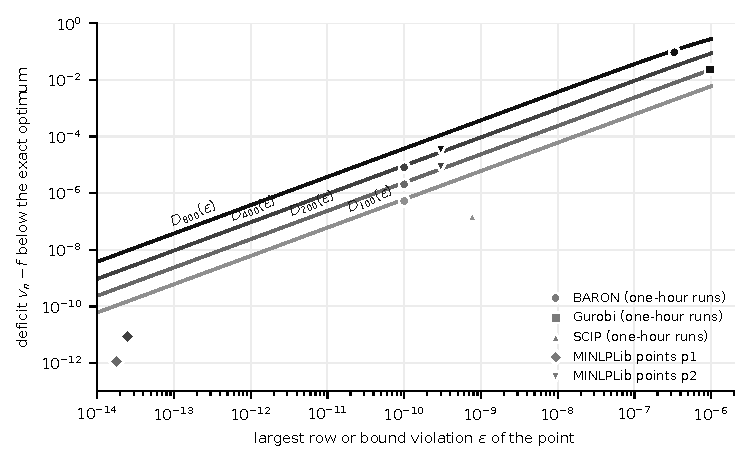
\includegraphics[width=0.9\textwidth]{fig-camshape-deficit.pdf}
\caption{Deficit $v_n-f$ below the exact optimum against the largest row or bound violation $\varepsilon$, for tolerance-feasible points of \inst{camshape<n>}: returned points of the one-hour runs (50-digit evaluation of the savepoints) and MINLPLib's listed points p1 and p2 (exact evaluation), with the proved upper bounds $D_n(\varepsilon)$ of \cref{prop:camshape-deficit}.
The gray level of a marker gives $n$ as for the curves.
No point lies above its curve; BARON's three points at $\varepsilon\approx10^{-10}$ reach about 87\% of $D_n$, and MINLPLib's points p2 about 29\%.
QPLIB's reference points of \inst{QPLIB_2703} and \inst{QPLIB_3177} lie at the positions of the points p2, measured against the optima of these copies.
The curves are computed from the construction of \cref{app:camshape-deficit} in 60-digit arithmetic and agree with \cref{tab:camshape-deficit}.}
\label{fig:camshape-deficit}
\end{figure}

\subsection{Reported values that no exactly feasible point attains}\label{app:solvers-claims}

\Cref{tab:claims} collects the values in category~A of \cref{def:sem-categories} that we checked: values of listed MINLPLib points, the value of the point p2 of \inst{optcdeg2} that MINLPLib lists as Gurobi's dual bound, the two optimality claims and one returned point of our one-hour runs, and published values.
It is not the result of a complete search; \cref{tab:claims-campaign} lists the 15 returned points beyond a certified bound that we evaluated at 50 digits (of 35 such values, \cref{app:solvers-points}).
Each value lies beyond a certified bound or exact optimum (for the KAN instances, the bound for $\Rnet$; for the QPLIB copies, the copy's own bound) or, for \inst{hvycrash}, differs from the objective value $-0.2185$ of every exactly feasible point (\cref{prop:hvycrash-identity}); no exactly feasible point attains it.
For the listed points of \inst{lnts50}, \inst{camshape}, \inst{etamac} and \inst{pricing050}, the value is the objective at the point as we evaluated it; for \inst{etamac} p1 this evaluation has no enclosure, so the value is proved unattainable, but that p1 itself is not exactly feasible is computed (numerical evidence).
The name ``tolerance artifact'' refers to this category; for the \inst{lukvle10} SIF value and Kosolap's \inst{ex6_2_5} value, no violation is reported and the cause is unknown.
Our own floating-point KKT point of \inst{optcdeg2} violates rows by up to $\sci{8.9}{-16}$ and its objective lies at least $\sci{5.95}{-12}$ above $\Uprim$; this says nothing about attainability or about the direction of tolerance effects in general.

% Generated by paper-open-minlplib/data/make_tables.py from data/numbers.json.
% Do not edit by hand; rerun the script. Requires booktabs, array and rotating;
% \inst{} typesets an instance name; underscores are not escaped (macros.tex).
\begin{sidewaystable}
\centering
\scriptsize
\setlength{\tabcolsep}{2pt}
\caption{Reported values that no exactly feasible point attains (category~A; ``tolerance artifact'' names the category, not a diagnosed cause).
Margin: distance to the certified bound $L$ or exact optimum $v^*$ named in the position column (for the QPLIB copies, the copy's own bound), rounded down; page or table displays are first widened by half a unit of their last digit, the QPLIB values by one unit.
Value: the number as reported, except for the listed points of \inst{lnts50}, \inst{camshape}, \inst{etamac} and \inst{pricing050} and for the one-hour runs, whose value is the objective at the point as we evaluated it, exactly except for \inst{etamac} and the one-hour runs (ordinary evaluations without an enclosure; numerical evidence).
Violation: largest row or bound violation of the reported point, where known.
One-hour runs: the two optimality claims and the SCIP point on \inst{camshape100}; of the 35 returned values beyond a certified bound (\cref{app:solvers-points}), \cref{tab:claims-campaign} lists the 15 that we evaluated at 50 digits, 12 of them not repeated here.}
\label{tab:claims}
\begin{tabular}{@{}>{\raggedright\arraybackslash}p{2.8cm}>{\raggedright\arraybackslash}p{3.3cm}>{\raggedright\arraybackslash}p{3.4cm}>{\raggedright\arraybackslash}p{2.9cm}>{\raggedright\arraybackslash}p{1.9cm}>{\raggedright\arraybackslash}p{2.6cm}>{\raggedright\arraybackslash}p{1.9cm}>{\raggedright\arraybackslash}p{4.2cm}@{}}
\toprule
source & model & claim & value & margin & position & violation & qualifier \\
\midrule
MINLPLib point & \inst{lnts50} & p1 & $0.55466876489565$ & $\ge4.30\cdot10^{-11}$ & below $v^*$ & $9.1\cdot10^{-10}$ & exact objective $N h$ of p1 \\
MINLPLib point & \inst{camshape200} & p1 & $-4.27850023299386$ & $\ge1.1\cdot10^{-12}$ & below $v^*$ & $1.8\cdot10^{-14}$ & exact evaluation, agreed by three codes \\
MINLPLib point & \inst{camshape400} & p1 & $-4.27568847893424$ & $\ge8.6\cdot10^{-12}$ & below $v^*$ & $2.5\cdot10^{-14}$ & exact evaluation, agreed by three codes \\
MINLPLib point & \inst{camshape400} & p2 & $-4.27569663342025$ & $\ge8.15\cdot10^{-6}$ & below $v^*$ & $3\cdot10^{-10}$ & exact evaluation, agreed by three codes \\
MINLPLib point & \inst{camshape800} & p2 & $-4.27430686622631$ & $\ge3.27\cdot10^{-5}$ & below $v^*$ & $3\cdot10^{-10}$ & exact evaluation, agreed by three codes \\
MINLPLib point & \inst{hvycrash} & p1 & $-0.21413$ & $\ge0.00436$ & above $v^*=-0.2185$ & $4\cdot10^{-8}$ & objective is constant on $\feas$ \\
MINLPLib point & \inst{hvycrash} & p2 & $-0.21413$ & $\ge0.00436$ & above $v^*=-0.2185$ & $6\cdot10^{-10}$ & objective is constant on $\feas$ \\
MINLPLib point & \inst{etamac} & p1 & $-15.2946756434628$ & $\ge9.46\cdot10^{-11}$ & below $L$ & $1.33\cdot10^{-10}$ & objective evaluated without an enclosure (numerical evidence) \\
MINLPLib point & \inst{pricing050} & p1 & $-1813.8290784498354$ & $\ge2.13\cdot10^{-9}$ & above $L$ (max.) & $7.3\cdot10^{-10}$ & exact objective, printed in binary64 \\
MINLPLib point & \inst{emfl050_3_3} & p2, best primal & $10.40173793$ & $\ge1.41\cdot10^{-5}$ & below $v^*$ & $2\cdot10^{-10}$ & every listed dual valid; marked solved \\
MINLPLib point & \inst{emfl050_5_5} & p6, best primal & $18.91165289$ & $\ge0.00198$ & below $v^*$ & $10^{-8}$ & every listed dual valid \\
MINLPLib point & \inst{emfl100_3_3} & p4, best primal & $18.13236088$ & $\ge2.92\cdot10^{-4}$ & below $v^*$ & $10^{-8}$ & every listed dual valid \\
MINLPLib point & \inst{emfl100_5_5} & p1, best primal & $32.63818348$ & $\ge6.86\cdot10^{-6}$ & below $v^*$ & $10^{-10}$ & every listed dual valid; marked solved \\
one-hour runs & \inst{camshape100} & BARON optimality claim & $-4.284147647561$ & $\ge5.25\cdot10^{-7}$ & below $L$ & $10^{-10}$ & valid dual; tolerance-level closure \\
one-hour runs & \inst{camshape200} & BARON optimality claim & $-4.2785022857$ & $\ge2.05\cdot10^{-6}$ & below $L$ & $10^{-10}$ & valid dual; tolerance-level closure \\
one-hour runs & \inst{camshape100} & SCIP returned point & $-4.284147273656$ & $\ge1.51\cdot10^{-7}$ & below $L$ & $7.7\cdot10^{-10}$ &  \\
MINLPLib (Gurobi) & \inst{optcdeg2} & listed dual = value of p2 & $292.4171346$ & $\ge1.45$ & below $L$ & $10^{-6}$ & the listed dual bound is valid \\
CUTEst SIF & \inst{lukvle10} & SOLTN & $352.237$ & $\ge0.00102$ & below $L$ & not reported & cause unknown; violation not reported \\
Karia et al.\ (SCIP 9.0.1) & \inst{kan_r3_h1_n4} ($\Rnet$) & optimum, gap 0 & $0.00108116412047821$ & $\ge0.00170$ & below $L$ for $\Rnet$ & about $10^{-6}$ & valid as duals of the infeasible OSIL model \\
Karia et al.\ (SCIP 9.0.1) & \inst{kan_r3_h1_n5} ($\Rnet$) & optimum, gap 0 & $-0.0130809958982354$ & $\ge0.00203$ & below $L$ for $\Rnet$ & about $10^{-6}$ & valid as duals of the infeasible OSIL model \\
Karia et al.\ (ConvexHull) & \inst{kan_r5_h1_n5} ($\Rnet$) & primal value & $0.2725188$ & $\ge6.44\cdot10^{-5}$ & below $L$ for $\Rnet$ & not reported &  \\
Kosolap (2019) & \inst{ex6_2_5} & reported optimum & $-70.9586$ & $\ge0.206$ & below $L$ & not reported & cause unknown; violation not reported \\
CAMINO (S-B-MIQP) & \inst{eg_disc2_s} & recorded objective & $5.642100351878204$ & $\ge2.22\cdot10^{-7}$ & below $L$ & not recorded &  \\
GAMS World & \inst{eg_int_s} & old point (objvar) & $6.4531031527$ & $\ge2.33\cdot10^{-10}$ & below $L$ & $6.37\cdot10^{-9}$ &  \\
MINOTAUR 0.4.1 (QPLIB benchmark) & \inst{QPLIB_3177} (copy of \inst{camshape800}) & global optimum & $-4.2774$ & $\ge0.00311$ & below the copy's bound & $>8\cdot10^{-9}$ needed & assumes .nl = .gms \\
ANTIGONE 1.1 (QPLIB benchmark) & \inst{QPLIB_2738} (copy of \inst{camshape100}) & global optimum & $-4.284302$ & $\ge1.54\cdot10^{-4}$ & below the copy's bound & $>2.5\cdot10^{-8}$ needed &  \\
\bottomrule
\end{tabular}
\end{sidewaystable}


\subsection{BARON's claims and the QPLIB copies}\label{app:solvers-baron}

\paragraph{BARON.}
BARON's \inst{camshape100} run needed three iterations and 0.45\,s of solver time, its \inst{camshape200} run 23.22\,s.
Evaluated exactly from the binary64 levels in the savepoints, the returned points have the objective values $-4.28414764756144$ and $-4.27850228570019$ (to the printed digits), largest row violations $\sci{9.995}{-11}$ and $\sci{9.998}{-11}$ (rows \texttt{e100} and \texttt{e200}), and largest bound violations $\sci{9.997}{-11}$ and $\sci{9.998}{-11}$, both on the upper bound of $r_1$; a separate 50-digit evaluation gives the same residuals.

\begin{certbox}[Certificate for \cref{prop:baron-camshape}]
\certitem{Inputs}{OSIL \inst{camshape100} \texttt{9e17da72f0cfe538} and \inst{camshape200} \texttt{76d6141d111fb1a0}; GAMS files \texttt{7f9ef5412da5bb12} and \texttt{fbf6546260555d96}; BARON savepoints \texttt{a243947945113686} and \texttt{b3bb57abdbbbba70}; BARON logs and traces.}
\certitem{Computation}{exact optima of \cref{thm:camshape-opt}; exact evaluation of objective and residuals at the savepoint levels; subtraction \arith{E}.}
\certitem{Data reading}{exact decimals of the model files; savepoint levels as exact binary64 values.}
\certitem{Implementations}{the bound: those of \cref{thm:camshape-opt}; the evaluation: one exact code and one 50-digit code.}
\certitem{Evidence level}{\evid{stored}.}
\certitem{Replay}{Tier~1; seconds.}
\end{certbox}

\begin{proposition}[Reported optima of the rounded copies]\label{prop:qplib-copies}
Read \inst{QPLIB_3177} (the copy of \inst{camshape800}) and \inst{QPLIB_2738} (the copy of \inst{camshape100}) with exact decimals.
In Mittelmann's QPLIB benchmark \citep{mittelmann2026-continuous-non-convex-qplib-benchmark}, MINOTAUR~0.4.1 reports the optimal value $-4.2774$ for \inst{QPLIB_3177}, and ANTIGONE~1.1 the global minimum $-4.284302$ for \inst{QPLIB_2738}.
\textup{(a)}~No exactly feasible point of the copy attains any number within one unit of the last displayed digit of the reported value; the margins are at least $\sci{3.11}{-3}$ and $\sci{1.54}{-4}$.
\textup{(b)}~Every point of \inst{QPLIB_3177} with objective below $-4.2773$ violates some row or bound by more than $\sci{8}{-9}$, and every point of \inst{QPLIB_2738} with objective below $-4.284301$ violates some row or bound by more than $\sci{2.5}{-8}$.
For MINOTAUR, which read \inst{QPLIB_3177} in AMPL's \texttt{.nl} format, we assume that this file has the rows and bounds of the GAMS copy.
\end{proposition}

\begin{proof}
By \cref{prop:camshape-copies}, the optimal values of the copies are at least $-4.2741871514717434$ and $-4.2841462678046117$.
Every number within one unit of the last displayed digit of $-4.2774$ is below $-4.2773$, and every such number for $-4.284302$ is below $-4.284301$; subtraction gives~(a).
For~(b), \cref{app:camshape-copies} applies the construction of \cref{prop:camshape-deficit} to the copies: points with violations of at most $\sci{8}{-9}$ (\inst{QPLIB_3177}) and $\sci{2.5}{-8}$ (\inst{QPLIB_2738}) have objective values at least $-4.2771731888$ and $-4.2842973949$.
These lie above the thresholds $-4.2773$ and $-4.284301$ by more than $10^{-6}$, so the conclusion holds even if an objective row is also violated by the same amount.
If the reported values are roundings to nearest, the thresholds become $-4.27735$ and $-4.2843015$, and (a) and (b) hold a fortiori.
\end{proof}

The dual bounds implied by the two claims equal the reported values and are valid, so both values are tolerance artifacts on the copies (category~A); points built in floating point reach them with violations of $\sci{9.7}{-9}$ and $\sci{2.9}{-8}$ (numerical evidence).

\paragraph{The QPLIB runs.}
MINOTAUR~0.4.1 read \texttt{QPLIB\_3177.nl} in Mittelmann's benchmark, with eight threads and a limit of 10800\,s; its log reports one processed node, the best value $-4.2774$, a bound of $+\infty$ from the remaining nodes and ``Optimal solution found'' after 2.89\,s.
We did not obtain the \texttt{.nl} file.
ANTIGONE~1.1 read \texttt{QPLIB\_2738.gms.gz} under GAMS~52.3.0 with an option file that only names a CPLEX option file, whose contents are not recorded; its log reports ``Global minimum'' with best feasible and best possible values $-4.284302$ and relative gap $10^{-9}$.
In the same benchmark, SCIP~9.2.1 stopped on \inst{QPLIB_2703} at its time limit with the incumbent $-4.33023953971002$, at least $\sci{5.45}{-2}$ below the copy's optimum; it read the copy in LP format, which we assume encodes the same model.

\begin{certbox}[Certificate for \cref{prop:qplib-copies}]
\certitem{Inputs}{GAMS copies \inst{QPLIB_2738} \texttt{b30f282782e78cb9} and \inst{QPLIB_3177} \texttt{4d0e595fdd62b995}; MINOTAUR log \texttt{ffed0cd9294ed4e4}; ANTIGONE log \texttt{a691f994f3e81a34}.}
\certitem{Computation}{exact optima of the copies (\cref{prop:camshape-copies}) and their tolerance versions at the two values of $\varepsilon$, in exact rational arithmetic with upper bounds rounded up to a fixed grid \arith{E}; subtraction.}
\certitem{Data reading}{exact decimals of the GAMS copies; each parser asserts complete tokenization and the row structure.}
\certitem{Implementations}{besides those of \cref{prop:camshape-copies}, three codes from three agent sessions compute the comparison lower bound of all four copies and agree to 20 digits; two of them reproduce the two tolerance bounds. MINOTAUR's input is assumed equal to the GAMS copy.}
\certitem{Evidence level}{\evid{stored}.}
\certitem{Replay}{Tier~1; under one minute.}
\end{certbox}

\subsection{The SCIP defect}\label{app:solvers-scip}

\paragraph{Versions.}
We tested SCIP~10.0.2 through PySCIPOpt~6.2.1 and as the official binary (commit \texttt{b8eaf989f9}); SCIP~10.0.3 as the official binary and through GAMS~54.3.1 (commit \texttt{d409edf9f6}); SCIP~10.1.0 as the official binary (commit \texttt{c8e5737a84}, released 2026-09-18); and a local build of the development branch at commit \texttt{a01de2c} (2026-10-02, version string 11.0.0).
Debug builds of 10.0.2 and of the development snapshot, with the debugging-solution mechanism and a small diagnostic patch, served for tracing.
All runs were on Ubuntu~24.04 (x86-64).

\paragraph{Models.}
The models p0, p4 and p5 are the single-period Lagrangian subproblems of \inst{waterno2_06} for periods 0, 4 and~5 (166 variables, 9 of them binary, and 203 rows), with the multipliers of our period decomposition (\cref{sec:split-waterno2}); each row is an exact copy of the same-named OSIL row.
The model \inst{pair2236} restricts the period-3 subproblem to one pair of cells by 17 variable bounds.
Each pump station has a binary $b$, a speed $s\in[\ell,1]$, a squared speed $q=s^2$ and a power $p=s^3$, with bounds $q\ge \ell^2$ and $p\ge \ell^3$ written as exact decimals and a speed row $s-(1-\ell)b\le \ell$; when $b=0$, the rows force $s=\ell$ and $p=\ell^3$.
The values $\ell\in\{0.6,0.7,0.8,0.85\}$ occur in every period.
The model \inst{fm336} has 15 variables and 12 rows, with pumps $i=0,1,2$ and $(\ell_0,\ell_1,\ell_2)=(0.7,0.85,0.6)$:
\begin{align*}
\min\quad & 5w_0+0.2\,b_1+w_1+0.1\,b_2+2w_2\\
\text{s.t.}\quad & p_0=s_0^3,\quad p_2=s_2^3,\\
& s_0-0.3\,b_0\le0.7,\quad s_1-0.15\,b_1\le0.85,\quad s_2-0.4\,b_2\le0.6,\\
& q_0-3s_0-0.3\,b_0\le-2.1,\quad q_1-2s_1-0.3\,b_1\le-1.7,\quad q_2-3s_2-0.3\,b_2\le-1.8,\\
& w_i-p_i-b_i\ge-1\ (i=0,1,2),\qquad q_0+q_1+q_2\ge0.5,\\
& s_0\in[0.7,1],\ s_1\in[0.85,1],\ s_2\in[0.6,1],\ p_0\in[0.343,1],\ p_1\in[0.614125,0.614125],\\
& p_2\in[0.216,1],\ q_0,q_1\in[0,1],\ q_2\in[0,0.5],\ w_i\in[0,1],\ b_i\in\{0,1\}.
\end{align*}
We call the rows with $q_i$ flow rows and the row $q_0+q_1+q_2\ge0.5$ the demand row.
The model \inst{tiny2} is $\min\ 0.2\,b-2.4\,s+p$ subject to $p=s^3$, $s-0.3\,b\le0.7$, $b\in\{0,1\}$, $s\in[0.7,1]$, $p\in[0.343,1]$.
The models \inst{pumps_default} (20 variables, 12 rows) and \inst{fm318} (10 variables, 8 rows) have the same structure.

\paragraph{Wrong runs.}
A run counts as wrong if SCIP reports an optimal solution with a dual bound that exceeds the witness value by more than $10^{-4}$.
\Cref{tab:scip-runs} counts the wrong runs; only the seed shift \texttt{randomization/\allowbreak randomseedshift} varies, and all other settings are defaults, except that \inst{tiny2} is solved wrongly only with heuristics and separation switched off (with default settings every version returns $-1.337$).
\Cref{tab:scip-witnesses} lists the witnesses and the range of wrong values.

\begin{table}[t]
\centering
\scriptsize
\setlength{\tabcolsep}{3pt}
\caption{Wrong runs per model and SCIP version, out of the seeds tried, under default settings (\inst{tiny2}: heuristics and separation off). PySCIPOpt runs SCIP~10.0.2 and GAMS runs SCIP~10.0.3; ``dev'' is the development snapshot \texttt{a01de2c}; ``dbg'' is the 10.0.2 debug build. Solver output.}
\label{tab:scip-runs}
\begin{tabular}{@{}lrrrrrrr@{}}
\toprule
model & PySCIPOpt & 10.0.2 & 10.0.3 & 10.1.0 & dev & GAMS & dbg \\
\midrule
p0 & 4/20 & 4/10 & 4/10 & 2/10 & 0/10 & 3/3 & -- \\
p4 & 19/20 & 8/10 & 8/10 & 10/10 & 9/10 & 10/10 & 8/10 \\
p5 & 13/20 & 4/10 & 4/10 & 5/10 & 4/10 & 1/3 & -- \\
\inst{pair2236} & 7/30 & 8/30 & 8/30 & 5/30 & 5/30 & 1/10 & 4/30 \\
\inst{pumps_default} & 20/20 & 10/10 & 10/10 & 10/10 & 1/20 & 0/5 & traced \\
\inst{fm336} & 10/10 & 10/10 & 10/10 & 10/10 & 10/10 & 5/5 & 10/10 \\
\inst{fm318} & 0/10 & 0/10 & 0/10 & 0/10 & 10/10 & 0/5 & 0/10 \\
\inst{tiny2} & wrong & wrong & wrong & wrong & wrong & wrong & wrong \\
\bottomrule
\end{tabular}
\end{table}

\begin{table}[t]
\centering
\footnotesize
\caption{Exactly feasible witnesses and the wrong optimal values that they refute. Witness values are exact or rounded up; wrong values are SCIP output, rounded to six decimals.}
\label{tab:scip-witnesses}
\begin{tabular}{@{}lllll@{}}
\toprule
model & variables/rows & witness value & smallest wrong value & largest wrong value \\
\midrule
p0 & 166/203 & $168.108652029808$ & $169.950250$ & $169.950685$ \\
p4 & 166/203 & $-6.730643699816$ & $-6.729889$ & $-4.646232$ \\
p5 & 166/203 & $-232.172853003462$ & $-231.905843$ & $-228.343114$ \\
\inst{pair2236} & 166/203 & $55.689908409450$ & $56.492038$ & $65.124528$ \\
\inst{tiny2} & 3/2 & $-1337/1000$ & $-1.231084$ & $-1.231084$ \\
\inst{pumps_default} & 20/12 & $153/250$ & $1.198000$ & $1.198000$ \\
\inst{fm336} & 15/12 & $187/270$ & $0.814125$ & $1.505213$ \\
\inst{fm318} & 10/8 & $729/500$ & $2$ & $2$ \\
\bottomrule
\end{tabular}
\end{table}

\paragraph{Witnesses.}
Each witness is a rational point: for p0, p4 and p5 a repaired near-optimal point of our period decomposition, for \inst{pair2236} a point whose binaries are fixed and whose other variables are solved exactly from the equality rows, and for the small models an explicit rational point.
The witness of \inst{fm336} is $b=(0,0,1)$, $s=(7/10,17/20,2/3)$, $p=(343/1000,4913/8000,8/27)$, $q=(0,0,1/2)$, $w=(0,0,8/27)$, with objective value $0.1+2\cdot8/27=187/270$; that of \inst{tiny2} is $b=0$, $s=7/10$, $p=343/1000$.
Each witness was checked in exact rational arithmetic by six to eight checkers, from eight code bases written in six agent sessions: four to six read the CIP file or the model specification, and two read the GAMS file. All report no violated row, bound or integrality condition, and perturbing a coordinate by $10^{-30}$ or a binary by $1/2$ is detected.
Besides the acceptance and the binary64 residuals stated in \cref{prop:scip-witnesses}, SCIP~10.0.2, 10.0.3, 10.1.0 and the development snapshot accept the \inst{fm336} witness when it is read as a solution file and then report $0.692592587925926$ as optimal.

% The binary64 residual bound 2.93e-15 of prop:scip-witnesses is the exact maximum
% 32122061/10995116277760000000000 = 2.9214844...e-15 over the four large witness/model
% pairs, recorded in development/reviews/round1/sol-numbers.md:34-40 (round-2 G6-05).
\begin{certbox}[Certificate for \cref{prop:scip-witnesses}]
\certitem{Inputs}{CIP models p0 \texttt{18bfbf2a6696c984}, p4 \texttt{7fb721e5174f1f2b}, p5 \texttt{4d56b776d1fda19d}, \inst{pair2236} \texttt{29b742c4f232074a}, \inst{tiny2} \texttt{5e16aa0407566ff3}, \inst{pumps_default} \texttt{6fa5108c7240e2fc}, \inst{fm336} \texttt{eac0b3ab0f7dc4cb}, \inst{fm318} \texttt{b960024133f52d3a}; witnesses of p0, p4, p5, \inst{pair2236}, \inst{fm336}: \texttt{9ea1bbf28b23e438}, \texttt{e25f87ed2be1ce85}, \texttt{4b621394ab17c9a6}, \texttt{8226628f7704a134}, \texttt{bddd287e1a6543d1}; the matching GAMS files; SCIP logs.}
\certitem{Computation}{exact evaluation of every row, bound and integrality condition \arith{E}; comparison with the reported values.}
\certitem{Data reading}{exact decimals of the CIP and GAMS files.}
\certitem{Implementations}{six to eight exact checkers per witness (eight code bases from six agent sessions), two of them reading the GAMS files.}
\certitem{Evidence level}{\evid{stored}; acceptance by SCIP is solver output.}
\certitem{Replay}{Tier~1; seconds.}
\end{certbox}

\begin{proposition}[The reproducers in three senses]\label{prop:scip-reproducers}
\textup{(a)}~The optimal value of \inst{fm336} is $187/270$, and that of \inst{tiny2}, a model with one pump, is $-1.337$.
\textup{(b)}~SCIP's optimal values for \inst{fm336}, $1.50521312595154$ in the releases and $0.814125$ in most seeds of the development snapshot, are wrong in three senses.
(1)~Decimal data read exactly, zero tolerance (as in \reading{b}): they exceed the optimal value, so SCIP's dual bound is invalid.
(2)~SCIP's own tolerances: SCIP accepts the optimal point, whose value is lower by $0.12$ to $0.81$, so its output is inconsistent.
(3)~Binary64 data, zero tolerance (as in \reading{c}): every feasible point costs more than $2.247$, so the dual bound is valid, but the returned points are infeasible and the reported value is not optimal.
\end{proposition}

\begin{proof}
(a)~Every objective term of \inst{fm336} is nonnegative, and the rows $w_i-p_i-b_i\ge-1$ give $w_i\ge p_i$ when $b_i=1$.
If $b_1=1$, the cost is at least $0.2+w_1\ge0.2+p_1=0.814125$.
If $b_0=1$, then $w_0\ge p_0\ge0.343$ and the cost is at least $1.715$.
Otherwise $b_0=b_1=0$, the speed rows and bounds force $s_0=0.7$ and $s_1=0.85$, the flow rows give $q_0\le0$ and $q_1\le0$, and the demand row forces $q_2\ge0.5$.
If also $b_2=0$, then $s_2=0.6$ and $q_2\le0$, which is infeasible.
So $b_2=1$, the flow row gives $3s_2\ge q_2+1.5\ge2$, and $w_2\ge p_2=s_2^3\ge8/27$, so the cost is at least $0.1+16/27=187/270$, which the witness attains.
For \inst{tiny2}, $b=0$ forces $s=0.7$, $p=0.343$ and the value $-1.337$.
If $b=1$, the minimum of $0.2-2.4s+s^3$ over $[0.7,1]$ is attained at $s=\sqrt{0.8}$ and equals $0.2-1.6\sqrt{0.8}$, which exceeds $-1.337$ because $0.8<(1.537/1.6)^2=0.922800390625$.

(b)~With the decimal data read exactly, the reported values $0.814125$ and $1.50521312595154$ exceed $187/270$; SCIP's dual bound, which equals the reported value within SCIP's default gap limits, is therefore invalid.
Under SCIP's tolerances, SCIP accepts the witness, whose value is $187/270$, which contradicts its claim of a larger optimal value.
With binary64 data and zero tolerance, $b_0=0$ forces $s_0=\fl(0.7)$ and $p_0=\fl(0.7)^3<\fl(0.343)$ (\cref{lem:scip-cube}), which violates the lower bound of $p_0$; likewise $b_2=0$ forces $p_2=\fl(0.6)^3<\fl(0.216)$.
So every feasible point has $b_0=b_2=1$, hence $w_0\ge p_0\ge\fl(0.343)$ and $w_2\ge p_2\ge\fl(0.216)$, and costs at least $5\fl(0.343)+\fl(0.1)+2\fl(0.216)$, which exact rational arithmetic shows to exceed $2.247$.
SCIP's dual bound is then valid.
Its returned points, whose values lie below $5\fl(0.343)$, have $b_0=0$; so they are infeasible, and the reported value is not the optimal value.
For \inst{tiny2} the same reading excludes $b=0$; the optimal value is then $0.2-1.6\sqrt{0.8}$ up to data rounding, which SCIP's value $-1.23108446311479$ undercuts by about $\sci{9.6}{-7}$, so \inst{tiny2} shows an error only in senses (1) and~(2).
\end{proof}

\begin{lemma}[The data trigger]\label{lem:scip-cube}
Let $a=\fl(0.343)-2^{-53}$ and $b=\fl(0.343)-2^{-54}$.
Then $a<\fl(0.7)^3<b$, so $[a,b]$ is the tightest interval with binary64 ends that contains $\fl(0.7)^3$, and it lies below $\fl(0.343)$.
For the other station values $\ell$ of \inst{waterno2} ($0.6$ and $0.85$ for squares and cubes, $0.7$ for squares, and the upper bound $0.8$ for squares and cubes), the tightest such interval around $\fl(\ell)^k$ contains $\fl(\ell^k)$.
\end{lemma}

\begin{proof}
The binary64 numbers in $[0.25,0.5)$ are spaced $2^{-54}$ apart, and $\fl(0.343)$ lies in this range, so $a$ and $b$ are its two predecessors.
Exact rational arithmetic gives $\fl(0.7)^3-\fl(0.343)\approx\sci{-9.2371}{-17}$, which lies strictly between $-2^{-53}$ and $-2^{-54}$; hence $a<\fl(0.7)^3<b<\fl(0.343)$.
In shortest round-trip form, $a$ and $b$ print as $0.3429999999999999$ and $0.34299999999999997$; $\fl(0.343)$ exceeds $0.343$ by about $\sci{2.7}{-17}$.
For the other cases the residuals $\fl(\ell)^k-\fl(\ell^k)$ are about $\sci{-1.3323}{-17}$ ($0.6^2$), $\sci{-2.1538}{-17}$ ($0.6^3$), $\sci{-5.3291}{-17}$ ($0.7^2$), $\sci{-6.8834}{-17}$ ($0.85^2$), $\sci{-8.0103}{-17}$ ($0.85^3$), $\sci{5.7732}{-17}$ ($0.8^2$) and $\sci{7.4607}{-17}$ ($0.8^3$).
Each is smaller in absolute value than the spacing of the binary64 numbers on the relevant side of $\fl(\ell^k)$ ($2^{-55}$ below $0.216$, $2^{-54}$ below $0.36$ and $0.49$, $2^{-53}$ next to $0.512$, $0.614125$, $0.64$ and $0.7225$), so $\fl(\ell^k)$ is an end of the tightest enclosure of $\fl(\ell)^k$.
Three separately written exact computations agree on these values; each takes under a second.
\end{proof}

\begin{certbox}[Certificate for \cref{lem:scip-cube}]
\certitem{Inputs}{the decimal strings $0.6$, $0.7$, $0.8$, $0.85$ and their squares and cubes as written in the \inst{waterno2} files.}
\certitem{Computation}{binary64 values of the strings, their exact powers, residuals and neighbouring binary64 numbers, in exact rational arithmetic \arith{E}.}
\certitem{Data reading}{correctly rounded decimal-to-binary64 conversion (\cref{hyp:fp-ieee}).}
\certitem{Implementations}{three separately written exact computations agree.}
\certitem{Evidence level}{\evid{stored}.}
\certitem{Replay}{Tier~1; under a second.}
\end{certbox}

\paragraph{The traced steps.}
A trace of \inst{tiny2} in the 10.0.2 debug build shows the mechanism.
SCIP branches on $b$ at the root; at the node $b=0$:
\begin{enumerate}
\item Linear propagation fixes $s=\fl(0.7)$.
\item In the first round of nonlinear propagation the outward activity of $s^3$ is $[\fl(0.343)-3\cdot2^{-54},\,b]$, printed as $[0.34299999999999986,\,0.34299999999999997]$.
Reverse propagation of $s^3-p\in[0,0]$ gives $p\le b$, which lies $2^{-54}$ below the lower bound $\fl(0.343)$ of $p$; SCIP accepts this within its tolerance and fixes $p=\fl(0.343)$.
\item In the next round both variables are fixed, and the default setting \texttt{r} of \texttt{constraints/\allowbreak nonlinear/\allowbreak varboundrelax} relaxes each bound by $\min(\epsilon\max(1,|\text{bound}|),\,0.001(\text{ub}-\text{lb}))$, which is zero for a fixed variable.
The default nonlinear handler propagates the sum backward through \texttt{SCIPinterval\allowbreak PropagateWeightedSum}, which intersects the activity $[-3\cdot2^{-54},-2^{-54}]$ of $s^3-p$ with $[0,0]$ by the exact routine \texttt{SCIPintervalIntersect}; only its upper end $b-\fl(0.343)$ (\cref{lem:scip-cube}) matters for the cutoff, and the lower end is looser than the tightest enclosure.
The intersection is empty, the node is declared infeasible, $b\ge1$ becomes a global bound and SCIP returns $-1.23108446311479$ as optimal.
\end{enumerate}
The same discrepancy of $2^{-54}$ is accepted in one round and fatal in the next.
Most intersections in the nonlinear constraint handler and the default nonlinear handler use the $\varepsilon$-tolerant \texttt{SCIPintervalIntersectEps}; this one does not.
In the root cutoffs of \inst{fm336}, \inst{fm318} and \inst{pumps_default}, SCIP first finds an incumbent, then fixes a pump binary to~0 by valid propagation, and the next nonlinear round declares the root infeasible; SCIP returns the incumbent as optimal.
In \inst{fm336} the node declared infeasible contains SCIP's own incumbent, which also has $b_0=0$.

\paragraph{Instrumented runs and settings.}
The 15 instrumented wrong runs, eight in the 10.0.2 debug build and seven in that of the development snapshot, cover all eight models.
In each, the first report that the witness was cut off, or the first invalid bound, follows the infeasibility declaration of \cref{obs:scip-propagation} on a cube row of a $0.7$ station.
The run of \inst{pair2236} with seed shift~11 was not instrumented: the debug build records its first invalid implication, which fixes a binary of a $0.85$ station, but not the step that caused it; at that station the tightest enclosure of the cube meets the bound (\cref{lem:scip-cube}), so the traced mechanism does not explain this run.
Two wrong runs of p4 have small excesses, about $\sci{7.5}{-4}$ and $\sci{8.9}{-4}$; in the first, SCIP's solution has a pump configuration different from the witness's, so a subtree was lost.
Neither debug build reproduces these two runs, and they were not traced.
With the setting \texttt{b} of \texttt{varboundrelax}, which relaxes all bounds by $\epsilon$, including fixed ones, the wrong runs fell from 78 of 122 to none, in four groups: PySCIPOpt on p0, p4, p5 and \inst{pair2236} (27/60), the wrong runs of the development snapshot and one more (19/20), \inst{fm336} and \inst{fm318} in the development snapshot and 10.1.0 (30/40), and the two small-excess runs (2/2).
This links the runs that could not be instrumented (PySCIPOpt, official binaries, GAMS) to the mechanism only as evidence.
On \inst{fm336} the error also disappears when nonlinear propagation is switched off, with the settings \texttt{a} or \texttt{n} of \texttt{varboundrelax}, or with the feasibility tolerance $10^{-9}$, but not when OBBT, reduced-cost fixing, probing, conflict analysis, symmetry handling or restarts are switched off; some of these changes may only alter the search path.
Why the setting \texttt{n}, which does not relax fixed variables either, avoids the cutoff was not determined, and no change to the source code was tested.

\paragraph{The data trigger in MINLPLib.}
A scan of the 1,632 OSIL files of the MINLPLib snapshot (every instance except \inst{fct}, whose page offers no OSIL file; \cref{app:audit-screen}) looks for equality rows $y-x^k=0$ ($k\in\{2,3\}$; one power, square, product or quadratic term plus one linear term; zero right-hand side) with $\mathrm{lb}(y)=\mathrm{lb}(x)^k$ or $\mathrm{ub}(y)=\mathrm{ub}(x)^k$ in decimal and a binary64 residual of the infeasible sign.
Rows of this form that agree in decimal occur in twelve instances; in three \inst{kall_ellipsoids} instances they also agree in binary64.
Rows with the infeasible binary64 sign occur only in \inst{waterno2_01}, \inst{waterno2_02}, \inst{waterno2_03}, \inst{waterno2_04}, \inst{waterno2_06}, \inst{waterno2_09}, \inst{waterno2_12}, \inst{waterno2_18} and \inst{waterno2_24}, at the stations $0.6$, $0.7$ and $0.85$ (lower bounds) and $0.8$ (upper bound); by \cref{lem:scip-cube}, only the cube rows at the $0.7$ stations, one per period, have an enclosure that misses the bound.
The scan is syntactic: it misses scaled forms $y=a\,x^k$, bounds implied by other rows and other functions, and it does not test whether SCIP's search reaches the fixed state.
The listed SCIP bounds of \inst{waterno2_01} and \inst{waterno2_02} agree with several other solvers on instances marked solved.
On \inst{waterno2_03} and \inst{waterno2_04}, which are not marked solved, the listed SCIP bounds (dated 2022-02-15) equal the listed primal values and exceed the listed bounds of LINDO and BARON by at most $\sci{5.7}{-5}$ and $\sci{3.71}{-4}$; if those bounds are valid, this limits how far the SCIP bounds can be too high.
We examined neither further.

\paragraph{Optimal values of the subproblems.}
The branch and bound of our \inst{waterno2} certificates (\cref{app:waterno2}) proves, with the same multipliers, that the optimal values of p0, p4, p5 and \inst{pair2236} are at least $168.107652$, $-6.731984$, $-232.173990$ and $55.0942345$.
With the witnesses, the optimal values thus lie in intervals of width at most $\sci{1.4}{-3}$ (periods) and $0.6$ (cell pair).
Every wrong value of \cref{tab:scip-witnesses} lies above its interval; SCIP's low values $55.689773$ and $55.689858$ on \inst{pair2236} lie inside and are neither refuted nor confirmed.

\paragraph{Related reports.}
A search of the SCIP issue tracker on 2026-10-02 found no matching report; this does not show that none exists.
Issues \#162 (a suboptimal result on multilinear relations) and \#190 (presolving that renders a problem infeasible) report wrong results on nonlinear models, but their discussions point to other causes; issue \#22 (a second-order cone program reported infeasible by SCIP~8) is a similar kind of error with no common cause shown.
The archive contains \inst{fm336} and \inst{tiny2} in CIP and GAMS form, with exact witnesses and solution files.
As of 2026-10-05, we have not yet reported the defect to the SCIP developers.

\subsection{Inputs of the published claims}\label{app:solvers-published}

\paragraph{CAMINO.}
\Cref{sec:solvers-invalid} proves \cref{prop:camino-eg} from the points of \cref{app:eg}; here we record its inputs.
We use the file \texttt{noncvx\_gurobi.csv} of the CAMINO data \citep{ghezzi2026-camino-benchmark-results-for-nonconvex} at commit \texttt{66a134daf8} (2026-03-19).
The pipeline stores AMPL's \texttt{obj.bestbound} as the dual bound, with per-instance time limits of 32.63\,s, 19.24\,s and 212.66\,s for \inst{eg_disc2_s}, \inst{eg_disc_s} and \inst{eg_int_s}.
The interval evaluation of the AMPL files proves every row with smallest slacks of at least $\sci{7.4}{-20}$, $\sci{7.8}{-20}$ and $\sci{5.5}{-20}$.
The SCIP~9.2.2 bounds in the same data are valid.
Our Gurobi~13.0.2 runs reached the time limit on all three instances with valid final bounds; its log for \inst{eg_int_s} warns that the returned point violates a constraint by $\sci{5.958}{-5}$, more than its own tolerance.

\begin{certbox}[Certificate for \cref{prop:camino-eg}]
\certitem{Inputs}{CAMINO data file \texttt{3d20ec89bb498de2} and pipeline code; AMPL files \texttt{f68aeac9db35e910}, \texttt{7056c8347d233c04}, \texttt{5eec7b71100978e8}; the primal points of \cref{thm:eg-bounds}.}
\certitem{Computation}{interval evaluation of every row, bound and integrality condition at the points \arith{I} (mpmath, 200 bits; $+,-,\times,\div,\exp$); subtraction.}
\certitem{Data reading}{decimal strings enclosed outward by intervals.}
\certitem{Implementations}{one interval checker for the AMPL files; the exact feasibility of the same points for the OSIL models is proved separately (\cref{app:eg}).}
\certitem{Evidence level}{\evid{stored}, assuming that CAMINO's model files equal MINLPLib's and that the recorded bound is AMPL's \texttt{bestbound}.}
\certitem{Replay}{Tier~1; seconds.}
\end{certbox}

\paragraph{MINOTAUR on the copy of \inst{optcdeg2}.}
\Cref{sec:solvers-invalid} proves \cref{prop:minotaur-optcdeg2}; \cref{app:optcdeg2-minotaur} adds what the log shows.
After comment lines are removed, the file \texttt{QPLIB\_8803.gms} (SHA-256 \texttt{6817fc437ad64304}) differs from MINLPLib's \inst{optcdeg2} file (\texttt{42171d55a52aa4ec}) only by a redundant declaration that makes two variables nonnegative which both files fix at~0, the formatting of one option line, and the solve statement; \texttt{QPLIB\_8585.gms} and \inst{dtoc5} differ in the last two respects only.
MINOTAUR's log (\texttt{f12b9bba2e1b51d3}) shows reading (0.64\,s), the first presolve, and ``status of presolve: Detected infeasibility'' after 119\,s of CPU time.
On \inst{QPLIB_3177} the same version starts the quadratic handler, which adds default bounds to unbounded variables, only after this first presolve.
The proposition needs only the exactly feasible point of \inst{optcdeg2} (\cref{prop:optcdeg2-point}), whose certificate it inherits, and the assumption on the \texttt{.nl} file.

\begin{proposition}[Published SCIP optima for two KAN instances]\label{prop:kan-scip}
For \inst{kan_r3_h1_n4} and \inst{kan_r3_h1_n5}, \citet{karia2025-deterministic-global-optimization-over-trained} report SCIP~9.0.1 runs that end with ``optimal solution found'' and gap~0 at $\sci{1.08116412047821}{-3}$ and $\sci{-1.30809958982354}{-2}$ \citep{karia2025-karia-et-al-zenodo-default}.
These values lie at least $\sci{1.70}{-3}$ and $\sci{2.03}{-3}$ below the certified lower bounds $\Lcert$ of \cref{thm:kan-enclosure}, so no point of $\Rnet$ or $\RP$ attains them.
\end{proposition}

\begin{proof}
The displays of $\Lcert$ in \cref{tab:kan}, $0.002781237152581$ and $-0.01104267952179$, are rounded down; subtracting the reported values from them gives the margins.
Since $\Lcert\le\vstar(\Rnet)\le\vstar(\RP)$, no point of either model attains the reported values.
\end{proof}

\paragraph{The KAN models of \citet{karia2025-deterministic-global-optimization-over-trained}.}
Reading the values of \cref{prop:kan-scip} as claims about MINLPLib's models assumes that the published models equal MINLPLib's up to the printing of coefficients.
The published runs solved Pyomo models through the AMPL solver library; their variable, row and integer counts equal MINLPLib's, and an input-order test confirmed the correspondence of the inputs.
Evaluated at 60 digits, the network at the reported inputs of the two zero-gap runs gives $0.0028684784$ and $-0.0108512435$, above the certified bounds.
With the inputs fixed at these points, SCIP~10.0 again reports ``optimal'' values below the certified bounds, with largest row violations $\sci{9.34}{-7}$ and $\sci{9.99}{-7}$.
These evaluations are numerical evidence for the tolerance explanation; the proposition needs only the certified bounds, and it inherits their certificate (\cref{thm:kan-enclosure}, evidence level \evid{rerun}).

% Plan: development/outline.md, section 6, item I. Internal script names
% may appear here, in neutral form.
% Sources: R/publication/reproduction/README.md and commands.json (commands,
% recorded wall times), R/publication/integration/runtime-evidence-r1.json,
% the family dossiers and critiques, development/reviews/*.md,
% development/eg-audit/out/{run_audit,compare}.log (per-instance sums of the
% audited eg run: eg_int_s 465 s, eg_disc_s 1,456 s, eg_disc2_s 14,782 s),
% R/publication/reproduction/water-audit/logs/, R/publication/reproduction/
% network/logs/ann.*.time, development/reviews/round1/kan-guard/ (guarded KAN
% replay) and development/reviews/round1/sol-numbers.md (rocket and GAMS/OSIL
% reruns). Expected outputs point to the generated tables and to
% data/numbers.json. Tiers follow the rule of Section 10 (recorded wall time
% per instance, summed over its parts). Round-1 revision (G7-12): status per
% register row, trust labels defined here, archive layout, setup sequence.
% The stored-model table is generated (tables/tab-sem-hashes.tex).
\section{Reproduction guide and claim register}\label{app:repro}

The files and scripts that replay each result are named here; the main text avoids these names.
As \cref{sec:semantics-protocol} states, AI agents working under the authors' direction wrote the implementations and ran the checks; that section defines ``separately written''.
Paths are relative to the root of the archive (\archiveDOI), which keeps the layout of our working tree, including working folder names such as \nolinkurl{open-instances-wave3/} or \nolinkurl{dossiers/}: \nolinkurl{$R} denotes its folder \nolinkurl{research-20260929/} and \nolinkurl{$P} its folder \nolinkurl{paper-open-minlplib/}.
\Cref{tab:repro-register} lists the replay entry points; times are recorded wall times on a shared machine, and \cref{sec:repro} defines the tiers by these times.

\subsection{Setup}\label{app:repro-setup}

The guide \nolinkurl{$P/artifact/README.md} describes the files of the artifact, the environment, the long replays and the earlier reproduction package in \nolinkurl{$R/publication/reproduction/}.
The checkers need Python~3.13.11 and the package versions pinned in \nolinkurl{$R/publication/reproduction/requirements.txt}; the \inst{dtoc5} checker also needs the GMP library, and the solver campaign needs GAMS~54.3.1 and solver licences.
Several scripts write into their own \nolinkurl{logs/} folders and some replace stored evidence, so every command runs in a disposable copy \nolinkurl{$WORK} of the archive, with at most four single-threaded processes at a time.
A session starts as follows; the unpacked archive \nolinkurl{$ARCHIVE} is only read.
\begin{verbatim}
ARCHIVE=/path/to/unpacked/archive          # read only
WORK=$(mktemp -d /tmp/minlp-work-XXXXXX)   # disposable: rm -rf "$WORK"
cp -r "$ARCHIVE"/. "$WORK"/ && cd "$WORK"
export HOME="$WORK/home" XDG_CACHE_HOME="$WORK/home/.cache"
export TMPDIR="$WORK/tmp" PIP_NO_CACHE_DIR=1 PYTHONDONTWRITEBYTECODE=1
R="$WORK/research-20260929"; P="$WORK/paper-open-minlplib"
export MINLP_REPO_ROOT="$WORK" EG_AUDIT_R="$R" MINLPLIB_OSIL_ROOT="$WORK/osil"
export OMP_NUM_THREADS=1 OPENBLAS_NUM_THREADS=1 MKL_NUM_THREADS=1
export NUMEXPR_NUM_THREADS=1
mkdir -p "$TMPDIR" "$MINLPLIB_OSIL_ROOT" "$HOME/.cache/minlplib/minlplib"
cp "$R"/publication/minlplib-status/pages/models/osil/*.osil \
   "$MINLPLIB_OSIL_ROOT"
ln -s "$MINLPLIB_OSIL_ROOT" "$HOME/.cache/minlplib/minlplib/osil"
python3 "$P/artifact/check_claims.py" --repo-root "$WORK"
python3 -m venv "$WORK/venv" && . "$WORK/venv/bin/activate"
python -m pip install -r "$R/publication/reproduction/requirements.txt"
python "$P/artifact/prepare_paper_inputs.py"
cd /tmp && python "$P/data/make_tables.py"
\end{verbatim}
The archive holds the 69 model files of the paper (\cref{tab:sem-hashes,tab:audit-inputs}) in the folder copied above.
The relocated review scripts read them from \nolinkurl{MINLPLIB_OSIL_ROOT}, the other research scripts from \nolinkurl{~/.cache/minlplib/minlplib/osil/}, which, with \nolinkurl{HOME} inside the copy, is a link to the same folder.
Nothing is then written outside \nolinkurl{$WORK} and the folders \nolinkurl{/tmp/minlp-artifact-*} of the short-check runner, except by two archived drivers: the driver \nolinkurl{run_replays.py} of the guarded KAN replay expects its tree in \nolinkurl{/tmp/kan-guard} and six cores, and the campaign driver names the GAMS installation of the original machine.
The README gives a replay of the guarded KAN searches inside \nolinkurl{$WORK}, one instance per process.
The validator runs first because \nolinkurl{make_tables.py} rewrites the number file and \nolinkurl{check.log} with the date of the run.
\nolinkurl{prepare_paper_inputs.py} runs the archived \nolinkurl{prepare_inputs.py}, which restores the inputs that version control ignores (listed points and archived instance pages) and checks the SHA-256 of every input and model; it exits with status~0 if the 69 models are present with their recorded hashes and the only missing models are the 26 others of the manifest, none used by the paper, and it never downloads.
\nolinkurl{make_tables.py} (standard library only, about 5\,s) checks every bound, primal, gap and derived margin display that it generates against its exact value in rational arithmetic, writes the number file \nolinkurl{$P/data/numbers.json} and \nolinkurl{$P/data/check.log}, which lists every check and the SHA-256 of every file read, and exits with status~1 if a check fails (\cref{app:displays}).
This recipe and the short checks below were run as written in a fresh copy (log \nolinkurl{$P/artifact/logs/recipe-test.log}); the long replays of \cref{tab:repro-register} were not repeated under it.

\paragraph{Trust labels.}
The last column of \cref{tab:repro-register} names the components of the trust base (\cref{sec:semantics-trust}) that a result needs:
\trust{int}, Python integer and rational arithmetic and integer square roots;
\trust{fp}, \cref{hyp:fp-ieee};
\trust{mp}, mpmath~1.3.0 interval arithmetic for the named primitives;
\trust{read}, the reading of \cref{def:sem-model} by the family's readers (\cref{sec:semantics-protocol});
\trust{code}, the correctness of the named checking programs (inspected and rerun, not formally verified);
\trust{thm}, the classical theorems used (mean value, intermediate value, Brouwer and Sturm theorems, the Lindemann--Weierstrass theorem, series remainder bounds).
Every row uses \trust{read}, \trust{code} and \trust{thm}.

\paragraph{Claim index and short checks.}
The file \nolinkurl{$P/artifact/claims.json}, the machine-readable form of the claim register, has 65 entries, one for each of the 27 rows of \cref{tab:repro-register} and one for each of the 38 reported values of \cref{tab:claims,tab:claims-campaign}, with the displayed values, the SHA-256 of every input, code and output file and the status of each instance (the README lists all fields).
The validator \nolinkurl{$P/artifact/check_claims.py} uses only the Python standard library; it recomputes every hash and checks the paths, the labels, the displayed values and status labels of every instance, and that \cref{tab:repro-register} and \nolinkurl{RUNS.md} list the same rows.
On the final sources of this version it reported 5,632 SHA-256 references to 1,918 distinct files, all valid (log \nolinkurl{$P/artifact/logs/check_claims.log}); it fails on any hash that is out of date.
It validates the sources and the evidence (hashes of inputs, code and outputs, paths and labels); it does not identify the PDF files, whose SHA-256 hashes \nolinkurl{$P/artifact/RELEASE.md} records.
The runner \nolinkurl{$P/artifact/run_short_checks.py} copies what it needs into a new folder under \nolinkurl{/tmp} and runs 15 short checks there (\inst{lnts}, \inst{dtoc5}, the three \texttt{r3} KAN searches, the \inst{eg} auditor tests and review scripts); all 15 pass, with every stored field reproduced except elapsed time and CPU affinity (log \nolinkurl{$P/artifact/logs/short-checks.json}), and \nolinkurl{--eg-int} adds the regeneration and audit of the \inst{eg_int_s} tree (324\,s; 33,385 leaves; no violation).
\nolinkurl{$P/artifact/path-edits.json} lists the edits that made the review scripts, the audit and \nolinkurl{gibbs_cert.py} read their input roots from the variables above; none changes a numerical formula.

\subsection{Stored models}\label{app:repro-models}

The stored models of \cref{def:sem-model} are the OSIL files of \cref{tab:sem-hashes}; the archive records the full hashes, and \nolinkurl{prepare_inputs.py} rejects any file whose hash differs.

% Generated by paper-open-minlplib/data/make_tables.py from data/numbers.json.
% Do not edit by hand; rerun the script. Requires booktabs, array and rotating;
% \inst{} typesets an instance name; underscores are not escaped (macros.tex).
\begin{table}[htbp]
\centering
\footnotesize
\setlength{\tabcolsep}{3pt}
\caption{The 43 stored OSIL models: $n$ ($n_{\mathrm{int}}$)/$m$, variables (integer variables)/rows, and the first 16 hexadecimal digits of the SHA-256 hash. The files were fetched on 2026-09-29 and found unchanged on 2026-10-02.}
\label{tab:sem-hashes}
\begin{tabular}{@{}lll@{\qquad}lll@{}}
\toprule
instance & $n$ ($n_{\mathrm{int}}$)/$m$ & SHA-256 prefix & instance & $n$ ($n_{\mathrm{int}}$)/$m$ & SHA-256 prefix \\
\midrule
\inst{lnts50} & 256/200 & \texttt{3d8234b338afc4cd} & \inst{etamac} & 97/70 & \texttt{6716cc88e1c4c61f} \\
\inst{lnts100} & 506/400 & \texttt{284bddc374db070c} & \inst{pindyck} & 116/96 & \texttt{c7b3b5e4a2c46b3e} \\
\inst{lnts200} & 1006/800 & \texttt{c2dde9ef8ede3c16} & \inst{powerflow0030p} & 236/555 & \texttt{5c4b386b1f9a721a} \\
\inst{lnts400} & 2006/1600 & \texttt{96eb445643601734} & \inst{powerflow0039p} & 282/657 & \texttt{0a27073f39f6cc49} \\
\inst{dtoc5} & 99999/49999 & \texttt{ac7b2d9472dbbfe9} & \inst{powerflow0039r} & 282/473 & \texttt{d8ba3132cb69744e} \\
\inst{optcdeg2} & 150002/100000 & \texttt{6a9bcd91abdbe1b2} & \inst{hvycrash} & 201/150 & \texttt{27a0a05abecc0d64} \\
\inst{lukvle10} & 1000/998 & \texttt{1eb1236df017099f} & \inst{eg_int_s} & 8 (3)/28 & \texttt{a462a01b98801f45} \\
\inst{chain50} & 102/51 & \texttt{f6b2b409aa4f3d00} & \inst{eg_disc_s} & 8 (4)/28 & \texttt{5f21b8d743b12c22} \\
\inst{chain100} & 202/101 & \texttt{45cb302006643309} & \inst{eg_disc2_s} & 8 (3)/28 & \texttt{8849e06b478f5b93} \\
\inst{chain200} & 402/201 & \texttt{634acc6242ce83fa} & \inst{waterno2_06} & 996 (54)/1234 & \texttt{3b0b316d7a9fa834} \\
\inst{chain400} & 802/401 & \texttt{7cd93486e4610aa4} & \inst{waterno2_09} & 1494 (81)/1852 & \texttt{015932376b18ded5} \\
\inst{catmix100} & 303/200 & \texttt{9f5b5bae82032ecc} & \inst{waterno2_12} & 1992 (108)/2470 & \texttt{add485a67c22faee} \\
\inst{catmix200} & 603/400 & \texttt{9194135d049ce928} & \inst{waterno2_18} & 2988 (162)/3706 & \texttt{968ff496844df939} \\
\inst{catmix400} & 1203/800 & \texttt{3dfc4d7f2886fa12} & \inst{waterno2_24} & 3984 (216)/4942 & \texttt{91d2612f435cd751} \\
\inst{catmix800} & 2403/1600 & \texttt{40b572a4b80446a5} & \inst{ann_cumene_tanh} & 794/790 & \texttt{13a44f74762fdb47} \\
\inst{camshape100} & 199/200 & \texttt{9e17da72f0cfe538} & \inst{kan_r3_h1_n4} & 1129 (288)/1478 & \texttt{2991cd53706de81f} \\
\inst{camshape200} & 399/400 & \texttt{76d6141d111fb1a0} & \inst{kan_r3_h1_n5} & 1410 (360)/1847 & \texttt{203647dbe25965ee} \\
\inst{camshape400} & 799/800 & \texttt{a53174a46ad923ef} & \inst{kan_r3_h1_n9} & 2534 (648)/3323 & \texttt{267fc6596ea164a0} \\
\inst{camshape800} & 1599/1600 & \texttt{d0692d0f81211081} & \inst{kan_r5_h1_n3} & 838 (216)/1121 & \texttt{75d5998686158c0d} \\
\inst{ex6_2_5} & 9/3 & \texttt{eed480570b4fa8c1} & \inst{kan_r5_h1_n5} & 1392 (360)/1867 & \texttt{4288259a89d635d9} \\
\inst{ex6_2_7} & 9/3 & \texttt{c7f7cd3756d230cf} & \inst{kan_r5_h1_n8} & 2223 (576)/2986 & \texttt{595f66966d00affc} \\
\inst{pricing050} & 50/5 & \texttt{56d3e00fcac90c09} &  & &  \\
\bottomrule
\end{tabular}
\end{table}

% tab:trust-full is input here, before the register longtable, so that it prints
% before Table S38 (a float deferred past the start of a longtable prints after it).
% Generated by paper-open-minlplib/data/make_tables.py from data/numbers.json.
% Do not edit by hand; rerun the script. Requires booktabs, array and rotating;
% \inst{} typesets an instance name; underscores are not escaped (macros.tex).
\begin{sidewaystable}
\centering
\scriptsize
\setlength{\tabcolsep}{4pt}
\caption{Trust base, data readings and primal constructions by certificate family (the full form of \cref{tab:trust}).
Dual: tags and level (\cref{sec:semantics-trust}), trusted primitives, data reading (\cref{app:semantics-codes}; ``X / Y'': codes differ).
Status as in \cref{tab:trust}.
Read first: whether, according to the session records, the agent session that wrote the later of the two implementations had read the code of the earlier one before its own results (\emph{format only}: only to learn the file format; \emph{not checked}: records not examined).
Primal: construction (\cref{sec:points-constructions}); mpmath-free proofs: \cref{tab:points-all}.}
\label{tab:trust-full}
\begin{tabular}{@{}>{\raggedright\arraybackslash}p{2.7cm}>{\raggedright\arraybackslash}p{4.7cm}>{\raggedright\arraybackslash}p{5.0cm}>{\raggedright\arraybackslash}p{2.3cm}>{\raggedright\arraybackslash}p{1.6cm}>{\raggedright\arraybackslash}p{1.4cm}>{\raggedright\arraybackslash}p{4.9cm}@{}}
\toprule
family & dual: arithmetic, trusted primitives; data reading & displayed dual certified by; second implementation & status & read first & level & primal construction and arithmetic \\
\midrule
\inst{lnts50}--\allowbreak\inst{lnts400} & \arith{E} integers, rationals, integer square roots; exact & two integer-only codes certify the enclosure of $\vstar$ & verified & yes & hand+\allowbreak stored & attaining point (\cref{thm:lnts-opt}); Krawczyk points as a second witness \\
\inst{dtoc5} & \arith{E} rationals, sums in GMP; exact & two exact codes (full rational $q(\lambda)$; fractions rounded up to $2^{-256}$) certify the displays & verified & yes & hand+\allowbreak stored & explicit rational point \arith{E} \\
\inst{optcdeg2} & \arith{E} exact stage minimization (Sturm sequences); exact & one exact code; a separately written interval code certifies 293.8760750958728 & weaker second & yes & stored & intermediate-value bracket; integer intervals \arith{E} \\
\inst{camshape100}--\allowbreak\inst{camshape800} & \arith{E} exact rational checks; exact & two exact codes and one with directed rounding agree to all printed digits & verified & yes & hand+\allowbreak stored & envelope point \arith{E} \\
\inst{lukvle10} & \arith{I} exp, log (both codes); exact / outward & one code; a separately written one certifies 352.238025369202 & weaker second & no & rerun & triangular definitions from 640-digit seeds \\
\inst{chain50}--\allowbreak\inst{chain400} & \arith{I} sqrt, log (both codes); outward & two codes certify the same binary64 bound & verified & yes & rerun & explicit point in a real quadratic field \arith{E} \\
\inst{catmix100}--\allowbreak\inst{catmix800} & \arith{F} $+,-,\times,\div$ only; exact, then outward & one code; a separately written one certifies weaker bounds & weaker second & yes & rerun & exact rational states \arith{E} \\
\inst{ex6_2_5}, \inst{ex6_2_7} & \arith{I} log; exact, then outward & one code; a separately written one certifies slightly stronger bounds & verified & yes & rerun & rational point; objective in exact rational intervals \\
\inst{pricing050} & \arith{I} exp; outward & one code; a separately written one reproduces it & verified & yes & stored & interior point; row slacks \arith{I} (two codes) \\
\inst{etamac} & \arith{I} exp, log; exact / outward & one code; a separately written one certifies only $-15.294675643368096$ & weaker second & no & stored & triangular definitions \arith{I} (one code) \\
\inst{pindyck} & \arith{F}+\arith{I} concavity proof; bound \arith{E} from \arith{I} enclosures; exact / outward & concavity by two codes; bound from one code's \arith{I} enclosures, a slightly weaker one from the other's & weaker second & yes & stored & interval Newton per state \arith{I} (two codes) \\
the three \inst{powerflow} instances & \arith{E} Lagrangian; PSD proof by exact LDL$^\top$; exact & two exact codes & verified & 0039p, 0039r: yes; 0030p: format only & stored & Krawczyk test on an active-set system; dyadic re-proof \\
\inst{hvycrash} & written proof of an identity, checked in exact rationals; exact / outward & written proof; one code checks the identities exactly & proved & not checked & hand & backward triangular definitions; feasibility by a written proof; two witnesses checked in \arith{I} \\
the three \inst{eg} instances & \arith{F} under \cref{hyp:fp-ieee} with \cref{lem:eg-padding}; exp and powers checked by the accuracy auditor (complete run passed); rounded & leaf re-certifier on all leaves; second certificate for \inst{eg_int_s}, \inst{eg_disc_s}, part of \inst{eg_disc2_s} & verified; \inst{eg_disc2_s}: partial second & not checked & rerun & interior points; dyadic intervals \arith{E} \\
\inst{waterno2_06}--\allowbreak\inst{waterno2_24} & \arith{F} / \arith{E} rational node bounds; Python's correctly rounded \texttt{math.fsum}; outward / exact & either of two codes yields every value & verified & yes & rerun & exact algebraic point \arith{E} \\
\inst{ann_cumene_tanh} & \arith{F}, no library transcendental function; outward / rounded & two codes on one partition & proved; the second code copied an idiom of the first & read; order not recorded & rerun & forward triangular definitions; rational intervals \\
KAN (six instances) & \arith{F}; one rigorous exp and interval core shared by both codes; outward & reported $L$: the weaker of two paths; path~(II) assumes no NaN; path~(I) replayed with guarded bounds & verified; shared core & not checked & rerun & points of $\RP$; rational intervals \\
\bottomrule
\end{tabular}
\end{sidewaystable}


\paragraph{Expression nodes.}
Besides \texttt{variable}, \texttt{number} (all files but \inst{ann_cumene_tanh}), \texttt{sum}, \texttt{product} and \texttt{negate}, the nodes of \cref{def:sem-model} occur as follows:
\texttt{divide} in \inst{ex6_2_5}, \inst{pindyck}, \inst{hvycrash} and the KAN instances;
\texttt{square} in \inst{lukvle10}, \inst{chain}, \inst{pricing050}, \inst{powerflow0030p}, \inst{powerflow0039p} and \inst{eg};
\texttt{sqrt} in \inst{chain};
\texttt{power} in \inst{lukvle10}, \inst{etamac}, \inst{pindyck}, \inst{pricing050} and \inst{waterno2};
\texttt{exp} in \inst{pricing050}, \inst{eg} and the KAN instances;
\texttt{ln} in \inst{ex6_2_5}, \inst{ex6_2_7} and \inst{etamac};
\texttt{sin} and \texttt{cos} in \inst{lnts}, \inst{powerflow0030p} and \inst{powerflow0039p}, and \texttt{cos} also in \inst{hvycrash};
\texttt{tanh} in \inst{ann_cumene_tanh}.

\paragraph{GAMS and OSIL forms.}
For \cref{tab:sem-gams}: the GAMS files keep the objective variable that the OSIL files usually substitute out (\inst{dtoc5} has 100,000 GAMS and 99,999 OSIL variables).
The evaluations at random points used 50- or 60-digit arithmetic; for \inst{lnts50}--\inst{lnts400}, \inst{lukvle10}, \inst{chain50}--\inst{chain400}, \inst{ann_cumene_tanh} and the KAN instances, the GAMS files were first converted by GAMS, and their variables, types and bounds were compared exactly.
The exact comparisons checked every row, objective coefficient and bound of the GAMS text for \inst{dtoc5} and \inst{optcdeg2}; the constants and rows for \inst{camshape100}--\inst{camshape800}; the rows term by term for the three \inst{powerflow} models; the OSIL decoder against a separately written GAMS reader for the three \inst{eg} models; and, for \inst{waterno2_06}--\inst{waterno2_24}, the rows as polynomials together with the bounds, types and objective, a check that detected both of its negative controls.

\paragraph{Data reading by family.}
The binary64 reading (\cref{app:semantics-codes}) occurs only in early first-implementation scripts, where it is harmless: the \inst{lnts} certificate uses only binary64-exact data (its angle bound $\pm1.5707963267949$ is not used), \inst{lukvle10} has only integer data, \inst{dtoc5} enters $h=1/50000$ exactly, the \inst{camshape} strings are recovered exactly from their binary64 values by a shortest round trip, and the \inst{optcdeg2} script uses string literals.
The fast mode of the \inst{eg} search, a cross-check only (\cref{app:eg}), uses a rounded reading.
The number of distinct decimal strings that \reading{c} changes (\cref{app:semantics-binary64}) is 0 in \inst{lukvle10}, 2 in each \inst{lnts} and \inst{chain} file, between 3 and 10 in \inst{dtoc5}, \inst{optcdeg2}, \inst{catmix}, \inst{camshape} and \inst{hvycrash}, and from 37 (\inst{pindyck}) to 3,332 (\inst{eg_disc2_s}) in the other files.
The KAN and \inst{ann_cumene_tanh} files contain about 1,000 to 2,400 strings with 16 or 17 significant digits each, and \inst{powerflow0039r} contains 24; these strings are printed binary64 numbers.
\Cref{tab:trust-full} gives the data reading of each certificate family together with its trust base and primal construction.

\subsection{Claim register}\label{app:repro-register}

\Cref{tab:repro-register} maps each result to its checkers, recorded time, replay tier, evidence level, status and trust-base terms.
\nolinkurl{$P/artifact/RUNS.md} gives for every row of \cref{tab:repro-register} the full checker paths, arguments, expected outputs and run records, and \nolinkurl{$P/artifact/HISTORY.md} lists earlier and superseded certificates and displays, including strings in older records that must not be read as bounds.
Where an expected output reads ``as in \cref{tab:closures}'', the checker's exact output, rounded as stated in \cref{sec:semantics-display}, gives the table entry, and \nolinkurl{make_tables.py} checks this.
The input models are those of \cref{tab:sem-hashes}.

{\scriptsize
\setlength{\tabcolsep}{3pt}
\begin{longtable}{@{}>{\raggedright\arraybackslash}p{2.4cm}>{\raggedright\arraybackslash}p{7.6cm}>{\raggedright\arraybackslash}p{2.0cm}>{\raggedright\arraybackslash}p{3.3cm}@{}}
\caption{Claim register. ``2nd'': the other implementation and what it certifies; for \inst{optcdeg2}, \inst{lukvle10}, \inst{catmix}, \inst{etamac}, \inst{pindyck} and the \inst{emfl} enclosures it is the first implementation, for \inst{ex6_2_5}, \inst{ex6_2_7} and \inst{pricing050} a third code. Time: recorded wall time. Last column: tier (\cref{sec:repro}) of the replay of the displayed result by the checkers named first; evidence level; status (\cref{sec:semantics-protocol}; \emph{weaker second} and \emph{partial second} as in \cref{tab:trust}); trust-base terms besides \trust{read}, \trust{code} and \trust{thm}.}\label{tab:repro-register}\\
\toprule
result & checkers & time & tier; level; status; trust \\
\midrule
\endfirsthead
\multicolumn{4}{@{}l}{\cref{tab:repro-register}, continued}\\
\toprule
result & checkers & time & tier; level; status; trust \\
\midrule
\endhead
\bottomrule
\endfoot
\Cref{thm:lnts-opt}, \inst{lnts50}--\inst{lnts400} &
\nolinkurl{verify.py}; 2nd: \nolinkurl{lnts_exact_opt.py} (same optima) &
seconds &
1; \evid{hand}+\evid{stored}; verified; \trust{int} \\
\Cref{thm:dtoc5-bracket}, \inst{dtoc5} &
\nolinkurl{review.py}; 2nd: \nolinkurl{dtoc5_checks.py} (same display) &
17\,s; 3\,s &
1; \evid{hand}+\evid{stored}; verified; \trust{int} \\
\Cref{thm:optcdeg2-bound}, \inst{optcdeg2} &
\nolinkurl{v_states.py}, \nolinkurl{v_qcal_exact.py}; 2nd: \nolinkurl{optcdeg2_qcal_certify.py} (weaker). Primal: \nolinkurl{optcdeg2_primal_int.py}, \nolinkurl{v_primal.py} &
6\,s + 19\,s; 8\,s &
1; \evid{stored}; weaker second; \trust{int} (2nd primal: \trust{mp}) \\
\Cref{thm:lukvle10-bracket}, \inst{lukvle10} &
\nolinkurl{v_lukvle10_prep.py}, \nolinkurl{v_lukvle10_bnb.py}; 2nd: \nolinkurl{lukvle10_bound.py} (weaker). Primal: \nolinkurl{lukvle10_enclose.py}, \nolinkurl{lukvle10_crosscheck.py} &
5\,min; 6\,min &
1; \evid{rerun}; weaker second; \trust{mp} (dual), \trust{int} (primal) \\
\Cref{thm:chain-bound}, \inst{chain50}--\inst{chain400} &
\nolinkurl{chain_bound.py}; 2nd: \nolinkurl{v_chain_bnb.py} (same bound). Primal: \nolinkurl{build_points.py}, \nolinkurl{verify_points.py} &
12--29\,s; 72--195\,s &
1; \evid{rerun}; verified; \trust{mp} (dual), \trust{int} (primal) \\
\Cref{thm:catmix-bound}, \inst{catmix100}--\inst{catmix800} &
\nolinkurl{v_catmix_dp.py}, \nolinkurl{recheck_dp.py}; 2nd: \nolinkurl{catmix_bound.py} (weaker). Primal: \nolinkurl{exact_catmix.py}, \nolinkurl{policy_exact.py} &
20--46\,min; 17--77\,min &
2 (2nd: 3 for \inst{catmix800}); \evid{rerun} (dual), \evid{stored} (primal); weaker second; \trust{fp} \\
\Cref{thm:waterno2-bounds}, \inst{waterno2_06} &
\nolinkurl{verify_cs.py}; 2nd: \nolinkurl{ind_verify_cs.py}; pair bounds: \nolinkurl{vrebound_cs.py} &
13\,s; 11\,s; pairs about 60 CPU-h &
3 (path check: 1); \evid{rerun}; verified; \trust{fp}, \trust{int} \\
\Cref{thm:waterno2-bounds}, \inst{waterno2_09}--\inst{waterno2_24} &
\nolinkurl{run_period.py} (63 periods), \nolinkurl{vsum2.py}; regeneration by the first code: \nolinkurl{certify.py}. Primal: \nolinkurl{water_exact.py}, \nolinkurl{check_water_point.py} &
35--212\,min (7.4\,h in all) &
2 (09, 12), 3 (18, 24); \evid{rerun}; verified; \trust{fp}, \trust{int} \\
\Cref{thm:camshape-opt}, \inst{camshape100}--\inst{camshape800} &
\nolinkurl{v_camshape.py}; 2nd: \nolinkurl{check_exact.py}; third: \nolinkurl{mine.py} (directed rounding) &
8\,s; 6\,min; under 2\,s &
1; \evid{hand}+\evid{stored}; verified; \trust{int} \\
\Cref{thm:ex62-bounds}, \inst{ex6_2_5}, \inst{ex6_2_7} &
\nolinkurl{gibbs_kkt.py}, \nolinkurl{gibbs_bb.py}, \nolinkurl{gibbs_bound.py}; 2nd: \nolinkurl{gibbs_cert.py} (stronger). Primal: \nolinkurl{ex62_check.py} &
258\,s, 77\,s; 198\,s, 63\,s &
1; \evid{rerun}; verified; \trust{mp} (dual), \trust{int} (primal) \\
\Cref{thm:pricing-bound}, \inst{pricing050} &
\nolinkurl{v_pricing050.py}; 2nd: \nolinkurl{r2/pricing_check.py} (same bound). Primal: the earlier \nolinkurl{pricing_check.py} and \nolinkurl{r2/pricing_check.py} &
28\,s; 3\,s &
1; \evid{stored}; verified; \trust{mp} \\
\Cref{thm:etamac-bound}, \inst{etamac} &
\nolinkurl{v_etamac.py}; 2nd: \nolinkurl{etamac.py} (weaker). Primal: \nolinkurl{etamac_point.py} &
22\,s; 27\,s &
1; \evid{stored}; weaker second; \trust{mp} \\
\Cref{thm:pindyck-bound}, \inst{pindyck} &
\nolinkurl{own_ranges.py}, \nolinkurl{own_concavity.py}, \nolinkurl{verify_own_leaves.py}, \nolinkurl{final_bound.py}, \nolinkurl{primal_check.py}; 2nd: \nolinkurl{pindyck_global.py} (weaker); \nolinkurl{pindyck_sc.py} &
322\,s; 19\,s; under 1\,s &
1; \evid{stored}; weaker second; \trust{fp}, \trust{mp} \\
\Cref{thm:pf-0030p}, \inst{powerflow0030p} &
\nolinkurl{run_root.py}. Primal: \nolinkurl{certify.py}, \nolinkurl{verify.py} &
4\,s &
1; \evid{stored}; verified; \trust{int} \\
\Cref{thm:pf-0039}, \inst{powerflow0039p}, \inst{powerflow0039r} &
\nolinkurl{verify_exact.py}, \nolinkurl{verify_bb3.py}; 2nd: the leaf checks in \nolinkurl{powerflow0039-review-checks/} &
78\,s, 24\,s; 2\,s &
1; \evid{stored}; verified; \trust{int} \\
\Cref{prop:hvycrash-identity}, \inst{hvycrash} &
\nolinkurl{hvycrash.py}; 2nd: \nolinkurl{v_hvycrash.py}; \nolinkurl{hvy_check.py} &
under 1\,s each &
1; \evid{hand}; proved; \trust{int}, \trust{mp} (witness) \\
\Cref{thm:eg-bounds}, \inst{eg_int_s}, \inst{eg_disc_s}, \inst{eg_disc2_s} &
\nolinkurl{run_audit.py}, \nolinkurl{compare_audit.py} (leaf re-certification under the accuracy auditor); \nolinkurl{summarize.py}; coverage: \nolinkurl{own_cover.py}; search: \nolinkurl{egbb.py}. Primal: \nolinkurl{eg_dyadic_check.py}, \nolinkurl{exp_test.py}, \nolinkurl{verify_primal.py} &
16,703\,s over 44 jobs &
1, 2, 3 (by instance); \evid{rerun} (leaf partition stored); verified (\inst{eg_disc2_s}: partial second); \trust{fp}, accuracy auditor (\cref{thm:eg-trust}) \\
\Cref{thm:ann-bound}, \inst{ann_cumene_tanh} &
\nolinkurl{replay.py}, \nolinkurl{leaves.py}, \nolinkurl{verify_boxes.py}. Primal: \nolinkurl{nn_exact.py} &
33\,min, 1.6\,h; 1.2\,h (2 processes) &
3; \evid{rerun}; proved (the second code copied an idiom of the first); \trust{fp} \\
\Cref{prop:kan-infeasible}, six KAN instances &
\nolinkurl{kan_infeas_cert.py}; 2nd: \nolinkurl{kan_infeas_edge.py}, \nolinkurl{kan_infeas_edge_class.py} &
0.6--1.7\,s; about 1\,s &
1; \evid{hand}+\evid{stored}; verified; \trust{int} \\
\Cref{thm:kan-enclosure}, six KAN instances &
\nolinkurl{run_kan.py}; 2nd: the guarded \nolinkurl{kan_bnb_rigexp.py} through \nolinkurl{run_replays.py}; \nolinkurl{check_constants.py}. Points of $\RP$: \nolinkurl{nn_exact.py} &
22\,s--18\,min; 23\,s--20\,min &
1 (\texttt{r3}), 2 (\texttt{r5}); \evid{rerun}; verified (shared exponential and interval core); \trust{fp} \\
\Cref{sec:points}, \cref{tab:points} &
per family in the point folders \nolinkurl{lnts}, \nolinkurl{dtoc5-lukvle10}, \nolinkurl{chain}, \nolinkurl{powerflow}, \nolinkurl{water-ann-kan}, with separate checks; others as in the rows above &
seconds to minutes &
1; \evid{stored}; verified (\inst{etamac}: proved); \trust{int} (\trust{mp} for four points) \\
\Cref{prop:audit-refute}, \cref{tab:audit-pairs} &
\nolinkurl{audit.py}, \nolinkurl{verify_one.py}, \nolinkurl{cert_linear.py}, \nolinkurl{cert_ndnetgen.py}, \nolinkurl{cert_topopt.py}; 2nd: \nolinkurl{bound-audit-verification/}, \nolinkurl{bound-audit-recheck/} &
seconds per point; topopt about 3\,min &
1; \evid{hand}+\evid{stored} (\inst{topopt-cantilever_60x40_50}: \evid{rerun}); verified; \trust{int}; Krawczyk pairs also \trust{fp}, \trust{mp} \\
\Cref{prop:spring-opt,prop:emfl-enclosure}; \inst{rocket100}--\inst{rocket400} &
\nolinkurl{spring_global.py}; \inst{emfl}: \nolinkurl{emfl_bounds.py}, 2nd: \nolinkurl{cert_socp.py} (wider enclosures); \inst{rocket}: \nolinkurl{v_lindo.py}, 2nd: \nolinkurl{rocket_kraw.py} &
2--13\,s; 3--26\,s per \inst{emfl} instance &
1; \evid{hand}+\evid{stored} (\inst{emfl}: \evid{rerun}); verified (\inst{emfl} enclosures: weaker second); \trust{int} (\inst{rocket}: \cref{app:audit}) \\
\Cref{prop:scip-witnesses,prop:scip-reproducers,lem:scip-cube} &
\nolinkurl{exact_check.py}, \nolinkurl{spec_check.py}, \nolinkurl{indep_check.py}, \nolinkurl{gams_check.py}; SCIP's check: \nolinkurl{checksol_witness.py}; \nolinkurl{binary64_analysis.py}; reproducers \nolinkurl{fm336_v1010.cip}, \nolinkurl{tiny2.cip} &
seconds; SCIP runs need the listed builds &
1; \evid{stored}; verified; \trust{int} \\
\Cref{prop:baron-camshape,prop:qplib-copies,prop:kan-scip,prop:camino-eg,prop:minotaur-optcdeg2}, \cref{tab:claims} &
exact comparison in \nolinkurl{make_tables.py}; campaign points: \nolinkurl{point_checks.json} &
seconds; QPLIB copy optima under 2\,s and about 15\,min (two parsers) &
1; \evid{stored}; proved; \trust{int} \\
\Cref{tab:solvers,tab:claims-campaign} &
run logs, \nolinkurl{results_table.csv}; a rerun needs GAMS~54.3.1 and licences &
129 one-hour runs &
--; --; floating-point output; -- \\
Generated certified displays (\cref{app:displays}) &
\nolinkurl{make_tables.py} &
about 5\,s &
1; \evid{stored}; proved; \trust{int} \\
\end{longtable}
}

\subsection{Replay versus regeneration}\label{app:repro-regen}

\Cref{sec:repro} defines replay and regeneration; for \inst{lnts50}--\inst{lnts400}, \inst{dtoc5}, \inst{camshape} and \inst{hvycrash} there is no search, so replay is the whole check.

\paragraph{waterno2.}
The first code regenerates the period certificates: it derives each period's target from time-limited SCIP runs and certifies it with its branch and bound.
A clean-copy run reproduced the values and node counts of \inst{waterno2_06}, \inst{waterno2_09} and \inst{waterno2_12} exactly.
For \inst{waterno2_18} (periods $t=1$ and $t=7$) and \inst{waterno2_24} (period $t=14$), SCIP returned other incumbents, feasible within its tolerance of $10^{-6}$ and below the stored period bounds by about \sci{4.0}{-4}, \sci{3}{-5} and \sci{8.5}{-4}; the regenerated bounds, $4790.820086$ and $6576.150434$ (rounded down), are valid and slightly weaker than the reported $4790.820715$ and $6576.151388$.
Since both branch-and-bound codes certified the stored bounds, these incumbents are not exactly feasible (\cref{lem:sem-enclosure}(b)).
The reported values rest on the original run and on the separately written branch and bound with exact rational node bounds, both at the stored targets, and a clean-copy replay at these targets certified all 63 periods of \inst{waterno2_09}--\inst{waterno2_24} again.

\paragraph{optcdeg2 and powerflow.}
Regenerating the \inst{optcdeg2} split may give a different valid bound; the replay uses the stored split data.
Regeneration gives other multipliers and a weaker bound for \inst{powerflow0030p}, whose archived certificate replays exactly and gives the displayed value; a new SDP solve overwrites the stored certificate.
Regenerating the \inst{powerflow0039p} and \inst{powerflow0039r} leaf certificates (316\,s and 463\,s) gave identical final bounds.

\paragraph{ann\_cumene\_tanh.}
The certificate comes from two time-limited runs (1,800\,s and 5,400\,s).
Machine load changes the final frontier of a run stopped by a wall-clock limit, so the certificate is replayed by saved node counts, not regenerated.
The region lists of the second code's verification were not kept; the replay regenerates them, and the unsplit leaf boxes can be verified directly from the stored frontier.

\paragraph{eg.}
The audited run regenerated the recorded trees of \inst{eg_int_s} and \inst{eg_disc_s}, whose recording logs agree line by line with those of the original runs apart from timings; for \inst{eg_disc2_s} it re-certified the stored leaves, with per-leaf results identical byte for byte to those of the original run (\cref{app:egrounding-run}).
Coverage of every part is proved by an exact check that needs no tree.

\paragraph{KAN.}
A separate agent session reran the second code on the three \texttt{r3} models and reproduced every stored field except elapsed time; it checked the stored outputs of the three \texttt{r5} searches for consistency only.
A later replay of all six searches with the guarded quadratic bound routine reproduced every archived bound bit for bit, with no guard trigger (\cref{app:annkan-kan-enclosure}); the register row of \cref{thm:kan-enclosure} names its files, and the README gives the commands that stage and rerun this replay one instance at a time and compare each result with the archived one.

\paragraph{catmix, chain and the audit.}
The per-stage chord values of the \inst{catmix} certificates are not stored, so a check reruns the dynamic program (20 to 46 minutes per instance); the \inst{chain} end-value searches are short and rerun in full.
The \inst{topopt-cantilever_60x40_50} existence certificate of the audit does not store its basis, so it is regenerated, not replayed; the regenerated point also satisfies its row of \cref{tab:audit-pairs} (\cref{app:audit-existence}).
The \inst{emfl} certificates store the enclosures, not the rational dual vectors; a rerun checks new vectors exactly and may give slightly different, equally valid endpoints (\cref{app:audit-emfl}).

% Plan: development/outline.md, section 6, item J. Round-2 revision (G6-04): the
% former Section S8 is S7.5 (it follows S7.4 because this file is input after
% I-reproduction.tex). Its table of unsafe and superseded strings
% (tab:displays-unsafe), each entry rechecked on 2026-10-04 in exact rational
% arithmetic, and the source comment that records those checks moved to
% artifact/HISTORY.md (adjudication M10, G7-04; development/moves/r2-G6.md).
\subsection{Display record}\label{app:displays}

Every certified number displayed in the paper and in this supplement (bounds, primal values, gaps and the margins derived from them) follows the rules of \cref{sec:semantics-display}.
The generated tables come from the number file (\cref{app:repro-setup}), which stores for each generated certified display the exact value or certificate end it represents and its source; the generating script checks that each bound, primal, gap and margin display lies on the safe side of its exact value and that $L\le U$ ($L\ge U$ for \inst{pricing050}).
Certified numbers in tables typed in the LaTeX sources and in the running text follow the same rules and were checked separately in exact rational arithmetic.
Other numbers carry no directed-rounding guarantee: solver output and listed or published values are quoted as their sources print them (floating-point output), run times and counts are recorded values, and numbers labelled numerical evidence, such as 50-digit evaluations of residuals, are approximations.
A shortest round-trip string of a binary64 number (Python's \texttt{repr}) can lie on either side of the number, and fixed-digit prints are rounded to nearest.
Strings in older records that must not be read as bounds, including displays corrected in this version, are listed in the archive (\cref{app:repro-register} names the file).


\bibliographystyle{plainnat}
\bibliography{references}

\end{document}
